\documentclass[twoside]{book}

% Packages required by doxygen
\usepackage{fixltx2e}
\usepackage{calc}
\usepackage{doxygen}
\usepackage[export]{adjustbox} % also loads graphicx
\usepackage{graphicx}
\usepackage[utf8]{inputenc}
\usepackage{makeidx}
\usepackage{multicol}
\usepackage{multirow}
\PassOptionsToPackage{warn}{textcomp}
\usepackage{textcomp}
\usepackage[nointegrals]{wasysym}
\usepackage[table]{xcolor}

% Font selection
\usepackage[T1]{fontenc}
\usepackage[scaled=.90]{helvet}
\usepackage{courier}
\usepackage{amssymb}
\usepackage{sectsty}
\renewcommand{\familydefault}{\sfdefault}
\allsectionsfont{%
  \fontseries{bc}\selectfont%
  \color{darkgray}%
}
\renewcommand{\DoxyLabelFont}{%
  \fontseries{bc}\selectfont%
  \color{darkgray}%
}
\newcommand{\+}{\discretionary{\mbox{\scriptsize$\hookleftarrow$}}{}{}}

% Page & text layout
\usepackage{geometry}
\geometry{%
  a4paper,%
  top=2.5cm,%
  bottom=2.5cm,%
  left=2.5cm,%
  right=2.5cm%
}
\tolerance=750
\hfuzz=15pt
\hbadness=750
\setlength{\emergencystretch}{15pt}
\setlength{\parindent}{0cm}
\setlength{\parskip}{3ex plus 2ex minus 2ex}
\makeatletter
\renewcommand{\paragraph}{%
  \@startsection{paragraph}{4}{0ex}{-1.0ex}{1.0ex}{%
    \normalfont\normalsize\bfseries\SS@parafont%
  }%
}
\renewcommand{\subparagraph}{%
  \@startsection{subparagraph}{5}{0ex}{-1.0ex}{1.0ex}{%
    \normalfont\normalsize\bfseries\SS@subparafont%
  }%
}
\makeatother

% Headers & footers
\usepackage{fancyhdr}
\pagestyle{fancyplain}
\fancyhead[LE]{\fancyplain{}{\bfseries\thepage}}
\fancyhead[CE]{\fancyplain{}{}}
\fancyhead[RE]{\fancyplain{}{\bfseries\leftmark}}
\fancyhead[LO]{\fancyplain{}{\bfseries\rightmark}}
\fancyhead[CO]{\fancyplain{}{}}
\fancyhead[RO]{\fancyplain{}{\bfseries\thepage}}
\fancyfoot[LE]{\fancyplain{}{}}
\fancyfoot[CE]{\fancyplain{}{}}
\fancyfoot[RE]{\fancyplain{}{\bfseries\scriptsize Generated by Doxygen }}
\fancyfoot[LO]{\fancyplain{}{\bfseries\scriptsize Generated by Doxygen }}
\fancyfoot[CO]{\fancyplain{}{}}
\fancyfoot[RO]{\fancyplain{}{}}
\renewcommand{\footrulewidth}{0.4pt}
\renewcommand{\chaptermark}[1]{%
  \markboth{#1}{}%
}
\renewcommand{\sectionmark}[1]{%
  \markright{\thesection\ #1}%
}

% Indices & bibliography
\usepackage{natbib}
\usepackage[titles]{tocloft}
\setcounter{tocdepth}{3}
\setcounter{secnumdepth}{5}
\makeindex

% Hyperlinks (required, but should be loaded last)
\usepackage{ifpdf}
\ifpdf
  \usepackage[pdftex,pagebackref=true]{hyperref}
\else
  \usepackage[ps2pdf,pagebackref=true]{hyperref}
\fi
\hypersetup{%
  colorlinks=true,%
  linkcolor=blue,%
  citecolor=blue,%
  unicode%
}

% Custom commands
\newcommand{\clearemptydoublepage}{%
  \newpage{\pagestyle{empty}\cleardoublepage}%
}

\usepackage{caption}
\captionsetup{labelsep=space,justification=centering,font={bf},singlelinecheck=off,skip=4pt,position=top}

%===== C O N T E N T S =====

\begin{document}

% Titlepage & ToC
\hypersetup{pageanchor=false,
             bookmarksnumbered=true,
             pdfencoding=unicode
            }
\pagenumbering{alph}
\begin{titlepage}
\vspace*{7cm}
\begin{center}%
{\Large Bay-\/\+Area Radiation Transport, aka B\+A\+RT }\\
\vspace*{1cm}
{\large Generated by Doxygen 1.8.14}\\
\end{center}
\end{titlepage}
\clearemptydoublepage
\pagenumbering{roman}
\tableofcontents
\clearemptydoublepage
\pagenumbering{arabic}
\hypersetup{pageanchor=true}

%--- Begin generated contents ---
\chapter{Todo List}
\label{todo}
\Hypertarget{todo}

\begin{DoxyRefList}
\item[\label{todo__todo000001}%
\Hypertarget{todo__todo000001}%
Member \hyperlink{class_bart_driver_ac2e63d4ab8a403649e19f4b1acf94c04}{Bart\+Driver$<$ dim $>$\+:\+:fe} ]It would be necessary to modify it to vectors of fe pointers if C\+M\+FD is of interest.  
\item[\label{todo__todo000002}%
\Hypertarget{todo__todo000002}%
Member \hyperlink{class_eigen_base_a8a9ef8878e5b7199aa662f2b61b2d864}{Eigen\+Base$<$ dim $>$\+:\+:do\+\_\+iterations} (std\+::vector$<$ Vector$<$ double $>$ $>$ \&sflxes\+\_\+proc, std\+::vector$<$ std\+\_\+cxx11\+::shared\+\_\+ptr$<$ Equation\+Base$<$ dim $>$ $>$ $>$ \&equ\+\_\+ptrs, std\+\_\+cxx11\+::shared\+\_\+ptr$<$ I\+G\+Base$<$ dim $>$ $>$ ig\+\_\+ptr, std\+\_\+cxx11\+::shared\+\_\+ptr$<$ M\+G\+Base$<$ dim $>$ $>$ mg\+\_\+ptr)]Add N\+DA functionality.  
\item[\label{todo__todo000003}%
\Hypertarget{todo__todo000003}%
Member \hyperlink{class_i_g_base_a0a301d6077cb7c94ab0942ab3d5082a5}{I\+G\+Base$<$ dim $>$\+:\+:sflx\+\_\+proc\+\_\+prev\+\_\+ig} ]Needs modification if anisotropic scattering is to be implemented. Specifically, a quantities like std\+::vector$<$Vector$<$double$>$ $>$ has to be provided to contain all moments.  
\item[\label{todo__todo000004}%
\Hypertarget{todo__todo000004}%
Class \hyperlink{class_iteration_base}{Iteration\+Base$<$ dim $>$} ]Implement iteration counting for every type of iteration in calculations.  
\item[\label{todo__todo000007}%
\Hypertarget{todo__todo000007}%
Class \hyperlink{class_material_properties}{Material\+Properties} ]Change scattering data from std\+::vector$<$std\+::vector$<$std\+::vector$<$double$>$ $>$ $>$ to std\+::vector$<$Vector$<$double$>$ $>$ for scattering matrix eigenvalue decomposition. 

Add functionality to perform eigenvalue decomposition.  
\item[\label{todo__todo000008}%
\Hypertarget{todo__todo000008}%
Member \hyperlink{class_material_properties_afb25f14545f97c91dacfffcae9d0dcf3}{Material\+Properties\+:\+:all\+\_\+chi} ]Change this to std\+::vector$<$double$>$ chi, or using Hash table.  
\item[\label{todo__todo000006}%
\Hypertarget{todo__todo000006}%
Member \hyperlink{class_mesh_generator_a27c6ff0b0c51700373ef9a1dc10abaaf}{Mesh\+Generator$<$ dim $>$\+:\+:make\+\_\+grid} (parallel\+::distributed\+::\+Triangulation$<$ dim $>$ \&tria)]Add functionality to read in meshes. 
\item[\label{todo__todo000005}%
\Hypertarget{todo__todo000005}%
Member \hyperlink{class_m_g_base_a3586c47d901608bc42792c6de456b1cb}{M\+G\+Base$<$ dim $>$\+:\+:do\+\_\+iterations} (std\+::vector$<$ Vector$<$ double $>$ $>$ \&sflxes\+\_\+proc, std\+::vector$<$ std\+\_\+cxx11\+::shared\+\_\+ptr$<$ Equation\+Base$<$ dim $>$ $>$ $>$ \&equ\+\_\+ptrs, std\+\_\+cxx11\+::shared\+\_\+ptr$<$ I\+G\+Base$<$ dim $>$ $>$ ig\+\_\+ptr)]Implement N\+DA scheme in this function.
\end{DoxyRefList}
\chapter{Hierarchical Index}
\section{Class Hierarchy}
This inheritance list is sorted roughly, but not completely, alphabetically\+:\begin{DoxyCompactList}
\item \contentsline{section}{A\+Q\+Base$<$ dim $>$}{\pageref{class_a_q_base}}{}
\begin{DoxyCompactList}
\item \contentsline{section}{L\+S\+GC$<$ dim $>$}{\pageref{class_l_s_g_c}}{}
\end{DoxyCompactList}
\item \contentsline{section}{Bart\+Driver$<$ dim $>$}{\pageref{class_bart_driver}}{}
\item \contentsline{section}{Equation\+Base$<$ dim $>$}{\pageref{class_equation_base}}{}
\begin{DoxyCompactList}
\item \contentsline{section}{Even\+Parity$<$ dim $>$}{\pageref{class_even_parity}}{}
\end{DoxyCompactList}
\item \contentsline{section}{Iteration\+Base$<$ dim $>$}{\pageref{class_iteration_base}}{}
\begin{DoxyCompactList}
\item \contentsline{section}{Eigen\+Base$<$ dim $>$}{\pageref{class_eigen_base}}{}
\begin{DoxyCompactList}
\item \contentsline{section}{Power\+Iteration$<$ dim $>$}{\pageref{class_power_iteration}}{}
\end{DoxyCompactList}
\item \contentsline{section}{I\+G\+Base$<$ dim $>$}{\pageref{class_i_g_base}}{}
\begin{DoxyCompactList}
\item \contentsline{section}{Source\+Iteration$<$ dim $>$}{\pageref{class_source_iteration}}{}
\end{DoxyCompactList}
\item \contentsline{section}{M\+G\+Base$<$ dim $>$}{\pageref{class_m_g_base}}{}
\begin{DoxyCompactList}
\item \contentsline{section}{Gauss\+Seidel$<$ dim $>$}{\pageref{class_gauss_seidel}}{}
\end{DoxyCompactList}
\end{DoxyCompactList}
\item \contentsline{section}{Iterations$<$ dim $>$}{\pageref{class_iterations}}{}
\item \contentsline{section}{Material\+Properties}{\pageref{class_material_properties}}{}
\item \contentsline{section}{Mesh\+Generator$<$ dim $>$}{\pageref{class_mesh_generator}}{}
\item \contentsline{section}{Preconditioner\+Solver}{\pageref{class_preconditioner_solver}}{}
\item \contentsline{section}{Problem\+Definition}{\pageref{class_problem_definition}}{}
\end{DoxyCompactList}

\chapter{Class Index}
\section{Class List}
Here are the classes, structs, unions and interfaces with brief descriptions\+:\begin{DoxyCompactList}
\item\contentsline{section}{\hyperlink{class_a_q_base}{A\+Q\+Base$<$ dim $>$} \\*This class provides AQ data, component indices and reflective directions }{\pageref{class_a_q_base}}{}
\item\contentsline{section}{\hyperlink{class_bart_driver}{Bart\+Driver$<$ dim $>$} \\*This class provides highest-\/level operations on B\+A\+RT to solve the problems }{\pageref{class_bart_driver}}{}
\item\contentsline{section}{\hyperlink{class_eigen_base}{Eigen\+Base$<$ dim $>$} \\*This class provides eigenvalue calculations foundations }{\pageref{class_eigen_base}}{}
\item\contentsline{section}{\hyperlink{class_equation_base}{Equation\+Base$<$ dim $>$} \\*This class provides weak form assembly and physical quantity computation functionalities }{\pageref{class_equation_base}}{}
\item\contentsline{section}{\hyperlink{class_even_parity}{Even\+Parity$<$ dim $>$} \\*This class provides weak formulation for even-\/parity equation }{\pageref{class_even_parity}}{}
\item\contentsline{section}{\hyperlink{class_gauss_seidel}{Gauss\+Seidel$<$ dim $>$} \\*This class provides Gauss-\/\+Seidel scheme for MG calculations }{\pageref{class_gauss_seidel}}{}
\item\contentsline{section}{\hyperlink{class_i_g_base}{I\+G\+Base$<$ dim $>$} \\*This class provides in-\/group solving scheme }{\pageref{class_i_g_base}}{}
\item\contentsline{section}{\hyperlink{class_iteration_base}{Iteration\+Base$<$ dim $>$} \\*This class provides common functionalities for iteration related classes }{\pageref{class_iteration_base}}{}
\item\contentsline{section}{\hyperlink{class_iterations}{Iterations$<$ dim $>$} \\*This class provide an interface between Bart\+Driver and specific iteration schemes }{\pageref{class_iterations}}{}
\item\contentsline{section}{\hyperlink{class_l_s_g_c}{L\+S\+G\+C$<$ dim $>$} \\*This class produces level-\/symmetric Gauss-\/\+Chebyshev quadrature }{\pageref{class_l_s_g_c}}{}
\item\contentsline{section}{\hyperlink{class_material_properties}{Material\+Properties} \\*This class read in and pre-\/process material properties }{\pageref{class_material_properties}}{}
\item\contentsline{section}{\hyperlink{class_mesh_generator}{Mesh\+Generator$<$ dim $>$} \\*This class provides functionalities to generate a distributed mesh }{\pageref{class_mesh_generator}}{}
\item\contentsline{section}{\hyperlink{class_m_g_base}{M\+G\+Base$<$ dim $>$} \\*This class provides abstract functionalities for MG calculations }{\pageref{class_m_g_base}}{}
\item\contentsline{section}{\hyperlink{class_power_iteration}{Power\+Iteration$<$ dim $>$} \\*This class provides power iteration scheme }{\pageref{class_power_iteration}}{}
\item\contentsline{section}{\hyperlink{class_preconditioner_solver}{Preconditioner\+Solver} \\*The class provides linear solving functionalities }{\pageref{class_preconditioner_solver}}{}
\item\contentsline{section}{\hyperlink{class_problem_definition}{Problem\+Definition} \\*This class performs parameter parsing }{\pageref{class_problem_definition}}{}
\item\contentsline{section}{\hyperlink{class_source_iteration}{Source\+Iteration$<$ dim $>$} \\*This class provides source iteration scheme for in group solve }{\pageref{class_source_iteration}}{}
\end{DoxyCompactList}

\chapter{File Index}
\section{File List}
Here is a list of all files with brief descriptions\+:\begin{DoxyCompactList}
\item\contentsline{section}{src/aqdata/\hyperlink{aq__base_8cc}{aq\+\_\+base.\+cc} }{\pageref{aq__base_8cc}}{}
\item\contentsline{section}{src/aqdata/\hyperlink{aq__base_8h}{aq\+\_\+base.\+h} }{\pageref{aq__base_8h}}{}
\item\contentsline{section}{src/aqdata/\hyperlink{lsgc_8cc}{lsgc.\+cc} }{\pageref{lsgc_8cc}}{}
\item\contentsline{section}{src/aqdata/\hyperlink{lsgc_8h}{lsgc.\+h} }{\pageref{lsgc_8h}}{}
\item\contentsline{section}{src/common/\hyperlink{bart__driver_8cc}{bart\+\_\+driver.\+cc} }{\pageref{bart__driver_8cc}}{}
\item\contentsline{section}{src/common/\hyperlink{bart__driver_8h}{bart\+\_\+driver.\+h} }{\pageref{bart__driver_8h}}{}
\item\contentsline{section}{src/common/\hyperlink{main_8cc}{main.\+cc} }{\pageref{main_8cc}}{}
\item\contentsline{section}{src/common/\hyperlink{preconditioner__solver_8cc}{preconditioner\+\_\+solver.\+cc} }{\pageref{preconditioner__solver_8cc}}{}
\item\contentsline{section}{src/common/\hyperlink{preconditioner__solver_8h}{preconditioner\+\_\+solver.\+h} }{\pageref{preconditioner__solver_8h}}{}
\item\contentsline{section}{src/common/\hyperlink{problem__definition_8cc}{problem\+\_\+definition.\+cc} }{\pageref{problem__definition_8cc}}{}
\item\contentsline{section}{src/common/\hyperlink{problem__definition_8h}{problem\+\_\+definition.\+h} }{\pageref{problem__definition_8h}}{}
\item\contentsline{section}{src/equation/\hyperlink{equation__base_8cc}{equation\+\_\+base.\+cc} }{\pageref{equation__base_8cc}}{}
\item\contentsline{section}{src/equation/\hyperlink{equation__base_8h}{equation\+\_\+base.\+h} }{\pageref{equation__base_8h}}{}
\item\contentsline{section}{src/equation/\hyperlink{even__parity_8cc}{even\+\_\+parity.\+cc} }{\pageref{even__parity_8cc}}{}
\item\contentsline{section}{src/equation/\hyperlink{even__parity_8h}{even\+\_\+parity.\+h} }{\pageref{even__parity_8h}}{}
\item\contentsline{section}{src/iteration/\hyperlink{eigen__base_8cc}{eigen\+\_\+base.\+cc} }{\pageref{eigen__base_8cc}}{}
\item\contentsline{section}{src/iteration/\hyperlink{eigen__base_8h}{eigen\+\_\+base.\+h} }{\pageref{eigen__base_8h}}{}
\item\contentsline{section}{src/iteration/\hyperlink{gauss__seidel_8cc}{gauss\+\_\+seidel.\+cc} }{\pageref{gauss__seidel_8cc}}{}
\item\contentsline{section}{src/iteration/\hyperlink{gauss__seidel_8h}{gauss\+\_\+seidel.\+h} }{\pageref{gauss__seidel_8h}}{}
\item\contentsline{section}{src/iteration/\hyperlink{ig__base_8cc}{ig\+\_\+base.\+cc} }{\pageref{ig__base_8cc}}{}
\item\contentsline{section}{src/iteration/\hyperlink{ig__base_8h}{ig\+\_\+base.\+h} }{\pageref{ig__base_8h}}{}
\item\contentsline{section}{src/iteration/\hyperlink{iteration__base_8cc}{iteration\+\_\+base.\+cc} }{\pageref{iteration__base_8cc}}{}
\item\contentsline{section}{src/iteration/\hyperlink{iteration__base_8h}{iteration\+\_\+base.\+h} }{\pageref{iteration__base_8h}}{}
\item\contentsline{section}{src/iteration/\hyperlink{iterations_8cc}{iterations.\+cc} }{\pageref{iterations_8cc}}{}
\item\contentsline{section}{src/iteration/\hyperlink{iterations_8h}{iterations.\+h} }{\pageref{iterations_8h}}{}
\item\contentsline{section}{src/iteration/\hyperlink{mg__base_8cc}{mg\+\_\+base.\+cc} }{\pageref{mg__base_8cc}}{}
\item\contentsline{section}{src/iteration/\hyperlink{mg__base_8h}{mg\+\_\+base.\+h} }{\pageref{mg__base_8h}}{}
\item\contentsline{section}{src/iteration/\hyperlink{power__iteration_8cc}{power\+\_\+iteration.\+cc} }{\pageref{power__iteration_8cc}}{}
\item\contentsline{section}{src/iteration/\hyperlink{power__iteration_8h}{power\+\_\+iteration.\+h} }{\pageref{power__iteration_8h}}{}
\item\contentsline{section}{src/material/\hyperlink{material__properties_8cc}{material\+\_\+properties.\+cc} }{\pageref{material__properties_8cc}}{}
\item\contentsline{section}{src/material/\hyperlink{material__properties_8h}{material\+\_\+properties.\+h} }{\pageref{material__properties_8h}}{}
\item\contentsline{section}{src/mesh/\hyperlink{mesh__generator_8cc}{mesh\+\_\+generator.\+cc} }{\pageref{mesh__generator_8cc}}{}
\item\contentsline{section}{src/mesh/\hyperlink{mesh__generator_8h}{mesh\+\_\+generator.\+h} }{\pageref{mesh__generator_8h}}{}
\end{DoxyCompactList}

\chapter{Class Documentation}
\hypertarget{class_a_q_base}{}\section{A\+Q\+Base$<$ dim $>$ Class Template Reference}
\label{class_a_q_base}\index{A\+Q\+Base$<$ dim $>$@{A\+Q\+Base$<$ dim $>$}}


This class provides AQ data, component indices and reflective directions.  




{\ttfamily \#include $<$aq\+\_\+base.\+h$>$}



Inheritance diagram for A\+Q\+Base$<$ dim $>$\+:\nopagebreak
\begin{figure}[H]
\begin{center}
\leavevmode
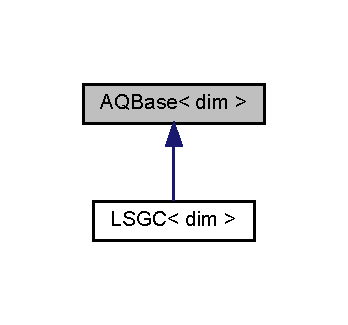
\includegraphics[width=167pt]{class_a_q_base__inherit__graph}
\end{center}
\end{figure}
\subsection*{Public Member Functions}
\begin{DoxyCompactItemize}
\item 
\hyperlink{class_a_q_base_a3a05ceb6b201b4e6e605b260d766842d}{A\+Q\+Base} (Parameter\+Handler \&prm)
\item 
virtual \hyperlink{class_a_q_base_ab394068aae3c9b3f3932c3bfa3edceab}{$\sim$\+A\+Q\+Base} ()
\begin{DoxyCompactList}\small\item\em Virtual destructor. \end{DoxyCompactList}\item 
virtual void \hyperlink{class_a_q_base_a16c7871be0da6c112f547f39d50258fd}{produce\+\_\+angular\+\_\+quad} ()
\item 
virtual void \hyperlink{class_a_q_base_ab1cbcd2132328df15fb9651597e8ab48}{initialize\+\_\+component\+\_\+index} ()
\item 
void \hyperlink{class_a_q_base_ad8bf7c63bde67a2f514aea2c589983dd}{make\+\_\+aq} ()
\item 
void \hyperlink{class_a_q_base_adbe2961a0c0db888ca6a22ead08732eb}{print\+\_\+angular\+\_\+quad} ()
\item 
unsigned int \hyperlink{class_a_q_base_a9ce78884d13c584a8f415c16976ea6f0}{get\+\_\+sn\+\_\+order} ()
\item 
unsigned int \hyperlink{class_a_q_base_a803528777761efa898b046e374008744}{get\+\_\+n\+\_\+dir} ()
\item 
unsigned int \hyperlink{class_a_q_base_af367f668495d928c27a985b081868c6c}{get\+\_\+n\+\_\+total\+\_\+ho\+\_\+vars} ()
\item 
std\+::vector$<$ double $>$ \hyperlink{class_a_q_base_ac3db7e901486ff088e4eac2f1401f3b6}{get\+\_\+angular\+\_\+weights} ()
\item 
std\+::vector$<$ Tensor$<$ 1, dim $>$ $>$ \hyperlink{class_a_q_base_ac2e0120510426f0b1dded2d5b546038b}{get\+\_\+all\+\_\+directions} ()
\item 
std\+::map$<$ std\+::pair$<$ unsigned int, unsigned int $>$, unsigned int $>$ \hyperlink{class_a_q_base_a016f7ac88052a26c82c8aa3bfba80f73}{get\+\_\+component\+\_\+index\+\_\+map} ()
\item 
std\+::unordered\+\_\+map$<$ unsigned int, std\+::pair$<$ unsigned int, unsigned int $>$ $>$ \hyperlink{class_a_q_base_a6c6f10b941afa4019a5d919eee33ebee}{get\+\_\+inv\+\_\+component\+\_\+map} ()
\item 
std\+::map$<$ std\+::pair$<$ unsigned int, unsigned int $>$, unsigned int $>$ \hyperlink{class_a_q_base_a1cb901657861f7fc580fc29e10c0b691}{get\+\_\+reflective\+\_\+direction\+\_\+index\+\_\+map} ()
\end{DoxyCompactItemize}
\subsection*{Protected Attributes}
\begin{DoxyCompactItemize}
\item 
const double \hyperlink{class_a_q_base_a002ce18f617db787616e60fba67899a9}{pi}
\begin{DoxyCompactList}\small\item\em Constant PI, 3.\+14159... \end{DoxyCompactList}\item 
double \hyperlink{class_a_q_base_a930e1dbffe2c99f42b76ea3164905ac1}{total\+\_\+angle}
\begin{DoxyCompactList}\small\item\em Total solid angle. \end{DoxyCompactList}\item 
bool \hyperlink{class_a_q_base_a8afa1e0da5bbb4846e495178e165b5b5}{have\+\_\+reflective\+\_\+bc}
\begin{DoxyCompactList}\small\item\em Boolean about if there is any reflective boundary. \end{DoxyCompactList}\item 
std\+::string \hyperlink{class_a_q_base_a14d94b7179306f35228b90fd5f42c65a}{transport\+\_\+model\+\_\+name}
\begin{DoxyCompactList}\small\item\em Transport model name in string. \end{DoxyCompactList}\item 
std\+::string \hyperlink{class_a_q_base_a6c454af11008e235340a7b8e31a02114}{discretization}
\begin{DoxyCompactList}\small\item\em Spatial discretization method in string. \end{DoxyCompactList}\item 
unsigned int \hyperlink{class_a_q_base_aaff6bd848436445d267c1a121a93e4ea}{n\+\_\+azi}
\begin{DoxyCompactList}\small\item\em Total number of azimuthal angles. \end{DoxyCompactList}\item 
unsigned int \hyperlink{class_a_q_base_a07b0839db1844f879f3d9c7d7014fb7f}{n\+\_\+group}
\begin{DoxyCompactList}\small\item\em Total number of groups. \end{DoxyCompactList}\item 
unsigned int \hyperlink{class_a_q_base_a93b0c70dd1d3ec401601ceaca88723b1}{n\+\_\+dir}
\begin{DoxyCompactList}\small\item\em Total number of directions in the quadrature. \end{DoxyCompactList}\item 
unsigned int \hyperlink{class_a_q_base_a7169f8e3b53059317bb2144519f64be9}{n\+\_\+total\+\_\+ho\+\_\+vars}
\begin{DoxyCompactList}\small\item\em Total number of components in HO equation. \end{DoxyCompactList}\item 
std\+::vector$<$ Tensor$<$ 1, dim $>$ $>$ \hyperlink{class_a_q_base_a07aaf517b03be3f8405fd4063cf59231}{omega\+\_\+i}
\begin{DoxyCompactList}\small\item\em All directions in Tensor$<$1, dim$>$ \end{DoxyCompactList}\item 
std\+::vector$<$ double $>$ \hyperlink{class_a_q_base_aa43b0232837b86e608da7507bd9a14b5}{wi}
\begin{DoxyCompactList}\small\item\em All angular weights. \end{DoxyCompactList}\item 
std\+::map$<$ std\+::pair$<$ unsigned int, unsigned int $>$, unsigned int $>$ \hyperlink{class_a_q_base_a0d9e9c6302e481718d62d76c09c83d2d}{component\+\_\+index}
\item 
std\+::unordered\+\_\+map$<$ unsigned int, std\+::pair$<$ unsigned int, unsigned int $>$ $>$ \hyperlink{class_a_q_base_a657640cc73cef6130bdf5b325dd0fd11}{inverse\+\_\+component\+\_\+index}
\item 
std\+::map$<$ std\+::pair$<$ unsigned int, unsigned int $>$, unsigned int $>$ \hyperlink{class_a_q_base_a9aa6c274dd0ef167528bbec76637cc22}{reflective\+\_\+direction\+\_\+index}
\end{DoxyCompactItemize}
\subsection*{Private Member Functions}
\begin{DoxyCompactItemize}
\item 
std\+::string \hyperlink{class_a_q_base_a4ae1370033705c82d08686fd651ad6e8}{produce\+\_\+quadrature\+\_\+name} ()
\item 
void \hyperlink{class_a_q_base_aafde5b4c9ce19b1c6c4a8d37787f13b2}{initialize\+\_\+ref\+\_\+bc\+\_\+index} ()
\end{DoxyCompactItemize}
\subsection*{Private Attributes}
\begin{DoxyCompactItemize}
\item 
std\+::string \hyperlink{class_a_q_base_a3e50d2d59d1a4a2fabed3c4852f80c49}{aq\+\_\+name}
\end{DoxyCompactItemize}


\subsection{Detailed Description}
\subsubsection*{template$<$int dim$>$\newline
class A\+Q\+Base$<$ dim $>$}

This class provides AQ data, component indices and reflective directions. 

This class is the base class of AQ data. The directions are represented by a series of \href{https://www.dealii.org/8.5.0/doxygen/deal.II/classTensor.htm
l}{\tt {\bfseries Tensor$<$1,dim$>$}}. deal.\+II has well defined operations such as dot product of tensors.

\begin{DoxyAuthor}{Author}
Weixiong Zheng 
\end{DoxyAuthor}
\begin{DoxyDate}{Date}
2017/04 
\end{DoxyDate}


Definition at line 25 of file aq\+\_\+base.\+h.



\subsection{Constructor \& Destructor Documentation}
\mbox{\Hypertarget{class_a_q_base_a3a05ceb6b201b4e6e605b260d766842d}\label{class_a_q_base_a3a05ceb6b201b4e6e605b260d766842d}} 
\index{A\+Q\+Base@{A\+Q\+Base}!A\+Q\+Base@{A\+Q\+Base}}
\index{A\+Q\+Base@{A\+Q\+Base}!A\+Q\+Base@{A\+Q\+Base}}
\subsubsection{\texorpdfstring{A\+Q\+Base()}{AQBase()}}
{\footnotesize\ttfamily template$<$int dim$>$ \\
\hyperlink{class_a_q_base}{A\+Q\+Base}$<$ dim $>$\+::\hyperlink{class_a_q_base}{A\+Q\+Base} (\begin{DoxyParamCaption}\item[{Parameter\+Handler \&}]{prm }\end{DoxyParamCaption})}

Class constructor.


\begin{DoxyParams}{Parameters}
{\em prm} & Parameter\+Handler object. \\
\hline
\end{DoxyParams}


Definition at line 8 of file aq\+\_\+base.\+cc.

Here is the call graph for this function\+:\nopagebreak
\begin{figure}[H]
\begin{center}
\leavevmode
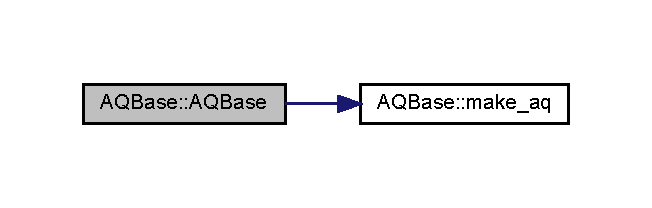
\includegraphics[width=313pt]{class_a_q_base_a3a05ceb6b201b4e6e605b260d766842d_cgraph}
\end{center}
\end{figure}
\mbox{\Hypertarget{class_a_q_base_ab394068aae3c9b3f3932c3bfa3edceab}\label{class_a_q_base_ab394068aae3c9b3f3932c3bfa3edceab}} 
\index{A\+Q\+Base@{A\+Q\+Base}!````~A\+Q\+Base@{$\sim$\+A\+Q\+Base}}
\index{````~A\+Q\+Base@{$\sim$\+A\+Q\+Base}!A\+Q\+Base@{A\+Q\+Base}}
\subsubsection{\texorpdfstring{$\sim$\+A\+Q\+Base()}{~AQBase()}}
{\footnotesize\ttfamily template$<$int dim$>$ \\
\hyperlink{class_a_q_base}{A\+Q\+Base}$<$ dim $>$\+::$\sim$\hyperlink{class_a_q_base}{A\+Q\+Base} (\begin{DoxyParamCaption}{ }\end{DoxyParamCaption})\hspace{0.3cm}{\ttfamily [virtual]}}



Virtual destructor. 



Definition at line 21 of file aq\+\_\+base.\+cc.



\subsection{Member Function Documentation}
\mbox{\Hypertarget{class_a_q_base_ac2e0120510426f0b1dded2d5b546038b}\label{class_a_q_base_ac2e0120510426f0b1dded2d5b546038b}} 
\index{A\+Q\+Base@{A\+Q\+Base}!get\+\_\+all\+\_\+directions@{get\+\_\+all\+\_\+directions}}
\index{get\+\_\+all\+\_\+directions@{get\+\_\+all\+\_\+directions}!A\+Q\+Base@{A\+Q\+Base}}
\subsubsection{\texorpdfstring{get\+\_\+all\+\_\+directions()}{get\_all\_directions()}}
{\footnotesize\ttfamily template$<$int dim$>$ \\
std\+::vector$<$ Tensor$<$ 1, dim $>$ $>$ \hyperlink{class_a_q_base}{A\+Q\+Base}$<$ dim $>$\+::get\+\_\+all\+\_\+directions (\begin{DoxyParamCaption}{ }\end{DoxyParamCaption})}

A function to return all the directions.

\begin{DoxyReturn}{Returns}
A vector of dealii\+::\+Tensor$<$1, dim$>$ representing directions. 
\end{DoxyReturn}


Definition at line 185 of file aq\+\_\+base.\+cc.

\mbox{\Hypertarget{class_a_q_base_ac3db7e901486ff088e4eac2f1401f3b6}\label{class_a_q_base_ac3db7e901486ff088e4eac2f1401f3b6}} 
\index{A\+Q\+Base@{A\+Q\+Base}!get\+\_\+angular\+\_\+weights@{get\+\_\+angular\+\_\+weights}}
\index{get\+\_\+angular\+\_\+weights@{get\+\_\+angular\+\_\+weights}!A\+Q\+Base@{A\+Q\+Base}}
\subsubsection{\texorpdfstring{get\+\_\+angular\+\_\+weights()}{get\_angular\_weights()}}
{\footnotesize\ttfamily template$<$int dim$>$ \\
std\+::vector$<$ double $>$ \hyperlink{class_a_q_base}{A\+Q\+Base}$<$ dim $>$\+::get\+\_\+angular\+\_\+weights (\begin{DoxyParamCaption}{ }\end{DoxyParamCaption})}

A function to return A\+Q\+Base$<$dim$>$\+::wi.

\begin{DoxyReturn}{Returns}
A vector of all angular weights. 
\end{DoxyReturn}


Definition at line 179 of file aq\+\_\+base.\+cc.

\mbox{\Hypertarget{class_a_q_base_a016f7ac88052a26c82c8aa3bfba80f73}\label{class_a_q_base_a016f7ac88052a26c82c8aa3bfba80f73}} 
\index{A\+Q\+Base@{A\+Q\+Base}!get\+\_\+component\+\_\+index\+\_\+map@{get\+\_\+component\+\_\+index\+\_\+map}}
\index{get\+\_\+component\+\_\+index\+\_\+map@{get\+\_\+component\+\_\+index\+\_\+map}!A\+Q\+Base@{A\+Q\+Base}}
\subsubsection{\texorpdfstring{get\+\_\+component\+\_\+index\+\_\+map()}{get\_component\_index\_map()}}
{\footnotesize\ttfamily template$<$int dim$>$ \\
std\+::map$<$ std\+::pair$<$ unsigned int, unsigned int $>$, unsigned int $>$ \hyperlink{class_a_q_base}{A\+Q\+Base}$<$ dim $>$\+::get\+\_\+component\+\_\+index\+\_\+map (\begin{DoxyParamCaption}{ }\end{DoxyParamCaption})}

A function to return HO component indices, A\+Q\+Base$<$dim$>$\+::component\+\_\+index.

\begin{DoxyReturn}{Returns}
A std\+::map for (group\+\_\+idx, dir\+\_\+idx)-\/$>$component\+\_\+idx. 
\end{DoxyReturn}


Definition at line 141 of file aq\+\_\+base.\+cc.

\mbox{\Hypertarget{class_a_q_base_a6c6f10b941afa4019a5d919eee33ebee}\label{class_a_q_base_a6c6f10b941afa4019a5d919eee33ebee}} 
\index{A\+Q\+Base@{A\+Q\+Base}!get\+\_\+inv\+\_\+component\+\_\+map@{get\+\_\+inv\+\_\+component\+\_\+map}}
\index{get\+\_\+inv\+\_\+component\+\_\+map@{get\+\_\+inv\+\_\+component\+\_\+map}!A\+Q\+Base@{A\+Q\+Base}}
\subsubsection{\texorpdfstring{get\+\_\+inv\+\_\+component\+\_\+map()}{get\_inv\_component\_map()}}
{\footnotesize\ttfamily template$<$int dim$>$ \\
std\+::unordered\+\_\+map$<$ unsigned int, std\+::pair$<$ unsigned int, unsigned int $>$ $>$ \hyperlink{class_a_q_base}{A\+Q\+Base}$<$ dim $>$\+::get\+\_\+inv\+\_\+component\+\_\+map (\begin{DoxyParamCaption}{ }\end{DoxyParamCaption})}

A function to return A\+Q\+Base$<$dim$>$\+::inverse\+\_\+component\+\_\+index.

\begin{DoxyReturn}{Returns}
A Hash table for component\+\_\+idx-\/$>$(group\+\_\+idx, dir\+\_\+idx). 
\end{DoxyReturn}


Definition at line 148 of file aq\+\_\+base.\+cc.

\mbox{\Hypertarget{class_a_q_base_a803528777761efa898b046e374008744}\label{class_a_q_base_a803528777761efa898b046e374008744}} 
\index{A\+Q\+Base@{A\+Q\+Base}!get\+\_\+n\+\_\+dir@{get\+\_\+n\+\_\+dir}}
\index{get\+\_\+n\+\_\+dir@{get\+\_\+n\+\_\+dir}!A\+Q\+Base@{A\+Q\+Base}}
\subsubsection{\texorpdfstring{get\+\_\+n\+\_\+dir()}{get\_n\_dir()}}
{\footnotesize\ttfamily template$<$int dim$>$ \\
unsigned int \hyperlink{class_a_q_base}{A\+Q\+Base}$<$ dim $>$\+::get\+\_\+n\+\_\+dir (\begin{DoxyParamCaption}{ }\end{DoxyParamCaption})}

A function to return total number of directions.

\begin{DoxyReturn}{Returns}
Total number of directions in integer. 
\end{DoxyReturn}


Definition at line 167 of file aq\+\_\+base.\+cc.

\mbox{\Hypertarget{class_a_q_base_af367f668495d928c27a985b081868c6c}\label{class_a_q_base_af367f668495d928c27a985b081868c6c}} 
\index{A\+Q\+Base@{A\+Q\+Base}!get\+\_\+n\+\_\+total\+\_\+ho\+\_\+vars@{get\+\_\+n\+\_\+total\+\_\+ho\+\_\+vars}}
\index{get\+\_\+n\+\_\+total\+\_\+ho\+\_\+vars@{get\+\_\+n\+\_\+total\+\_\+ho\+\_\+vars}!A\+Q\+Base@{A\+Q\+Base}}
\subsubsection{\texorpdfstring{get\+\_\+n\+\_\+total\+\_\+ho\+\_\+vars()}{get\_n\_total\_ho\_vars()}}
{\footnotesize\ttfamily template$<$int dim$>$ \\
unsigned int \hyperlink{class_a_q_base}{A\+Q\+Base}$<$ dim $>$\+::get\+\_\+n\+\_\+total\+\_\+ho\+\_\+vars (\begin{DoxyParamCaption}{ }\end{DoxyParamCaption})}

A function to return total number of components in HO equation.

\begin{DoxyReturn}{Returns}
Total number of components in HO equation. 
\end{DoxyReturn}


Definition at line 173 of file aq\+\_\+base.\+cc.

\mbox{\Hypertarget{class_a_q_base_a1cb901657861f7fc580fc29e10c0b691}\label{class_a_q_base_a1cb901657861f7fc580fc29e10c0b691}} 
\index{A\+Q\+Base@{A\+Q\+Base}!get\+\_\+reflective\+\_\+direction\+\_\+index\+\_\+map@{get\+\_\+reflective\+\_\+direction\+\_\+index\+\_\+map}}
\index{get\+\_\+reflective\+\_\+direction\+\_\+index\+\_\+map@{get\+\_\+reflective\+\_\+direction\+\_\+index\+\_\+map}!A\+Q\+Base@{A\+Q\+Base}}
\subsubsection{\texorpdfstring{get\+\_\+reflective\+\_\+direction\+\_\+index\+\_\+map()}{get\_reflective\_direction\_index\_map()}}
{\footnotesize\ttfamily template$<$int dim$>$ \\
std\+::map$<$ std\+::pair$<$ unsigned int, unsigned int $>$, unsigned int $>$ \hyperlink{class_a_q_base}{A\+Q\+Base}$<$ dim $>$\+::get\+\_\+reflective\+\_\+direction\+\_\+index\+\_\+map (\begin{DoxyParamCaption}{ }\end{DoxyParamCaption})}

A function to return A\+Q\+Base$<$dim$>$\+::reflective\+\_\+direction\+\_\+index.

\begin{DoxyReturn}{Returns}
std\+::map for the mapping\+: (boundary\+\_\+id, current\+\_\+dir)-\/$>$refl\+\_\+dir. 
\end{DoxyReturn}


Definition at line 155 of file aq\+\_\+base.\+cc.

\mbox{\Hypertarget{class_a_q_base_a9ce78884d13c584a8f415c16976ea6f0}\label{class_a_q_base_a9ce78884d13c584a8f415c16976ea6f0}} 
\index{A\+Q\+Base@{A\+Q\+Base}!get\+\_\+sn\+\_\+order@{get\+\_\+sn\+\_\+order}}
\index{get\+\_\+sn\+\_\+order@{get\+\_\+sn\+\_\+order}!A\+Q\+Base@{A\+Q\+Base}}
\subsubsection{\texorpdfstring{get\+\_\+sn\+\_\+order()}{get\_sn\_order()}}
{\footnotesize\ttfamily template$<$int dim$>$ \\
unsigned int \hyperlink{class_a_q_base}{A\+Q\+Base}$<$ dim $>$\+::get\+\_\+sn\+\_\+order (\begin{DoxyParamCaption}{ }\end{DoxyParamCaption})}

A function to return SN order in integer.

\begin{DoxyReturn}{Returns}
SN order. 
\end{DoxyReturn}


Definition at line 161 of file aq\+\_\+base.\+cc.

\mbox{\Hypertarget{class_a_q_base_ab1cbcd2132328df15fb9651597e8ab48}\label{class_a_q_base_ab1cbcd2132328df15fb9651597e8ab48}} 
\index{A\+Q\+Base@{A\+Q\+Base}!initialize\+\_\+component\+\_\+index@{initialize\+\_\+component\+\_\+index}}
\index{initialize\+\_\+component\+\_\+index@{initialize\+\_\+component\+\_\+index}!A\+Q\+Base@{A\+Q\+Base}}
\subsubsection{\texorpdfstring{initialize\+\_\+component\+\_\+index()}{initialize\_component\_index()}}
{\footnotesize\ttfamily template$<$int dim$>$ \\
void \hyperlink{class_a_q_base}{A\+Q\+Base}$<$ dim $>$\+::initialize\+\_\+component\+\_\+index (\begin{DoxyParamCaption}{ }\end{DoxyParamCaption})\hspace{0.3cm}{\ttfamily [virtual]}}



Definition at line 91 of file aq\+\_\+base.\+cc.

\mbox{\Hypertarget{class_a_q_base_aafde5b4c9ce19b1c6c4a8d37787f13b2}\label{class_a_q_base_aafde5b4c9ce19b1c6c4a8d37787f13b2}} 
\index{A\+Q\+Base@{A\+Q\+Base}!initialize\+\_\+ref\+\_\+bc\+\_\+index@{initialize\+\_\+ref\+\_\+bc\+\_\+index}}
\index{initialize\+\_\+ref\+\_\+bc\+\_\+index@{initialize\+\_\+ref\+\_\+bc\+\_\+index}!A\+Q\+Base@{A\+Q\+Base}}
\subsubsection{\texorpdfstring{initialize\+\_\+ref\+\_\+bc\+\_\+index()}{initialize\_ref\_bc\_index()}}
{\footnotesize\ttfamily template$<$int dim$>$ \\
void \hyperlink{class_a_q_base}{A\+Q\+Base}$<$ dim $>$\+::initialize\+\_\+ref\+\_\+bc\+\_\+index (\begin{DoxyParamCaption}{ }\end{DoxyParamCaption})\hspace{0.3cm}{\ttfamily [private]}}

This function initialize reflective direction indices on all boundaries. If A\+Q\+Base$<$dim$>$\+::have\+\_\+reflective\+\_\+bc is true, this function will generate such indices for all boundaries and result in std\+::map using std\+::pair of boundary id and current direction index as the key and reflective direction index as the value.

\begin{DoxyReturn}{Returns}
Void. 
\end{DoxyReturn}


Definition at line 34 of file aq\+\_\+base.\+cc.

\mbox{\Hypertarget{class_a_q_base_ad8bf7c63bde67a2f514aea2c589983dd}\label{class_a_q_base_ad8bf7c63bde67a2f514aea2c589983dd}} 
\index{A\+Q\+Base@{A\+Q\+Base}!make\+\_\+aq@{make\+\_\+aq}}
\index{make\+\_\+aq@{make\+\_\+aq}!A\+Q\+Base@{A\+Q\+Base}}
\subsubsection{\texorpdfstring{make\+\_\+aq()}{make\_aq()}}
{\footnotesize\ttfamily template$<$int dim$>$ \\
void \hyperlink{class_a_q_base}{A\+Q\+Base}$<$ dim $>$\+::make\+\_\+aq (\begin{DoxyParamCaption}{ }\end{DoxyParamCaption})}

This function calls other members to\+:

(1) Create aq data;

(2) Create indices of components in transport system;

(3) Create indices of reflective directions for all directions in the aq on all boundaries.

\begin{DoxyReturn}{Returns}
Void. 
\end{DoxyReturn}


Definition at line 26 of file aq\+\_\+base.\+cc.

Here is the caller graph for this function\+:\nopagebreak
\begin{figure}[H]
\begin{center}
\leavevmode
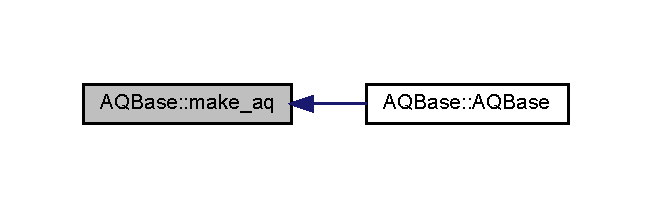
\includegraphics[width=313pt]{class_a_q_base_ad8bf7c63bde67a2f514aea2c589983dd_icgraph}
\end{center}
\end{figure}
\mbox{\Hypertarget{class_a_q_base_adbe2961a0c0db888ca6a22ead08732eb}\label{class_a_q_base_adbe2961a0c0db888ca6a22ead08732eb}} 
\index{A\+Q\+Base@{A\+Q\+Base}!print\+\_\+angular\+\_\+quad@{print\+\_\+angular\+\_\+quad}}
\index{print\+\_\+angular\+\_\+quad@{print\+\_\+angular\+\_\+quad}!A\+Q\+Base@{A\+Q\+Base}}
\subsubsection{\texorpdfstring{print\+\_\+angular\+\_\+quad()}{print\_angular\_quad()}}
{\footnotesize\ttfamily template$<$int dim$>$ \\
void \hyperlink{class_a_q_base}{A\+Q\+Base}$<$ dim $>$\+::print\+\_\+angular\+\_\+quad (\begin{DoxyParamCaption}{ }\end{DoxyParamCaption})}

This function output angular quadrature in aq.\+txt file.

\begin{DoxyReturn}{Returns}
Void. 
\end{DoxyReturn}


Definition at line 106 of file aq\+\_\+base.\+cc.

\mbox{\Hypertarget{class_a_q_base_a16c7871be0da6c112f547f39d50258fd}\label{class_a_q_base_a16c7871be0da6c112f547f39d50258fd}} 
\index{A\+Q\+Base@{A\+Q\+Base}!produce\+\_\+angular\+\_\+quad@{produce\+\_\+angular\+\_\+quad}}
\index{produce\+\_\+angular\+\_\+quad@{produce\+\_\+angular\+\_\+quad}!A\+Q\+Base@{A\+Q\+Base}}
\subsubsection{\texorpdfstring{produce\+\_\+angular\+\_\+quad()}{produce\_angular\_quad()}}
{\footnotesize\ttfamily template$<$int dim$>$ \\
void \hyperlink{class_a_q_base}{A\+Q\+Base}$<$ dim $>$\+::produce\+\_\+angular\+\_\+quad (\begin{DoxyParamCaption}{ }\end{DoxyParamCaption})\hspace{0.3cm}{\ttfamily [virtual]}}

A virtual function to produce angular quadrature.

\begin{DoxyNote}{Note}
One has to override this function in derived classes. 
\end{DoxyNote}
\begin{DoxyReturn}{Returns}
Void. 
\end{DoxyReturn}


Reimplemented in \hyperlink{class_l_s_g_c_a1d135fb9ca12a9b65b8cc397479fc4d7}{L\+S\+G\+C$<$ dim $>$}.



Definition at line 86 of file aq\+\_\+base.\+cc.

\mbox{\Hypertarget{class_a_q_base_a4ae1370033705c82d08686fd651ad6e8}\label{class_a_q_base_a4ae1370033705c82d08686fd651ad6e8}} 
\index{A\+Q\+Base@{A\+Q\+Base}!produce\+\_\+quadrature\+\_\+name@{produce\+\_\+quadrature\+\_\+name}}
\index{produce\+\_\+quadrature\+\_\+name@{produce\+\_\+quadrature\+\_\+name}!A\+Q\+Base@{A\+Q\+Base}}
\subsubsection{\texorpdfstring{produce\+\_\+quadrature\+\_\+name()}{produce\_quadrature\_name()}}
{\footnotesize\ttfamily template$<$int dim$>$ \\
std\+::string \hyperlink{class_a_q_base}{A\+Q\+Base}$<$ dim $>$\+::produce\+\_\+quadrature\+\_\+name (\begin{DoxyParamCaption}{ }\end{DoxyParamCaption})\hspace{0.3cm}{\ttfamily [private]}}

This function returns full name of the angular quadrature in string based on the abbreviated name.

\begin{DoxyReturn}{Returns}
Full AQ name in string. 
\end{DoxyReturn}


Definition at line 129 of file aq\+\_\+base.\+cc.



\subsection{Member Data Documentation}
\mbox{\Hypertarget{class_a_q_base_a3e50d2d59d1a4a2fabed3c4852f80c49}\label{class_a_q_base_a3e50d2d59d1a4a2fabed3c4852f80c49}} 
\index{A\+Q\+Base@{A\+Q\+Base}!aq\+\_\+name@{aq\+\_\+name}}
\index{aq\+\_\+name@{aq\+\_\+name}!A\+Q\+Base@{A\+Q\+Base}}
\subsubsection{\texorpdfstring{aq\+\_\+name}{aq\_name}}
{\footnotesize\ttfamily template$<$int dim$>$ \\
std\+::string \hyperlink{class_a_q_base}{A\+Q\+Base}$<$ dim $>$\+::aq\+\_\+name\hspace{0.3cm}{\ttfamily [private]}}



Definition at line 180 of file aq\+\_\+base.\+h.

\mbox{\Hypertarget{class_a_q_base_a0d9e9c6302e481718d62d76c09c83d2d}\label{class_a_q_base_a0d9e9c6302e481718d62d76c09c83d2d}} 
\index{A\+Q\+Base@{A\+Q\+Base}!component\+\_\+index@{component\+\_\+index}}
\index{component\+\_\+index@{component\+\_\+index}!A\+Q\+Base@{A\+Q\+Base}}
\subsubsection{\texorpdfstring{component\+\_\+index}{component\_index}}
{\footnotesize\ttfamily template$<$int dim$>$ \\
std\+::map$<$std\+::pair$<$unsigned int, unsigned int$>$, unsigned int$>$ \hyperlink{class_a_q_base}{A\+Q\+Base}$<$ dim $>$\+::component\+\_\+index\hspace{0.3cm}{\ttfamily [protected]}}

A std\+::map using pair of group and direction indices as key and component index as value. 

Definition at line 145 of file aq\+\_\+base.\+h.

\mbox{\Hypertarget{class_a_q_base_a6c454af11008e235340a7b8e31a02114}\label{class_a_q_base_a6c454af11008e235340a7b8e31a02114}} 
\index{A\+Q\+Base@{A\+Q\+Base}!discretization@{discretization}}
\index{discretization@{discretization}!A\+Q\+Base@{A\+Q\+Base}}
\subsubsection{\texorpdfstring{discretization}{discretization}}
{\footnotesize\ttfamily template$<$int dim$>$ \\
std\+::string \hyperlink{class_a_q_base}{A\+Q\+Base}$<$ dim $>$\+::discretization\hspace{0.3cm}{\ttfamily [protected]}}



Spatial discretization method in string. 



Definition at line 132 of file aq\+\_\+base.\+h.

\mbox{\Hypertarget{class_a_q_base_a8afa1e0da5bbb4846e495178e165b5b5}\label{class_a_q_base_a8afa1e0da5bbb4846e495178e165b5b5}} 
\index{A\+Q\+Base@{A\+Q\+Base}!have\+\_\+reflective\+\_\+bc@{have\+\_\+reflective\+\_\+bc}}
\index{have\+\_\+reflective\+\_\+bc@{have\+\_\+reflective\+\_\+bc}!A\+Q\+Base@{A\+Q\+Base}}
\subsubsection{\texorpdfstring{have\+\_\+reflective\+\_\+bc}{have\_reflective\_bc}}
{\footnotesize\ttfamily template$<$int dim$>$ \\
bool \hyperlink{class_a_q_base}{A\+Q\+Base}$<$ dim $>$\+::have\+\_\+reflective\+\_\+bc\hspace{0.3cm}{\ttfamily [protected]}}



Boolean about if there is any reflective boundary. 



Definition at line 130 of file aq\+\_\+base.\+h.

\mbox{\Hypertarget{class_a_q_base_a657640cc73cef6130bdf5b325dd0fd11}\label{class_a_q_base_a657640cc73cef6130bdf5b325dd0fd11}} 
\index{A\+Q\+Base@{A\+Q\+Base}!inverse\+\_\+component\+\_\+index@{inverse\+\_\+component\+\_\+index}}
\index{inverse\+\_\+component\+\_\+index@{inverse\+\_\+component\+\_\+index}!A\+Q\+Base@{A\+Q\+Base}}
\subsubsection{\texorpdfstring{inverse\+\_\+component\+\_\+index}{inverse\_component\_index}}
{\footnotesize\ttfamily template$<$int dim$>$ \\
std\+::unordered\+\_\+map$<$unsigned int, std\+::pair$<$unsigned int, unsigned int$>$ $>$ \hyperlink{class_a_q_base}{A\+Q\+Base}$<$ dim $>$\+::inverse\+\_\+component\+\_\+index\hspace{0.3cm}{\ttfamily [protected]}}

A Hash table using component index as key and pair of group and direction indices as value. 

Definition at line 152 of file aq\+\_\+base.\+h.

\mbox{\Hypertarget{class_a_q_base_aaff6bd848436445d267c1a121a93e4ea}\label{class_a_q_base_aaff6bd848436445d267c1a121a93e4ea}} 
\index{A\+Q\+Base@{A\+Q\+Base}!n\+\_\+azi@{n\+\_\+azi}}
\index{n\+\_\+azi@{n\+\_\+azi}!A\+Q\+Base@{A\+Q\+Base}}
\subsubsection{\texorpdfstring{n\+\_\+azi}{n\_azi}}
{\footnotesize\ttfamily template$<$int dim$>$ \\
unsigned int \hyperlink{class_a_q_base}{A\+Q\+Base}$<$ dim $>$\+::n\+\_\+azi\hspace{0.3cm}{\ttfamily [protected]}}



Total number of azimuthal angles. 



Definition at line 133 of file aq\+\_\+base.\+h.

\mbox{\Hypertarget{class_a_q_base_a93b0c70dd1d3ec401601ceaca88723b1}\label{class_a_q_base_a93b0c70dd1d3ec401601ceaca88723b1}} 
\index{A\+Q\+Base@{A\+Q\+Base}!n\+\_\+dir@{n\+\_\+dir}}
\index{n\+\_\+dir@{n\+\_\+dir}!A\+Q\+Base@{A\+Q\+Base}}
\subsubsection{\texorpdfstring{n\+\_\+dir}{n\_dir}}
{\footnotesize\ttfamily template$<$int dim$>$ \\
unsigned int \hyperlink{class_a_q_base}{A\+Q\+Base}$<$ dim $>$\+::n\+\_\+dir\hspace{0.3cm}{\ttfamily [protected]}}



Total number of directions in the quadrature. 



Definition at line 135 of file aq\+\_\+base.\+h.

\mbox{\Hypertarget{class_a_q_base_a07b0839db1844f879f3d9c7d7014fb7f}\label{class_a_q_base_a07b0839db1844f879f3d9c7d7014fb7f}} 
\index{A\+Q\+Base@{A\+Q\+Base}!n\+\_\+group@{n\+\_\+group}}
\index{n\+\_\+group@{n\+\_\+group}!A\+Q\+Base@{A\+Q\+Base}}
\subsubsection{\texorpdfstring{n\+\_\+group}{n\_group}}
{\footnotesize\ttfamily template$<$int dim$>$ \\
unsigned int \hyperlink{class_a_q_base}{A\+Q\+Base}$<$ dim $>$\+::n\+\_\+group\hspace{0.3cm}{\ttfamily [protected]}}



Total number of groups. 



Definition at line 134 of file aq\+\_\+base.\+h.

\mbox{\Hypertarget{class_a_q_base_a7169f8e3b53059317bb2144519f64be9}\label{class_a_q_base_a7169f8e3b53059317bb2144519f64be9}} 
\index{A\+Q\+Base@{A\+Q\+Base}!n\+\_\+total\+\_\+ho\+\_\+vars@{n\+\_\+total\+\_\+ho\+\_\+vars}}
\index{n\+\_\+total\+\_\+ho\+\_\+vars@{n\+\_\+total\+\_\+ho\+\_\+vars}!A\+Q\+Base@{A\+Q\+Base}}
\subsubsection{\texorpdfstring{n\+\_\+total\+\_\+ho\+\_\+vars}{n\_total\_ho\_vars}}
{\footnotesize\ttfamily template$<$int dim$>$ \\
unsigned int \hyperlink{class_a_q_base}{A\+Q\+Base}$<$ dim $>$\+::n\+\_\+total\+\_\+ho\+\_\+vars\hspace{0.3cm}{\ttfamily [protected]}}



Total number of components in HO equation. 



Definition at line 136 of file aq\+\_\+base.\+h.

\mbox{\Hypertarget{class_a_q_base_a07aaf517b03be3f8405fd4063cf59231}\label{class_a_q_base_a07aaf517b03be3f8405fd4063cf59231}} 
\index{A\+Q\+Base@{A\+Q\+Base}!omega\+\_\+i@{omega\+\_\+i}}
\index{omega\+\_\+i@{omega\+\_\+i}!A\+Q\+Base@{A\+Q\+Base}}
\subsubsection{\texorpdfstring{omega\+\_\+i}{omega\_i}}
{\footnotesize\ttfamily template$<$int dim$>$ \\
std\+::vector$<$Tensor$<$1, dim$>$ $>$ \hyperlink{class_a_q_base}{A\+Q\+Base}$<$ dim $>$\+::omega\+\_\+i\hspace{0.3cm}{\ttfamily [protected]}}



All directions in Tensor$<$1, dim$>$ 



Definition at line 137 of file aq\+\_\+base.\+h.

\mbox{\Hypertarget{class_a_q_base_a002ce18f617db787616e60fba67899a9}\label{class_a_q_base_a002ce18f617db787616e60fba67899a9}} 
\index{A\+Q\+Base@{A\+Q\+Base}!pi@{pi}}
\index{pi@{pi}!A\+Q\+Base@{A\+Q\+Base}}
\subsubsection{\texorpdfstring{pi}{pi}}
{\footnotesize\ttfamily template$<$int dim$>$ \\
const double \hyperlink{class_a_q_base}{A\+Q\+Base}$<$ dim $>$\+::pi\hspace{0.3cm}{\ttfamily [protected]}}



Constant PI, 3.\+14159... 



Definition at line 128 of file aq\+\_\+base.\+h.

\mbox{\Hypertarget{class_a_q_base_a9aa6c274dd0ef167528bbec76637cc22}\label{class_a_q_base_a9aa6c274dd0ef167528bbec76637cc22}} 
\index{A\+Q\+Base@{A\+Q\+Base}!reflective\+\_\+direction\+\_\+index@{reflective\+\_\+direction\+\_\+index}}
\index{reflective\+\_\+direction\+\_\+index@{reflective\+\_\+direction\+\_\+index}!A\+Q\+Base@{A\+Q\+Base}}
\subsubsection{\texorpdfstring{reflective\+\_\+direction\+\_\+index}{reflective\_direction\_index}}
{\footnotesize\ttfamily template$<$int dim$>$ \\
std\+::map$<$std\+::pair$<$unsigned int, unsigned int$>$, unsigned int$>$ \hyperlink{class_a_q_base}{A\+Q\+Base}$<$ dim $>$\+::reflective\+\_\+direction\+\_\+index\hspace{0.3cm}{\ttfamily [protected]}}

A std\+::map using pair of boundary id and current direction index as key and reflective direction index as value. 

Definition at line 159 of file aq\+\_\+base.\+h.

\mbox{\Hypertarget{class_a_q_base_a930e1dbffe2c99f42b76ea3164905ac1}\label{class_a_q_base_a930e1dbffe2c99f42b76ea3164905ac1}} 
\index{A\+Q\+Base@{A\+Q\+Base}!total\+\_\+angle@{total\+\_\+angle}}
\index{total\+\_\+angle@{total\+\_\+angle}!A\+Q\+Base@{A\+Q\+Base}}
\subsubsection{\texorpdfstring{total\+\_\+angle}{total\_angle}}
{\footnotesize\ttfamily template$<$int dim$>$ \\
double \hyperlink{class_a_q_base}{A\+Q\+Base}$<$ dim $>$\+::total\+\_\+angle\hspace{0.3cm}{\ttfamily [protected]}}



Total solid angle. 



Definition at line 129 of file aq\+\_\+base.\+h.

\mbox{\Hypertarget{class_a_q_base_a14d94b7179306f35228b90fd5f42c65a}\label{class_a_q_base_a14d94b7179306f35228b90fd5f42c65a}} 
\index{A\+Q\+Base@{A\+Q\+Base}!transport\+\_\+model\+\_\+name@{transport\+\_\+model\+\_\+name}}
\index{transport\+\_\+model\+\_\+name@{transport\+\_\+model\+\_\+name}!A\+Q\+Base@{A\+Q\+Base}}
\subsubsection{\texorpdfstring{transport\+\_\+model\+\_\+name}{transport\_model\_name}}
{\footnotesize\ttfamily template$<$int dim$>$ \\
std\+::string \hyperlink{class_a_q_base}{A\+Q\+Base}$<$ dim $>$\+::transport\+\_\+model\+\_\+name\hspace{0.3cm}{\ttfamily [protected]}}



Transport model name in string. 



Definition at line 131 of file aq\+\_\+base.\+h.

\mbox{\Hypertarget{class_a_q_base_aa43b0232837b86e608da7507bd9a14b5}\label{class_a_q_base_aa43b0232837b86e608da7507bd9a14b5}} 
\index{A\+Q\+Base@{A\+Q\+Base}!wi@{wi}}
\index{wi@{wi}!A\+Q\+Base@{A\+Q\+Base}}
\subsubsection{\texorpdfstring{wi}{wi}}
{\footnotesize\ttfamily template$<$int dim$>$ \\
std\+::vector$<$double$>$ \hyperlink{class_a_q_base}{A\+Q\+Base}$<$ dim $>$\+::wi\hspace{0.3cm}{\ttfamily [protected]}}



All angular weights. 



Definition at line 138 of file aq\+\_\+base.\+h.



The documentation for this class was generated from the following files\+:\begin{DoxyCompactItemize}
\item 
src/aqdata/\hyperlink{aq__base_8h}{aq\+\_\+base.\+h}\item 
src/aqdata/\hyperlink{aq__base_8cc}{aq\+\_\+base.\+cc}\end{DoxyCompactItemize}

\hypertarget{class_bart_driver}{}\section{Bart\+Driver$<$ dim $>$ Class Template Reference}
\label{class_bart_driver}\index{Bart\+Driver$<$ dim $>$@{Bart\+Driver$<$ dim $>$}}


This class provides highest-\/level operations on B\+A\+RT to solve the problems.  




{\ttfamily \#include $<$bart\+\_\+driver.\+h$>$}

\subsection*{Public Member Functions}
\begin{DoxyCompactItemize}
\item 
\hyperlink{class_bart_driver_acad3b3200543d46ab9e4c78b860f822c}{Bart\+Driver} (Parameter\+Handler \&prm)
\item 
\hyperlink{class_bart_driver_aa89fe626d99cb4013b83d5e99698a9f3}{$\sim$\+Bart\+Driver} ()
\begin{DoxyCompactList}\small\item\em Destructor. \end{DoxyCompactList}\item 
void \hyperlink{class_bart_driver_a20c70ef3733fc4406353e6fdfee6c684}{run} ()
\begin{DoxyCompactList}\small\item\em Public function used to run all the functions inside it. \end{DoxyCompactList}\end{DoxyCompactItemize}
\subsection*{Private Member Functions}
\begin{DoxyCompactItemize}
\item 
void \hyperlink{class_bart_driver_ade375a4999de1e775434e11d4e6dd935}{build\+\_\+basis} (Parameter\+Handler \&prm)
\item 
void \hyperlink{class_bart_driver_a54ac94a562fa8f5cdb13ba6c56965b9c}{setup\+\_\+system} ()
\item 
void \hyperlink{class_bart_driver_aaf3b0ad2798c9add9e37ca0f649c416d}{report\+\_\+system} ()
\begin{DoxyCompactList}\small\item\em Function to print features such as SN order, number of groups etc. on screen. \end{DoxyCompactList}\item 
void \hyperlink{class_bart_driver_a1c440c9add7a5ec9d28afb7d44fa23d9}{output\+\_\+results} () const
\item 
std\+\_\+cxx11\+::shared\+\_\+ptr$<$ \hyperlink{class_equation_base}{Equation\+Base}$<$ dim $>$ $>$ \hyperlink{class_bart_driver_a10475395d7db9274b69349420460243d}{build\+\_\+equation} (std\+::string equation\+\_\+name, const Parameter\+Handler \&prm, const std\+\_\+cxx11\+::shared\+\_\+ptr$<$ \hyperlink{class_mesh_generator}{Mesh\+Generator}$<$ dim $>$ $>$ \hyperlink{class_bart_driver_a976c3ba1c98180dced85019dfd56e225}{msh\+\_\+ptr}, const std\+\_\+cxx11\+::shared\+\_\+ptr$<$ \hyperlink{class_a_q_base}{A\+Q\+Base}$<$ dim $>$ $>$ \hyperlink{class_bart_driver_a818149e4acfe5a7108ef42938650ff11}{aqd\+\_\+ptr}, const std\+\_\+cxx11\+::shared\+\_\+ptr$<$ \hyperlink{class_material_properties}{Material\+Properties} $>$ \hyperlink{class_bart_driver_aef9abac579c212463a6790a0e39e6429}{mat\+\_\+ptr})
\item 
std\+\_\+cxx11\+::shared\+\_\+ptr$<$ \hyperlink{class_a_q_base}{A\+Q\+Base}$<$ dim $>$ $>$ \hyperlink{class_bart_driver_ac5d2985a0286bdac161f3c0fbb80197a}{build\+\_\+aq\+\_\+model} (Parameter\+Handler \&prm)
\begin{DoxyCompactList}\small\item\em Function used to build pointer to instance of A\+Q\+Base\textquotesingle{}s derived class. \end{DoxyCompactList}\item 
std\+\_\+cxx11\+::shared\+\_\+ptr$<$ \hyperlink{class_eigen_base}{Eigen\+Base}$<$ dim $>$ $>$ \hyperlink{class_bart_driver_abc542028ef1ab71693acba10bf017018}{build\+\_\+eigen\+\_\+iterations} (const Parameter\+Handler \&prm)
\begin{DoxyCompactList}\small\item\em Function used to build pointer to instance of Eigen\+Base\textquotesingle{}s derived class. \end{DoxyCompactList}\item 
std\+\_\+cxx11\+::shared\+\_\+ptr$<$ \hyperlink{class_m_g_base}{M\+G\+Base}$<$ dim $>$ $>$ \hyperlink{class_bart_driver_af0c96d5fe57cdb8df75e1fb93ce6196b}{build\+\_\+mg\+\_\+iterations} (const Parameter\+Handler \&prm)
\begin{DoxyCompactList}\small\item\em Function used to build pointer to instance of M\+G\+Base\textquotesingle{}s derived class. \end{DoxyCompactList}\item 
std\+\_\+cxx11\+::shared\+\_\+ptr$<$ \hyperlink{class_i_g_base}{I\+G\+Base}$<$ dim $>$ $>$ \hyperlink{class_bart_driver_adc7ebcc2b3d02b7058410abef7e1b8a5}{build\+\_\+ig\+\_\+iterations} (const Parameter\+Handler \&prm)
\begin{DoxyCompactList}\small\item\em Function used to build pointer to instance of In\+Group\+Base\textquotesingle{}s derived class. \end{DoxyCompactList}\end{DoxyCompactItemize}
\subsection*{Private Attributes}
\begin{DoxyCompactItemize}
\item 
F\+E\+\_\+\+Poly$<$ Tensor\+Product\+Polynomials$<$ dim $>$, dim, dim $>$ $\ast$ \hyperlink{class_bart_driver_ac2e63d4ab8a403649e19f4b1acf94c04}{fe}
\begin{DoxyCompactList}\small\item\em Finite element type. \end{DoxyCompactList}\item 
parallel\+::distributed\+::\+Triangulation$<$ dim $>$ \hyperlink{class_bart_driver_a8bdcafa21b042017d1e871ed07ae3a81}{triangulation}
\begin{DoxyCompactList}\small\item\em Triangulation in distrubted system. \end{DoxyCompactList}\item 
Do\+F\+Handler$<$ dim $>$ \hyperlink{class_bart_driver_a102ccb2fc2ea225bc75f757214152c1b}{dof\+\_\+handler}
\begin{DoxyCompactList}\small\item\em Do\+F\+Handler instance. \end{DoxyCompactList}\item 
Index\+Set \hyperlink{class_bart_driver_a06a4f83c6f9bea928ec311fcdf974ab1}{local\+\_\+dofs}
\begin{DoxyCompactList}\small\item\em Index of dofs living on current processor. \end{DoxyCompactList}\item 
Index\+Set \hyperlink{class_bart_driver_aabb9851e7b41f4a4b9395d79e4653ec7}{relevant\+\_\+dofs}
\begin{DoxyCompactList}\small\item\em Index of dofs relevant to current processor. \end{DoxyCompactList}\item 
Constraint\+Matrix \hyperlink{class_bart_driver_a2414c8e66212bb95c86f1c70db4a4099}{constraints}
\begin{DoxyCompactList}\small\item\em Constraints for hanging nodes. \end{DoxyCompactList}\item 
Conditional\+O\+Stream \hyperlink{class_bart_driver_ad7bd8e33b7a6e67aa3d31527e40d18ea}{pcout}
\begin{DoxyCompactList}\small\item\em Conditional ostream, i.\+e. ostream on one processor. \end{DoxyCompactList}\item 
std\+\_\+cxx11\+::shared\+\_\+ptr$<$ \hyperlink{class_iterations}{Iterations}$<$ dim $>$ $>$ \hyperlink{class_bart_driver_ae07e7a592dd255d69685f17d98a2ecc6}{itr\+\_\+ptr}
\begin{DoxyCompactList}\small\item\em Pointer of Iterations instance. \end{DoxyCompactList}\item 
std\+\_\+cxx11\+::shared\+\_\+ptr$<$ \hyperlink{class_mesh_generator}{Mesh\+Generator}$<$ dim $>$ $>$ \hyperlink{class_bart_driver_a976c3ba1c98180dced85019dfd56e225}{msh\+\_\+ptr}
\begin{DoxyCompactList}\small\item\em Pointer of Mesh\+Generator instance. \end{DoxyCompactList}\item 
std\+\_\+cxx11\+::shared\+\_\+ptr$<$ \hyperlink{class_material_properties}{Material\+Properties} $>$ \hyperlink{class_bart_driver_aef9abac579c212463a6790a0e39e6429}{mat\+\_\+ptr}
\begin{DoxyCompactList}\small\item\em Pointer of Material\+Properties instance. \end{DoxyCompactList}\item 
std\+\_\+cxx11\+::shared\+\_\+ptr$<$ \hyperlink{class_a_q_base}{A\+Q\+Base}$<$ dim $>$ $>$ \hyperlink{class_bart_driver_a818149e4acfe5a7108ef42938650ff11}{aqd\+\_\+ptr}
\begin{DoxyCompactList}\small\item\em Pointer of A\+Q\+Base instance. \end{DoxyCompactList}\item 
std\+\_\+cxx11\+::shared\+\_\+ptr$<$ \hyperlink{class_eigen_base}{Eigen\+Base}$<$ dim $>$ $>$ \hyperlink{class_bart_driver_a90adc0f013f07a10c5d423e3506bd589}{eig\+\_\+ptr}
\begin{DoxyCompactList}\small\item\em Pointer of Eigen\+Base instance. \end{DoxyCompactList}\item 
std\+\_\+cxx11\+::shared\+\_\+ptr$<$ \hyperlink{class_m_g_base}{M\+G\+Base}$<$ dim $>$ $>$ \hyperlink{class_bart_driver_a1ae1a91d9a049ba4354c71f6ad689d74}{mg\+\_\+ptr}
\begin{DoxyCompactList}\small\item\em Pointer of M\+G\+Base instance. \end{DoxyCompactList}\item 
std\+\_\+cxx11\+::shared\+\_\+ptr$<$ \hyperlink{class_i_g_base}{I\+G\+Base}$<$ dim $>$ $>$ \hyperlink{class_bart_driver_a83323d9561c906f6094a51a5c936cea4}{ig\+\_\+ptr}
\begin{DoxyCompactList}\small\item\em Pointer of In\+Group\+Base instance. \end{DoxyCompactList}\item 
std\+::vector$<$ std\+\_\+cxx11\+::shared\+\_\+ptr$<$ \hyperlink{class_equation_base}{Equation\+Base}$<$ dim $>$ $>$ $>$ \hyperlink{class_bart_driver_a0a6f52aed8e9c22da12a99653d1acba8}{equ\+\_\+ptrs}
\begin{DoxyCompactList}\small\item\em A vector of pointers of Equation\+Base instances. \end{DoxyCompactList}\item 
std\+::string \hyperlink{class_bart_driver_a736f40f99459dc715fdb174e06626f55}{transport\+\_\+model}
\begin{DoxyCompactList}\small\item\em Name of transport model. \end{DoxyCompactList}\item 
std\+::string \hyperlink{class_bart_driver_a7dcefb31d64ad2e76d4c04a44cb26f7c}{ho\+\_\+linear\+\_\+solver\+\_\+name}
\begin{DoxyCompactList}\small\item\em Algebraic solver name. \end{DoxyCompactList}\item 
std\+::string \hyperlink{class_bart_driver_a0662a7c4208dc352aec9adf789edb463}{ho\+\_\+preconditioner\+\_\+name}
\begin{DoxyCompactList}\small\item\em Algebraic preconditioner name. \end{DoxyCompactList}\item 
std\+::string \hyperlink{class_bart_driver_a75cc884c6895beca3d3861ca226b4a3f}{discretization}
\begin{DoxyCompactList}\small\item\em Spatial discretization method. \end{DoxyCompactList}\item 
std\+::string \hyperlink{class_bart_driver_a34229e58237aaac1551db7a3ec140e1c}{namebase}
\item 
double \hyperlink{class_bart_driver_a459fab858171aa05e4618d6d9d327e87}{keff}
\begin{DoxyCompactList}\small\item\em keff result in eigenvalue problems \end{DoxyCompactList}\item 
bool \hyperlink{class_bart_driver_a6ee26434a788284182df94da5d71ca12}{is\+\_\+eigen\+\_\+problem}
\begin{DoxyCompactList}\small\item\em Boolean to determine if a problem is about eigenvalue. \end{DoxyCompactList}\item 
bool \hyperlink{class_bart_driver_acb7aa4c65a18deef5e1be7a3477d1b12}{do\+\_\+nda}
\begin{DoxyCompactList}\small\item\em Boolean to determine if N\+DA is to be used for accelerations. \end{DoxyCompactList}\item 
bool \hyperlink{class_bart_driver_ad42739169c4b4b97014c53a616f2d1ee}{have\+\_\+reflective\+\_\+bc}
\begin{DoxyCompactList}\small\item\em Boolean to determine if there is any BC are reflective. \end{DoxyCompactList}\item 
unsigned int \hyperlink{class_bart_driver_aa1694538581e7941bbda0960bd3c7e39}{n\+\_\+dir}
\begin{DoxyCompactList}\small\item\em Total number of directions in SN calculations. \end{DoxyCompactList}\item 
unsigned int \hyperlink{class_bart_driver_a3726013dac04d13b87e35cb0c3b8b557}{n\+\_\+azi}
\begin{DoxyCompactList}\small\item\em SN order. \end{DoxyCompactList}\item 
unsigned int \hyperlink{class_bart_driver_ab290f0bd63869bf124163f68e1be1a6a}{n\+\_\+total\+\_\+ho\+\_\+vars}
\begin{DoxyCompactList}\small\item\em Total number of components. \end{DoxyCompactList}\item 
unsigned int \hyperlink{class_bart_driver_aeb5a04392c80b32379b02e18acbc1126}{n\+\_\+group}
\begin{DoxyCompactList}\small\item\em Total number of energy groups. \end{DoxyCompactList}\item 
unsigned int \hyperlink{class_bart_driver_ae6c9141662b95c89b674ccdc04e9233f}{n\+\_\+material}
\begin{DoxyCompactList}\small\item\em Total number of material types. \end{DoxyCompactList}\item 
unsigned int \hyperlink{class_bart_driver_ae6d782d30c28d741bb0df46251087809}{p\+\_\+order}
\begin{DoxyCompactList}\small\item\em Polynomial order. \end{DoxyCompactList}\item 
unsigned int \hyperlink{class_bart_driver_a1ddb881c78ef92c59f2c686b320c970e}{global\+\_\+refinements}
\begin{DoxyCompactList}\small\item\em Total number of global refinements. \end{DoxyCompactList}\item 
std\+::vector$<$ Vector$<$ double $>$ $>$ \hyperlink{class_bart_driver_a560ae94f3801fb64a35fdbcd0d8a772d}{sflxes\+\_\+proc}
\end{DoxyCompactItemize}


\subsection{Detailed Description}
\subsubsection*{template$<$int dim$>$\newline
class Bart\+Driver$<$ dim $>$}

This class provides highest-\/level operations on B\+A\+RT to solve the problems. 

This class operate B\+A\+RT. The functionalities include\+:

(1) Build necessary components for B\+A\+RT, such as AQ data, mesh, equations etc. For This functionality, please see documentation for Bart\+Driver$<$dim$>$\+::build\+\_\+basis.

(2) Setting up system.

(3) Reporting system on screen.

(4) Operation calculations at highest level\+: instantiating Iterations and perform iterations.

(5) Output results for visualization.

Note that Bart\+Driver does not touch details about how one specifically solve a transport problem. It rather calls Iterations to handle the solving.

\begin{DoxyAuthor}{Author}
Weixiong Zheng 
\end{DoxyAuthor}
\begin{DoxyDate}{Date}
2017/08 
\end{DoxyDate}


Definition at line 50 of file bart\+\_\+driver.\+h.



\subsection{Constructor \& Destructor Documentation}
\mbox{\Hypertarget{class_bart_driver_acad3b3200543d46ab9e4c78b860f822c}\label{class_bart_driver_acad3b3200543d46ab9e4c78b860f822c}} 
\index{Bart\+Driver@{Bart\+Driver}!Bart\+Driver@{Bart\+Driver}}
\index{Bart\+Driver@{Bart\+Driver}!Bart\+Driver@{Bart\+Driver}}
\subsubsection{\texorpdfstring{Bart\+Driver()}{BartDriver()}}
{\footnotesize\ttfamily template$<$int dim$>$ \\
\hyperlink{class_bart_driver}{Bart\+Driver}$<$ dim $>$\+::\hyperlink{class_bart_driver}{Bart\+Driver} (\begin{DoxyParamCaption}\item[{Parameter\+Handler \&}]{prm }\end{DoxyParamCaption})}

Class constructor.


\begin{DoxyParams}{Parameters}
{\em prm} & Parameter\+Handler object containing all user defined parameters. \\
\hline
\end{DoxyParams}


Definition at line 18 of file bart\+\_\+driver.\+cc.

Here is the call graph for this function\+:\nopagebreak
\begin{figure}[H]
\begin{center}
\leavevmode
\includegraphics[width=345pt]{class_bart_driver_acad3b3200543d46ab9e4c78b860f822c_cgraph}
\end{center}
\end{figure}
\mbox{\Hypertarget{class_bart_driver_aa89fe626d99cb4013b83d5e99698a9f3}\label{class_bart_driver_aa89fe626d99cb4013b83d5e99698a9f3}} 
\index{Bart\+Driver@{Bart\+Driver}!````~Bart\+Driver@{$\sim$\+Bart\+Driver}}
\index{````~Bart\+Driver@{$\sim$\+Bart\+Driver}!Bart\+Driver@{Bart\+Driver}}
\subsubsection{\texorpdfstring{$\sim$\+Bart\+Driver()}{~BartDriver()}}
{\footnotesize\ttfamily template$<$int dim$>$ \\
\hyperlink{class_bart_driver}{Bart\+Driver}$<$ dim $>$\+::$\sim$\hyperlink{class_bart_driver}{Bart\+Driver} (\begin{DoxyParamCaption}{ }\end{DoxyParamCaption})}



Destructor. 



Definition at line 45 of file bart\+\_\+driver.\+cc.



\subsection{Member Function Documentation}
\mbox{\Hypertarget{class_bart_driver_ac5d2985a0286bdac161f3c0fbb80197a}\label{class_bart_driver_ac5d2985a0286bdac161f3c0fbb80197a}} 
\index{Bart\+Driver@{Bart\+Driver}!build\+\_\+aq\+\_\+model@{build\+\_\+aq\+\_\+model}}
\index{build\+\_\+aq\+\_\+model@{build\+\_\+aq\+\_\+model}!Bart\+Driver@{Bart\+Driver}}
\subsubsection{\texorpdfstring{build\+\_\+aq\+\_\+model()}{build\_aq\_model()}}
{\footnotesize\ttfamily template$<$int dim$>$ \\
std\+\_\+cxx11\+::shared\+\_\+ptr$<$ \hyperlink{class_a_q_base}{A\+Q\+Base}$<$ dim $>$ $>$ \hyperlink{class_bart_driver}{Bart\+Driver}$<$ dim $>$\+::build\+\_\+aq\+\_\+model (\begin{DoxyParamCaption}\item[{Parameter\+Handler \&}]{prm }\end{DoxyParamCaption})\hspace{0.3cm}{\ttfamily [private]}}



Function used to build pointer to instance of A\+Q\+Base\textquotesingle{}s derived class. 

The main functionality is to perform downcasting from base class to derived class based on derived class type defined in Parameter\+Handler object. For robustness reason, shared\+\_\+ptr instead of raw pointer is used in the casting process.


\begin{DoxyParams}{Parameters}
{\em prm} & A Parameter\+Handler object containing all parameters processed from user input. \\
\hline
\end{DoxyParams}
\begin{DoxyReturn}{Returns}
shared\+\_\+ptr pointing to A\+Q\+Base instance. 
\end{DoxyReturn}


Definition at line 146 of file bart\+\_\+driver.\+cc.

\mbox{\Hypertarget{class_bart_driver_ade375a4999de1e775434e11d4e6dd935}\label{class_bart_driver_ade375a4999de1e775434e11d4e6dd935}} 
\index{Bart\+Driver@{Bart\+Driver}!build\+\_\+basis@{build\+\_\+basis}}
\index{build\+\_\+basis@{build\+\_\+basis}!Bart\+Driver@{Bart\+Driver}}
\subsubsection{\texorpdfstring{build\+\_\+basis()}{build\_basis()}}
{\footnotesize\ttfamily template$<$int dim$>$ \\
void \hyperlink{class_bart_driver}{Bart\+Driver}$<$ dim $>$\+::build\+\_\+basis (\begin{DoxyParamCaption}\item[{Parameter\+Handler \&}]{prm }\end{DoxyParamCaption})\hspace{0.3cm}{\ttfamily [private]}}

A function invoked in Bart\+Driver constructor to build basis of B\+A\+RT. The main functionalities includes\+: (1) Building pointer to Iteration class. (2) Downcasting A\+Q\+Base and make angular quadrature. (3) Building pointer to Mesh\+Generator class for generating mesh. (4) Building pointer to Material\+Properties class for generating material properties (5) Downcasting finite element type (6) Downcasting Equation\+Base (7) Downcasting In\+Group\+Base, M\+G\+Base, Eigen\+Base


\begin{DoxyParams}{Parameters}
{\em prm} & Parameter\+Handler object containing all parameters. \\
\hline
\end{DoxyParams}
\begin{DoxyReturn}{Returns}
Void. 
\end{DoxyReturn}


Definition at line 51 of file bart\+\_\+driver.\+cc.

Here is the caller graph for this function\+:\nopagebreak
\begin{figure}[H]
\begin{center}
\leavevmode
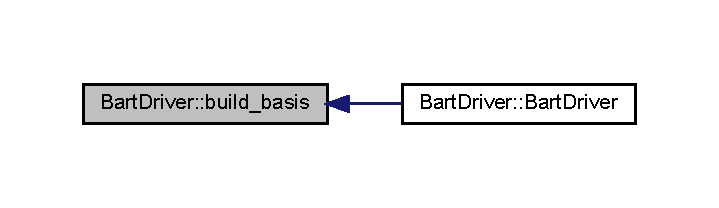
\includegraphics[width=345pt]{class_bart_driver_ade375a4999de1e775434e11d4e6dd935_icgraph}
\end{center}
\end{figure}
\mbox{\Hypertarget{class_bart_driver_abc542028ef1ab71693acba10bf017018}\label{class_bart_driver_abc542028ef1ab71693acba10bf017018}} 
\index{Bart\+Driver@{Bart\+Driver}!build\+\_\+eigen\+\_\+iterations@{build\+\_\+eigen\+\_\+iterations}}
\index{build\+\_\+eigen\+\_\+iterations@{build\+\_\+eigen\+\_\+iterations}!Bart\+Driver@{Bart\+Driver}}
\subsubsection{\texorpdfstring{build\+\_\+eigen\+\_\+iterations()}{build\_eigen\_iterations()}}
{\footnotesize\ttfamily template$<$int dim$>$ \\
std\+\_\+cxx11\+::shared\+\_\+ptr$<$ \hyperlink{class_eigen_base}{Eigen\+Base}$<$ dim $>$ $>$ \hyperlink{class_bart_driver}{Bart\+Driver}$<$ dim $>$\+::build\+\_\+eigen\+\_\+iterations (\begin{DoxyParamCaption}\item[{const Parameter\+Handler \&}]{prm }\end{DoxyParamCaption})\hspace{0.3cm}{\ttfamily [private]}}



Function used to build pointer to instance of Eigen\+Base\textquotesingle{}s derived class. 

The main functionality is to perform downcasting from base class to derived class based on derived class type defined in Parameter\+Handler object. For robustness reason, shared\+\_\+ptr instead of raw pointer is used in the casting process.


\begin{DoxyParams}{Parameters}
{\em prm} & A Parameter\+Handler object containing all parameters processed from user input. \\
\hline
\end{DoxyParams}
\begin{DoxyReturn}{Returns}
shared\+\_\+ptr pointing to Eigen\+Base instance. 
\end{DoxyReturn}


Definition at line 163 of file bart\+\_\+driver.\+cc.

\mbox{\Hypertarget{class_bart_driver_a10475395d7db9274b69349420460243d}\label{class_bart_driver_a10475395d7db9274b69349420460243d}} 
\index{Bart\+Driver@{Bart\+Driver}!build\+\_\+equation@{build\+\_\+equation}}
\index{build\+\_\+equation@{build\+\_\+equation}!Bart\+Driver@{Bart\+Driver}}
\subsubsection{\texorpdfstring{build\+\_\+equation()}{build\_equation()}}
{\footnotesize\ttfamily template$<$int dim$>$ \\
std\+\_\+cxx11\+::shared\+\_\+ptr$<$ \hyperlink{class_equation_base}{Equation\+Base}$<$ dim $>$ $>$ \hyperlink{class_bart_driver}{Bart\+Driver}$<$ dim $>$\+::build\+\_\+equation (\begin{DoxyParamCaption}\item[{std\+::string}]{equation\+\_\+name,  }\item[{const Parameter\+Handler \&}]{prm,  }\item[{const std\+\_\+cxx11\+::shared\+\_\+ptr$<$ \hyperlink{class_mesh_generator}{Mesh\+Generator}$<$ dim $>$ $>$}]{msh\+\_\+ptr,  }\item[{const std\+\_\+cxx11\+::shared\+\_\+ptr$<$ \hyperlink{class_a_q_base}{A\+Q\+Base}$<$ dim $>$ $>$}]{aqd\+\_\+ptr,  }\item[{const std\+\_\+cxx11\+::shared\+\_\+ptr$<$ \hyperlink{class_material_properties}{Material\+Properties} $>$}]{mat\+\_\+ptr }\end{DoxyParamCaption})\hspace{0.3cm}{\ttfamily [private]}}

Function builds pointer of Equation\+Base object, i.\+e. instance of space-\/angle solver. The main functionality is to perform downcasting from base class to derived class based on derived class type defined in Parameter\+Handler object. For robustness reason, shared\+\_\+ptr instead of raw pointer is used in the casting process.


\begin{DoxyParams}{Parameters}
{\em equation\+\_\+name} & A string defining the name of the desired equation. \\
\hline
{\em prm} & A Parameter\+Handler object containing all parameters processed from user input. \\
\hline
\end{DoxyParams}
\begin{DoxyReturn}{Returns}
shared\+\_\+ptr pointing to Equation\+Base instance. 
\end{DoxyReturn}


Definition at line 130 of file bart\+\_\+driver.\+cc.

\mbox{\Hypertarget{class_bart_driver_adc7ebcc2b3d02b7058410abef7e1b8a5}\label{class_bart_driver_adc7ebcc2b3d02b7058410abef7e1b8a5}} 
\index{Bart\+Driver@{Bart\+Driver}!build\+\_\+ig\+\_\+iterations@{build\+\_\+ig\+\_\+iterations}}
\index{build\+\_\+ig\+\_\+iterations@{build\+\_\+ig\+\_\+iterations}!Bart\+Driver@{Bart\+Driver}}
\subsubsection{\texorpdfstring{build\+\_\+ig\+\_\+iterations()}{build\_ig\_iterations()}}
{\footnotesize\ttfamily template$<$int dim$>$ \\
std\+\_\+cxx11\+::shared\+\_\+ptr$<$ \hyperlink{class_i_g_base}{I\+G\+Base}$<$ dim $>$ $>$ \hyperlink{class_bart_driver}{Bart\+Driver}$<$ dim $>$\+::build\+\_\+ig\+\_\+iterations (\begin{DoxyParamCaption}\item[{const Parameter\+Handler \&}]{prm }\end{DoxyParamCaption})\hspace{0.3cm}{\ttfamily [private]}}



Function used to build pointer to instance of In\+Group\+Base\textquotesingle{}s derived class. 



Definition at line 184 of file bart\+\_\+driver.\+cc.

\mbox{\Hypertarget{class_bart_driver_af0c96d5fe57cdb8df75e1fb93ce6196b}\label{class_bart_driver_af0c96d5fe57cdb8df75e1fb93ce6196b}} 
\index{Bart\+Driver@{Bart\+Driver}!build\+\_\+mg\+\_\+iterations@{build\+\_\+mg\+\_\+iterations}}
\index{build\+\_\+mg\+\_\+iterations@{build\+\_\+mg\+\_\+iterations}!Bart\+Driver@{Bart\+Driver}}
\subsubsection{\texorpdfstring{build\+\_\+mg\+\_\+iterations()}{build\_mg\_iterations()}}
{\footnotesize\ttfamily template$<$int dim$>$ \\
std\+\_\+cxx11\+::shared\+\_\+ptr$<$ \hyperlink{class_m_g_base}{M\+G\+Base}$<$ dim $>$ $>$ \hyperlink{class_bart_driver}{Bart\+Driver}$<$ dim $>$\+::build\+\_\+mg\+\_\+iterations (\begin{DoxyParamCaption}\item[{const Parameter\+Handler \&}]{prm }\end{DoxyParamCaption})\hspace{0.3cm}{\ttfamily [private]}}



Function used to build pointer to instance of M\+G\+Base\textquotesingle{}s derived class. 



Definition at line 174 of file bart\+\_\+driver.\+cc.

\mbox{\Hypertarget{class_bart_driver_a1c440c9add7a5ec9d28afb7d44fa23d9}\label{class_bart_driver_a1c440c9add7a5ec9d28afb7d44fa23d9}} 
\index{Bart\+Driver@{Bart\+Driver}!output\+\_\+results@{output\+\_\+results}}
\index{output\+\_\+results@{output\+\_\+results}!Bart\+Driver@{Bart\+Driver}}
\subsubsection{\texorpdfstring{output\+\_\+results()}{output\_results()}}
{\footnotesize\ttfamily template$<$int dim$>$ \\
void \hyperlink{class_bart_driver}{Bart\+Driver}$<$ dim $>$\+::output\+\_\+results (\begin{DoxyParamCaption}{ }\end{DoxyParamCaption}) const\hspace{0.3cm}{\ttfamily [private]}}

This function outputs results. The main functionality is to provide output files that can be read by Paraview or Visit.

Procedure of outputing results includes\+: (1) Output results on current processor to .vtu format files (2) Write out a .pvtu files on one processor which has access information for all .vtu files. 

Definition at line 244 of file bart\+\_\+driver.\+cc.

\mbox{\Hypertarget{class_bart_driver_aaf3b0ad2798c9add9e37ca0f649c416d}\label{class_bart_driver_aaf3b0ad2798c9add9e37ca0f649c416d}} 
\index{Bart\+Driver@{Bart\+Driver}!report\+\_\+system@{report\+\_\+system}}
\index{report\+\_\+system@{report\+\_\+system}!Bart\+Driver@{Bart\+Driver}}
\subsubsection{\texorpdfstring{report\+\_\+system()}{report\_system()}}
{\footnotesize\ttfamily template$<$int dim$>$ \\
void \hyperlink{class_bart_driver}{Bart\+Driver}$<$ dim $>$\+::report\+\_\+system (\begin{DoxyParamCaption}{ }\end{DoxyParamCaption})\hspace{0.3cm}{\ttfamily [private]}}



Function to print features such as SN order, number of groups etc. on screen. 



Definition at line 104 of file bart\+\_\+driver.\+cc.

\mbox{\Hypertarget{class_bart_driver_a20c70ef3733fc4406353e6fdfee6c684}\label{class_bart_driver_a20c70ef3733fc4406353e6fdfee6c684}} 
\index{Bart\+Driver@{Bart\+Driver}!run@{run}}
\index{run@{run}!Bart\+Driver@{Bart\+Driver}}
\subsubsection{\texorpdfstring{run()}{run()}}
{\footnotesize\ttfamily template$<$int dim$>$ \\
void \hyperlink{class_bart_driver}{Bart\+Driver}$<$ dim $>$\+::run (\begin{DoxyParamCaption}{ }\end{DoxyParamCaption})}



Public function used to run all the functions inside it. 

This is the only function callable outside of the class. 

Definition at line 289 of file bart\+\_\+driver.\+cc.

Here is the caller graph for this function\+:\nopagebreak
\begin{figure}[H]
\begin{center}
\leavevmode
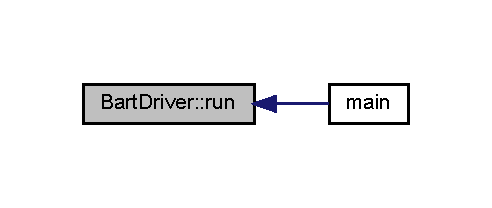
\includegraphics[width=236pt]{class_bart_driver_a20c70ef3733fc4406353e6fdfee6c684_icgraph}
\end{center}
\end{figure}
\mbox{\Hypertarget{class_bart_driver_a54ac94a562fa8f5cdb13ba6c56965b9c}\label{class_bart_driver_a54ac94a562fa8f5cdb13ba6c56965b9c}} 
\index{Bart\+Driver@{Bart\+Driver}!setup\+\_\+system@{setup\+\_\+system}}
\index{setup\+\_\+system@{setup\+\_\+system}!Bart\+Driver@{Bart\+Driver}}
\subsubsection{\texorpdfstring{setup\+\_\+system()}{setup\_system()}}
{\footnotesize\ttfamily template$<$int dim$>$ \\
void \hyperlink{class_bart_driver}{Bart\+Driver}$<$ dim $>$\+::setup\+\_\+system (\begin{DoxyParamCaption}{ }\end{DoxyParamCaption})\hspace{0.3cm}{\ttfamily [private]}}

This function initializes system settings. Main functionalities include\+: (1) Initializing dof\+\_\+handler, local\+\_\+dofs and relevant\+\_\+dofs. (2) Initializing, producing and distributing sparsity pattern (3) Initializing cell iterators on current iterators, assembly related objects and system matrices and vectors (P\+E\+T\+Sc related objects) 

Definition at line 196 of file bart\+\_\+driver.\+cc.



\subsection{Member Data Documentation}
\mbox{\Hypertarget{class_bart_driver_a818149e4acfe5a7108ef42938650ff11}\label{class_bart_driver_a818149e4acfe5a7108ef42938650ff11}} 
\index{Bart\+Driver@{Bart\+Driver}!aqd\+\_\+ptr@{aqd\+\_\+ptr}}
\index{aqd\+\_\+ptr@{aqd\+\_\+ptr}!Bart\+Driver@{Bart\+Driver}}
\subsubsection{\texorpdfstring{aqd\+\_\+ptr}{aqd\_ptr}}
{\footnotesize\ttfamily template$<$int dim$>$ \\
std\+\_\+cxx11\+::shared\+\_\+ptr$<$\hyperlink{class_a_q_base}{A\+Q\+Base}$<$dim$>$ $>$ \hyperlink{class_bart_driver}{Bart\+Driver}$<$ dim $>$\+::aqd\+\_\+ptr\hspace{0.3cm}{\ttfamily [private]}}



Pointer of A\+Q\+Base instance. 



Definition at line 199 of file bart\+\_\+driver.\+h.

\mbox{\Hypertarget{class_bart_driver_a2414c8e66212bb95c86f1c70db4a4099}\label{class_bart_driver_a2414c8e66212bb95c86f1c70db4a4099}} 
\index{Bart\+Driver@{Bart\+Driver}!constraints@{constraints}}
\index{constraints@{constraints}!Bart\+Driver@{Bart\+Driver}}
\subsubsection{\texorpdfstring{constraints}{constraints}}
{\footnotesize\ttfamily template$<$int dim$>$ \\
Constraint\+Matrix \hyperlink{class_bart_driver}{Bart\+Driver}$<$ dim $>$\+::constraints\hspace{0.3cm}{\ttfamily [private]}}



Constraints for hanging nodes. 

This will be useful if adaptive local refinement is of interest. For now, this variable is of no practical use. 

Definition at line 193 of file bart\+\_\+driver.\+h.

\mbox{\Hypertarget{class_bart_driver_a75cc884c6895beca3d3861ca226b4a3f}\label{class_bart_driver_a75cc884c6895beca3d3861ca226b4a3f}} 
\index{Bart\+Driver@{Bart\+Driver}!discretization@{discretization}}
\index{discretization@{discretization}!Bart\+Driver@{Bart\+Driver}}
\subsubsection{\texorpdfstring{discretization}{discretization}}
{\footnotesize\ttfamily template$<$int dim$>$ \\
std\+::string \hyperlink{class_bart_driver}{Bart\+Driver}$<$ dim $>$\+::discretization\hspace{0.3cm}{\ttfamily [private]}}



Spatial discretization method. 



Definition at line 215 of file bart\+\_\+driver.\+h.

\mbox{\Hypertarget{class_bart_driver_acb7aa4c65a18deef5e1be7a3477d1b12}\label{class_bart_driver_acb7aa4c65a18deef5e1be7a3477d1b12}} 
\index{Bart\+Driver@{Bart\+Driver}!do\+\_\+nda@{do\+\_\+nda}}
\index{do\+\_\+nda@{do\+\_\+nda}!Bart\+Driver@{Bart\+Driver}}
\subsubsection{\texorpdfstring{do\+\_\+nda}{do\_nda}}
{\footnotesize\ttfamily template$<$int dim$>$ \\
bool \hyperlink{class_bart_driver}{Bart\+Driver}$<$ dim $>$\+::do\+\_\+nda\hspace{0.3cm}{\ttfamily [private]}}



Boolean to determine if N\+DA is to be used for accelerations. 



Definition at line 221 of file bart\+\_\+driver.\+h.

\mbox{\Hypertarget{class_bart_driver_a102ccb2fc2ea225bc75f757214152c1b}\label{class_bart_driver_a102ccb2fc2ea225bc75f757214152c1b}} 
\index{Bart\+Driver@{Bart\+Driver}!dof\+\_\+handler@{dof\+\_\+handler}}
\index{dof\+\_\+handler@{dof\+\_\+handler}!Bart\+Driver@{Bart\+Driver}}
\subsubsection{\texorpdfstring{dof\+\_\+handler}{dof\_handler}}
{\footnotesize\ttfamily template$<$int dim$>$ \\
Do\+F\+Handler$<$dim$>$ \hyperlink{class_bart_driver}{Bart\+Driver}$<$ dim $>$\+::dof\+\_\+handler\hspace{0.3cm}{\ttfamily [private]}}



Do\+F\+Handler instance. 

Could be interpreted as a container containing smart pointers to accessors of cells (cell iterators) and relevant cell properties such as material\+\_\+id, if cell is at boundary and dof mapping between local cell and global system etc. 

Definition at line 175 of file bart\+\_\+driver.\+h.

\mbox{\Hypertarget{class_bart_driver_a90adc0f013f07a10c5d423e3506bd589}\label{class_bart_driver_a90adc0f013f07a10c5d423e3506bd589}} 
\index{Bart\+Driver@{Bart\+Driver}!eig\+\_\+ptr@{eig\+\_\+ptr}}
\index{eig\+\_\+ptr@{eig\+\_\+ptr}!Bart\+Driver@{Bart\+Driver}}
\subsubsection{\texorpdfstring{eig\+\_\+ptr}{eig\_ptr}}
{\footnotesize\ttfamily template$<$int dim$>$ \\
std\+\_\+cxx11\+::shared\+\_\+ptr$<$\hyperlink{class_eigen_base}{Eigen\+Base}$<$dim$>$ $>$ \hyperlink{class_bart_driver}{Bart\+Driver}$<$ dim $>$\+::eig\+\_\+ptr\hspace{0.3cm}{\ttfamily [private]}}



Pointer of Eigen\+Base instance. 



Definition at line 200 of file bart\+\_\+driver.\+h.

\mbox{\Hypertarget{class_bart_driver_a0a6f52aed8e9c22da12a99653d1acba8}\label{class_bart_driver_a0a6f52aed8e9c22da12a99653d1acba8}} 
\index{Bart\+Driver@{Bart\+Driver}!equ\+\_\+ptrs@{equ\+\_\+ptrs}}
\index{equ\+\_\+ptrs@{equ\+\_\+ptrs}!Bart\+Driver@{Bart\+Driver}}
\subsubsection{\texorpdfstring{equ\+\_\+ptrs}{equ\_ptrs}}
{\footnotesize\ttfamily template$<$int dim$>$ \\
std\+::vector$<$std\+\_\+cxx11\+::shared\+\_\+ptr$<$\hyperlink{class_equation_base}{Equation\+Base}$<$dim$>$ $>$ $>$ \hyperlink{class_bart_driver}{Bart\+Driver}$<$ dim $>$\+::equ\+\_\+ptrs\hspace{0.3cm}{\ttfamily [private]}}



A vector of pointers of Equation\+Base instances. 

The rule is if N\+DA is not used, this vector only has one component for transport model. Otherwise, std\+::vector\+::front() contains the pointer of HO equation and std\+::vector\+::back() contains the pointer of N\+DA equation. 

Definition at line 210 of file bart\+\_\+driver.\+h.

\mbox{\Hypertarget{class_bart_driver_ac2e63d4ab8a403649e19f4b1acf94c04}\label{class_bart_driver_ac2e63d4ab8a403649e19f4b1acf94c04}} 
\index{Bart\+Driver@{Bart\+Driver}!fe@{fe}}
\index{fe@{fe}!Bart\+Driver@{Bart\+Driver}}
\subsubsection{\texorpdfstring{fe}{fe}}
{\footnotesize\ttfamily template$<$int dim$>$ \\
F\+E\+\_\+\+Poly$<$Tensor\+Product\+Polynomials$<$dim$>$,dim,dim$>$$\ast$ \hyperlink{class_bart_driver}{Bart\+Driver}$<$ dim $>$\+::fe\hspace{0.3cm}{\ttfamily [private]}}



Finite element type. 

The finite element type will be specified by downcasting to either F\+E\+\_\+\+D\+GQ or F\+E\+\_\+Q.

\begin{DoxyRefDesc}{Todo}
\item[\hyperlink{todo__todo000001}{Todo}]It would be necessary to modify it to vectors of fe pointers if C\+M\+FD is of interest. \end{DoxyRefDesc}


Definition at line 165 of file bart\+\_\+driver.\+h.

\mbox{\Hypertarget{class_bart_driver_a1ddb881c78ef92c59f2c686b320c970e}\label{class_bart_driver_a1ddb881c78ef92c59f2c686b320c970e}} 
\index{Bart\+Driver@{Bart\+Driver}!global\+\_\+refinements@{global\+\_\+refinements}}
\index{global\+\_\+refinements@{global\+\_\+refinements}!Bart\+Driver@{Bart\+Driver}}
\subsubsection{\texorpdfstring{global\+\_\+refinements}{global\_refinements}}
{\footnotesize\ttfamily template$<$int dim$>$ \\
unsigned int \hyperlink{class_bart_driver}{Bart\+Driver}$<$ dim $>$\+::global\+\_\+refinements\hspace{0.3cm}{\ttfamily [private]}}



Total number of global refinements. 



Definition at line 230 of file bart\+\_\+driver.\+h.

\mbox{\Hypertarget{class_bart_driver_ad42739169c4b4b97014c53a616f2d1ee}\label{class_bart_driver_ad42739169c4b4b97014c53a616f2d1ee}} 
\index{Bart\+Driver@{Bart\+Driver}!have\+\_\+reflective\+\_\+bc@{have\+\_\+reflective\+\_\+bc}}
\index{have\+\_\+reflective\+\_\+bc@{have\+\_\+reflective\+\_\+bc}!Bart\+Driver@{Bart\+Driver}}
\subsubsection{\texorpdfstring{have\+\_\+reflective\+\_\+bc}{have\_reflective\_bc}}
{\footnotesize\ttfamily template$<$int dim$>$ \\
bool \hyperlink{class_bart_driver}{Bart\+Driver}$<$ dim $>$\+::have\+\_\+reflective\+\_\+bc\hspace{0.3cm}{\ttfamily [private]}}



Boolean to determine if there is any BC are reflective. 



Definition at line 222 of file bart\+\_\+driver.\+h.

\mbox{\Hypertarget{class_bart_driver_a7dcefb31d64ad2e76d4c04a44cb26f7c}\label{class_bart_driver_a7dcefb31d64ad2e76d4c04a44cb26f7c}} 
\index{Bart\+Driver@{Bart\+Driver}!ho\+\_\+linear\+\_\+solver\+\_\+name@{ho\+\_\+linear\+\_\+solver\+\_\+name}}
\index{ho\+\_\+linear\+\_\+solver\+\_\+name@{ho\+\_\+linear\+\_\+solver\+\_\+name}!Bart\+Driver@{Bart\+Driver}}
\subsubsection{\texorpdfstring{ho\+\_\+linear\+\_\+solver\+\_\+name}{ho\_linear\_solver\_name}}
{\footnotesize\ttfamily template$<$int dim$>$ \\
std\+::string \hyperlink{class_bart_driver}{Bart\+Driver}$<$ dim $>$\+::ho\+\_\+linear\+\_\+solver\+\_\+name\hspace{0.3cm}{\ttfamily [private]}}



Algebraic solver name. 



Definition at line 213 of file bart\+\_\+driver.\+h.

\mbox{\Hypertarget{class_bart_driver_a0662a7c4208dc352aec9adf789edb463}\label{class_bart_driver_a0662a7c4208dc352aec9adf789edb463}} 
\index{Bart\+Driver@{Bart\+Driver}!ho\+\_\+preconditioner\+\_\+name@{ho\+\_\+preconditioner\+\_\+name}}
\index{ho\+\_\+preconditioner\+\_\+name@{ho\+\_\+preconditioner\+\_\+name}!Bart\+Driver@{Bart\+Driver}}
\subsubsection{\texorpdfstring{ho\+\_\+preconditioner\+\_\+name}{ho\_preconditioner\_name}}
{\footnotesize\ttfamily template$<$int dim$>$ \\
std\+::string \hyperlink{class_bart_driver}{Bart\+Driver}$<$ dim $>$\+::ho\+\_\+preconditioner\+\_\+name\hspace{0.3cm}{\ttfamily [private]}}



Algebraic preconditioner name. 



Definition at line 214 of file bart\+\_\+driver.\+h.

\mbox{\Hypertarget{class_bart_driver_a83323d9561c906f6094a51a5c936cea4}\label{class_bart_driver_a83323d9561c906f6094a51a5c936cea4}} 
\index{Bart\+Driver@{Bart\+Driver}!ig\+\_\+ptr@{ig\+\_\+ptr}}
\index{ig\+\_\+ptr@{ig\+\_\+ptr}!Bart\+Driver@{Bart\+Driver}}
\subsubsection{\texorpdfstring{ig\+\_\+ptr}{ig\_ptr}}
{\footnotesize\ttfamily template$<$int dim$>$ \\
std\+\_\+cxx11\+::shared\+\_\+ptr$<$\hyperlink{class_i_g_base}{I\+G\+Base}$<$dim$>$ $>$ \hyperlink{class_bart_driver}{Bart\+Driver}$<$ dim $>$\+::ig\+\_\+ptr\hspace{0.3cm}{\ttfamily [private]}}



Pointer of In\+Group\+Base instance. 



Definition at line 202 of file bart\+\_\+driver.\+h.

\mbox{\Hypertarget{class_bart_driver_a6ee26434a788284182df94da5d71ca12}\label{class_bart_driver_a6ee26434a788284182df94da5d71ca12}} 
\index{Bart\+Driver@{Bart\+Driver}!is\+\_\+eigen\+\_\+problem@{is\+\_\+eigen\+\_\+problem}}
\index{is\+\_\+eigen\+\_\+problem@{is\+\_\+eigen\+\_\+problem}!Bart\+Driver@{Bart\+Driver}}
\subsubsection{\texorpdfstring{is\+\_\+eigen\+\_\+problem}{is\_eigen\_problem}}
{\footnotesize\ttfamily template$<$int dim$>$ \\
bool \hyperlink{class_bart_driver}{Bart\+Driver}$<$ dim $>$\+::is\+\_\+eigen\+\_\+problem\hspace{0.3cm}{\ttfamily [private]}}



Boolean to determine if a problem is about eigenvalue. 



Definition at line 220 of file bart\+\_\+driver.\+h.

\mbox{\Hypertarget{class_bart_driver_ae07e7a592dd255d69685f17d98a2ecc6}\label{class_bart_driver_ae07e7a592dd255d69685f17d98a2ecc6}} 
\index{Bart\+Driver@{Bart\+Driver}!itr\+\_\+ptr@{itr\+\_\+ptr}}
\index{itr\+\_\+ptr@{itr\+\_\+ptr}!Bart\+Driver@{Bart\+Driver}}
\subsubsection{\texorpdfstring{itr\+\_\+ptr}{itr\_ptr}}
{\footnotesize\ttfamily template$<$int dim$>$ \\
std\+\_\+cxx11\+::shared\+\_\+ptr$<$\hyperlink{class_iterations}{Iterations}$<$dim$>$ $>$ \hyperlink{class_bart_driver}{Bart\+Driver}$<$ dim $>$\+::itr\+\_\+ptr\hspace{0.3cm}{\ttfamily [private]}}



Pointer of Iterations instance. 



Definition at line 196 of file bart\+\_\+driver.\+h.

\mbox{\Hypertarget{class_bart_driver_a459fab858171aa05e4618d6d9d327e87}\label{class_bart_driver_a459fab858171aa05e4618d6d9d327e87}} 
\index{Bart\+Driver@{Bart\+Driver}!keff@{keff}}
\index{keff@{keff}!Bart\+Driver@{Bart\+Driver}}
\subsubsection{\texorpdfstring{keff}{keff}}
{\footnotesize\ttfamily template$<$int dim$>$ \\
double \hyperlink{class_bart_driver}{Bart\+Driver}$<$ dim $>$\+::keff\hspace{0.3cm}{\ttfamily [private]}}



keff result in eigenvalue problems 



Definition at line 218 of file bart\+\_\+driver.\+h.

\mbox{\Hypertarget{class_bart_driver_a06a4f83c6f9bea928ec311fcdf974ab1}\label{class_bart_driver_a06a4f83c6f9bea928ec311fcdf974ab1}} 
\index{Bart\+Driver@{Bart\+Driver}!local\+\_\+dofs@{local\+\_\+dofs}}
\index{local\+\_\+dofs@{local\+\_\+dofs}!Bart\+Driver@{Bart\+Driver}}
\subsubsection{\texorpdfstring{local\+\_\+dofs}{local\_dofs}}
{\footnotesize\ttfamily template$<$int dim$>$ \\
Index\+Set \hyperlink{class_bart_driver}{Bart\+Driver}$<$ dim $>$\+::local\+\_\+dofs\hspace{0.3cm}{\ttfamily [private]}}



Index of dofs living on current processor. 



Definition at line 177 of file bart\+\_\+driver.\+h.

\mbox{\Hypertarget{class_bart_driver_aef9abac579c212463a6790a0e39e6429}\label{class_bart_driver_aef9abac579c212463a6790a0e39e6429}} 
\index{Bart\+Driver@{Bart\+Driver}!mat\+\_\+ptr@{mat\+\_\+ptr}}
\index{mat\+\_\+ptr@{mat\+\_\+ptr}!Bart\+Driver@{Bart\+Driver}}
\subsubsection{\texorpdfstring{mat\+\_\+ptr}{mat\_ptr}}
{\footnotesize\ttfamily template$<$int dim$>$ \\
std\+\_\+cxx11\+::shared\+\_\+ptr$<$\hyperlink{class_material_properties}{Material\+Properties}$>$ \hyperlink{class_bart_driver}{Bart\+Driver}$<$ dim $>$\+::mat\+\_\+ptr\hspace{0.3cm}{\ttfamily [private]}}



Pointer of Material\+Properties instance. 



Definition at line 198 of file bart\+\_\+driver.\+h.

\mbox{\Hypertarget{class_bart_driver_a1ae1a91d9a049ba4354c71f6ad689d74}\label{class_bart_driver_a1ae1a91d9a049ba4354c71f6ad689d74}} 
\index{Bart\+Driver@{Bart\+Driver}!mg\+\_\+ptr@{mg\+\_\+ptr}}
\index{mg\+\_\+ptr@{mg\+\_\+ptr}!Bart\+Driver@{Bart\+Driver}}
\subsubsection{\texorpdfstring{mg\+\_\+ptr}{mg\_ptr}}
{\footnotesize\ttfamily template$<$int dim$>$ \\
std\+\_\+cxx11\+::shared\+\_\+ptr$<$\hyperlink{class_m_g_base}{M\+G\+Base}$<$dim$>$ $>$ \hyperlink{class_bart_driver}{Bart\+Driver}$<$ dim $>$\+::mg\+\_\+ptr\hspace{0.3cm}{\ttfamily [private]}}



Pointer of M\+G\+Base instance. 



Definition at line 201 of file bart\+\_\+driver.\+h.

\mbox{\Hypertarget{class_bart_driver_a976c3ba1c98180dced85019dfd56e225}\label{class_bart_driver_a976c3ba1c98180dced85019dfd56e225}} 
\index{Bart\+Driver@{Bart\+Driver}!msh\+\_\+ptr@{msh\+\_\+ptr}}
\index{msh\+\_\+ptr@{msh\+\_\+ptr}!Bart\+Driver@{Bart\+Driver}}
\subsubsection{\texorpdfstring{msh\+\_\+ptr}{msh\_ptr}}
{\footnotesize\ttfamily template$<$int dim$>$ \\
std\+\_\+cxx11\+::shared\+\_\+ptr$<$\hyperlink{class_mesh_generator}{Mesh\+Generator}$<$dim$>$ $>$ \hyperlink{class_bart_driver}{Bart\+Driver}$<$ dim $>$\+::msh\+\_\+ptr\hspace{0.3cm}{\ttfamily [private]}}



Pointer of Mesh\+Generator instance. 



Definition at line 197 of file bart\+\_\+driver.\+h.

\mbox{\Hypertarget{class_bart_driver_a3726013dac04d13b87e35cb0c3b8b557}\label{class_bart_driver_a3726013dac04d13b87e35cb0c3b8b557}} 
\index{Bart\+Driver@{Bart\+Driver}!n\+\_\+azi@{n\+\_\+azi}}
\index{n\+\_\+azi@{n\+\_\+azi}!Bart\+Driver@{Bart\+Driver}}
\subsubsection{\texorpdfstring{n\+\_\+azi}{n\_azi}}
{\footnotesize\ttfamily template$<$int dim$>$ \\
unsigned int \hyperlink{class_bart_driver}{Bart\+Driver}$<$ dim $>$\+::n\+\_\+azi\hspace{0.3cm}{\ttfamily [private]}}



SN order. 



Definition at line 225 of file bart\+\_\+driver.\+h.

\mbox{\Hypertarget{class_bart_driver_aa1694538581e7941bbda0960bd3c7e39}\label{class_bart_driver_aa1694538581e7941bbda0960bd3c7e39}} 
\index{Bart\+Driver@{Bart\+Driver}!n\+\_\+dir@{n\+\_\+dir}}
\index{n\+\_\+dir@{n\+\_\+dir}!Bart\+Driver@{Bart\+Driver}}
\subsubsection{\texorpdfstring{n\+\_\+dir}{n\_dir}}
{\footnotesize\ttfamily template$<$int dim$>$ \\
unsigned int \hyperlink{class_bart_driver}{Bart\+Driver}$<$ dim $>$\+::n\+\_\+dir\hspace{0.3cm}{\ttfamily [private]}}



Total number of directions in SN calculations. 



Definition at line 224 of file bart\+\_\+driver.\+h.

\mbox{\Hypertarget{class_bart_driver_aeb5a04392c80b32379b02e18acbc1126}\label{class_bart_driver_aeb5a04392c80b32379b02e18acbc1126}} 
\index{Bart\+Driver@{Bart\+Driver}!n\+\_\+group@{n\+\_\+group}}
\index{n\+\_\+group@{n\+\_\+group}!Bart\+Driver@{Bart\+Driver}}
\subsubsection{\texorpdfstring{n\+\_\+group}{n\_group}}
{\footnotesize\ttfamily template$<$int dim$>$ \\
unsigned int \hyperlink{class_bart_driver}{Bart\+Driver}$<$ dim $>$\+::n\+\_\+group\hspace{0.3cm}{\ttfamily [private]}}



Total number of energy groups. 



Definition at line 227 of file bart\+\_\+driver.\+h.

\mbox{\Hypertarget{class_bart_driver_ae6c9141662b95c89b674ccdc04e9233f}\label{class_bart_driver_ae6c9141662b95c89b674ccdc04e9233f}} 
\index{Bart\+Driver@{Bart\+Driver}!n\+\_\+material@{n\+\_\+material}}
\index{n\+\_\+material@{n\+\_\+material}!Bart\+Driver@{Bart\+Driver}}
\subsubsection{\texorpdfstring{n\+\_\+material}{n\_material}}
{\footnotesize\ttfamily template$<$int dim$>$ \\
unsigned int \hyperlink{class_bart_driver}{Bart\+Driver}$<$ dim $>$\+::n\+\_\+material\hspace{0.3cm}{\ttfamily [private]}}



Total number of material types. 



Definition at line 228 of file bart\+\_\+driver.\+h.

\mbox{\Hypertarget{class_bart_driver_ab290f0bd63869bf124163f68e1be1a6a}\label{class_bart_driver_ab290f0bd63869bf124163f68e1be1a6a}} 
\index{Bart\+Driver@{Bart\+Driver}!n\+\_\+total\+\_\+ho\+\_\+vars@{n\+\_\+total\+\_\+ho\+\_\+vars}}
\index{n\+\_\+total\+\_\+ho\+\_\+vars@{n\+\_\+total\+\_\+ho\+\_\+vars}!Bart\+Driver@{Bart\+Driver}}
\subsubsection{\texorpdfstring{n\+\_\+total\+\_\+ho\+\_\+vars}{n\_total\_ho\_vars}}
{\footnotesize\ttfamily template$<$int dim$>$ \\
unsigned int \hyperlink{class_bart_driver}{Bart\+Driver}$<$ dim $>$\+::n\+\_\+total\+\_\+ho\+\_\+vars\hspace{0.3cm}{\ttfamily [private]}}



Total number of components. 



Definition at line 226 of file bart\+\_\+driver.\+h.

\mbox{\Hypertarget{class_bart_driver_a34229e58237aaac1551db7a3ec140e1c}\label{class_bart_driver_a34229e58237aaac1551db7a3ec140e1c}} 
\index{Bart\+Driver@{Bart\+Driver}!namebase@{namebase}}
\index{namebase@{namebase}!Bart\+Driver@{Bart\+Driver}}
\subsubsection{\texorpdfstring{namebase}{namebase}}
{\footnotesize\ttfamily template$<$int dim$>$ \\
std\+::string \hyperlink{class_bart_driver}{Bart\+Driver}$<$ dim $>$\+::namebase\hspace{0.3cm}{\ttfamily [private]}}



Definition at line 216 of file bart\+\_\+driver.\+h.

\mbox{\Hypertarget{class_bart_driver_ae6d782d30c28d741bb0df46251087809}\label{class_bart_driver_ae6d782d30c28d741bb0df46251087809}} 
\index{Bart\+Driver@{Bart\+Driver}!p\+\_\+order@{p\+\_\+order}}
\index{p\+\_\+order@{p\+\_\+order}!Bart\+Driver@{Bart\+Driver}}
\subsubsection{\texorpdfstring{p\+\_\+order}{p\_order}}
{\footnotesize\ttfamily template$<$int dim$>$ \\
unsigned int \hyperlink{class_bart_driver}{Bart\+Driver}$<$ dim $>$\+::p\+\_\+order\hspace{0.3cm}{\ttfamily [private]}}



Polynomial order. 



Definition at line 229 of file bart\+\_\+driver.\+h.

\mbox{\Hypertarget{class_bart_driver_ad7bd8e33b7a6e67aa3d31527e40d18ea}\label{class_bart_driver_ad7bd8e33b7a6e67aa3d31527e40d18ea}} 
\index{Bart\+Driver@{Bart\+Driver}!pcout@{pcout}}
\index{pcout@{pcout}!Bart\+Driver@{Bart\+Driver}}
\subsubsection{\texorpdfstring{pcout}{pcout}}
{\footnotesize\ttfamily template$<$int dim$>$ \\
Conditional\+O\+Stream \hyperlink{class_bart_driver}{Bart\+Driver}$<$ dim $>$\+::pcout\hspace{0.3cm}{\ttfamily [private]}}



Conditional ostream, i.\+e. ostream on one processor. 



Definition at line 194 of file bart\+\_\+driver.\+h.

\mbox{\Hypertarget{class_bart_driver_aabb9851e7b41f4a4b9395d79e4653ec7}\label{class_bart_driver_aabb9851e7b41f4a4b9395d79e4653ec7}} 
\index{Bart\+Driver@{Bart\+Driver}!relevant\+\_\+dofs@{relevant\+\_\+dofs}}
\index{relevant\+\_\+dofs@{relevant\+\_\+dofs}!Bart\+Driver@{Bart\+Driver}}
\subsubsection{\texorpdfstring{relevant\+\_\+dofs}{relevant\_dofs}}
{\footnotesize\ttfamily template$<$int dim$>$ \\
Index\+Set \hyperlink{class_bart_driver}{Bart\+Driver}$<$ dim $>$\+::relevant\+\_\+dofs\hspace{0.3cm}{\ttfamily [private]}}



Index of dofs relevant to current processor. 

This variable includes not only indices of dofs living on current processor, but also those living in ghost cells belonging to current processor. Ghost cells could be interpreted as cells living on other processors but neighboring to cells in current processor. 

Definition at line 186 of file bart\+\_\+driver.\+h.

\mbox{\Hypertarget{class_bart_driver_a560ae94f3801fb64a35fdbcd0d8a772d}\label{class_bart_driver_a560ae94f3801fb64a35fdbcd0d8a772d}} 
\index{Bart\+Driver@{Bart\+Driver}!sflxes\+\_\+proc@{sflxes\+\_\+proc}}
\index{sflxes\+\_\+proc@{sflxes\+\_\+proc}!Bart\+Driver@{Bart\+Driver}}
\subsubsection{\texorpdfstring{sflxes\+\_\+proc}{sflxes\_proc}}
{\footnotesize\ttfamily template$<$int dim$>$ \\
std\+::vector$<$Vector$<$double$>$ $>$ \hyperlink{class_bart_driver}{Bart\+Driver}$<$ dim $>$\+::sflxes\+\_\+proc\hspace{0.3cm}{\ttfamily [private]}}

The scalar fluxes for all groups on current processor. Values will be assigned in the process of calculations. It will also be the output scalar fluxes in the member method output\+\_\+results 

Definition at line 237 of file bart\+\_\+driver.\+h.

\mbox{\Hypertarget{class_bart_driver_a736f40f99459dc715fdb174e06626f55}\label{class_bart_driver_a736f40f99459dc715fdb174e06626f55}} 
\index{Bart\+Driver@{Bart\+Driver}!transport\+\_\+model@{transport\+\_\+model}}
\index{transport\+\_\+model@{transport\+\_\+model}!Bart\+Driver@{Bart\+Driver}}
\subsubsection{\texorpdfstring{transport\+\_\+model}{transport\_model}}
{\footnotesize\ttfamily template$<$int dim$>$ \\
std\+::string \hyperlink{class_bart_driver}{Bart\+Driver}$<$ dim $>$\+::transport\+\_\+model\hspace{0.3cm}{\ttfamily [private]}}



Name of transport model. 



Definition at line 212 of file bart\+\_\+driver.\+h.

\mbox{\Hypertarget{class_bart_driver_a8bdcafa21b042017d1e871ed07ae3a81}\label{class_bart_driver_a8bdcafa21b042017d1e871ed07ae3a81}} 
\index{Bart\+Driver@{Bart\+Driver}!triangulation@{triangulation}}
\index{triangulation@{triangulation}!Bart\+Driver@{Bart\+Driver}}
\subsubsection{\texorpdfstring{triangulation}{triangulation}}
{\footnotesize\ttfamily template$<$int dim$>$ \\
parallel\+::distributed\+::\+Triangulation$<$dim$>$ \hyperlink{class_bart_driver}{Bart\+Driver}$<$ dim $>$\+::triangulation\hspace{0.3cm}{\ttfamily [private]}}



Triangulation in distrubted system. 



Definition at line 167 of file bart\+\_\+driver.\+h.



The documentation for this class was generated from the following files\+:\begin{DoxyCompactItemize}
\item 
src/common/\hyperlink{bart__driver_8h}{bart\+\_\+driver.\+h}\item 
src/common/\hyperlink{bart__driver_8cc}{bart\+\_\+driver.\+cc}\end{DoxyCompactItemize}

\hypertarget{class_eigen_base}{}\section{Eigen\+Base$<$ dim $>$ Class Template Reference}
\label{class_eigen_base}\index{Eigen\+Base$<$ dim $>$@{Eigen\+Base$<$ dim $>$}}


This class provides eigenvalue calculations foundations.  




{\ttfamily \#include $<$eigen\+\_\+base.\+h$>$}



Inheritance diagram for Eigen\+Base$<$ dim $>$\+:\nopagebreak
\begin{figure}[H]
\begin{center}
\leavevmode
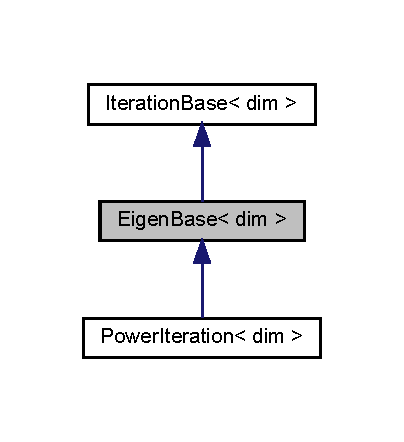
\includegraphics[width=194pt]{class_eigen_base__inherit__graph}
\end{center}
\end{figure}


Collaboration diagram for Eigen\+Base$<$ dim $>$\+:\nopagebreak
\begin{figure}[H]
\begin{center}
\leavevmode
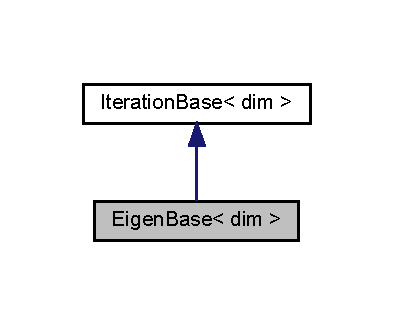
\includegraphics[width=189pt]{class_eigen_base__coll__graph}
\end{center}
\end{figure}
\subsection*{Public Member Functions}
\begin{DoxyCompactItemize}
\item 
\hyperlink{class_eigen_base_a041823ed11437980ff73ada87a9717fe}{Eigen\+Base} (const Parameter\+Handler \&prm)
\item 
virtual \hyperlink{class_eigen_base_afe9efbe26f3d5a427caa1d5022555038}{$\sim$\+Eigen\+Base} ()
\item 
virtual void \hyperlink{class_eigen_base_a8a9ef8878e5b7199aa662f2b61b2d864}{do\+\_\+iterations} (std\+::vector$<$ Vector$<$ double $>$ $>$ \&sflxes\+\_\+proc, std\+::vector$<$ std\+\_\+cxx11\+::shared\+\_\+ptr$<$ \hyperlink{class_equation_base}{Equation\+Base}$<$ dim $>$ $>$ $>$ \&equ\+\_\+ptrs, std\+\_\+cxx11\+::shared\+\_\+ptr$<$ \hyperlink{class_i_g_base}{I\+G\+Base}$<$ dim $>$ $>$ ig\+\_\+ptr, std\+\_\+cxx11\+::shared\+\_\+ptr$<$ \hyperlink{class_m_g_base}{M\+G\+Base}$<$ dim $>$ $>$ mg\+\_\+ptr)
\item 
virtual void \hyperlink{class_eigen_base_ae09830ed4bcb14b7b699cd5f5460fab7}{eigen\+\_\+iterations} (std\+::vector$<$ Vector$<$ double $>$ $>$ \&sflxes\+\_\+proc, std\+::vector$<$ std\+\_\+cxx11\+::shared\+\_\+ptr$<$ \hyperlink{class_equation_base}{Equation\+Base}$<$ dim $>$ $>$ $>$ \&equ\+\_\+ptrs, std\+\_\+cxx11\+::shared\+\_\+ptr$<$ \hyperlink{class_i_g_base}{I\+G\+Base}$<$ dim $>$ $>$ ig\+\_\+ptr, std\+\_\+cxx11\+::shared\+\_\+ptr$<$ \hyperlink{class_m_g_base}{M\+G\+Base}$<$ dim $>$ $>$ mg\+\_\+ptr)
\item 
virtual void \hyperlink{class_eigen_base_aa51c202e12e88c70652aefbe4d399f2b}{update\+\_\+prev\+\_\+sflxes\+\_\+fiss\+\_\+src\+\_\+keff} (std\+::vector$<$ Vector$<$ double $>$ $>$ \&sflxes\+\_\+proc)
\item 
double \hyperlink{class_eigen_base_a00569bdce088f65f71f4c743c6ec6c9b}{get\+\_\+keff} ()
\end{DoxyCompactItemize}
\subsection*{Protected Member Functions}
\begin{DoxyCompactItemize}
\item 
void \hyperlink{class_eigen_base_a982ceb033a4452633c612491544ab100}{initialize\+\_\+fiss\+\_\+process} (std\+::vector$<$ Vector$<$ double $>$ $>$ \&sflxes\+\_\+proc, std\+\_\+cxx11\+::shared\+\_\+ptr$<$ \hyperlink{class_equation_base}{Equation\+Base}$<$ dim $>$ $>$ \&equ\+\_\+ptr)
\item 
void \hyperlink{class_eigen_base_a325ceda011337e2416cef726bbd5d28f}{calculate\+\_\+fiss\+\_\+src\+\_\+keff} (std\+::vector$<$ Vector$<$ double $>$ $>$ \&sflxes\+\_\+proc, std\+\_\+cxx11\+::shared\+\_\+ptr$<$ \hyperlink{class_equation_base}{Equation\+Base}$<$ dim $>$ $>$ equ\+\_\+ptr)
\item 
double \hyperlink{class_eigen_base_a1ad5ce67d3534960731d34691db2f4d9}{estimate\+\_\+k} ()
\item 
double \hyperlink{class_eigen_base_ac9b7836c98e95a8be4d57b3ccf11f185}{estimate\+\_\+k\+\_\+diff} ()
\end{DoxyCompactItemize}
\subsection*{Protected Attributes}
\begin{DoxyCompactItemize}
\item 
const double \hyperlink{class_eigen_base_af082247a6dec17c46fd664a780d9a765}{err\+\_\+k\+\_\+tol}
\begin{DoxyCompactList}\small\item\em Tolerance for convergence check on $k_\mathrm{eff}$. \end{DoxyCompactList}\item 
const double \hyperlink{class_eigen_base_acc8e2b79484a329d746a55ba656feead}{err\+\_\+phi\+\_\+tol}
\begin{DoxyCompactList}\small\item\em Tolerance for convergence check on $\phi$. \end{DoxyCompactList}\item 
double \hyperlink{class_eigen_base_a9373e0bd7462b70829d88b82cb66ac10}{keff}
\begin{DoxyCompactList}\small\item\em $k_\mathrm{eff}$ value. \end{DoxyCompactList}\item 
double \hyperlink{class_eigen_base_a1499f0cb877e5dff2013328e06a29b4a}{keff\+\_\+prev}
\begin{DoxyCompactList}\small\item\em $k_\mathrm{eff}$ value from previous eigen iteration. \end{DoxyCompactList}\item 
double \hyperlink{class_eigen_base_a6fa0753510038439c30de5c1832e4ebc}{fiss\+\_\+src}
\begin{DoxyCompactList}\small\item\em Fission source. \end{DoxyCompactList}\item 
double \hyperlink{class_eigen_base_aa324e40bd20edd51659416da3220d295}{fiss\+\_\+src\+\_\+prev}
\begin{DoxyCompactList}\small\item\em Fission source from previous eigen iteration. \end{DoxyCompactList}\item 
std\+::vector$<$ Vector$<$ double $>$ $>$ \hyperlink{class_eigen_base_aec9885df50ea40a18fd5708061139843}{sflxes\+\_\+proc\+\_\+prev\+\_\+eigen}
\begin{DoxyCompactList}\small\item\em $\phi$ from previous eigen iteration for all groups \end{DoxyCompactList}\end{DoxyCompactItemize}


\subsection{Detailed Description}
\subsubsection*{template$<$int dim$>$\newline
class Eigen\+Base$<$ dim $>$}

This class provides eigenvalue calculations foundations. 

This class is the base class of eigenvalue calculations. It will operate the iteration at a high level without touching specifics in the equations. Alternatively, it interfaces with M\+G\+Base objects iteratively.

\begin{DoxyAuthor}{Author}
Weixiong Zheng 
\end{DoxyAuthor}
\begin{DoxyDate}{Date}
2017/09 
\end{DoxyDate}


Definition at line 19 of file eigen\+\_\+base.\+h.



\subsection{Constructor \& Destructor Documentation}
\mbox{\Hypertarget{class_eigen_base_a041823ed11437980ff73ada87a9717fe}\label{class_eigen_base_a041823ed11437980ff73ada87a9717fe}} 
\index{Eigen\+Base@{Eigen\+Base}!Eigen\+Base@{Eigen\+Base}}
\index{Eigen\+Base@{Eigen\+Base}!Eigen\+Base@{Eigen\+Base}}
\subsubsection{\texorpdfstring{Eigen\+Base()}{EigenBase()}}
{\footnotesize\ttfamily template$<$int dim$>$ \\
\hyperlink{class_eigen_base}{Eigen\+Base}$<$ dim $>$\+::\hyperlink{class_eigen_base}{Eigen\+Base} (\begin{DoxyParamCaption}\item[{const Parameter\+Handler \&}]{prm }\end{DoxyParamCaption})}



Definition at line 4 of file eigen\+\_\+base.\+cc.

\mbox{\Hypertarget{class_eigen_base_afe9efbe26f3d5a427caa1d5022555038}\label{class_eigen_base_afe9efbe26f3d5a427caa1d5022555038}} 
\index{Eigen\+Base@{Eigen\+Base}!````~Eigen\+Base@{$\sim$\+Eigen\+Base}}
\index{````~Eigen\+Base@{$\sim$\+Eigen\+Base}!Eigen\+Base@{Eigen\+Base}}
\subsubsection{\texorpdfstring{$\sim$\+Eigen\+Base()}{~EigenBase()}}
{\footnotesize\ttfamily template$<$int dim$>$ \\
\hyperlink{class_eigen_base}{Eigen\+Base}$<$ dim $>$\+::$\sim$\hyperlink{class_eigen_base}{Eigen\+Base} (\begin{DoxyParamCaption}{ }\end{DoxyParamCaption})\hspace{0.3cm}{\ttfamily [virtual]}}



Definition at line 14 of file eigen\+\_\+base.\+cc.



\subsection{Member Function Documentation}
\mbox{\Hypertarget{class_eigen_base_a325ceda011337e2416cef726bbd5d28f}\label{class_eigen_base_a325ceda011337e2416cef726bbd5d28f}} 
\index{Eigen\+Base@{Eigen\+Base}!calculate\+\_\+fiss\+\_\+src\+\_\+keff@{calculate\+\_\+fiss\+\_\+src\+\_\+keff}}
\index{calculate\+\_\+fiss\+\_\+src\+\_\+keff@{calculate\+\_\+fiss\+\_\+src\+\_\+keff}!Eigen\+Base@{Eigen\+Base}}
\subsubsection{\texorpdfstring{calculate\+\_\+fiss\+\_\+src\+\_\+keff()}{calculate\_fiss\_src\_keff()}}
{\footnotesize\ttfamily template$<$int dim$>$ \\
void \hyperlink{class_eigen_base}{Eigen\+Base}$<$ dim $>$\+::calculate\+\_\+fiss\+\_\+src\+\_\+keff (\begin{DoxyParamCaption}\item[{std\+::vector$<$ Vector$<$ double $>$ $>$ \&}]{sflxes\+\_\+proc,  }\item[{std\+\_\+cxx11\+::shared\+\_\+ptr$<$ \hyperlink{class_equation_base}{Equation\+Base}$<$ dim $>$ $>$}]{equ\+\_\+ptr }\end{DoxyParamCaption})\hspace{0.3cm}{\ttfamily [protected]}}

Function to estimate fission source and $k_\mathrm{eff}$ values.


\begin{DoxyParams}{Parameters}
{\em sflxes\+\_\+proc} & \\
\hline
\end{DoxyParams}
\begin{DoxyReturn}{Returns}
Void. 
\end{DoxyReturn}


Definition at line 72 of file eigen\+\_\+base.\+cc.

\mbox{\Hypertarget{class_eigen_base_a8a9ef8878e5b7199aa662f2b61b2d864}\label{class_eigen_base_a8a9ef8878e5b7199aa662f2b61b2d864}} 
\index{Eigen\+Base@{Eigen\+Base}!do\+\_\+iterations@{do\+\_\+iterations}}
\index{do\+\_\+iterations@{do\+\_\+iterations}!Eigen\+Base@{Eigen\+Base}}
\subsubsection{\texorpdfstring{do\+\_\+iterations()}{do\_iterations()}}
{\footnotesize\ttfamily template$<$int dim$>$ \\
void \hyperlink{class_eigen_base}{Eigen\+Base}$<$ dim $>$\+::do\+\_\+iterations (\begin{DoxyParamCaption}\item[{std\+::vector$<$ Vector$<$ double $>$ $>$ \&}]{sflxes\+\_\+proc,  }\item[{std\+::vector$<$ std\+\_\+cxx11\+::shared\+\_\+ptr$<$ \hyperlink{class_equation_base}{Equation\+Base}$<$ dim $>$ $>$ $>$ \&}]{equ\+\_\+ptrs,  }\item[{std\+\_\+cxx11\+::shared\+\_\+ptr$<$ \hyperlink{class_i_g_base}{I\+G\+Base}$<$ dim $>$ $>$}]{ig\+\_\+ptr,  }\item[{std\+\_\+cxx11\+::shared\+\_\+ptr$<$ \hyperlink{class_m_g_base}{M\+G\+Base}$<$ dim $>$ $>$}]{mg\+\_\+ptr }\end{DoxyParamCaption})\hspace{0.3cm}{\ttfamily [virtual]}}

This function calls eigen\+\_\+iterations to performs eigenvalue iterations.

\begin{DoxyRefDesc}{Todo}
\item[\hyperlink{todo__todo000002}{Todo}]Add N\+DA functionality. \end{DoxyRefDesc}


Definition at line 20 of file eigen\+\_\+base.\+cc.

\mbox{\Hypertarget{class_eigen_base_ae09830ed4bcb14b7b699cd5f5460fab7}\label{class_eigen_base_ae09830ed4bcb14b7b699cd5f5460fab7}} 
\index{Eigen\+Base@{Eigen\+Base}!eigen\+\_\+iterations@{eigen\+\_\+iterations}}
\index{eigen\+\_\+iterations@{eigen\+\_\+iterations}!Eigen\+Base@{Eigen\+Base}}
\subsubsection{\texorpdfstring{eigen\+\_\+iterations()}{eigen\_iterations()}}
{\footnotesize\ttfamily template$<$int dim$>$ \\
void \hyperlink{class_eigen_base}{Eigen\+Base}$<$ dim $>$\+::eigen\+\_\+iterations (\begin{DoxyParamCaption}\item[{std\+::vector$<$ Vector$<$ double $>$ $>$ \&}]{sflxes\+\_\+proc,  }\item[{std\+::vector$<$ std\+\_\+cxx11\+::shared\+\_\+ptr$<$ \hyperlink{class_equation_base}{Equation\+Base}$<$ dim $>$ $>$ $>$ \&}]{equ\+\_\+ptrs,  }\item[{std\+\_\+cxx11\+::shared\+\_\+ptr$<$ \hyperlink{class_i_g_base}{I\+G\+Base}$<$ dim $>$ $>$}]{ig\+\_\+ptr,  }\item[{std\+\_\+cxx11\+::shared\+\_\+ptr$<$ \hyperlink{class_m_g_base}{M\+G\+Base}$<$ dim $>$ $>$}]{mg\+\_\+ptr }\end{DoxyParamCaption})\hspace{0.3cm}{\ttfamily [virtual]}}

This virtual function performs eigenvalue iteration after overriding with the std\+::vector$<$std\+\_\+cxx11\+::shared\+\_\+ptr$<$Equation\+Base$<$dim$>$ $>$ $>$back().

\begin{DoxyReturn}{Returns}
Void. 
\end{DoxyReturn}


Reimplemented in \hyperlink{class_power_iteration_a583586002126f8b7a523e95327047cba}{Power\+Iteration$<$ dim $>$}.



Definition at line 50 of file eigen\+\_\+base.\+cc.

\mbox{\Hypertarget{class_eigen_base_a1ad5ce67d3534960731d34691db2f4d9}\label{class_eigen_base_a1ad5ce67d3534960731d34691db2f4d9}} 
\index{Eigen\+Base@{Eigen\+Base}!estimate\+\_\+k@{estimate\+\_\+k}}
\index{estimate\+\_\+k@{estimate\+\_\+k}!Eigen\+Base@{Eigen\+Base}}
\subsubsection{\texorpdfstring{estimate\+\_\+k()}{estimate\_k()}}
{\footnotesize\ttfamily template$<$int dim$>$ \\
double \hyperlink{class_eigen_base}{Eigen\+Base}$<$ dim $>$\+::estimate\+\_\+k (\begin{DoxyParamCaption}{ }\end{DoxyParamCaption})\hspace{0.3cm}{\ttfamily [protected]}}

Function to calculate $k_\mathrm{eff}$.

\begin{DoxyReturn}{Returns}
$k_\mathrm{eff}$ value. 
\end{DoxyReturn}


Definition at line 80 of file eigen\+\_\+base.\+cc.

\mbox{\Hypertarget{class_eigen_base_ac9b7836c98e95a8be4d57b3ccf11f185}\label{class_eigen_base_ac9b7836c98e95a8be4d57b3ccf11f185}} 
\index{Eigen\+Base@{Eigen\+Base}!estimate\+\_\+k\+\_\+diff@{estimate\+\_\+k\+\_\+diff}}
\index{estimate\+\_\+k\+\_\+diff@{estimate\+\_\+k\+\_\+diff}!Eigen\+Base@{Eigen\+Base}}
\subsubsection{\texorpdfstring{estimate\+\_\+k\+\_\+diff()}{estimate\_k\_diff()}}
{\footnotesize\ttfamily template$<$int dim$>$ \\
double \hyperlink{class_eigen_base}{Eigen\+Base}$<$ dim $>$\+::estimate\+\_\+k\+\_\+diff (\begin{DoxyParamCaption}{ }\end{DoxyParamCaption})\hspace{0.3cm}{\ttfamily [protected]}}

Function to calculate difference between $k_\mathrm{eff}$ and $k_\mathrm{eff,\ prev}$.

\begin{DoxyReturn}{Returns}
The relative difference (double type). 
\end{DoxyReturn}


Definition at line 86 of file eigen\+\_\+base.\+cc.

\mbox{\Hypertarget{class_eigen_base_a00569bdce088f65f71f4c743c6ec6c9b}\label{class_eigen_base_a00569bdce088f65f71f4c743c6ec6c9b}} 
\index{Eigen\+Base@{Eigen\+Base}!get\+\_\+keff@{get\+\_\+keff}}
\index{get\+\_\+keff@{get\+\_\+keff}!Eigen\+Base@{Eigen\+Base}}
\subsubsection{\texorpdfstring{get\+\_\+keff()}{get\_keff()}}
{\footnotesize\ttfamily template$<$int dim$>$ \\
double \hyperlink{class_eigen_base}{Eigen\+Base}$<$ dim $>$\+::get\+\_\+keff (\begin{DoxyParamCaption}{ }\end{DoxyParamCaption})}

Function to get $k_\mathrm{eff}$ value from eigenvalue iterations.

\begin{DoxyReturn}{Returns}
$k_\mathrm{eff}$ value (double type). 
\end{DoxyReturn}


Definition at line 92 of file eigen\+\_\+base.\+cc.

\mbox{\Hypertarget{class_eigen_base_a982ceb033a4452633c612491544ab100}\label{class_eigen_base_a982ceb033a4452633c612491544ab100}} 
\index{Eigen\+Base@{Eigen\+Base}!initialize\+\_\+fiss\+\_\+process@{initialize\+\_\+fiss\+\_\+process}}
\index{initialize\+\_\+fiss\+\_\+process@{initialize\+\_\+fiss\+\_\+process}!Eigen\+Base@{Eigen\+Base}}
\subsubsection{\texorpdfstring{initialize\+\_\+fiss\+\_\+process()}{initialize\_fiss\_process()}}
{\footnotesize\ttfamily template$<$int dim$>$ \\
void \hyperlink{class_eigen_base}{Eigen\+Base}$<$ dim $>$\+::initialize\+\_\+fiss\+\_\+process (\begin{DoxyParamCaption}\item[{std\+::vector$<$ Vector$<$ double $>$ $>$ \&}]{sflxes\+\_\+proc,  }\item[{std\+\_\+cxx11\+::shared\+\_\+ptr$<$ \hyperlink{class_equation_base}{Equation\+Base}$<$ dim $>$ $>$ \&}]{equ\+\_\+ptr }\end{DoxyParamCaption})\hspace{0.3cm}{\ttfamily [protected]}}

Function to initialize $k_\mathrm{eff}$ and fission source. $k_\mathrm{eff}$ is initilized with unit value while fission source is initialize with unit-\/value scalar fluxes for all groups.


\begin{DoxyParams}{Parameters}
{\em sflxes\+\_\+proc} & A vector of scalar fluxes of all groups living on current processor. \\
\hline
{\em equ\+\_\+ptr} & A pointer of Equation\+Base object. \\
\hline
\end{DoxyParams}
\begin{DoxyReturn}{Returns}
Void. 
\end{DoxyReturn}


Definition at line 38 of file eigen\+\_\+base.\+cc.

\mbox{\Hypertarget{class_eigen_base_aa51c202e12e88c70652aefbe4d399f2b}\label{class_eigen_base_aa51c202e12e88c70652aefbe4d399f2b}} 
\index{Eigen\+Base@{Eigen\+Base}!update\+\_\+prev\+\_\+sflxes\+\_\+fiss\+\_\+src\+\_\+keff@{update\+\_\+prev\+\_\+sflxes\+\_\+fiss\+\_\+src\+\_\+keff}}
\index{update\+\_\+prev\+\_\+sflxes\+\_\+fiss\+\_\+src\+\_\+keff@{update\+\_\+prev\+\_\+sflxes\+\_\+fiss\+\_\+src\+\_\+keff}!Eigen\+Base@{Eigen\+Base}}
\subsubsection{\texorpdfstring{update\+\_\+prev\+\_\+sflxes\+\_\+fiss\+\_\+src\+\_\+keff()}{update\_prev\_sflxes\_fiss\_src\_keff()}}
{\footnotesize\ttfamily template$<$int dim$>$ \\
void \hyperlink{class_eigen_base}{Eigen\+Base}$<$ dim $>$\+::update\+\_\+prev\+\_\+sflxes\+\_\+fiss\+\_\+src\+\_\+keff (\begin{DoxyParamCaption}\item[{std\+::vector$<$ Vector$<$ double $>$ $>$ \&}]{sflxes\+\_\+proc }\end{DoxyParamCaption})\hspace{0.3cm}{\ttfamily [virtual]}}

Function to update $\phi$, fission source and $k_\mathrm{eff}$ from previous iteration with current values.


\begin{DoxyParams}{Parameters}
{\em sflxes\+\_\+proc} & $\phi$ for all groups on current processor. \\
\hline
\end{DoxyParams}
\begin{DoxyReturn}{Returns}
Void 
\end{DoxyReturn}


Definition at line 59 of file eigen\+\_\+base.\+cc.



\subsection{Member Data Documentation}
\mbox{\Hypertarget{class_eigen_base_af082247a6dec17c46fd664a780d9a765}\label{class_eigen_base_af082247a6dec17c46fd664a780d9a765}} 
\index{Eigen\+Base@{Eigen\+Base}!err\+\_\+k\+\_\+tol@{err\+\_\+k\+\_\+tol}}
\index{err\+\_\+k\+\_\+tol@{err\+\_\+k\+\_\+tol}!Eigen\+Base@{Eigen\+Base}}
\subsubsection{\texorpdfstring{err\+\_\+k\+\_\+tol}{err\_k\_tol}}
{\footnotesize\ttfamily template$<$int dim$>$ \\
const double \hyperlink{class_eigen_base}{Eigen\+Base}$<$ dim $>$\+::err\+\_\+k\+\_\+tol\hspace{0.3cm}{\ttfamily [protected]}}



Tolerance for convergence check on $k_\mathrm{eff}$. 



Definition at line 105 of file eigen\+\_\+base.\+h.

\mbox{\Hypertarget{class_eigen_base_acc8e2b79484a329d746a55ba656feead}\label{class_eigen_base_acc8e2b79484a329d746a55ba656feead}} 
\index{Eigen\+Base@{Eigen\+Base}!err\+\_\+phi\+\_\+tol@{err\+\_\+phi\+\_\+tol}}
\index{err\+\_\+phi\+\_\+tol@{err\+\_\+phi\+\_\+tol}!Eigen\+Base@{Eigen\+Base}}
\subsubsection{\texorpdfstring{err\+\_\+phi\+\_\+tol}{err\_phi\_tol}}
{\footnotesize\ttfamily template$<$int dim$>$ \\
const double \hyperlink{class_eigen_base}{Eigen\+Base}$<$ dim $>$\+::err\+\_\+phi\+\_\+tol\hspace{0.3cm}{\ttfamily [protected]}}



Tolerance for convergence check on $\phi$. 



Definition at line 106 of file eigen\+\_\+base.\+h.

\mbox{\Hypertarget{class_eigen_base_a6fa0753510038439c30de5c1832e4ebc}\label{class_eigen_base_a6fa0753510038439c30de5c1832e4ebc}} 
\index{Eigen\+Base@{Eigen\+Base}!fiss\+\_\+src@{fiss\+\_\+src}}
\index{fiss\+\_\+src@{fiss\+\_\+src}!Eigen\+Base@{Eigen\+Base}}
\subsubsection{\texorpdfstring{fiss\+\_\+src}{fiss\_src}}
{\footnotesize\ttfamily template$<$int dim$>$ \\
double \hyperlink{class_eigen_base}{Eigen\+Base}$<$ dim $>$\+::fiss\+\_\+src\hspace{0.3cm}{\ttfamily [protected]}}



Fission source. 



Definition at line 110 of file eigen\+\_\+base.\+h.

\mbox{\Hypertarget{class_eigen_base_aa324e40bd20edd51659416da3220d295}\label{class_eigen_base_aa324e40bd20edd51659416da3220d295}} 
\index{Eigen\+Base@{Eigen\+Base}!fiss\+\_\+src\+\_\+prev@{fiss\+\_\+src\+\_\+prev}}
\index{fiss\+\_\+src\+\_\+prev@{fiss\+\_\+src\+\_\+prev}!Eigen\+Base@{Eigen\+Base}}
\subsubsection{\texorpdfstring{fiss\+\_\+src\+\_\+prev}{fiss\_src\_prev}}
{\footnotesize\ttfamily template$<$int dim$>$ \\
double \hyperlink{class_eigen_base}{Eigen\+Base}$<$ dim $>$\+::fiss\+\_\+src\+\_\+prev\hspace{0.3cm}{\ttfamily [protected]}}



Fission source from previous eigen iteration. 



Definition at line 111 of file eigen\+\_\+base.\+h.

\mbox{\Hypertarget{class_eigen_base_a9373e0bd7462b70829d88b82cb66ac10}\label{class_eigen_base_a9373e0bd7462b70829d88b82cb66ac10}} 
\index{Eigen\+Base@{Eigen\+Base}!keff@{keff}}
\index{keff@{keff}!Eigen\+Base@{Eigen\+Base}}
\subsubsection{\texorpdfstring{keff}{keff}}
{\footnotesize\ttfamily template$<$int dim$>$ \\
double \hyperlink{class_eigen_base}{Eigen\+Base}$<$ dim $>$\+::keff\hspace{0.3cm}{\ttfamily [protected]}}



$k_\mathrm{eff}$ value. 



Definition at line 108 of file eigen\+\_\+base.\+h.

\mbox{\Hypertarget{class_eigen_base_a1499f0cb877e5dff2013328e06a29b4a}\label{class_eigen_base_a1499f0cb877e5dff2013328e06a29b4a}} 
\index{Eigen\+Base@{Eigen\+Base}!keff\+\_\+prev@{keff\+\_\+prev}}
\index{keff\+\_\+prev@{keff\+\_\+prev}!Eigen\+Base@{Eigen\+Base}}
\subsubsection{\texorpdfstring{keff\+\_\+prev}{keff\_prev}}
{\footnotesize\ttfamily template$<$int dim$>$ \\
double \hyperlink{class_eigen_base}{Eigen\+Base}$<$ dim $>$\+::keff\+\_\+prev\hspace{0.3cm}{\ttfamily [protected]}}



$k_\mathrm{eff}$ value from previous eigen iteration. 



Definition at line 109 of file eigen\+\_\+base.\+h.

\mbox{\Hypertarget{class_eigen_base_aec9885df50ea40a18fd5708061139843}\label{class_eigen_base_aec9885df50ea40a18fd5708061139843}} 
\index{Eigen\+Base@{Eigen\+Base}!sflxes\+\_\+proc\+\_\+prev\+\_\+eigen@{sflxes\+\_\+proc\+\_\+prev\+\_\+eigen}}
\index{sflxes\+\_\+proc\+\_\+prev\+\_\+eigen@{sflxes\+\_\+proc\+\_\+prev\+\_\+eigen}!Eigen\+Base@{Eigen\+Base}}
\subsubsection{\texorpdfstring{sflxes\+\_\+proc\+\_\+prev\+\_\+eigen}{sflxes\_proc\_prev\_eigen}}
{\footnotesize\ttfamily template$<$int dim$>$ \\
std\+::vector$<$Vector$<$double$>$ $>$ \hyperlink{class_eigen_base}{Eigen\+Base}$<$ dim $>$\+::sflxes\+\_\+proc\+\_\+prev\+\_\+eigen\hspace{0.3cm}{\ttfamily [protected]}}



$\phi$ from previous eigen iteration for all groups 



Definition at line 114 of file eigen\+\_\+base.\+h.



The documentation for this class was generated from the following files\+:\begin{DoxyCompactItemize}
\item 
src/iteration/\hyperlink{eigen__base_8h}{eigen\+\_\+base.\+h}\item 
src/iteration/\hyperlink{eigen__base_8cc}{eigen\+\_\+base.\+cc}\end{DoxyCompactItemize}

\hypertarget{class_equation_base}{}\section{Equation\+Base$<$ dim $>$ Class Template Reference}
\label{class_equation_base}\index{Equation\+Base$<$ dim $>$@{Equation\+Base$<$ dim $>$}}


This class provides weak form assembly and physical quantity computation functionalities.  




{\ttfamily \#include $<$equation\+\_\+base.\+h$>$}



Inheritance diagram for Equation\+Base$<$ dim $>$\+:\nopagebreak
\begin{figure}[H]
\begin{center}
\leavevmode
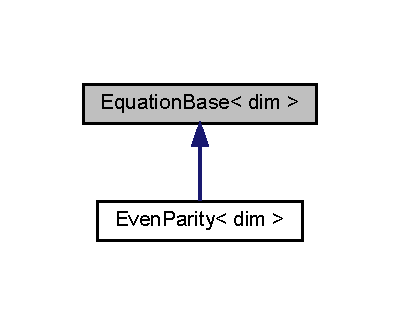
\includegraphics[width=192pt]{class_equation_base__inherit__graph}
\end{center}
\end{figure}
\subsection*{Public Member Functions}
\begin{DoxyCompactItemize}
\item 
\hyperlink{class_equation_base_a1e027696da2ab5a030daa34bf99430fe}{Equation\+Base} (std\+::string \hyperlink{class_equation_base_a0a72472959e531f5256400dec911f3a5}{equation\+\_\+name}, const Parameter\+Handler \&prm, const std\+\_\+cxx11\+::shared\+\_\+ptr$<$ \hyperlink{class_mesh_generator}{Mesh\+Generator}$<$ dim $>$ $>$ msh\+\_\+ptr, const std\+\_\+cxx11\+::shared\+\_\+ptr$<$ \hyperlink{class_a_q_base}{A\+Q\+Base}$<$ dim $>$ $>$ aqd\+\_\+ptr, const std\+\_\+cxx11\+::shared\+\_\+ptr$<$ \hyperlink{class_material_properties}{Material\+Properties} $>$ mat\+\_\+ptr)
\item 
virtual \hyperlink{class_equation_base_aee6cf5fc2a1580bb6070babdab0626ab}{$\sim$\+Equation\+Base} ()
\item 
virtual void \hyperlink{class_equation_base_a7d4047f59b31ef73ef404ab396712878}{assemble\+\_\+bilinear\+\_\+form} ()
\item 
virtual void \hyperlink{class_equation_base_a42472101cbaeab32d22c4e8ff1dc9830}{assemble\+\_\+volume\+\_\+boundary\+\_\+bilinear\+\_\+form} ()
\item 
virtual void \hyperlink{class_equation_base_ac590b2065d95ea03fcf411c965e6cfd9}{assemble\+\_\+interface\+\_\+bilinear\+\_\+form} ()
\begin{DoxyCompactList}\small\item\em Interface weak form assembly driver. Member function used to assemble interface weak forms. The main functionality is to go through all non-\/boundary interfaces of the cells owned on current processor and assemble the weak form using interface assembler. \end{DoxyCompactList}\item 
void \hyperlink{class_equation_base_a44faf34fc306d85f5e84e9c16bea985d}{assemble\+\_\+closure\+\_\+bilinear\+\_\+form} (std\+\_\+cxx11\+::shared\+\_\+ptr$<$ \hyperlink{class_equation_base}{Equation\+Base}$<$ dim $>$ $>$ ho\+\_\+equ\+\_\+ptr, bool do\+\_\+assembly=true)
\item 
virtual void \hyperlink{class_equation_base_ac08c0b8c03ccd29f0b9eb49f6e63f8e9}{assemble\+\_\+linear\+\_\+form} (std\+::vector$<$ Vector$<$ double $>$ $>$ \&sflx\+\_\+this\+\_\+proc, unsigned int \&g)
\item 
virtual void \hyperlink{class_equation_base_aa6a5d3dd752c1e2389b329c141c44ee7}{assemble\+\_\+fixed\+\_\+linear\+\_\+form} (std\+::vector$<$ Vector$<$ double $>$ $>$ \&sflx\+\_\+prev)
\item 
virtual void \hyperlink{class_equation_base_a39f0465a523e038302f624f89c08a2ee}{pre\+\_\+assemble\+\_\+cell\+\_\+matrices} (typename Do\+F\+Handler$<$ dim $>$\+::active\+\_\+cell\+\_\+iterator \&cell, std\+::vector$<$ std\+::vector$<$ Full\+Matrix$<$ double $>$ $>$ $>$ \&streaming\+\_\+at\+\_\+qp, std\+::vector$<$ Full\+Matrix$<$ double $>$ $>$ \&collision\+\_\+at\+\_\+qp)
\item 
virtual void \hyperlink{class_equation_base_a7421b3c18433975ac794ac22c3af715a}{integrate\+\_\+cell\+\_\+bilinear\+\_\+form} (typename Do\+F\+Handler$<$ dim $>$\+::active\+\_\+cell\+\_\+iterator \&cell, Full\+Matrix$<$ double $>$ \&cell\+\_\+matrix, std\+::vector$<$ std\+::vector$<$ Full\+Matrix$<$ double $>$ $>$ $>$ \&streaming\+\_\+at\+\_\+qp, std\+::vector$<$ Full\+Matrix$<$ double $>$ $>$ \&collision\+\_\+at\+\_\+qp, const unsigned int \&g, const unsigned int \&i\+\_\+dir)
\item 
virtual void \hyperlink{class_equation_base_ae294806284f671619cac9e7169ffff8d}{integrate\+\_\+boundary\+\_\+bilinear\+\_\+form} (typename Do\+F\+Handler$<$ dim $>$\+::active\+\_\+cell\+\_\+iterator \&cell, unsigned int \&fn, Full\+Matrix$<$ double $>$ \&cell\+\_\+matrix, const unsigned int \&g, const unsigned int \&i\+\_\+dir)
\begin{DoxyCompactList}\small\item\em Integrator for boundary weak form per boundary face per angular/group. \end{DoxyCompactList}\item 
virtual void \hyperlink{class_equation_base_af56caa04c80d8f388e116307930d0063}{integrate\+\_\+interface\+\_\+bilinear\+\_\+form} (typename Do\+F\+Handler$<$ dim $>$\+::active\+\_\+cell\+\_\+iterator \&cell, typename Do\+F\+Handler$<$ dim $>$\+::cell\+\_\+iterator \&neigh, unsigned int \&fn, Full\+Matrix$<$ double $>$ \&vi\+\_\+ui, Full\+Matrix$<$ double $>$ \&vi\+\_\+ue, Full\+Matrix$<$ double $>$ \&ve\+\_\+ui, Full\+Matrix$<$ double $>$ \&ve\+\_\+ue, const unsigned int \&g, const unsigned int \&i\+\_\+dir)
\begin{DoxyCompactList}\small\item\em Virtual function for interface integrator. When D\+F\+EM is used, this function can be overridden as interface weak form assembler per face per angular and group component. \end{DoxyCompactList}\item 
virtual void \hyperlink{class_equation_base_aca5998c1afd2b89ee93d3fbbfde7f3d0}{integrate\+\_\+scattering\+\_\+linear\+\_\+form} (typename Do\+F\+Handler$<$ dim $>$\+::active\+\_\+cell\+\_\+iterator \&cell, Vector$<$ double $>$ \&cell\+\_\+rhs, std\+::vector$<$ Vector$<$ double $>$ $>$ \&sflx\+\_\+proc, const unsigned int \&g, const unsigned int \&i\+\_\+dir)
\item 
virtual void \hyperlink{class_equation_base_ae8472f5c20d76c7d01e5660f8377887e}{integrate\+\_\+cell\+\_\+fixed\+\_\+linear\+\_\+form} (typename Do\+F\+Handler$<$ dim $>$\+::active\+\_\+cell\+\_\+iterator \&cell, Vector$<$ double $>$ \&cell\+\_\+rhs, std\+::vector$<$ Vector$<$ double $>$ $>$ \&sflx\+\_\+prev, const unsigned int \&g, const unsigned int \&i\+\_\+dir)
\item 
virtual void \hyperlink{class_equation_base_a1a213c4e21984bead9146e50be97077f}{integrate\+\_\+boundary\+\_\+linear\+\_\+form} (typename Do\+F\+Handler$<$ dim $>$\+::active\+\_\+cell\+\_\+iterator \&cell, unsigned int \&fn, Vector$<$ double $>$ \&cell\+\_\+rhses, const unsigned int \&g, const unsigned int \&i\+\_\+dir)
\begin{DoxyCompactList}\small\item\em Right hand side integrator specifically for boundary terms. \end{DoxyCompactList}\item 
virtual void \hyperlink{class_equation_base_a591282eb0ced01a7f22e29e7f0f44129}{solve\+\_\+in\+\_\+group} (const unsigned int \&g)
\item 
virtual void \hyperlink{class_equation_base_a25ff3b8e1a0c98dc5077e6afbac6606c}{initialize\+\_\+system\+\_\+matrices\+\_\+vectors} (Dynamic\+Sparsity\+Pattern \&dsp, Index\+Set \&local\+\_\+dofs, std\+::vector$<$ Vector$<$ double $>$ $>$ \&sflxes\+\_\+proc)
\item 
virtual void \hyperlink{class_equation_base_aa6ea21eec0c4e3e1dbb17da25b0633d3}{generate\+\_\+moments} (std\+::vector$<$ Vector$<$ double $>$ $>$ \&sflxes, std\+::vector$<$ Vector$<$ double $>$ $>$ \&sflxes\+\_\+old)
\item 
virtual void \hyperlink{class_equation_base_a893affe5706a8798bed68bb4ff531eec}{generate\+\_\+moments} (Vector$<$ double $>$ \&sflx, Vector$<$ double $>$ \&sflx\+\_\+old, const unsigned int \&g)
\item 
virtual void \hyperlink{class_equation_base_ab74a0a15d0d2a20022cafad8dd6f46aa}{generate\+\_\+moments} ()
\item 
virtual unsigned int \hyperlink{class_equation_base_a03a5a22088edb15689e0041dcc6d323c}{get\+\_\+component\+\_\+index} (unsigned int incident\+\_\+angle\+\_\+index, unsigned int g)
\item 
virtual unsigned int \hyperlink{class_equation_base_a4feaa86bdd6e84c4fc9195df67890c6a}{get\+\_\+component\+\_\+direction} (unsigned int comp\+\_\+ind)
\item 
virtual unsigned int \hyperlink{class_equation_base_a43a783f117149eac90a770d471cd7671}{get\+\_\+component\+\_\+group} (unsigned int comp\+\_\+ind)
\item 
double \hyperlink{class_equation_base_a1f36aebd8d54a082db3b2d2a621e67d6}{estimate\+\_\+fiss\+\_\+src} (std\+::vector$<$ Vector$<$ double $>$ $>$ \&sflxes\+\_\+proc)
\item 
void \hyperlink{class_equation_base_a4268bd83e1858fb6326c9b67851e85cc}{initialize\+\_\+cell\+\_\+iterators\+\_\+this\+\_\+proc} (const std\+\_\+cxx11\+::shared\+\_\+ptr$<$ \hyperlink{class_mesh_generator}{Mesh\+Generator}$<$ dim $>$ $>$ msh\+\_\+ptr, const Do\+F\+Handler$<$ dim $>$ \&dof\+\_\+handler)
\item 
void \hyperlink{class_equation_base_a932c91c91d2b758a155548e5b20ed1ff}{initialize\+\_\+assembly\+\_\+related\+\_\+objects} (F\+E\+\_\+\+Poly$<$ Tensor\+Product\+Polynomials$<$ dim $>$, dim, dim $>$ $\ast$fe)
\item 
void \hyperlink{class_equation_base_a13947db6be48085b9dca97117c73b5ca}{scale\+\_\+fiss\+\_\+transfer\+\_\+matrices} (double \hyperlink{class_equation_base_ab3cf94dc329f486555f89bdb0dd94ed6}{keff})
\item 
std\+::string \hyperlink{class_equation_base_abc4842a38ebb180b57ae11ec1325535c}{get\+\_\+equ\+\_\+name} ()
\end{DoxyCompactItemize}
\subsection*{Protected Member Functions}
\begin{DoxyCompactItemize}
\item 
unsigned int \hyperlink{class_equation_base_a7c46fc281a4040a89bbd97ccf0f46ac7}{get\+\_\+reflective\+\_\+direction\+\_\+index} (unsigned int boundary\+\_\+id, unsigned int incident\+\_\+angle\+\_\+index)
\end{DoxyCompactItemize}
\subsection*{Protected Attributes}
\begin{DoxyCompactItemize}
\item 
std\+\_\+cxx11\+::shared\+\_\+ptr$<$ Q\+Gauss$<$ dim $>$ $>$ \hyperlink{class_equation_base_a5e677b436f1abeeeffc3da284e5c1c4c}{q\+\_\+rule}
\begin{DoxyCompactList}\small\item\em $<$ Pointer of quadrature rule in cell. \end{DoxyCompactList}\item 
std\+\_\+cxx11\+::shared\+\_\+ptr$<$ Q\+Gauss$<$ dim-\/1 $>$ $>$ \hyperlink{class_equation_base_ab4c9256889d7f5a6b7d4295c81b9193b}{qf\+\_\+rule}
\begin{DoxyCompactList}\small\item\em Pointer of quadrature rule in cell for N\+DA correction term. \end{DoxyCompactList}\item 
std\+\_\+cxx11\+::shared\+\_\+ptr$<$ Q\+Gauss$<$ dim $>$ $>$ \hyperlink{class_equation_base_a306b0c876f50b5eb936e5bf71ebcd988}{qc\+\_\+rule}
\begin{DoxyCompactList}\small\item\em Pointer of quadrature rule on cell face for N\+DA correction term. \end{DoxyCompactList}\item 
std\+\_\+cxx11\+::shared\+\_\+ptr$<$ Q\+Gauss$<$ dim-\/1 $>$ $>$ \hyperlink{class_equation_base_a867f14c44c6132bd65542e9cdcf264c4}{qfc\+\_\+rule}
\item 
std\+\_\+cxx11\+::shared\+\_\+ptr$<$ F\+E\+Values$<$ dim $>$ $>$ \hyperlink{class_equation_base_abf3c19880eaea0911fff9eb7f3b4b425}{fv}
\begin{DoxyCompactList}\small\item\em Pointer of F\+E\+Values object. \end{DoxyCompactList}\item 
std\+\_\+cxx11\+::shared\+\_\+ptr$<$ F\+E\+Face\+Values$<$ dim $>$ $>$ \hyperlink{class_equation_base_a80b624dc27281e2758918d83fd38daf4}{fvf}
\item 
std\+\_\+cxx11\+::shared\+\_\+ptr$<$ F\+E\+Face\+Values$<$ dim $>$ $>$ \hyperlink{class_equation_base_abd53ef2bf719d3f8e72881072383180c}{fvf\+\_\+nei}
\item 
std\+\_\+cxx11\+::shared\+\_\+ptr$<$ F\+E\+Values$<$ dim $>$ $>$ \hyperlink{class_equation_base_a04c2626e352fcc6b1c24c50a7e899c2f}{fvc}
\item 
std\+\_\+cxx11\+::shared\+\_\+ptr$<$ F\+E\+Face\+Values$<$ dim $>$ $>$ \hyperlink{class_equation_base_a6f6ca8b0e78bcbe0edd07f7967a0a6f9}{fvfc}
\item 
std\+::string \hyperlink{class_equation_base_a0a72472959e531f5256400dec911f3a5}{equation\+\_\+name}
\begin{DoxyCompactList}\small\item\em String for equation name. \end{DoxyCompactList}\item 
std\+::string \hyperlink{class_equation_base_adf124367d26087d33b6f252aa3cdd0a3}{discretization}
\begin{DoxyCompactList}\small\item\em String for spatial discretization. \end{DoxyCompactList}\item 
double \hyperlink{class_equation_base_ab3cf94dc329f486555f89bdb0dd94ed6}{keff}
\begin{DoxyCompactList}\small\item\em keff with current generation of neutron. \end{DoxyCompactList}\item 
double \hyperlink{class_equation_base_a80de7bca9496a5739f842ed154ecd274}{keff\+\_\+prev\+\_\+gen}
\begin{DoxyCompactList}\small\item\em keff from last generation of neutron. \end{DoxyCompactList}\item 
double \hyperlink{class_equation_base_aec6881c5aa66a28deab370236219f569}{fission\+\_\+source}
\begin{DoxyCompactList}\small\item\em Fission source with current generation neutron. \end{DoxyCompactList}\item 
double \hyperlink{class_equation_base_aac7587c6cd96b508a52f1ed4782b4806}{fission\+\_\+source\+\_\+prev\+\_\+gen}
\begin{DoxyCompactList}\small\item\em Fission source with previous generation neutron. \end{DoxyCompactList}\item 
bool \hyperlink{class_equation_base_a749f717dadd0df287fd0c366a7a8e0c1}{is\+\_\+eigen\+\_\+problem}
\begin{DoxyCompactList}\small\item\em Boolean to determine if it\textquotesingle{}s eigenvalue problem. \end{DoxyCompactList}\item 
bool \hyperlink{class_equation_base_a908f21db148a15d7d51a8508aa1fc58a}{do\+\_\+nda}
\begin{DoxyCompactList}\small\item\em Boolean to determine if N\+DA is performed. \end{DoxyCompactList}\item 
bool \hyperlink{class_equation_base_a145ca193add91b43e7a00d6f35c0e1fb}{have\+\_\+reflective\+\_\+bc}
\begin{DoxyCompactList}\small\item\em Boolean to determine if problem has reflective BC. \end{DoxyCompactList}\item 
unsigned int \hyperlink{class_equation_base_a8b8a299e37005a06a089ace9f473f94e}{n\+\_\+q}
\begin{DoxyCompactList}\small\item\em Total number quadrature points in a cell for assembly. \end{DoxyCompactList}\item 
unsigned int \hyperlink{class_equation_base_ad0bad2bd155657e65a923910e5b114aa}{n\+\_\+qf}
\begin{DoxyCompactList}\small\item\em Total number of face quadrature points in face assembly. \end{DoxyCompactList}\item 
unsigned int \hyperlink{class_equation_base_a001c60e6c8df319b9f267688f84471da}{n\+\_\+qc}
\begin{DoxyCompactList}\small\item\em Total number of quadrature points for N\+DA correction assembly in cells. \end{DoxyCompactList}\item 
unsigned int \hyperlink{class_equation_base_a5cb013018da03250a101941f196df23b}{n\+\_\+qfc}
\begin{DoxyCompactList}\small\item\em Total number of quadrature points for N\+DA correction assembly on faces. \end{DoxyCompactList}\item 
unsigned int \hyperlink{class_equation_base_a66b4cac3e416505fba70789599a98d14}{dofs\+\_\+per\+\_\+cell}
\begin{DoxyCompactList}\small\item\em Total number of degrees of freedom per cell. \end{DoxyCompactList}\item 
unsigned int \hyperlink{class_equation_base_a7f01312245816bc60e1cf0a1630030a2}{n\+\_\+dir}
\begin{DoxyCompactList}\small\item\em Total number of directions if applicable. \end{DoxyCompactList}\item 
unsigned int \hyperlink{class_equation_base_a006861508fc71350aee8274fd949b1e6}{n\+\_\+azi}
\begin{DoxyCompactList}\small\item\em Total number of azimuthal angles if applicable. \end{DoxyCompactList}\item 
unsigned int \hyperlink{class_equation_base_a505c44d58215a614d263615a53159fda}{n\+\_\+total\+\_\+vars}
\begin{DoxyCompactList}\small\item\em Total number of components in current equation. \end{DoxyCompactList}\item 
unsigned int \hyperlink{class_equation_base_adf5fc09a70820108fd273b0e2183db55}{n\+\_\+group}
\begin{DoxyCompactList}\small\item\em Total number of groups. \end{DoxyCompactList}\item 
unsigned int \hyperlink{class_equation_base_a6eba5e7408331bce23945068cba4ed19}{n\+\_\+material}
\begin{DoxyCompactList}\small\item\em Total number of material types. \end{DoxyCompactList}\item 
unsigned int \hyperlink{class_equation_base_a0facd1cc5977e32b301a134ed5b9fa98}{p\+\_\+order}
\begin{DoxyCompactList}\small\item\em Polynomial order for finite elements. \end{DoxyCompactList}\item 
const unsigned int \hyperlink{class_equation_base_aafed438df52a6a2adca972fad322dd7b}{nda\+\_\+quadrature\+\_\+order}
\begin{DoxyCompactList}\small\item\em Quadrature order for N\+DA volumetric correction assembly. \end{DoxyCompactList}\item 
unsigned int \hyperlink{class_equation_base_a9433f3e6cb2251b0b7d0408570677b2e}{global\+\_\+refinements}
\item 
std\+::vector$<$ typename Do\+F\+Handler$<$ dim $>$\+::active\+\_\+cell\+\_\+iterator $>$ \hyperlink{class_equation_base_a60d687f69ae6fd56881c15435e91e4e5}{local\+\_\+cells}
\begin{DoxyCompactList}\small\item\em Number uniform refinements to perform. \end{DoxyCompactList}\item 
std\+::vector$<$ types\+::global\+\_\+dof\+\_\+index $>$ \hyperlink{class_equation_base_a63c4e27465bea3cf4c2348ea7f4782c8}{local\+\_\+dof\+\_\+indices}
\begin{DoxyCompactList}\small\item\em Local to global indices for all cells. \end{DoxyCompactList}\item 
std\+::vector$<$ types\+::global\+\_\+dof\+\_\+index $>$ \hyperlink{class_equation_base_a94114d6debfbf1955c3c39f5330ac3c2}{neigh\+\_\+dof\+\_\+indices}
\begin{DoxyCompactList}\small\item\em Local to global indices for all cells. \end{DoxyCompactList}\item 
std\+::vector$<$ Tensor$<$ 1, dim $>$ $>$ \hyperlink{class_equation_base_a46320b14358dd65c8450bba919c856d0}{omega\+\_\+i}
\begin{DoxyCompactList}\small\item\em All the directions. \end{DoxyCompactList}\item 
std\+::vector$<$ double $>$ \hyperlink{class_equation_base_a46388ad4bea156033fa98fd8f484a068}{wi}
\begin{DoxyCompactList}\small\item\em All the angular weight. \end{DoxyCompactList}\item 
std\+::vector$<$ std\+::vector$<$ double $>$ $>$ \hyperlink{class_equation_base_a818488c38892b44ccf25eb6f61e89ecc}{all\+\_\+sigt}
\begin{DoxyCompactList}\small\item\em $\sigma_\mathrm{t}$ of all groups for all materials. \end{DoxyCompactList}\item 
std\+::vector$<$ std\+::vector$<$ double $>$ $>$ \hyperlink{class_equation_base_aedead29f1c4bb6b9f7b17b1fe1441c5f}{all\+\_\+inv\+\_\+sigt}
\begin{DoxyCompactList}\small\item\em $1/\sigma_\mathrm{t}$ of all groups for all materials. \end{DoxyCompactList}\item 
std\+::vector$<$ std\+::vector$<$ double $>$ $>$ \hyperlink{class_equation_base_add5be1036bc07500adc0d925020798a6}{all\+\_\+q}
\begin{DoxyCompactList}\small\item\em $Q$ values of all groups for all materials. \end{DoxyCompactList}\item 
std\+::vector$<$ std\+::vector$<$ double $>$ $>$ \hyperlink{class_equation_base_a6a633374c56fe767325b5c0860269fbf}{all\+\_\+q\+\_\+per\+\_\+ster}
\begin{DoxyCompactList}\small\item\em $Q/(4\pi)$ values of all groups for all materials. \end{DoxyCompactList}\item 
std\+::vector$<$ std\+::vector$<$ double $>$ $>$ \hyperlink{class_equation_base_a8c88d4b3e532cb639cea6e653dee5cfc}{all\+\_\+nusigf}
\item 
std\+::vector$<$ std\+::vector$<$ std\+::vector$<$ double $>$ $>$ $>$ \hyperlink{class_equation_base_a6775388f6b8dcd903a0f95443b2e8c0d}{all\+\_\+sigs}
\item 
std\+::vector$<$ std\+::vector$<$ std\+::vector$<$ double $>$ $>$ $>$ \hyperlink{class_equation_base_abf2c1a575944b0661bb48e2380c269a0}{all\+\_\+sigs\+\_\+per\+\_\+ster}
\item 
std\+::vector$<$ std\+::vector$<$ std\+::vector$<$ double $>$ $>$ $>$ \hyperlink{class_equation_base_ab1bdb760ee1fb27a3e211f5dbdaef83d}{all\+\_\+chi\+\_\+nusigf}
\item 
std\+::vector$<$ std\+::vector$<$ std\+::vector$<$ double $>$ $>$ $>$ \hyperlink{class_equation_base_a98a7eeab206ded9b3444e074d1f89ea8}{all\+\_\+chi\+\_\+nusigf\+\_\+per\+\_\+ster}
\item 
std\+::vector$<$ std\+::vector$<$ std\+::vector$<$ double $>$ $>$ $>$ \hyperlink{class_equation_base_a5452991f01541261dba1e0322a0f5392}{scaled\+\_\+fiss\+\_\+transfer\+\_\+per\+\_\+ster}
\item 
std\+::vector$<$ std\+::vector$<$ std\+::vector$<$ double $>$ $>$ $>$ \hyperlink{class_equation_base_ad445f7f2e377cc05f2003de4d632baa7}{scat\+\_\+scaled\+\_\+fiss\+\_\+transfer\+\_\+per\+\_\+ster}
\item 
std\+::vector$<$ std\+::vector$<$ std\+::vector$<$ double $>$ $>$ $>$ \hyperlink{class_equation_base_aadf1651f816a1a65301faac3cd075aeb}{scaled\+\_\+fiss\+\_\+transfer}
\item 
std\+::map$<$ std\+::pair$<$ unsigned int, unsigned int $>$, unsigned int $>$ \hyperlink{class_equation_base_a7e2b3d305d1f1f7799acff6c86bc67f8}{component\+\_\+index}
\item 
std\+::map$<$ std\+::pair$<$ unsigned int, unsigned int $>$, unsigned int $>$ \hyperlink{class_equation_base_a55a37edb6a0cc2ac25e31b4e8aa91e33}{reflective\+\_\+direction\+\_\+index}
\item 
std\+::map$<$ std\+::vector$<$ unsigned int $>$, unsigned int $>$ \hyperlink{class_equation_base_a53b48062132ee777856a3b340b4000b2}{relative\+\_\+position\+\_\+to\+\_\+id}
\item 
std\+::unordered\+\_\+map$<$ unsigned int, std\+::pair$<$ unsigned int, unsigned int $>$ $>$ \hyperlink{class_equation_base_a1d2e520638913dfeb4e16f3a09911836}{inverse\+\_\+component\+\_\+index}
\item 
std\+::unordered\+\_\+map$<$ unsigned int, bool $>$ \hyperlink{class_equation_base_a91757532b2fd3759a976b22a83a9f8d8}{is\+\_\+reflective\+\_\+bc}
\item 
std\+::unordered\+\_\+map$<$ unsigned int, bool $>$ \hyperlink{class_equation_base_a2568ffad6a52d3bf3227eea51a314cb4}{is\+\_\+material\+\_\+fissile}
\item 
std\+::set$<$ unsigned int $>$ \hyperlink{class_equation_base_aafa902bf78cf78770557098fa9027188}{fissile\+\_\+ids}
\item 
Conditional\+O\+Stream \hyperlink{class_equation_base_a12dd28de05c41d4dd3ec30e7195bfa97}{pcout}
\end{DoxyCompactItemize}
\subsection*{Private Member Functions}
\begin{DoxyCompactItemize}
\item 
void \hyperlink{class_equation_base_afd853e7e9fd859216a705a517235c6ba}{process\+\_\+input} (const std\+\_\+cxx11\+::shared\+\_\+ptr$<$ \hyperlink{class_mesh_generator}{Mesh\+Generator}$<$ dim $>$ $>$ msh\+\_\+ptr, const std\+\_\+cxx11\+::shared\+\_\+ptr$<$ \hyperlink{class_a_q_base}{A\+Q\+Base}$<$ dim $>$ $>$ aqd\+\_\+ptr, const std\+\_\+cxx11\+::shared\+\_\+ptr$<$ \hyperlink{class_material_properties}{Material\+Properties} $>$ mat\+\_\+ptr)
\end{DoxyCompactItemize}
\subsection*{Private Attributes}
\begin{DoxyCompactItemize}
\item 
std\+\_\+cxx11\+::shared\+\_\+ptr$<$ \hyperlink{class_preconditioner_solver}{Preconditioner\+Solver} $>$ \hyperlink{class_equation_base_aa4b83dfa34d4588cf3250a21ffc2e984}{alg\+\_\+ptr}
\item 
std\+::vector$<$ P\+E\+T\+Sc\+Wrappers\+::\+M\+P\+I\+::\+Sparse\+Matrix $\ast$ $>$ \hyperlink{class_equation_base_afcdb76718da046b950c466500de44a03}{sys\+\_\+mats}
\item 
std\+::vector$<$ P\+E\+T\+Sc\+Wrappers\+::\+M\+P\+I\+::\+Vector $\ast$ $>$ \hyperlink{class_equation_base_a89fe13a13fa7f46cc20bdab8a884216c}{sys\+\_\+rhses}
\item 
std\+::vector$<$ P\+E\+T\+Sc\+Wrappers\+::\+M\+P\+I\+::\+Vector $\ast$ $>$ \hyperlink{class_equation_base_a556e9d3b402dae0303e786e2ef38a29b}{sys\+\_\+fixed\+\_\+rhses}
\item 
std\+::vector$<$ P\+E\+T\+Sc\+Wrappers\+::\+M\+P\+I\+::\+Vector $\ast$ $>$ \hyperlink{class_equation_base_afe48e9f1d2f6b4f13cefe80d43d18300}{sys\+\_\+aflxes}
\item 
std\+::vector$<$ Vector$<$ double $>$ $>$ \hyperlink{class_equation_base_aa5a26770211dc6c8b2c17e35deffa60b}{aflxes\+\_\+proc}
\item 
std\+::vector$<$ Vector$<$ double $>$ $>$ \hyperlink{class_equation_base_a25123cf5f335e267799a52420396a276}{ho\+\_\+sflxes\+\_\+proc}
\end{DoxyCompactItemize}


\subsection{Detailed Description}
\subsubsection*{template$<$int dim$>$\newline
class Equation\+Base$<$ dim $>$}

This class provides weak form assembly and physical quantity computation functionalities. 

The governing equation can be presented as \[ \mathcal{T}\psi=\mathcal{S}\psi+\mathcal{F}\psi\ (\mathrm{or}\ \frac{Q}{4\pi}), \] where $\mathcal{T}$, $\mathcal{S}$, $\mathcal{F}$ and $Q$ are the transport operator (including streaming and collision), scattering operator, fission operator and fixed volumetric source, respectively.

This class implements abstract functionalities of matrix and vector assembly of weak formulation for the governing equation above with finite element method as well as physical quantity computations such as fission source and $k_\mathrm{eff}$. It serves as the base class for any equation involved in B\+A\+RT calculation.

\begin{DoxyAuthor}{Author}
Weixiong Zheng 
\end{DoxyAuthor}
\begin{DoxyDate}{Date}
2017/06$\sim$08 
\end{DoxyDate}


Definition at line 50 of file equation\+\_\+base.\+h.



\subsection{Constructor \& Destructor Documentation}
\mbox{\Hypertarget{class_equation_base_a1e027696da2ab5a030daa34bf99430fe}\label{class_equation_base_a1e027696da2ab5a030daa34bf99430fe}} 
\index{Equation\+Base@{Equation\+Base}!Equation\+Base@{Equation\+Base}}
\index{Equation\+Base@{Equation\+Base}!Equation\+Base@{Equation\+Base}}
\subsubsection{\texorpdfstring{Equation\+Base()}{EquationBase()}}
{\footnotesize\ttfamily template$<$int dim$>$ \\
\hyperlink{class_equation_base}{Equation\+Base}$<$ dim $>$\+::\hyperlink{class_equation_base}{Equation\+Base} (\begin{DoxyParamCaption}\item[{std\+::string}]{equation\+\_\+name,  }\item[{const Parameter\+Handler \&}]{prm,  }\item[{const std\+\_\+cxx11\+::shared\+\_\+ptr$<$ \hyperlink{class_mesh_generator}{Mesh\+Generator}$<$ dim $>$ $>$}]{msh\+\_\+ptr,  }\item[{const std\+\_\+cxx11\+::shared\+\_\+ptr$<$ \hyperlink{class_a_q_base}{A\+Q\+Base}$<$ dim $>$ $>$}]{aqd\+\_\+ptr,  }\item[{const std\+\_\+cxx11\+::shared\+\_\+ptr$<$ \hyperlink{class_material_properties}{Material\+Properties} $>$}]{mat\+\_\+ptr }\end{DoxyParamCaption})}

Class constructor.


\begin{DoxyParams}{Parameters}
{\em equation\+\_\+name} & An abbreviated name of the equation. \\
\hline
{\em msh\+\_\+ptr} & An shared\+\_\+ptr of Mesh\+Generator$<$dim$>$ object. \\
\hline
{\em aqd\+\_\+ptr} & An shared\+\_\+ptr of A\+Q\+Base$<$dim$>$ object. \\
\hline
{\em mat\+\_\+ptr} & An shared\+\_\+ptr of Material\+Properties object. \\
\hline
\end{DoxyParams}


Definition at line 14 of file equation\+\_\+base.\+cc.

\mbox{\Hypertarget{class_equation_base_aee6cf5fc2a1580bb6070babdab0626ab}\label{class_equation_base_aee6cf5fc2a1580bb6070babdab0626ab}} 
\index{Equation\+Base@{Equation\+Base}!````~Equation\+Base@{$\sim$\+Equation\+Base}}
\index{````~Equation\+Base@{$\sim$\+Equation\+Base}!Equation\+Base@{Equation\+Base}}
\subsubsection{\texorpdfstring{$\sim$\+Equation\+Base()}{~EquationBase()}}
{\footnotesize\ttfamily template$<$int dim$>$ \\
\hyperlink{class_equation_base}{Equation\+Base}$<$ dim $>$\+::$\sim$\hyperlink{class_equation_base}{Equation\+Base} (\begin{DoxyParamCaption}{ }\end{DoxyParamCaption})\hspace{0.3cm}{\ttfamily [virtual]}}

Virtual class destructor. 

Definition at line 43 of file equation\+\_\+base.\+cc.



\subsection{Member Function Documentation}
\mbox{\Hypertarget{class_equation_base_a7d4047f59b31ef73ef404ab396712878}\label{class_equation_base_a7d4047f59b31ef73ef404ab396712878}} 
\index{Equation\+Base@{Equation\+Base}!assemble\+\_\+bilinear\+\_\+form@{assemble\+\_\+bilinear\+\_\+form}}
\index{assemble\+\_\+bilinear\+\_\+form@{assemble\+\_\+bilinear\+\_\+form}!Equation\+Base@{Equation\+Base}}
\subsubsection{\texorpdfstring{assemble\+\_\+bilinear\+\_\+form()}{assemble\_bilinear\_form()}}
{\footnotesize\ttfamily template$<$int dim$>$ \\
void \hyperlink{class_equation_base}{Equation\+Base}$<$ dim $>$\+::assemble\+\_\+bilinear\+\_\+form (\begin{DoxyParamCaption}{ }\end{DoxyParamCaption})\hspace{0.3cm}{\ttfamily [virtual]}}

Virtual function to assemble bilinear form. Inside this function, volumetric, boundary and cell interface (if applicable) bilinear forms will be assembled.

\begin{DoxyReturn}{Returns}
Void. 
\end{DoxyReturn}


Definition at line 191 of file equation\+\_\+base.\+cc.

\mbox{\Hypertarget{class_equation_base_a44faf34fc306d85f5e84e9c16bea985d}\label{class_equation_base_a44faf34fc306d85f5e84e9c16bea985d}} 
\index{Equation\+Base@{Equation\+Base}!assemble\+\_\+closure\+\_\+bilinear\+\_\+form@{assemble\+\_\+closure\+\_\+bilinear\+\_\+form}}
\index{assemble\+\_\+closure\+\_\+bilinear\+\_\+form@{assemble\+\_\+closure\+\_\+bilinear\+\_\+form}!Equation\+Base@{Equation\+Base}}
\subsubsection{\texorpdfstring{assemble\+\_\+closure\+\_\+bilinear\+\_\+form()}{assemble\_closure\_bilinear\_form()}}
{\footnotesize\ttfamily template$<$int dim$>$ \\
void \hyperlink{class_equation_base}{Equation\+Base}$<$ dim $>$\+::assemble\+\_\+closure\+\_\+bilinear\+\_\+form (\begin{DoxyParamCaption}\item[{std\+\_\+cxx11\+::shared\+\_\+ptr$<$ \hyperlink{class_equation_base}{Equation\+Base}$<$ dim $>$ $>$}]{ho\+\_\+equ\+\_\+ptr,  }\item[{bool}]{do\+\_\+assembly = {\ttfamily true} }\end{DoxyParamCaption})}



Definition at line 211 of file equation\+\_\+base.\+cc.

\mbox{\Hypertarget{class_equation_base_aa6a5d3dd752c1e2389b329c141c44ee7}\label{class_equation_base_aa6a5d3dd752c1e2389b329c141c44ee7}} 
\index{Equation\+Base@{Equation\+Base}!assemble\+\_\+fixed\+\_\+linear\+\_\+form@{assemble\+\_\+fixed\+\_\+linear\+\_\+form}}
\index{assemble\+\_\+fixed\+\_\+linear\+\_\+form@{assemble\+\_\+fixed\+\_\+linear\+\_\+form}!Equation\+Base@{Equation\+Base}}
\subsubsection{\texorpdfstring{assemble\+\_\+fixed\+\_\+linear\+\_\+form()}{assemble\_fixed\_linear\_form()}}
{\footnotesize\ttfamily template$<$int dim$>$ \\
void \hyperlink{class_equation_base}{Equation\+Base}$<$ dim $>$\+::assemble\+\_\+fixed\+\_\+linear\+\_\+form (\begin{DoxyParamCaption}\item[{std\+::vector$<$ Vector$<$ double $>$ $>$ \&}]{sflx\+\_\+prev }\end{DoxyParamCaption})\hspace{0.3cm}{\ttfamily [virtual]}}



Definition at line 589 of file equation\+\_\+base.\+cc.

\mbox{\Hypertarget{class_equation_base_ac590b2065d95ea03fcf411c965e6cfd9}\label{class_equation_base_ac590b2065d95ea03fcf411c965e6cfd9}} 
\index{Equation\+Base@{Equation\+Base}!assemble\+\_\+interface\+\_\+bilinear\+\_\+form@{assemble\+\_\+interface\+\_\+bilinear\+\_\+form}}
\index{assemble\+\_\+interface\+\_\+bilinear\+\_\+form@{assemble\+\_\+interface\+\_\+bilinear\+\_\+form}!Equation\+Base@{Equation\+Base}}
\subsubsection{\texorpdfstring{assemble\+\_\+interface\+\_\+bilinear\+\_\+form()}{assemble\_interface\_bilinear\_form()}}
{\footnotesize\ttfamily template$<$int dim$>$ \\
void \hyperlink{class_equation_base}{Equation\+Base}$<$ dim $>$\+::assemble\+\_\+interface\+\_\+bilinear\+\_\+form (\begin{DoxyParamCaption}{ }\end{DoxyParamCaption})\hspace{0.3cm}{\ttfamily [virtual]}}



Interface weak form assembly driver. Member function used to assemble interface weak forms. The main functionality is to go through all non-\/boundary interfaces of the cells owned on current processor and assemble the weak form using interface assembler. 

Virtual function to assemble interface bilinear form for D\+F\+EM. It is not recommended to override this function until there\textquotesingle{}s a strong reason. What it basically does is per component, we go over all cells on current processor and call integrators for cell interface bilinear form assembly.

\begin{DoxyNote}{Note}
Component loop needs to be the outer loop to avoid M\+PI related error caused by P\+E\+T\+Sc.
\end{DoxyNote}
\begin{DoxyReturn}{Returns}
void
\end{DoxyReturn}
There is no need to override this function for SN calculations. Yet, for PN, diffusion etc., this function must be overriden to correctly take care of the angular component. 

Definition at line 347 of file equation\+\_\+base.\+cc.

\mbox{\Hypertarget{class_equation_base_ac08c0b8c03ccd29f0b9eb49f6e63f8e9}\label{class_equation_base_ac08c0b8c03ccd29f0b9eb49f6e63f8e9}} 
\index{Equation\+Base@{Equation\+Base}!assemble\+\_\+linear\+\_\+form@{assemble\+\_\+linear\+\_\+form}}
\index{assemble\+\_\+linear\+\_\+form@{assemble\+\_\+linear\+\_\+form}!Equation\+Base@{Equation\+Base}}
\subsubsection{\texorpdfstring{assemble\+\_\+linear\+\_\+form()}{assemble\_linear\_form()}}
{\footnotesize\ttfamily template$<$int dim$>$ \\
void \hyperlink{class_equation_base}{Equation\+Base}$<$ dim $>$\+::assemble\+\_\+linear\+\_\+form (\begin{DoxyParamCaption}\item[{std\+::vector$<$ Vector$<$ double $>$ $>$ \&}]{sflx\+\_\+this\+\_\+proc,  }\item[{unsigned int \&}]{g }\end{DoxyParamCaption})\hspace{0.3cm}{\ttfamily [virtual]}}

Virtual function to assemble linear forms for a specific group using input flux. Overriding has to be provided. Preassumably, fission source or fixed source have been assembled before calling this function.

\begin{DoxyReturn}{Returns}
Void. 
\end{DoxyReturn}


Definition at line 545 of file equation\+\_\+base.\+cc.

\mbox{\Hypertarget{class_equation_base_a42472101cbaeab32d22c4e8ff1dc9830}\label{class_equation_base_a42472101cbaeab32d22c4e8ff1dc9830}} 
\index{Equation\+Base@{Equation\+Base}!assemble\+\_\+volume\+\_\+boundary\+\_\+bilinear\+\_\+form@{assemble\+\_\+volume\+\_\+boundary\+\_\+bilinear\+\_\+form}}
\index{assemble\+\_\+volume\+\_\+boundary\+\_\+bilinear\+\_\+form@{assemble\+\_\+volume\+\_\+boundary\+\_\+bilinear\+\_\+form}!Equation\+Base@{Equation\+Base}}
\subsubsection{\texorpdfstring{assemble\+\_\+volume\+\_\+boundary\+\_\+bilinear\+\_\+form()}{assemble\_volume\_boundary\_bilinear\_form()}}
{\footnotesize\ttfamily template$<$int dim$>$ \\
void \hyperlink{class_equation_base}{Equation\+Base}$<$ dim $>$\+::assemble\+\_\+volume\+\_\+boundary\+\_\+bilinear\+\_\+form (\begin{DoxyParamCaption}{ }\end{DoxyParamCaption})\hspace{0.3cm}{\ttfamily [virtual]}}

Virtual function to assemble volumetric and boundary bilinear form. It is not recommended to override this function until there\textquotesingle{}s a strong reason. What it basically does is per component, we go over all cells on current processor and call integrators for volumetric and boundary bilinear form assembly.

\begin{DoxyNote}{Note}
Component loop needs to be the outer loop to avoid M\+PI related error caused by P\+E\+T\+Sc.
\end{DoxyNote}
\begin{DoxyReturn}{Returns}
void 
\end{DoxyReturn}


Definition at line 225 of file equation\+\_\+base.\+cc.

\mbox{\Hypertarget{class_equation_base_a1f36aebd8d54a082db3b2d2a621e67d6}\label{class_equation_base_a1f36aebd8d54a082db3b2d2a621e67d6}} 
\index{Equation\+Base@{Equation\+Base}!estimate\+\_\+fiss\+\_\+src@{estimate\+\_\+fiss\+\_\+src}}
\index{estimate\+\_\+fiss\+\_\+src@{estimate\+\_\+fiss\+\_\+src}!Equation\+Base@{Equation\+Base}}
\subsubsection{\texorpdfstring{estimate\+\_\+fiss\+\_\+src()}{estimate\_fiss\_src()}}
{\footnotesize\ttfamily template$<$int dim$>$ \\
double \hyperlink{class_equation_base}{Equation\+Base}$<$ dim $>$\+::estimate\+\_\+fiss\+\_\+src (\begin{DoxyParamCaption}\item[{std\+::vector$<$ Vector$<$ double $>$ $>$ \&}]{sflxes\+\_\+proc }\end{DoxyParamCaption})}



Definition at line 636 of file equation\+\_\+base.\+cc.

\mbox{\Hypertarget{class_equation_base_aa6ea21eec0c4e3e1dbb17da25b0633d3}\label{class_equation_base_aa6ea21eec0c4e3e1dbb17da25b0633d3}} 
\index{Equation\+Base@{Equation\+Base}!generate\+\_\+moments@{generate\+\_\+moments}}
\index{generate\+\_\+moments@{generate\+\_\+moments}!Equation\+Base@{Equation\+Base}}
\subsubsection{\texorpdfstring{generate\+\_\+moments()}{generate\_moments()}\hspace{0.1cm}{\footnotesize\ttfamily [1/3]}}
{\footnotesize\ttfamily template$<$int dim$>$ \\
void \hyperlink{class_equation_base}{Equation\+Base}$<$ dim $>$\+::generate\+\_\+moments (\begin{DoxyParamCaption}\item[{std\+::vector$<$ Vector$<$ double $>$ $>$ \&}]{sflxes,  }\item[{std\+::vector$<$ Vector$<$ double $>$ $>$ \&}]{sflxes\+\_\+old }\end{DoxyParamCaption})\hspace{0.3cm}{\ttfamily [virtual]}}



Definition at line 461 of file equation\+\_\+base.\+cc.

\mbox{\Hypertarget{class_equation_base_a893affe5706a8798bed68bb4ff531eec}\label{class_equation_base_a893affe5706a8798bed68bb4ff531eec}} 
\index{Equation\+Base@{Equation\+Base}!generate\+\_\+moments@{generate\+\_\+moments}}
\index{generate\+\_\+moments@{generate\+\_\+moments}!Equation\+Base@{Equation\+Base}}
\subsubsection{\texorpdfstring{generate\+\_\+moments()}{generate\_moments()}\hspace{0.1cm}{\footnotesize\ttfamily [2/3]}}
{\footnotesize\ttfamily template$<$int dim$>$ \\
void \hyperlink{class_equation_base}{Equation\+Base}$<$ dim $>$\+::generate\+\_\+moments (\begin{DoxyParamCaption}\item[{Vector$<$ double $>$ \&}]{sflx,  }\item[{Vector$<$ double $>$ \&}]{sflx\+\_\+old,  }\item[{const unsigned int \&}]{g }\end{DoxyParamCaption})\hspace{0.3cm}{\ttfamily [virtual]}}



Definition at line 484 of file equation\+\_\+base.\+cc.

\mbox{\Hypertarget{class_equation_base_ab74a0a15d0d2a20022cafad8dd6f46aa}\label{class_equation_base_ab74a0a15d0d2a20022cafad8dd6f46aa}} 
\index{Equation\+Base@{Equation\+Base}!generate\+\_\+moments@{generate\+\_\+moments}}
\index{generate\+\_\+moments@{generate\+\_\+moments}!Equation\+Base@{Equation\+Base}}
\subsubsection{\texorpdfstring{generate\+\_\+moments()}{generate\_moments()}\hspace{0.1cm}{\footnotesize\ttfamily [3/3]}}
{\footnotesize\ttfamily template$<$int dim$>$ \\
void \hyperlink{class_equation_base}{Equation\+Base}$<$ dim $>$\+::generate\+\_\+moments (\begin{DoxyParamCaption}{ }\end{DoxyParamCaption})\hspace{0.3cm}{\ttfamily [virtual]}}



Definition at line 509 of file equation\+\_\+base.\+cc.

\mbox{\Hypertarget{class_equation_base_a4feaa86bdd6e84c4fc9195df67890c6a}\label{class_equation_base_a4feaa86bdd6e84c4fc9195df67890c6a}} 
\index{Equation\+Base@{Equation\+Base}!get\+\_\+component\+\_\+direction@{get\+\_\+component\+\_\+direction}}
\index{get\+\_\+component\+\_\+direction@{get\+\_\+component\+\_\+direction}!Equation\+Base@{Equation\+Base}}
\subsubsection{\texorpdfstring{get\+\_\+component\+\_\+direction()}{get\_component\_direction()}}
{\footnotesize\ttfamily template$<$int dim$>$ \\
unsigned int \hyperlink{class_equation_base}{Equation\+Base}$<$ dim $>$\+::get\+\_\+component\+\_\+direction (\begin{DoxyParamCaption}\item[{unsigned int}]{comp\+\_\+ind }\end{DoxyParamCaption})\hspace{0.3cm}{\ttfamily [virtual]}}



Definition at line 680 of file equation\+\_\+base.\+cc.

\mbox{\Hypertarget{class_equation_base_a43a783f117149eac90a770d471cd7671}\label{class_equation_base_a43a783f117149eac90a770d471cd7671}} 
\index{Equation\+Base@{Equation\+Base}!get\+\_\+component\+\_\+group@{get\+\_\+component\+\_\+group}}
\index{get\+\_\+component\+\_\+group@{get\+\_\+component\+\_\+group}!Equation\+Base@{Equation\+Base}}
\subsubsection{\texorpdfstring{get\+\_\+component\+\_\+group()}{get\_component\_group()}}
{\footnotesize\ttfamily template$<$int dim$>$ \\
unsigned int \hyperlink{class_equation_base}{Equation\+Base}$<$ dim $>$\+::get\+\_\+component\+\_\+group (\begin{DoxyParamCaption}\item[{unsigned int}]{comp\+\_\+ind }\end{DoxyParamCaption})\hspace{0.3cm}{\ttfamily [virtual]}}



Definition at line 686 of file equation\+\_\+base.\+cc.

\mbox{\Hypertarget{class_equation_base_a03a5a22088edb15689e0041dcc6d323c}\label{class_equation_base_a03a5a22088edb15689e0041dcc6d323c}} 
\index{Equation\+Base@{Equation\+Base}!get\+\_\+component\+\_\+index@{get\+\_\+component\+\_\+index}}
\index{get\+\_\+component\+\_\+index@{get\+\_\+component\+\_\+index}!Equation\+Base@{Equation\+Base}}
\subsubsection{\texorpdfstring{get\+\_\+component\+\_\+index()}{get\_component\_index()}}
{\footnotesize\ttfamily template$<$int dim$>$ \\
unsigned int \hyperlink{class_equation_base}{Equation\+Base}$<$ dim $>$\+::get\+\_\+component\+\_\+index (\begin{DoxyParamCaption}\item[{unsigned int}]{incident\+\_\+angle\+\_\+index,  }\item[{unsigned int}]{g }\end{DoxyParamCaption})\hspace{0.3cm}{\ttfamily [virtual]}}



Definition at line 672 of file equation\+\_\+base.\+cc.

\mbox{\Hypertarget{class_equation_base_abc4842a38ebb180b57ae11ec1325535c}\label{class_equation_base_abc4842a38ebb180b57ae11ec1325535c}} 
\index{Equation\+Base@{Equation\+Base}!get\+\_\+equ\+\_\+name@{get\+\_\+equ\+\_\+name}}
\index{get\+\_\+equ\+\_\+name@{get\+\_\+equ\+\_\+name}!Equation\+Base@{Equation\+Base}}
\subsubsection{\texorpdfstring{get\+\_\+equ\+\_\+name()}{get\_equ\_name()}}
{\footnotesize\ttfamily template$<$int dim$>$ \\
std\+::string \hyperlink{class_equation_base}{Equation\+Base}$<$ dim $>$\+::get\+\_\+equ\+\_\+name (\begin{DoxyParamCaption}{ }\end{DoxyParamCaption})}

Function to retrieve current equation name.

\begin{DoxyReturn}{Returns}
A string for the equation name. 
\end{DoxyReturn}


Definition at line 664 of file equation\+\_\+base.\+cc.

\mbox{\Hypertarget{class_equation_base_a7c46fc281a4040a89bbd97ccf0f46ac7}\label{class_equation_base_a7c46fc281a4040a89bbd97ccf0f46ac7}} 
\index{Equation\+Base@{Equation\+Base}!get\+\_\+reflective\+\_\+direction\+\_\+index@{get\+\_\+reflective\+\_\+direction\+\_\+index}}
\index{get\+\_\+reflective\+\_\+direction\+\_\+index@{get\+\_\+reflective\+\_\+direction\+\_\+index}!Equation\+Base@{Equation\+Base}}
\subsubsection{\texorpdfstring{get\+\_\+reflective\+\_\+direction\+\_\+index()}{get\_reflective\_direction\_index()}}
{\footnotesize\ttfamily template$<$int dim$>$ \\
unsigned int \hyperlink{class_equation_base}{Equation\+Base}$<$ dim $>$\+::get\+\_\+reflective\+\_\+direction\+\_\+index (\begin{DoxyParamCaption}\item[{unsigned int}]{boundary\+\_\+id,  }\item[{unsigned int}]{incident\+\_\+angle\+\_\+index }\end{DoxyParamCaption})\hspace{0.3cm}{\ttfamily [protected]}}

This function returns the mapping result\+: (boundary id, direction index)-\/$>$ refl. index.


\begin{DoxyParams}{Parameters}
{\em boundary\+\_\+id} & A integer representing ID of the boundary (ranging from 0 to 2$\ast$dim) \\
\hline
{\em incident\+\_\+angle\+\_\+index} & Incident direction index. \\
\hline
\end{DoxyParams}


Definition at line 693 of file equation\+\_\+base.\+cc.

\mbox{\Hypertarget{class_equation_base_a932c91c91d2b758a155548e5b20ed1ff}\label{class_equation_base_a932c91c91d2b758a155548e5b20ed1ff}} 
\index{Equation\+Base@{Equation\+Base}!initialize\+\_\+assembly\+\_\+related\+\_\+objects@{initialize\+\_\+assembly\+\_\+related\+\_\+objects}}
\index{initialize\+\_\+assembly\+\_\+related\+\_\+objects@{initialize\+\_\+assembly\+\_\+related\+\_\+objects}!Equation\+Base@{Equation\+Base}}
\subsubsection{\texorpdfstring{initialize\+\_\+assembly\+\_\+related\+\_\+objects()}{initialize\_assembly\_related\_objects()}}
{\footnotesize\ttfamily template$<$int dim$>$ \\
void \hyperlink{class_equation_base}{Equation\+Base}$<$ dim $>$\+::initialize\+\_\+assembly\+\_\+related\+\_\+objects (\begin{DoxyParamCaption}\item[{F\+E\+\_\+\+Poly$<$ Tensor\+Product\+Polynomials$<$ dim $>$, dim, dim $>$ $\ast$}]{fe }\end{DoxyParamCaption})}



Definition at line 139 of file equation\+\_\+base.\+cc.

\mbox{\Hypertarget{class_equation_base_a4268bd83e1858fb6326c9b67851e85cc}\label{class_equation_base_a4268bd83e1858fb6326c9b67851e85cc}} 
\index{Equation\+Base@{Equation\+Base}!initialize\+\_\+cell\+\_\+iterators\+\_\+this\+\_\+proc@{initialize\+\_\+cell\+\_\+iterators\+\_\+this\+\_\+proc}}
\index{initialize\+\_\+cell\+\_\+iterators\+\_\+this\+\_\+proc@{initialize\+\_\+cell\+\_\+iterators\+\_\+this\+\_\+proc}!Equation\+Base@{Equation\+Base}}
\subsubsection{\texorpdfstring{initialize\+\_\+cell\+\_\+iterators\+\_\+this\+\_\+proc()}{initialize\_cell\_iterators\_this\_proc()}}
{\footnotesize\ttfamily template$<$int dim$>$ \\
void \hyperlink{class_equation_base}{Equation\+Base}$<$ dim $>$\+::initialize\+\_\+cell\+\_\+iterators\+\_\+this\+\_\+proc (\begin{DoxyParamCaption}\item[{const std\+\_\+cxx11\+::shared\+\_\+ptr$<$ \hyperlink{class_mesh_generator}{Mesh\+Generator}$<$ dim $>$ $>$}]{msh\+\_\+ptr,  }\item[{const Do\+F\+Handler$<$ dim $>$ \&}]{dof\+\_\+handler }\end{DoxyParamCaption})}



Definition at line 100 of file equation\+\_\+base.\+cc.

\mbox{\Hypertarget{class_equation_base_a25ff3b8e1a0c98dc5077e6afbac6606c}\label{class_equation_base_a25ff3b8e1a0c98dc5077e6afbac6606c}} 
\index{Equation\+Base@{Equation\+Base}!initialize\+\_\+system\+\_\+matrices\+\_\+vectors@{initialize\+\_\+system\+\_\+matrices\+\_\+vectors}}
\index{initialize\+\_\+system\+\_\+matrices\+\_\+vectors@{initialize\+\_\+system\+\_\+matrices\+\_\+vectors}!Equation\+Base@{Equation\+Base}}
\subsubsection{\texorpdfstring{initialize\+\_\+system\+\_\+matrices\+\_\+vectors()}{initialize\_system\_matrices\_vectors()}}
{\footnotesize\ttfamily template$<$int dim$>$ \\
void \hyperlink{class_equation_base}{Equation\+Base}$<$ dim $>$\+::initialize\+\_\+system\+\_\+matrices\+\_\+vectors (\begin{DoxyParamCaption}\item[{Dynamic\+Sparsity\+Pattern \&}]{dsp,  }\item[{Index\+Set \&}]{local\+\_\+dofs,  }\item[{std\+::vector$<$ Vector$<$ double $>$ $>$ \&}]{sflxes\+\_\+proc }\end{DoxyParamCaption})\hspace{0.3cm}{\ttfamily [virtual]}}

Virtual function to initialize\+:

(1) Global matrices (P\+E\+T\+Sc objects) for all components;

(2) Global vectors (P\+E\+T\+Sc objects), i.\+e. solutions and right hand side vectors;

(3) $\phi$ for all groups living on current processor.


\begin{DoxyParams}{Parameters}
{\em dsp} & Sparsity pattern built from Bart\+Driver. \\
\hline
{\em local\+\_\+dofs} & Index set for indices of degrees of freedom living on current processor. \\
\hline
{\em sflxes\+\_\+proc} & $\phi$ for all groups on current processor. \\
\hline
\end{DoxyParams}


Definition at line 108 of file equation\+\_\+base.\+cc.

\mbox{\Hypertarget{class_equation_base_ae294806284f671619cac9e7169ffff8d}\label{class_equation_base_ae294806284f671619cac9e7169ffff8d}} 
\index{Equation\+Base@{Equation\+Base}!integrate\+\_\+boundary\+\_\+bilinear\+\_\+form@{integrate\+\_\+boundary\+\_\+bilinear\+\_\+form}}
\index{integrate\+\_\+boundary\+\_\+bilinear\+\_\+form@{integrate\+\_\+boundary\+\_\+bilinear\+\_\+form}!Equation\+Base@{Equation\+Base}}
\subsubsection{\texorpdfstring{integrate\+\_\+boundary\+\_\+bilinear\+\_\+form()}{integrate\_boundary\_bilinear\_form()}}
{\footnotesize\ttfamily template$<$int dim$>$ \\
void \hyperlink{class_equation_base}{Equation\+Base}$<$ dim $>$\+::integrate\+\_\+boundary\+\_\+bilinear\+\_\+form (\begin{DoxyParamCaption}\item[{typename Do\+F\+Handler$<$ dim $>$\+::active\+\_\+cell\+\_\+iterator \&}]{cell,  }\item[{unsigned int \&}]{fn,  }\item[{Full\+Matrix$<$ double $>$ \&}]{cell\+\_\+matrix,  }\item[{const unsigned int \&}]{g,  }\item[{const unsigned int \&}]{i\+\_\+dir }\end{DoxyParamCaption})\hspace{0.3cm}{\ttfamily [virtual]}}



Integrator for boundary weak form per boundary face per angular/group. 

The function is a virtual function. For diffusion-\/like system, i\+\_\+dir is set to 0 by default. 

Reimplemented in \hyperlink{class_even_parity_ae800cb49f85cf417167ca5385b50df6f}{Even\+Parity$<$ dim $>$}.



Definition at line 316 of file equation\+\_\+base.\+cc.

\mbox{\Hypertarget{class_equation_base_a1a213c4e21984bead9146e50be97077f}\label{class_equation_base_a1a213c4e21984bead9146e50be97077f}} 
\index{Equation\+Base@{Equation\+Base}!integrate\+\_\+boundary\+\_\+linear\+\_\+form@{integrate\+\_\+boundary\+\_\+linear\+\_\+form}}
\index{integrate\+\_\+boundary\+\_\+linear\+\_\+form@{integrate\+\_\+boundary\+\_\+linear\+\_\+form}!Equation\+Base@{Equation\+Base}}
\subsubsection{\texorpdfstring{integrate\+\_\+boundary\+\_\+linear\+\_\+form()}{integrate\_boundary\_linear\_form()}}
{\footnotesize\ttfamily template$<$int dim$>$ \\
void \hyperlink{class_equation_base}{Equation\+Base}$<$ dim $>$\+::integrate\+\_\+boundary\+\_\+linear\+\_\+form (\begin{DoxyParamCaption}\item[{typename Do\+F\+Handler$<$ dim $>$\+::active\+\_\+cell\+\_\+iterator \&}]{cell,  }\item[{unsigned int \&}]{fn,  }\item[{Vector$<$ double $>$ \&}]{cell\+\_\+rhses,  }\item[{const unsigned int \&}]{g,  }\item[{const unsigned int \&}]{i\+\_\+dir }\end{DoxyParamCaption})\hspace{0.3cm}{\ttfamily [virtual]}}



Right hand side integrator specifically for boundary terms. 



Definition at line 329 of file equation\+\_\+base.\+cc.

\mbox{\Hypertarget{class_equation_base_a7421b3c18433975ac794ac22c3af715a}\label{class_equation_base_a7421b3c18433975ac794ac22c3af715a}} 
\index{Equation\+Base@{Equation\+Base}!integrate\+\_\+cell\+\_\+bilinear\+\_\+form@{integrate\+\_\+cell\+\_\+bilinear\+\_\+form}}
\index{integrate\+\_\+cell\+\_\+bilinear\+\_\+form@{integrate\+\_\+cell\+\_\+bilinear\+\_\+form}!Equation\+Base@{Equation\+Base}}
\subsubsection{\texorpdfstring{integrate\+\_\+cell\+\_\+bilinear\+\_\+form()}{integrate\_cell\_bilinear\_form()}}
{\footnotesize\ttfamily template$<$int dim$>$ \\
void \hyperlink{class_equation_base}{Equation\+Base}$<$ dim $>$\+::integrate\+\_\+cell\+\_\+bilinear\+\_\+form (\begin{DoxyParamCaption}\item[{typename Do\+F\+Handler$<$ dim $>$\+::active\+\_\+cell\+\_\+iterator \&}]{cell,  }\item[{Full\+Matrix$<$ double $>$ \&}]{cell\+\_\+matrix,  }\item[{std\+::vector$<$ std\+::vector$<$ Full\+Matrix$<$ double $>$ $>$ $>$ \&}]{streaming\+\_\+at\+\_\+qp,  }\item[{std\+::vector$<$ Full\+Matrix$<$ double $>$ $>$ \&}]{collision\+\_\+at\+\_\+qp,  }\item[{const unsigned int \&}]{g,  }\item[{const unsigned int \&}]{i\+\_\+dir }\end{DoxyParamCaption})\hspace{0.3cm}{\ttfamily [virtual]}}

Virtual cell bilinear form integrator. 

Reimplemented in \hyperlink{class_even_parity_adb381ea4f45e5ae3741b1d30a0de02b6}{Even\+Parity$<$ dim $>$}.



Definition at line 300 of file equation\+\_\+base.\+cc.

\mbox{\Hypertarget{class_equation_base_ae8472f5c20d76c7d01e5660f8377887e}\label{class_equation_base_ae8472f5c20d76c7d01e5660f8377887e}} 
\index{Equation\+Base@{Equation\+Base}!integrate\+\_\+cell\+\_\+fixed\+\_\+linear\+\_\+form@{integrate\+\_\+cell\+\_\+fixed\+\_\+linear\+\_\+form}}
\index{integrate\+\_\+cell\+\_\+fixed\+\_\+linear\+\_\+form@{integrate\+\_\+cell\+\_\+fixed\+\_\+linear\+\_\+form}!Equation\+Base@{Equation\+Base}}
\subsubsection{\texorpdfstring{integrate\+\_\+cell\+\_\+fixed\+\_\+linear\+\_\+form()}{integrate\_cell\_fixed\_linear\_form()}}
{\footnotesize\ttfamily template$<$int dim$>$ \\
void \hyperlink{class_equation_base}{Equation\+Base}$<$ dim $>$\+::integrate\+\_\+cell\+\_\+fixed\+\_\+linear\+\_\+form (\begin{DoxyParamCaption}\item[{typename Do\+F\+Handler$<$ dim $>$\+::active\+\_\+cell\+\_\+iterator \&}]{cell,  }\item[{Vector$<$ double $>$ \&}]{cell\+\_\+rhs,  }\item[{std\+::vector$<$ Vector$<$ double $>$ $>$ \&}]{sflx\+\_\+prev,  }\item[{const unsigned int \&}]{g,  }\item[{const unsigned int \&}]{i\+\_\+dir }\end{DoxyParamCaption})\hspace{0.3cm}{\ttfamily [virtual]}}

Virtual function to provide cellwise integrator for linear form assembly specifically for the contribution of fixed source in fixed-\/source problems or fission in eigenvalue problems. It needs to be overriden for different derived classes. It can be represented with generic fission operator $\mathcal{F}$ as \[ \left(v,\mathcal{F}(\psi)\right)_\mathcal{D}, \]

where $v$, the test function, does not necessarily need to belong to the same function space as $\psi$.


\begin{DoxyParams}{Parameters}
{\em cell} & Active cell iterator containing cell info. \\
\hline
{\em cell\+\_\+rhs} & Local vector (linear form) to be modified. \\
\hline
{\em sflxes\+\_\+prev} & Scalar fluxes from previous generation due to fission for all groups living on current processor. \\
\hline
{\em g} & Group index. \\
\hline
{\em i\+\_\+dir} & Direction index. \\
\hline
\end{DoxyParams}
\begin{DoxyReturn}{Returns}
Void.
\end{DoxyReturn}
\begin{DoxyNote}{Note}
sflxes\+\_\+prev will do nothing inside the integrator fixed source problems. 
\end{DoxyNote}


Reimplemented in \hyperlink{class_even_parity_adc8fad33adf1fae4fb59268b365b21f9}{Even\+Parity$<$ dim $>$}.



Definition at line 613 of file equation\+\_\+base.\+cc.

\mbox{\Hypertarget{class_equation_base_af56caa04c80d8f388e116307930d0063}\label{class_equation_base_af56caa04c80d8f388e116307930d0063}} 
\index{Equation\+Base@{Equation\+Base}!integrate\+\_\+interface\+\_\+bilinear\+\_\+form@{integrate\+\_\+interface\+\_\+bilinear\+\_\+form}}
\index{integrate\+\_\+interface\+\_\+bilinear\+\_\+form@{integrate\+\_\+interface\+\_\+bilinear\+\_\+form}!Equation\+Base@{Equation\+Base}}
\subsubsection{\texorpdfstring{integrate\+\_\+interface\+\_\+bilinear\+\_\+form()}{integrate\_interface\_bilinear\_form()}}
{\footnotesize\ttfamily template$<$int dim$>$ \\
void \hyperlink{class_equation_base}{Equation\+Base}$<$ dim $>$\+::integrate\+\_\+interface\+\_\+bilinear\+\_\+form (\begin{DoxyParamCaption}\item[{typename Do\+F\+Handler$<$ dim $>$\+::active\+\_\+cell\+\_\+iterator \&}]{cell,  }\item[{typename Do\+F\+Handler$<$ dim $>$\+::cell\+\_\+iterator \&}]{neigh,  }\item[{unsigned int \&}]{fn,  }\item[{Full\+Matrix$<$ double $>$ \&}]{vi\+\_\+ui,  }\item[{Full\+Matrix$<$ double $>$ \&}]{vi\+\_\+ue,  }\item[{Full\+Matrix$<$ double $>$ \&}]{ve\+\_\+ui,  }\item[{Full\+Matrix$<$ double $>$ \&}]{ve\+\_\+ue,  }\item[{const unsigned int \&}]{g,  }\item[{const unsigned int \&}]{i\+\_\+dir }\end{DoxyParamCaption})\hspace{0.3cm}{\ttfamily [virtual]}}



Virtual function for interface integrator. When D\+F\+EM is used, this function can be overridden as interface weak form assembler per face per angular and group component. 

Virtual function provides integrator for interface bilinear form assembly in D\+F\+EM formulations. Mathematically, this contribute to the numerical flux term for D\+F\+EM. Generically, we would separate out four terms.


\begin{DoxyParams}{Parameters}
{\em cell} & Active cell iterator containing cell info. \\
\hline
{\em neigh} & Cell iterator for neighboring cell about current face. \\
\hline
{\em fn} & Face index in current cell for current boundary face. \\
\hline
{\em vi\+\_\+ui} & Face matrix from testing interior basis by interior basis. \\
\hline
{\em vi\+\_\+ue} & Face matrix from testing exterior basis by interior basis. \\
\hline
{\em ve\+\_\+ui} & Face matrix from testing interior basis by exterior basis. \\
\hline
{\em ve\+\_\+ue} & Face matrix from testing exterior basis by exterior basis. \\
\hline
{\em g} & Group index. \\
\hline
{\em i\+\_\+dir} & Direction index. \\
\hline
\end{DoxyParams}
\begin{DoxyReturn}{Returns}
Void.
\end{DoxyReturn}
When overridden for diffusion calculations, direction component is set to be zero by default 

Reimplemented in \hyperlink{class_even_parity_a0a6674c14f34f22c8ff383aee81ffabf}{Even\+Parity$<$ dim $>$}.



Definition at line 446 of file equation\+\_\+base.\+cc.

\mbox{\Hypertarget{class_equation_base_aca5998c1afd2b89ee93d3fbbfde7f3d0}\label{class_equation_base_aca5998c1afd2b89ee93d3fbbfde7f3d0}} 
\index{Equation\+Base@{Equation\+Base}!integrate\+\_\+scattering\+\_\+linear\+\_\+form@{integrate\+\_\+scattering\+\_\+linear\+\_\+form}}
\index{integrate\+\_\+scattering\+\_\+linear\+\_\+form@{integrate\+\_\+scattering\+\_\+linear\+\_\+form}!Equation\+Base@{Equation\+Base}}
\subsubsection{\texorpdfstring{integrate\+\_\+scattering\+\_\+linear\+\_\+form()}{integrate\_scattering\_linear\_form()}}
{\footnotesize\ttfamily template$<$int dim$>$ \\
void \hyperlink{class_equation_base}{Equation\+Base}$<$ dim $>$\+::integrate\+\_\+scattering\+\_\+linear\+\_\+form (\begin{DoxyParamCaption}\item[{typename Do\+F\+Handler$<$ dim $>$\+::active\+\_\+cell\+\_\+iterator \&}]{cell,  }\item[{Vector$<$ double $>$ \&}]{cell\+\_\+rhs,  }\item[{std\+::vector$<$ Vector$<$ double $>$ $>$ \&}]{sflx\+\_\+proc,  }\item[{const unsigned int \&}]{g,  }\item[{const unsigned int \&}]{i\+\_\+dir }\end{DoxyParamCaption})\hspace{0.3cm}{\ttfamily [virtual]}}

Virtual function to provide cellwise integrator for linear form assembly specifically for the contribution of scattering. It needs to be overriden for different derived classes.


\begin{DoxyParams}{Parameters}
{\em cell} & Active cell iterator containing cell info. \\
\hline
{\em cell\+\_\+rhs} & Local vector (linear form) to be modified. \\
\hline
{\em sflxes\+\_\+proc} & Scalar fluxes for all groups living on current processor. \\
\hline
{\em g} & Group index. \\
\hline
{\em i\+\_\+dir} & Direction index. \\
\hline
\end{DoxyParams}
\begin{DoxyReturn}{Returns}
Void. 
\end{DoxyReturn}


Reimplemented in \hyperlink{class_even_parity_ad29fd3a026508233ef772ea11f27402e}{Even\+Parity$<$ dim $>$}.



Definition at line 579 of file equation\+\_\+base.\+cc.

\mbox{\Hypertarget{class_equation_base_a39f0465a523e038302f624f89c08a2ee}\label{class_equation_base_a39f0465a523e038302f624f89c08a2ee}} 
\index{Equation\+Base@{Equation\+Base}!pre\+\_\+assemble\+\_\+cell\+\_\+matrices@{pre\+\_\+assemble\+\_\+cell\+\_\+matrices}}
\index{pre\+\_\+assemble\+\_\+cell\+\_\+matrices@{pre\+\_\+assemble\+\_\+cell\+\_\+matrices}!Equation\+Base@{Equation\+Base}}
\subsubsection{\texorpdfstring{pre\+\_\+assemble\+\_\+cell\+\_\+matrices()}{pre\_assemble\_cell\_matrices()}}
{\footnotesize\ttfamily template$<$int dim$>$ \\
void \hyperlink{class_equation_base}{Equation\+Base}$<$ dim $>$\+::pre\+\_\+assemble\+\_\+cell\+\_\+matrices (\begin{DoxyParamCaption}\item[{typename Do\+F\+Handler$<$ dim $>$\+::active\+\_\+cell\+\_\+iterator \&}]{cell,  }\item[{std\+::vector$<$ std\+::vector$<$ Full\+Matrix$<$ double $>$ $>$ $>$ \&}]{streaming\+\_\+at\+\_\+qp,  }\item[{std\+::vector$<$ Full\+Matrix$<$ double $>$ $>$ \&}]{collision\+\_\+at\+\_\+qp }\end{DoxyParamCaption})\hspace{0.3cm}{\ttfamily [virtual]}}



Reimplemented in \hyperlink{class_even_parity_a4cc64002161193e2227e962c9ecb8cf5}{Even\+Parity$<$ dim $>$}.



Definition at line 290 of file equation\+\_\+base.\+cc.

\mbox{\Hypertarget{class_equation_base_afd853e7e9fd859216a705a517235c6ba}\label{class_equation_base_afd853e7e9fd859216a705a517235c6ba}} 
\index{Equation\+Base@{Equation\+Base}!process\+\_\+input@{process\+\_\+input}}
\index{process\+\_\+input@{process\+\_\+input}!Equation\+Base@{Equation\+Base}}
\subsubsection{\texorpdfstring{process\+\_\+input()}{process\_input()}}
{\footnotesize\ttfamily template$<$int dim$>$ \\
void \hyperlink{class_equation_base}{Equation\+Base}$<$ dim $>$\+::process\+\_\+input (\begin{DoxyParamCaption}\item[{const std\+\_\+cxx11\+::shared\+\_\+ptr$<$ \hyperlink{class_mesh_generator}{Mesh\+Generator}$<$ dim $>$ $>$}]{msh\+\_\+ptr,  }\item[{const std\+\_\+cxx11\+::shared\+\_\+ptr$<$ \hyperlink{class_a_q_base}{A\+Q\+Base}$<$ dim $>$ $>$}]{aqd\+\_\+ptr,  }\item[{const std\+\_\+cxx11\+::shared\+\_\+ptr$<$ \hyperlink{class_material_properties}{Material\+Properties} $>$}]{mat\+\_\+ptr }\end{DoxyParamCaption})\hspace{0.3cm}{\ttfamily [private]}}



Definition at line 49 of file equation\+\_\+base.\+cc.

\mbox{\Hypertarget{class_equation_base_a13947db6be48085b9dca97117c73b5ca}\label{class_equation_base_a13947db6be48085b9dca97117c73b5ca}} 
\index{Equation\+Base@{Equation\+Base}!scale\+\_\+fiss\+\_\+transfer\+\_\+matrices@{scale\+\_\+fiss\+\_\+transfer\+\_\+matrices}}
\index{scale\+\_\+fiss\+\_\+transfer\+\_\+matrices@{scale\+\_\+fiss\+\_\+transfer\+\_\+matrices}!Equation\+Base@{Equation\+Base}}
\subsubsection{\texorpdfstring{scale\+\_\+fiss\+\_\+transfer\+\_\+matrices()}{scale\_fiss\_transfer\_matrices()}}
{\footnotesize\ttfamily template$<$int dim$>$ \\
void \hyperlink{class_equation_base}{Equation\+Base}$<$ dim $>$\+::scale\+\_\+fiss\+\_\+transfer\+\_\+matrices (\begin{DoxyParamCaption}\item[{double}]{keff }\end{DoxyParamCaption})}



Definition at line 526 of file equation\+\_\+base.\+cc.

\mbox{\Hypertarget{class_equation_base_a591282eb0ced01a7f22e29e7f0f44129}\label{class_equation_base_a591282eb0ced01a7f22e29e7f0f44129}} 
\index{Equation\+Base@{Equation\+Base}!solve\+\_\+in\+\_\+group@{solve\+\_\+in\+\_\+group}}
\index{solve\+\_\+in\+\_\+group@{solve\+\_\+in\+\_\+group}!Equation\+Base@{Equation\+Base}}
\subsubsection{\texorpdfstring{solve\+\_\+in\+\_\+group()}{solve\_in\_group()}}
{\footnotesize\ttfamily template$<$int dim$>$ \\
void \hyperlink{class_equation_base}{Equation\+Base}$<$ dim $>$\+::solve\+\_\+in\+\_\+group (\begin{DoxyParamCaption}\item[{const unsigned int \&}]{g }\end{DoxyParamCaption})\hspace{0.3cm}{\ttfamily [virtual]}}

Virtual function to perform one-\/pass linear solve for all components in target group. As diffusion has no concept of direction, this function has to be overriden in such a case. For SN, yet, no overriden is needed unless Krylov method is developed.


\begin{DoxyParams}{Parameters}
{\em g} & Group index. \\
\hline
\end{DoxyParams}


Definition at line 622 of file equation\+\_\+base.\+cc.



\subsection{Member Data Documentation}
\mbox{\Hypertarget{class_equation_base_aa5a26770211dc6c8b2c17e35deffa60b}\label{class_equation_base_aa5a26770211dc6c8b2c17e35deffa60b}} 
\index{Equation\+Base@{Equation\+Base}!aflxes\+\_\+proc@{aflxes\+\_\+proc}}
\index{aflxes\+\_\+proc@{aflxes\+\_\+proc}!Equation\+Base@{Equation\+Base}}
\subsubsection{\texorpdfstring{aflxes\+\_\+proc}{aflxes\_proc}}
{\footnotesize\ttfamily template$<$int dim$>$ \\
std\+::vector$<$Vector$<$double$>$ $>$ \hyperlink{class_equation_base}{Equation\+Base}$<$ dim $>$\+::aflxes\+\_\+proc\hspace{0.3cm}{\ttfamily [private]}}



Definition at line 431 of file equation\+\_\+base.\+h.

\mbox{\Hypertarget{class_equation_base_aa4b83dfa34d4588cf3250a21ffc2e984}\label{class_equation_base_aa4b83dfa34d4588cf3250a21ffc2e984}} 
\index{Equation\+Base@{Equation\+Base}!alg\+\_\+ptr@{alg\+\_\+ptr}}
\index{alg\+\_\+ptr@{alg\+\_\+ptr}!Equation\+Base@{Equation\+Base}}
\subsubsection{\texorpdfstring{alg\+\_\+ptr}{alg\_ptr}}
{\footnotesize\ttfamily template$<$int dim$>$ \\
std\+\_\+cxx11\+::shared\+\_\+ptr$<$\hyperlink{class_preconditioner_solver}{Preconditioner\+Solver}$>$ \hyperlink{class_equation_base}{Equation\+Base}$<$ dim $>$\+::alg\+\_\+ptr\hspace{0.3cm}{\ttfamily [private]}}



Definition at line 424 of file equation\+\_\+base.\+h.

\mbox{\Hypertarget{class_equation_base_ab1bdb760ee1fb27a3e211f5dbdaef83d}\label{class_equation_base_ab1bdb760ee1fb27a3e211f5dbdaef83d}} 
\index{Equation\+Base@{Equation\+Base}!all\+\_\+chi\+\_\+nusigf@{all\+\_\+chi\+\_\+nusigf}}
\index{all\+\_\+chi\+\_\+nusigf@{all\+\_\+chi\+\_\+nusigf}!Equation\+Base@{Equation\+Base}}
\subsubsection{\texorpdfstring{all\+\_\+chi\+\_\+nusigf}{all\_chi\_nusigf}}
{\footnotesize\ttfamily template$<$int dim$>$ \\
std\+::vector$<$std\+::vector$<$std\+::vector$<$double$>$ $>$ $>$ \hyperlink{class_equation_base}{Equation\+Base}$<$ dim $>$\+::all\+\_\+chi\+\_\+nusigf\hspace{0.3cm}{\ttfamily [protected]}}



Definition at line 403 of file equation\+\_\+base.\+h.

\mbox{\Hypertarget{class_equation_base_a98a7eeab206ded9b3444e074d1f89ea8}\label{class_equation_base_a98a7eeab206ded9b3444e074d1f89ea8}} 
\index{Equation\+Base@{Equation\+Base}!all\+\_\+chi\+\_\+nusigf\+\_\+per\+\_\+ster@{all\+\_\+chi\+\_\+nusigf\+\_\+per\+\_\+ster}}
\index{all\+\_\+chi\+\_\+nusigf\+\_\+per\+\_\+ster@{all\+\_\+chi\+\_\+nusigf\+\_\+per\+\_\+ster}!Equation\+Base@{Equation\+Base}}
\subsubsection{\texorpdfstring{all\+\_\+chi\+\_\+nusigf\+\_\+per\+\_\+ster}{all\_chi\_nusigf\_per\_ster}}
{\footnotesize\ttfamily template$<$int dim$>$ \\
std\+::vector$<$std\+::vector$<$std\+::vector$<$double$>$ $>$ $>$ \hyperlink{class_equation_base}{Equation\+Base}$<$ dim $>$\+::all\+\_\+chi\+\_\+nusigf\+\_\+per\+\_\+ster\hspace{0.3cm}{\ttfamily [protected]}}



Definition at line 404 of file equation\+\_\+base.\+h.

\mbox{\Hypertarget{class_equation_base_aedead29f1c4bb6b9f7b17b1fe1441c5f}\label{class_equation_base_aedead29f1c4bb6b9f7b17b1fe1441c5f}} 
\index{Equation\+Base@{Equation\+Base}!all\+\_\+inv\+\_\+sigt@{all\+\_\+inv\+\_\+sigt}}
\index{all\+\_\+inv\+\_\+sigt@{all\+\_\+inv\+\_\+sigt}!Equation\+Base@{Equation\+Base}}
\subsubsection{\texorpdfstring{all\+\_\+inv\+\_\+sigt}{all\_inv\_sigt}}
{\footnotesize\ttfamily template$<$int dim$>$ \\
std\+::vector$<$std\+::vector$<$double$>$ $>$ \hyperlink{class_equation_base}{Equation\+Base}$<$ dim $>$\+::all\+\_\+inv\+\_\+sigt\hspace{0.3cm}{\ttfamily [protected]}}



$1/\sigma_\mathrm{t}$ of all groups for all materials. 



Definition at line 393 of file equation\+\_\+base.\+h.

\mbox{\Hypertarget{class_equation_base_a8c88d4b3e532cb639cea6e653dee5cfc}\label{class_equation_base_a8c88d4b3e532cb639cea6e653dee5cfc}} 
\index{Equation\+Base@{Equation\+Base}!all\+\_\+nusigf@{all\+\_\+nusigf}}
\index{all\+\_\+nusigf@{all\+\_\+nusigf}!Equation\+Base@{Equation\+Base}}
\subsubsection{\texorpdfstring{all\+\_\+nusigf}{all\_nusigf}}
{\footnotesize\ttfamily template$<$int dim$>$ \\
std\+::vector$<$std\+::vector$<$double$>$ $>$ \hyperlink{class_equation_base}{Equation\+Base}$<$ dim $>$\+::all\+\_\+nusigf\hspace{0.3cm}{\ttfamily [protected]}}



Definition at line 400 of file equation\+\_\+base.\+h.

\mbox{\Hypertarget{class_equation_base_add5be1036bc07500adc0d925020798a6}\label{class_equation_base_add5be1036bc07500adc0d925020798a6}} 
\index{Equation\+Base@{Equation\+Base}!all\+\_\+q@{all\+\_\+q}}
\index{all\+\_\+q@{all\+\_\+q}!Equation\+Base@{Equation\+Base}}
\subsubsection{\texorpdfstring{all\+\_\+q}{all\_q}}
{\footnotesize\ttfamily template$<$int dim$>$ \\
std\+::vector$<$std\+::vector$<$double$>$ $>$ \hyperlink{class_equation_base}{Equation\+Base}$<$ dim $>$\+::all\+\_\+q\hspace{0.3cm}{\ttfamily [protected]}}



$Q$ values of all groups for all materials. 



Definition at line 396 of file equation\+\_\+base.\+h.

\mbox{\Hypertarget{class_equation_base_a6a633374c56fe767325b5c0860269fbf}\label{class_equation_base_a6a633374c56fe767325b5c0860269fbf}} 
\index{Equation\+Base@{Equation\+Base}!all\+\_\+q\+\_\+per\+\_\+ster@{all\+\_\+q\+\_\+per\+\_\+ster}}
\index{all\+\_\+q\+\_\+per\+\_\+ster@{all\+\_\+q\+\_\+per\+\_\+ster}!Equation\+Base@{Equation\+Base}}
\subsubsection{\texorpdfstring{all\+\_\+q\+\_\+per\+\_\+ster}{all\_q\_per\_ster}}
{\footnotesize\ttfamily template$<$int dim$>$ \\
std\+::vector$<$std\+::vector$<$double$>$ $>$ \hyperlink{class_equation_base}{Equation\+Base}$<$ dim $>$\+::all\+\_\+q\+\_\+per\+\_\+ster\hspace{0.3cm}{\ttfamily [protected]}}



$Q/(4\pi)$ values of all groups for all materials. 



Definition at line 399 of file equation\+\_\+base.\+h.

\mbox{\Hypertarget{class_equation_base_a6775388f6b8dcd903a0f95443b2e8c0d}\label{class_equation_base_a6775388f6b8dcd903a0f95443b2e8c0d}} 
\index{Equation\+Base@{Equation\+Base}!all\+\_\+sigs@{all\+\_\+sigs}}
\index{all\+\_\+sigs@{all\+\_\+sigs}!Equation\+Base@{Equation\+Base}}
\subsubsection{\texorpdfstring{all\+\_\+sigs}{all\_sigs}}
{\footnotesize\ttfamily template$<$int dim$>$ \\
std\+::vector$<$std\+::vector$<$std\+::vector$<$double$>$ $>$ $>$ \hyperlink{class_equation_base}{Equation\+Base}$<$ dim $>$\+::all\+\_\+sigs\hspace{0.3cm}{\ttfamily [protected]}}



Definition at line 401 of file equation\+\_\+base.\+h.

\mbox{\Hypertarget{class_equation_base_abf2c1a575944b0661bb48e2380c269a0}\label{class_equation_base_abf2c1a575944b0661bb48e2380c269a0}} 
\index{Equation\+Base@{Equation\+Base}!all\+\_\+sigs\+\_\+per\+\_\+ster@{all\+\_\+sigs\+\_\+per\+\_\+ster}}
\index{all\+\_\+sigs\+\_\+per\+\_\+ster@{all\+\_\+sigs\+\_\+per\+\_\+ster}!Equation\+Base@{Equation\+Base}}
\subsubsection{\texorpdfstring{all\+\_\+sigs\+\_\+per\+\_\+ster}{all\_sigs\_per\_ster}}
{\footnotesize\ttfamily template$<$int dim$>$ \\
std\+::vector$<$std\+::vector$<$std\+::vector$<$double$>$ $>$ $>$ \hyperlink{class_equation_base}{Equation\+Base}$<$ dim $>$\+::all\+\_\+sigs\+\_\+per\+\_\+ster\hspace{0.3cm}{\ttfamily [protected]}}



Definition at line 402 of file equation\+\_\+base.\+h.

\mbox{\Hypertarget{class_equation_base_a818488c38892b44ccf25eb6f61e89ecc}\label{class_equation_base_a818488c38892b44ccf25eb6f61e89ecc}} 
\index{Equation\+Base@{Equation\+Base}!all\+\_\+sigt@{all\+\_\+sigt}}
\index{all\+\_\+sigt@{all\+\_\+sigt}!Equation\+Base@{Equation\+Base}}
\subsubsection{\texorpdfstring{all\+\_\+sigt}{all\_sigt}}
{\footnotesize\ttfamily template$<$int dim$>$ \\
std\+::vector$<$std\+::vector$<$double$>$ $>$ \hyperlink{class_equation_base}{Equation\+Base}$<$ dim $>$\+::all\+\_\+sigt\hspace{0.3cm}{\ttfamily [protected]}}



$\sigma_\mathrm{t}$ of all groups for all materials. 



Definition at line 390 of file equation\+\_\+base.\+h.

\mbox{\Hypertarget{class_equation_base_a7e2b3d305d1f1f7799acff6c86bc67f8}\label{class_equation_base_a7e2b3d305d1f1f7799acff6c86bc67f8}} 
\index{Equation\+Base@{Equation\+Base}!component\+\_\+index@{component\+\_\+index}}
\index{component\+\_\+index@{component\+\_\+index}!Equation\+Base@{Equation\+Base}}
\subsubsection{\texorpdfstring{component\+\_\+index}{component\_index}}
{\footnotesize\ttfamily template$<$int dim$>$ \\
std\+::map$<$std\+::pair$<$unsigned int, unsigned int$>$, unsigned int$>$ \hyperlink{class_equation_base}{Equation\+Base}$<$ dim $>$\+::component\+\_\+index\hspace{0.3cm}{\ttfamily [protected]}}



Definition at line 409 of file equation\+\_\+base.\+h.

\mbox{\Hypertarget{class_equation_base_adf124367d26087d33b6f252aa3cdd0a3}\label{class_equation_base_adf124367d26087d33b6f252aa3cdd0a3}} 
\index{Equation\+Base@{Equation\+Base}!discretization@{discretization}}
\index{discretization@{discretization}!Equation\+Base@{Equation\+Base}}
\subsubsection{\texorpdfstring{discretization}{discretization}}
{\footnotesize\ttfamily template$<$int dim$>$ \\
std\+::string \hyperlink{class_equation_base}{Equation\+Base}$<$ dim $>$\+::discretization\hspace{0.3cm}{\ttfamily [protected]}}



String for spatial discretization. 



Definition at line 346 of file equation\+\_\+base.\+h.

\mbox{\Hypertarget{class_equation_base_a908f21db148a15d7d51a8508aa1fc58a}\label{class_equation_base_a908f21db148a15d7d51a8508aa1fc58a}} 
\index{Equation\+Base@{Equation\+Base}!do\+\_\+nda@{do\+\_\+nda}}
\index{do\+\_\+nda@{do\+\_\+nda}!Equation\+Base@{Equation\+Base}}
\subsubsection{\texorpdfstring{do\+\_\+nda}{do\_nda}}
{\footnotesize\ttfamily template$<$int dim$>$ \\
bool \hyperlink{class_equation_base}{Equation\+Base}$<$ dim $>$\+::do\+\_\+nda\hspace{0.3cm}{\ttfamily [protected]}}



Boolean to determine if N\+DA is performed. 



Definition at line 354 of file equation\+\_\+base.\+h.

\mbox{\Hypertarget{class_equation_base_a66b4cac3e416505fba70789599a98d14}\label{class_equation_base_a66b4cac3e416505fba70789599a98d14}} 
\index{Equation\+Base@{Equation\+Base}!dofs\+\_\+per\+\_\+cell@{dofs\+\_\+per\+\_\+cell}}
\index{dofs\+\_\+per\+\_\+cell@{dofs\+\_\+per\+\_\+cell}!Equation\+Base@{Equation\+Base}}
\subsubsection{\texorpdfstring{dofs\+\_\+per\+\_\+cell}{dofs\_per\_cell}}
{\footnotesize\ttfamily template$<$int dim$>$ \\
unsigned int \hyperlink{class_equation_base}{Equation\+Base}$<$ dim $>$\+::dofs\+\_\+per\+\_\+cell\hspace{0.3cm}{\ttfamily [protected]}}



Total number of degrees of freedom per cell. 



Definition at line 361 of file equation\+\_\+base.\+h.

\mbox{\Hypertarget{class_equation_base_a0a72472959e531f5256400dec911f3a5}\label{class_equation_base_a0a72472959e531f5256400dec911f3a5}} 
\index{Equation\+Base@{Equation\+Base}!equation\+\_\+name@{equation\+\_\+name}}
\index{equation\+\_\+name@{equation\+\_\+name}!Equation\+Base@{Equation\+Base}}
\subsubsection{\texorpdfstring{equation\+\_\+name}{equation\_name}}
{\footnotesize\ttfamily template$<$int dim$>$ \\
std\+::string \hyperlink{class_equation_base}{Equation\+Base}$<$ dim $>$\+::equation\+\_\+name\hspace{0.3cm}{\ttfamily [protected]}}



String for equation name. 



Definition at line 345 of file equation\+\_\+base.\+h.

\mbox{\Hypertarget{class_equation_base_aafa902bf78cf78770557098fa9027188}\label{class_equation_base_aafa902bf78cf78770557098fa9027188}} 
\index{Equation\+Base@{Equation\+Base}!fissile\+\_\+ids@{fissile\+\_\+ids}}
\index{fissile\+\_\+ids@{fissile\+\_\+ids}!Equation\+Base@{Equation\+Base}}
\subsubsection{\texorpdfstring{fissile\+\_\+ids}{fissile\_ids}}
{\footnotesize\ttfamily template$<$int dim$>$ \\
std\+::set$<$unsigned int$>$ \hyperlink{class_equation_base}{Equation\+Base}$<$ dim $>$\+::fissile\+\_\+ids\hspace{0.3cm}{\ttfamily [protected]}}



Definition at line 416 of file equation\+\_\+base.\+h.

\mbox{\Hypertarget{class_equation_base_aec6881c5aa66a28deab370236219f569}\label{class_equation_base_aec6881c5aa66a28deab370236219f569}} 
\index{Equation\+Base@{Equation\+Base}!fission\+\_\+source@{fission\+\_\+source}}
\index{fission\+\_\+source@{fission\+\_\+source}!Equation\+Base@{Equation\+Base}}
\subsubsection{\texorpdfstring{fission\+\_\+source}{fission\_source}}
{\footnotesize\ttfamily template$<$int dim$>$ \\
double \hyperlink{class_equation_base}{Equation\+Base}$<$ dim $>$\+::fission\+\_\+source\hspace{0.3cm}{\ttfamily [protected]}}



Fission source with current generation neutron. 



Definition at line 350 of file equation\+\_\+base.\+h.

\mbox{\Hypertarget{class_equation_base_aac7587c6cd96b508a52f1ed4782b4806}\label{class_equation_base_aac7587c6cd96b508a52f1ed4782b4806}} 
\index{Equation\+Base@{Equation\+Base}!fission\+\_\+source\+\_\+prev\+\_\+gen@{fission\+\_\+source\+\_\+prev\+\_\+gen}}
\index{fission\+\_\+source\+\_\+prev\+\_\+gen@{fission\+\_\+source\+\_\+prev\+\_\+gen}!Equation\+Base@{Equation\+Base}}
\subsubsection{\texorpdfstring{fission\+\_\+source\+\_\+prev\+\_\+gen}{fission\_source\_prev\_gen}}
{\footnotesize\ttfamily template$<$int dim$>$ \\
double \hyperlink{class_equation_base}{Equation\+Base}$<$ dim $>$\+::fission\+\_\+source\+\_\+prev\+\_\+gen\hspace{0.3cm}{\ttfamily [protected]}}



Fission source with previous generation neutron. 



Definition at line 351 of file equation\+\_\+base.\+h.

\mbox{\Hypertarget{class_equation_base_abf3c19880eaea0911fff9eb7f3b4b425}\label{class_equation_base_abf3c19880eaea0911fff9eb7f3b4b425}} 
\index{Equation\+Base@{Equation\+Base}!fv@{fv}}
\index{fv@{fv}!Equation\+Base@{Equation\+Base}}
\subsubsection{\texorpdfstring{fv}{fv}}
{\footnotesize\ttfamily template$<$int dim$>$ \\
std\+\_\+cxx11\+::shared\+\_\+ptr$<$F\+E\+Values$<$dim$>$ $>$ \hyperlink{class_equation_base}{Equation\+Base}$<$ dim $>$\+::fv\hspace{0.3cm}{\ttfamily [protected]}}



Pointer of F\+E\+Values object. 

In short F\+E\+Values and F\+E\+Face\+Values represent finite element evaluated in quadrature points of a cell or on a face. For details, please refer to \href{https://www.dealii.org/8.5.0/doxygen/deal.II/classFEValuesBase.html}{\tt {\bfseries F\+E\+Values page}}. 

Definition at line 339 of file equation\+\_\+base.\+h.

\mbox{\Hypertarget{class_equation_base_a04c2626e352fcc6b1c24c50a7e899c2f}\label{class_equation_base_a04c2626e352fcc6b1c24c50a7e899c2f}} 
\index{Equation\+Base@{Equation\+Base}!fvc@{fvc}}
\index{fvc@{fvc}!Equation\+Base@{Equation\+Base}}
\subsubsection{\texorpdfstring{fvc}{fvc}}
{\footnotesize\ttfamily template$<$int dim$>$ \\
std\+\_\+cxx11\+::shared\+\_\+ptr$<$F\+E\+Values$<$dim$>$ $>$ \hyperlink{class_equation_base}{Equation\+Base}$<$ dim $>$\+::fvc\hspace{0.3cm}{\ttfamily [protected]}}



Definition at line 342 of file equation\+\_\+base.\+h.

\mbox{\Hypertarget{class_equation_base_a80b624dc27281e2758918d83fd38daf4}\label{class_equation_base_a80b624dc27281e2758918d83fd38daf4}} 
\index{Equation\+Base@{Equation\+Base}!fvf@{fvf}}
\index{fvf@{fvf}!Equation\+Base@{Equation\+Base}}
\subsubsection{\texorpdfstring{fvf}{fvf}}
{\footnotesize\ttfamily template$<$int dim$>$ \\
std\+\_\+cxx11\+::shared\+\_\+ptr$<$F\+E\+Face\+Values$<$dim$>$ $>$ \hyperlink{class_equation_base}{Equation\+Base}$<$ dim $>$\+::fvf\hspace{0.3cm}{\ttfamily [protected]}}



Definition at line 340 of file equation\+\_\+base.\+h.

\mbox{\Hypertarget{class_equation_base_abd53ef2bf719d3f8e72881072383180c}\label{class_equation_base_abd53ef2bf719d3f8e72881072383180c}} 
\index{Equation\+Base@{Equation\+Base}!fvf\+\_\+nei@{fvf\+\_\+nei}}
\index{fvf\+\_\+nei@{fvf\+\_\+nei}!Equation\+Base@{Equation\+Base}}
\subsubsection{\texorpdfstring{fvf\+\_\+nei}{fvf\_nei}}
{\footnotesize\ttfamily template$<$int dim$>$ \\
std\+\_\+cxx11\+::shared\+\_\+ptr$<$F\+E\+Face\+Values$<$dim$>$ $>$ \hyperlink{class_equation_base}{Equation\+Base}$<$ dim $>$\+::fvf\+\_\+nei\hspace{0.3cm}{\ttfamily [protected]}}



Definition at line 341 of file equation\+\_\+base.\+h.

\mbox{\Hypertarget{class_equation_base_a6f6ca8b0e78bcbe0edd07f7967a0a6f9}\label{class_equation_base_a6f6ca8b0e78bcbe0edd07f7967a0a6f9}} 
\index{Equation\+Base@{Equation\+Base}!fvfc@{fvfc}}
\index{fvfc@{fvfc}!Equation\+Base@{Equation\+Base}}
\subsubsection{\texorpdfstring{fvfc}{fvfc}}
{\footnotesize\ttfamily template$<$int dim$>$ \\
std\+\_\+cxx11\+::shared\+\_\+ptr$<$F\+E\+Face\+Values$<$dim$>$ $>$ \hyperlink{class_equation_base}{Equation\+Base}$<$ dim $>$\+::fvfc\hspace{0.3cm}{\ttfamily [protected]}}



Definition at line 343 of file equation\+\_\+base.\+h.

\mbox{\Hypertarget{class_equation_base_a9433f3e6cb2251b0b7d0408570677b2e}\label{class_equation_base_a9433f3e6cb2251b0b7d0408570677b2e}} 
\index{Equation\+Base@{Equation\+Base}!global\+\_\+refinements@{global\+\_\+refinements}}
\index{global\+\_\+refinements@{global\+\_\+refinements}!Equation\+Base@{Equation\+Base}}
\subsubsection{\texorpdfstring{global\+\_\+refinements}{global\_refinements}}
{\footnotesize\ttfamily template$<$int dim$>$ \\
unsigned int \hyperlink{class_equation_base}{Equation\+Base}$<$ dim $>$\+::global\+\_\+refinements\hspace{0.3cm}{\ttfamily [protected]}}



Definition at line 372 of file equation\+\_\+base.\+h.

\mbox{\Hypertarget{class_equation_base_a145ca193add91b43e7a00d6f35c0e1fb}\label{class_equation_base_a145ca193add91b43e7a00d6f35c0e1fb}} 
\index{Equation\+Base@{Equation\+Base}!have\+\_\+reflective\+\_\+bc@{have\+\_\+reflective\+\_\+bc}}
\index{have\+\_\+reflective\+\_\+bc@{have\+\_\+reflective\+\_\+bc}!Equation\+Base@{Equation\+Base}}
\subsubsection{\texorpdfstring{have\+\_\+reflective\+\_\+bc}{have\_reflective\_bc}}
{\footnotesize\ttfamily template$<$int dim$>$ \\
bool \hyperlink{class_equation_base}{Equation\+Base}$<$ dim $>$\+::have\+\_\+reflective\+\_\+bc\hspace{0.3cm}{\ttfamily [protected]}}



Boolean to determine if problem has reflective BC. 



Definition at line 355 of file equation\+\_\+base.\+h.

\mbox{\Hypertarget{class_equation_base_a25123cf5f335e267799a52420396a276}\label{class_equation_base_a25123cf5f335e267799a52420396a276}} 
\index{Equation\+Base@{Equation\+Base}!ho\+\_\+sflxes\+\_\+proc@{ho\+\_\+sflxes\+\_\+proc}}
\index{ho\+\_\+sflxes\+\_\+proc@{ho\+\_\+sflxes\+\_\+proc}!Equation\+Base@{Equation\+Base}}
\subsubsection{\texorpdfstring{ho\+\_\+sflxes\+\_\+proc}{ho\_sflxes\_proc}}
{\footnotesize\ttfamily template$<$int dim$>$ \\
std\+::vector$<$Vector$<$double$>$ $>$ \hyperlink{class_equation_base}{Equation\+Base}$<$ dim $>$\+::ho\+\_\+sflxes\+\_\+proc\hspace{0.3cm}{\ttfamily [private]}}



Definition at line 432 of file equation\+\_\+base.\+h.

\mbox{\Hypertarget{class_equation_base_a1d2e520638913dfeb4e16f3a09911836}\label{class_equation_base_a1d2e520638913dfeb4e16f3a09911836}} 
\index{Equation\+Base@{Equation\+Base}!inverse\+\_\+component\+\_\+index@{inverse\+\_\+component\+\_\+index}}
\index{inverse\+\_\+component\+\_\+index@{inverse\+\_\+component\+\_\+index}!Equation\+Base@{Equation\+Base}}
\subsubsection{\texorpdfstring{inverse\+\_\+component\+\_\+index}{inverse\_component\_index}}
{\footnotesize\ttfamily template$<$int dim$>$ \\
std\+::unordered\+\_\+map$<$unsigned int, std\+::pair$<$unsigned int, unsigned int$>$ $>$ \hyperlink{class_equation_base}{Equation\+Base}$<$ dim $>$\+::inverse\+\_\+component\+\_\+index\hspace{0.3cm}{\ttfamily [protected]}}



Definition at line 412 of file equation\+\_\+base.\+h.

\mbox{\Hypertarget{class_equation_base_a749f717dadd0df287fd0c366a7a8e0c1}\label{class_equation_base_a749f717dadd0df287fd0c366a7a8e0c1}} 
\index{Equation\+Base@{Equation\+Base}!is\+\_\+eigen\+\_\+problem@{is\+\_\+eigen\+\_\+problem}}
\index{is\+\_\+eigen\+\_\+problem@{is\+\_\+eigen\+\_\+problem}!Equation\+Base@{Equation\+Base}}
\subsubsection{\texorpdfstring{is\+\_\+eigen\+\_\+problem}{is\_eigen\_problem}}
{\footnotesize\ttfamily template$<$int dim$>$ \\
bool \hyperlink{class_equation_base}{Equation\+Base}$<$ dim $>$\+::is\+\_\+eigen\+\_\+problem\hspace{0.3cm}{\ttfamily [protected]}}



Boolean to determine if it\textquotesingle{}s eigenvalue problem. 



Definition at line 353 of file equation\+\_\+base.\+h.

\mbox{\Hypertarget{class_equation_base_a2568ffad6a52d3bf3227eea51a314cb4}\label{class_equation_base_a2568ffad6a52d3bf3227eea51a314cb4}} 
\index{Equation\+Base@{Equation\+Base}!is\+\_\+material\+\_\+fissile@{is\+\_\+material\+\_\+fissile}}
\index{is\+\_\+material\+\_\+fissile@{is\+\_\+material\+\_\+fissile}!Equation\+Base@{Equation\+Base}}
\subsubsection{\texorpdfstring{is\+\_\+material\+\_\+fissile}{is\_material\_fissile}}
{\footnotesize\ttfamily template$<$int dim$>$ \\
std\+::unordered\+\_\+map$<$unsigned int, bool$>$ \hyperlink{class_equation_base}{Equation\+Base}$<$ dim $>$\+::is\+\_\+material\+\_\+fissile\hspace{0.3cm}{\ttfamily [protected]}}



Definition at line 414 of file equation\+\_\+base.\+h.

\mbox{\Hypertarget{class_equation_base_a91757532b2fd3759a976b22a83a9f8d8}\label{class_equation_base_a91757532b2fd3759a976b22a83a9f8d8}} 
\index{Equation\+Base@{Equation\+Base}!is\+\_\+reflective\+\_\+bc@{is\+\_\+reflective\+\_\+bc}}
\index{is\+\_\+reflective\+\_\+bc@{is\+\_\+reflective\+\_\+bc}!Equation\+Base@{Equation\+Base}}
\subsubsection{\texorpdfstring{is\+\_\+reflective\+\_\+bc}{is\_reflective\_bc}}
{\footnotesize\ttfamily template$<$int dim$>$ \\
std\+::unordered\+\_\+map$<$unsigned int, bool$>$ \hyperlink{class_equation_base}{Equation\+Base}$<$ dim $>$\+::is\+\_\+reflective\+\_\+bc\hspace{0.3cm}{\ttfamily [protected]}}



Definition at line 413 of file equation\+\_\+base.\+h.

\mbox{\Hypertarget{class_equation_base_ab3cf94dc329f486555f89bdb0dd94ed6}\label{class_equation_base_ab3cf94dc329f486555f89bdb0dd94ed6}} 
\index{Equation\+Base@{Equation\+Base}!keff@{keff}}
\index{keff@{keff}!Equation\+Base@{Equation\+Base}}
\subsubsection{\texorpdfstring{keff}{keff}}
{\footnotesize\ttfamily template$<$int dim$>$ \\
double \hyperlink{class_equation_base}{Equation\+Base}$<$ dim $>$\+::keff\hspace{0.3cm}{\ttfamily [protected]}}



keff with current generation of neutron. 



Definition at line 348 of file equation\+\_\+base.\+h.

\mbox{\Hypertarget{class_equation_base_a80de7bca9496a5739f842ed154ecd274}\label{class_equation_base_a80de7bca9496a5739f842ed154ecd274}} 
\index{Equation\+Base@{Equation\+Base}!keff\+\_\+prev\+\_\+gen@{keff\+\_\+prev\+\_\+gen}}
\index{keff\+\_\+prev\+\_\+gen@{keff\+\_\+prev\+\_\+gen}!Equation\+Base@{Equation\+Base}}
\subsubsection{\texorpdfstring{keff\+\_\+prev\+\_\+gen}{keff\_prev\_gen}}
{\footnotesize\ttfamily template$<$int dim$>$ \\
double \hyperlink{class_equation_base}{Equation\+Base}$<$ dim $>$\+::keff\+\_\+prev\+\_\+gen\hspace{0.3cm}{\ttfamily [protected]}}



keff from last generation of neutron. 



Definition at line 349 of file equation\+\_\+base.\+h.

\mbox{\Hypertarget{class_equation_base_a60d687f69ae6fd56881c15435e91e4e5}\label{class_equation_base_a60d687f69ae6fd56881c15435e91e4e5}} 
\index{Equation\+Base@{Equation\+Base}!local\+\_\+cells@{local\+\_\+cells}}
\index{local\+\_\+cells@{local\+\_\+cells}!Equation\+Base@{Equation\+Base}}
\subsubsection{\texorpdfstring{local\+\_\+cells}{local\_cells}}
{\footnotesize\ttfamily template$<$int dim$>$ \\
std\+::vector$<$typename Do\+F\+Handler$<$dim$>$\+::active\+\_\+cell\+\_\+iterator$>$ \hyperlink{class_equation_base}{Equation\+Base}$<$ dim $>$\+::local\+\_\+cells\hspace{0.3cm}{\ttfamily [protected]}}



Number uniform refinements to perform. 



Definition at line 374 of file equation\+\_\+base.\+h.

\mbox{\Hypertarget{class_equation_base_a63c4e27465bea3cf4c2348ea7f4782c8}\label{class_equation_base_a63c4e27465bea3cf4c2348ea7f4782c8}} 
\index{Equation\+Base@{Equation\+Base}!local\+\_\+dof\+\_\+indices@{local\+\_\+dof\+\_\+indices}}
\index{local\+\_\+dof\+\_\+indices@{local\+\_\+dof\+\_\+indices}!Equation\+Base@{Equation\+Base}}
\subsubsection{\texorpdfstring{local\+\_\+dof\+\_\+indices}{local\_dof\_indices}}
{\footnotesize\ttfamily template$<$int dim$>$ \\
std\+::vector$<$types\+::global\+\_\+dof\+\_\+index$>$ \hyperlink{class_equation_base}{Equation\+Base}$<$ dim $>$\+::local\+\_\+dof\+\_\+indices\hspace{0.3cm}{\ttfamily [protected]}}



Local to global indices for all cells. 



Definition at line 377 of file equation\+\_\+base.\+h.

\mbox{\Hypertarget{class_equation_base_a006861508fc71350aee8274fd949b1e6}\label{class_equation_base_a006861508fc71350aee8274fd949b1e6}} 
\index{Equation\+Base@{Equation\+Base}!n\+\_\+azi@{n\+\_\+azi}}
\index{n\+\_\+azi@{n\+\_\+azi}!Equation\+Base@{Equation\+Base}}
\subsubsection{\texorpdfstring{n\+\_\+azi}{n\_azi}}
{\footnotesize\ttfamily template$<$int dim$>$ \\
unsigned int \hyperlink{class_equation_base}{Equation\+Base}$<$ dim $>$\+::n\+\_\+azi\hspace{0.3cm}{\ttfamily [protected]}}



Total number of azimuthal angles if applicable. 



Definition at line 364 of file equation\+\_\+base.\+h.

\mbox{\Hypertarget{class_equation_base_a7f01312245816bc60e1cf0a1630030a2}\label{class_equation_base_a7f01312245816bc60e1cf0a1630030a2}} 
\index{Equation\+Base@{Equation\+Base}!n\+\_\+dir@{n\+\_\+dir}}
\index{n\+\_\+dir@{n\+\_\+dir}!Equation\+Base@{Equation\+Base}}
\subsubsection{\texorpdfstring{n\+\_\+dir}{n\_dir}}
{\footnotesize\ttfamily template$<$int dim$>$ \\
unsigned int \hyperlink{class_equation_base}{Equation\+Base}$<$ dim $>$\+::n\+\_\+dir\hspace{0.3cm}{\ttfamily [protected]}}



Total number of directions if applicable. 



Definition at line 363 of file equation\+\_\+base.\+h.

\mbox{\Hypertarget{class_equation_base_adf5fc09a70820108fd273b0e2183db55}\label{class_equation_base_adf5fc09a70820108fd273b0e2183db55}} 
\index{Equation\+Base@{Equation\+Base}!n\+\_\+group@{n\+\_\+group}}
\index{n\+\_\+group@{n\+\_\+group}!Equation\+Base@{Equation\+Base}}
\subsubsection{\texorpdfstring{n\+\_\+group}{n\_group}}
{\footnotesize\ttfamily template$<$int dim$>$ \\
unsigned int \hyperlink{class_equation_base}{Equation\+Base}$<$ dim $>$\+::n\+\_\+group\hspace{0.3cm}{\ttfamily [protected]}}



Total number of groups. 



Definition at line 366 of file equation\+\_\+base.\+h.

\mbox{\Hypertarget{class_equation_base_a6eba5e7408331bce23945068cba4ed19}\label{class_equation_base_a6eba5e7408331bce23945068cba4ed19}} 
\index{Equation\+Base@{Equation\+Base}!n\+\_\+material@{n\+\_\+material}}
\index{n\+\_\+material@{n\+\_\+material}!Equation\+Base@{Equation\+Base}}
\subsubsection{\texorpdfstring{n\+\_\+material}{n\_material}}
{\footnotesize\ttfamily template$<$int dim$>$ \\
unsigned int \hyperlink{class_equation_base}{Equation\+Base}$<$ dim $>$\+::n\+\_\+material\hspace{0.3cm}{\ttfamily [protected]}}



Total number of material types. 



Definition at line 367 of file equation\+\_\+base.\+h.

\mbox{\Hypertarget{class_equation_base_a8b8a299e37005a06a089ace9f473f94e}\label{class_equation_base_a8b8a299e37005a06a089ace9f473f94e}} 
\index{Equation\+Base@{Equation\+Base}!n\+\_\+q@{n\+\_\+q}}
\index{n\+\_\+q@{n\+\_\+q}!Equation\+Base@{Equation\+Base}}
\subsubsection{\texorpdfstring{n\+\_\+q}{n\_q}}
{\footnotesize\ttfamily template$<$int dim$>$ \\
unsigned int \hyperlink{class_equation_base}{Equation\+Base}$<$ dim $>$\+::n\+\_\+q\hspace{0.3cm}{\ttfamily [protected]}}



Total number quadrature points in a cell for assembly. 



Definition at line 357 of file equation\+\_\+base.\+h.

\mbox{\Hypertarget{class_equation_base_a001c60e6c8df319b9f267688f84471da}\label{class_equation_base_a001c60e6c8df319b9f267688f84471da}} 
\index{Equation\+Base@{Equation\+Base}!n\+\_\+qc@{n\+\_\+qc}}
\index{n\+\_\+qc@{n\+\_\+qc}!Equation\+Base@{Equation\+Base}}
\subsubsection{\texorpdfstring{n\+\_\+qc}{n\_qc}}
{\footnotesize\ttfamily template$<$int dim$>$ \\
unsigned int \hyperlink{class_equation_base}{Equation\+Base}$<$ dim $>$\+::n\+\_\+qc\hspace{0.3cm}{\ttfamily [protected]}}



Total number of quadrature points for N\+DA correction assembly in cells. 



Definition at line 359 of file equation\+\_\+base.\+h.

\mbox{\Hypertarget{class_equation_base_ad0bad2bd155657e65a923910e5b114aa}\label{class_equation_base_ad0bad2bd155657e65a923910e5b114aa}} 
\index{Equation\+Base@{Equation\+Base}!n\+\_\+qf@{n\+\_\+qf}}
\index{n\+\_\+qf@{n\+\_\+qf}!Equation\+Base@{Equation\+Base}}
\subsubsection{\texorpdfstring{n\+\_\+qf}{n\_qf}}
{\footnotesize\ttfamily template$<$int dim$>$ \\
unsigned int \hyperlink{class_equation_base}{Equation\+Base}$<$ dim $>$\+::n\+\_\+qf\hspace{0.3cm}{\ttfamily [protected]}}



Total number of face quadrature points in face assembly. 



Definition at line 358 of file equation\+\_\+base.\+h.

\mbox{\Hypertarget{class_equation_base_a5cb013018da03250a101941f196df23b}\label{class_equation_base_a5cb013018da03250a101941f196df23b}} 
\index{Equation\+Base@{Equation\+Base}!n\+\_\+qfc@{n\+\_\+qfc}}
\index{n\+\_\+qfc@{n\+\_\+qfc}!Equation\+Base@{Equation\+Base}}
\subsubsection{\texorpdfstring{n\+\_\+qfc}{n\_qfc}}
{\footnotesize\ttfamily template$<$int dim$>$ \\
unsigned int \hyperlink{class_equation_base}{Equation\+Base}$<$ dim $>$\+::n\+\_\+qfc\hspace{0.3cm}{\ttfamily [protected]}}



Total number of quadrature points for N\+DA correction assembly on faces. 



Definition at line 360 of file equation\+\_\+base.\+h.

\mbox{\Hypertarget{class_equation_base_a505c44d58215a614d263615a53159fda}\label{class_equation_base_a505c44d58215a614d263615a53159fda}} 
\index{Equation\+Base@{Equation\+Base}!n\+\_\+total\+\_\+vars@{n\+\_\+total\+\_\+vars}}
\index{n\+\_\+total\+\_\+vars@{n\+\_\+total\+\_\+vars}!Equation\+Base@{Equation\+Base}}
\subsubsection{\texorpdfstring{n\+\_\+total\+\_\+vars}{n\_total\_vars}}
{\footnotesize\ttfamily template$<$int dim$>$ \\
unsigned int \hyperlink{class_equation_base}{Equation\+Base}$<$ dim $>$\+::n\+\_\+total\+\_\+vars\hspace{0.3cm}{\ttfamily [protected]}}



Total number of components in current equation. 



Definition at line 365 of file equation\+\_\+base.\+h.

\mbox{\Hypertarget{class_equation_base_aafed438df52a6a2adca972fad322dd7b}\label{class_equation_base_aafed438df52a6a2adca972fad322dd7b}} 
\index{Equation\+Base@{Equation\+Base}!nda\+\_\+quadrature\+\_\+order@{nda\+\_\+quadrature\+\_\+order}}
\index{nda\+\_\+quadrature\+\_\+order@{nda\+\_\+quadrature\+\_\+order}!Equation\+Base@{Equation\+Base}}
\subsubsection{\texorpdfstring{nda\+\_\+quadrature\+\_\+order}{nda\_quadrature\_order}}
{\footnotesize\ttfamily template$<$int dim$>$ \\
const unsigned int \hyperlink{class_equation_base}{Equation\+Base}$<$ dim $>$\+::nda\+\_\+quadrature\+\_\+order\hspace{0.3cm}{\ttfamily [protected]}}



Quadrature order for N\+DA volumetric correction assembly. 



Definition at line 371 of file equation\+\_\+base.\+h.

\mbox{\Hypertarget{class_equation_base_a94114d6debfbf1955c3c39f5330ac3c2}\label{class_equation_base_a94114d6debfbf1955c3c39f5330ac3c2}} 
\index{Equation\+Base@{Equation\+Base}!neigh\+\_\+dof\+\_\+indices@{neigh\+\_\+dof\+\_\+indices}}
\index{neigh\+\_\+dof\+\_\+indices@{neigh\+\_\+dof\+\_\+indices}!Equation\+Base@{Equation\+Base}}
\subsubsection{\texorpdfstring{neigh\+\_\+dof\+\_\+indices}{neigh\_dof\_indices}}
{\footnotesize\ttfamily template$<$int dim$>$ \\
std\+::vector$<$types\+::global\+\_\+dof\+\_\+index$>$ \hyperlink{class_equation_base}{Equation\+Base}$<$ dim $>$\+::neigh\+\_\+dof\+\_\+indices\hspace{0.3cm}{\ttfamily [protected]}}



Local to global indices for all cells. 

The same as local\+\_\+dof\+\_\+indices except this is used for neighboring cells when assembling D\+F\+EM interface terms. 

Definition at line 384 of file equation\+\_\+base.\+h.

\mbox{\Hypertarget{class_equation_base_a46320b14358dd65c8450bba919c856d0}\label{class_equation_base_a46320b14358dd65c8450bba919c856d0}} 
\index{Equation\+Base@{Equation\+Base}!omega\+\_\+i@{omega\+\_\+i}}
\index{omega\+\_\+i@{omega\+\_\+i}!Equation\+Base@{Equation\+Base}}
\subsubsection{\texorpdfstring{omega\+\_\+i}{omega\_i}}
{\footnotesize\ttfamily template$<$int dim$>$ \\
std\+::vector$<$Tensor$<$1, dim$>$ $>$ \hyperlink{class_equation_base}{Equation\+Base}$<$ dim $>$\+::omega\+\_\+i\hspace{0.3cm}{\ttfamily [protected]}}



All the directions. 



Definition at line 386 of file equation\+\_\+base.\+h.

\mbox{\Hypertarget{class_equation_base_a0facd1cc5977e32b301a134ed5b9fa98}\label{class_equation_base_a0facd1cc5977e32b301a134ed5b9fa98}} 
\index{Equation\+Base@{Equation\+Base}!p\+\_\+order@{p\+\_\+order}}
\index{p\+\_\+order@{p\+\_\+order}!Equation\+Base@{Equation\+Base}}
\subsubsection{\texorpdfstring{p\+\_\+order}{p\_order}}
{\footnotesize\ttfamily template$<$int dim$>$ \\
unsigned int \hyperlink{class_equation_base}{Equation\+Base}$<$ dim $>$\+::p\+\_\+order\hspace{0.3cm}{\ttfamily [protected]}}



Polynomial order for finite elements. 



Definition at line 368 of file equation\+\_\+base.\+h.

\mbox{\Hypertarget{class_equation_base_a12dd28de05c41d4dd3ec30e7195bfa97}\label{class_equation_base_a12dd28de05c41d4dd3ec30e7195bfa97}} 
\index{Equation\+Base@{Equation\+Base}!pcout@{pcout}}
\index{pcout@{pcout}!Equation\+Base@{Equation\+Base}}
\subsubsection{\texorpdfstring{pcout}{pcout}}
{\footnotesize\ttfamily template$<$int dim$>$ \\
Conditional\+O\+Stream \hyperlink{class_equation_base}{Equation\+Base}$<$ dim $>$\+::pcout\hspace{0.3cm}{\ttfamily [protected]}}



Definition at line 418 of file equation\+\_\+base.\+h.

\mbox{\Hypertarget{class_equation_base_a5e677b436f1abeeeffc3da284e5c1c4c}\label{class_equation_base_a5e677b436f1abeeeffc3da284e5c1c4c}} 
\index{Equation\+Base@{Equation\+Base}!q\+\_\+rule@{q\+\_\+rule}}
\index{q\+\_\+rule@{q\+\_\+rule}!Equation\+Base@{Equation\+Base}}
\subsubsection{\texorpdfstring{q\+\_\+rule}{q\_rule}}
{\footnotesize\ttfamily template$<$int dim$>$ \\
std\+\_\+cxx11\+::shared\+\_\+ptr$<$Q\+Gauss$<$dim$>$ $>$ \hyperlink{class_equation_base}{Equation\+Base}$<$ dim $>$\+::q\+\_\+rule\hspace{0.3cm}{\ttfamily [protected]}}



$<$ Pointer of quadrature rule in cell. 

Pointer of quadrature rule on cell face. 

Definition at line 321 of file equation\+\_\+base.\+h.

\mbox{\Hypertarget{class_equation_base_a306b0c876f50b5eb936e5bf71ebcd988}\label{class_equation_base_a306b0c876f50b5eb936e5bf71ebcd988}} 
\index{Equation\+Base@{Equation\+Base}!qc\+\_\+rule@{qc\+\_\+rule}}
\index{qc\+\_\+rule@{qc\+\_\+rule}!Equation\+Base@{Equation\+Base}}
\subsubsection{\texorpdfstring{qc\+\_\+rule}{qc\_rule}}
{\footnotesize\ttfamily template$<$int dim$>$ \\
std\+\_\+cxx11\+::shared\+\_\+ptr$<$Q\+Gauss$<$dim$>$ $>$ \hyperlink{class_equation_base}{Equation\+Base}$<$ dim $>$\+::qc\+\_\+rule\hspace{0.3cm}{\ttfamily [protected]}}



Pointer of quadrature rule on cell face for N\+DA correction term. 



Definition at line 327 of file equation\+\_\+base.\+h.

\mbox{\Hypertarget{class_equation_base_ab4c9256889d7f5a6b7d4295c81b9193b}\label{class_equation_base_ab4c9256889d7f5a6b7d4295c81b9193b}} 
\index{Equation\+Base@{Equation\+Base}!qf\+\_\+rule@{qf\+\_\+rule}}
\index{qf\+\_\+rule@{qf\+\_\+rule}!Equation\+Base@{Equation\+Base}}
\subsubsection{\texorpdfstring{qf\+\_\+rule}{qf\_rule}}
{\footnotesize\ttfamily template$<$int dim$>$ \\
std\+\_\+cxx11\+::shared\+\_\+ptr$<$Q\+Gauss$<$dim-\/1$>$ $>$ \hyperlink{class_equation_base}{Equation\+Base}$<$ dim $>$\+::qf\+\_\+rule\hspace{0.3cm}{\ttfamily [protected]}}



Pointer of quadrature rule in cell for N\+DA correction term. 



Definition at line 324 of file equation\+\_\+base.\+h.

\mbox{\Hypertarget{class_equation_base_a867f14c44c6132bd65542e9cdcf264c4}\label{class_equation_base_a867f14c44c6132bd65542e9cdcf264c4}} 
\index{Equation\+Base@{Equation\+Base}!qfc\+\_\+rule@{qfc\+\_\+rule}}
\index{qfc\+\_\+rule@{qfc\+\_\+rule}!Equation\+Base@{Equation\+Base}}
\subsubsection{\texorpdfstring{qfc\+\_\+rule}{qfc\_rule}}
{\footnotesize\ttfamily template$<$int dim$>$ \\
std\+\_\+cxx11\+::shared\+\_\+ptr$<$Q\+Gauss$<$dim-\/1$>$ $>$ \hyperlink{class_equation_base}{Equation\+Base}$<$ dim $>$\+::qfc\+\_\+rule\hspace{0.3cm}{\ttfamily [protected]}}



Definition at line 330 of file equation\+\_\+base.\+h.

\mbox{\Hypertarget{class_equation_base_a55a37edb6a0cc2ac25e31b4e8aa91e33}\label{class_equation_base_a55a37edb6a0cc2ac25e31b4e8aa91e33}} 
\index{Equation\+Base@{Equation\+Base}!reflective\+\_\+direction\+\_\+index@{reflective\+\_\+direction\+\_\+index}}
\index{reflective\+\_\+direction\+\_\+index@{reflective\+\_\+direction\+\_\+index}!Equation\+Base@{Equation\+Base}}
\subsubsection{\texorpdfstring{reflective\+\_\+direction\+\_\+index}{reflective\_direction\_index}}
{\footnotesize\ttfamily template$<$int dim$>$ \\
std\+::map$<$std\+::pair$<$unsigned int, unsigned int$>$, unsigned int$>$ \hyperlink{class_equation_base}{Equation\+Base}$<$ dim $>$\+::reflective\+\_\+direction\+\_\+index\hspace{0.3cm}{\ttfamily [protected]}}



Definition at line 410 of file equation\+\_\+base.\+h.

\mbox{\Hypertarget{class_equation_base_a53b48062132ee777856a3b340b4000b2}\label{class_equation_base_a53b48062132ee777856a3b340b4000b2}} 
\index{Equation\+Base@{Equation\+Base}!relative\+\_\+position\+\_\+to\+\_\+id@{relative\+\_\+position\+\_\+to\+\_\+id}}
\index{relative\+\_\+position\+\_\+to\+\_\+id@{relative\+\_\+position\+\_\+to\+\_\+id}!Equation\+Base@{Equation\+Base}}
\subsubsection{\texorpdfstring{relative\+\_\+position\+\_\+to\+\_\+id}{relative\_position\_to\_id}}
{\footnotesize\ttfamily template$<$int dim$>$ \\
std\+::map$<$std\+::vector$<$unsigned int$>$, unsigned int$>$ \hyperlink{class_equation_base}{Equation\+Base}$<$ dim $>$\+::relative\+\_\+position\+\_\+to\+\_\+id\hspace{0.3cm}{\ttfamily [protected]}}



Definition at line 411 of file equation\+\_\+base.\+h.

\mbox{\Hypertarget{class_equation_base_aadf1651f816a1a65301faac3cd075aeb}\label{class_equation_base_aadf1651f816a1a65301faac3cd075aeb}} 
\index{Equation\+Base@{Equation\+Base}!scaled\+\_\+fiss\+\_\+transfer@{scaled\+\_\+fiss\+\_\+transfer}}
\index{scaled\+\_\+fiss\+\_\+transfer@{scaled\+\_\+fiss\+\_\+transfer}!Equation\+Base@{Equation\+Base}}
\subsubsection{\texorpdfstring{scaled\+\_\+fiss\+\_\+transfer}{scaled\_fiss\_transfer}}
{\footnotesize\ttfamily template$<$int dim$>$ \\
std\+::vector$<$std\+::vector$<$std\+::vector$<$double$>$ $>$ $>$ \hyperlink{class_equation_base}{Equation\+Base}$<$ dim $>$\+::scaled\+\_\+fiss\+\_\+transfer\hspace{0.3cm}{\ttfamily [protected]}}



Definition at line 407 of file equation\+\_\+base.\+h.

\mbox{\Hypertarget{class_equation_base_a5452991f01541261dba1e0322a0f5392}\label{class_equation_base_a5452991f01541261dba1e0322a0f5392}} 
\index{Equation\+Base@{Equation\+Base}!scaled\+\_\+fiss\+\_\+transfer\+\_\+per\+\_\+ster@{scaled\+\_\+fiss\+\_\+transfer\+\_\+per\+\_\+ster}}
\index{scaled\+\_\+fiss\+\_\+transfer\+\_\+per\+\_\+ster@{scaled\+\_\+fiss\+\_\+transfer\+\_\+per\+\_\+ster}!Equation\+Base@{Equation\+Base}}
\subsubsection{\texorpdfstring{scaled\+\_\+fiss\+\_\+transfer\+\_\+per\+\_\+ster}{scaled\_fiss\_transfer\_per\_ster}}
{\footnotesize\ttfamily template$<$int dim$>$ \\
std\+::vector$<$std\+::vector$<$std\+::vector$<$double$>$ $>$ $>$ \hyperlink{class_equation_base}{Equation\+Base}$<$ dim $>$\+::scaled\+\_\+fiss\+\_\+transfer\+\_\+per\+\_\+ster\hspace{0.3cm}{\ttfamily [protected]}}



Definition at line 405 of file equation\+\_\+base.\+h.

\mbox{\Hypertarget{class_equation_base_ad445f7f2e377cc05f2003de4d632baa7}\label{class_equation_base_ad445f7f2e377cc05f2003de4d632baa7}} 
\index{Equation\+Base@{Equation\+Base}!scat\+\_\+scaled\+\_\+fiss\+\_\+transfer\+\_\+per\+\_\+ster@{scat\+\_\+scaled\+\_\+fiss\+\_\+transfer\+\_\+per\+\_\+ster}}
\index{scat\+\_\+scaled\+\_\+fiss\+\_\+transfer\+\_\+per\+\_\+ster@{scat\+\_\+scaled\+\_\+fiss\+\_\+transfer\+\_\+per\+\_\+ster}!Equation\+Base@{Equation\+Base}}
\subsubsection{\texorpdfstring{scat\+\_\+scaled\+\_\+fiss\+\_\+transfer\+\_\+per\+\_\+ster}{scat\_scaled\_fiss\_transfer\_per\_ster}}
{\footnotesize\ttfamily template$<$int dim$>$ \\
std\+::vector$<$std\+::vector$<$std\+::vector$<$double$>$ $>$ $>$ \hyperlink{class_equation_base}{Equation\+Base}$<$ dim $>$\+::scat\+\_\+scaled\+\_\+fiss\+\_\+transfer\+\_\+per\+\_\+ster\hspace{0.3cm}{\ttfamily [protected]}}



Definition at line 406 of file equation\+\_\+base.\+h.

\mbox{\Hypertarget{class_equation_base_afe48e9f1d2f6b4f13cefe80d43d18300}\label{class_equation_base_afe48e9f1d2f6b4f13cefe80d43d18300}} 
\index{Equation\+Base@{Equation\+Base}!sys\+\_\+aflxes@{sys\+\_\+aflxes}}
\index{sys\+\_\+aflxes@{sys\+\_\+aflxes}!Equation\+Base@{Equation\+Base}}
\subsubsection{\texorpdfstring{sys\+\_\+aflxes}{sys\_aflxes}}
{\footnotesize\ttfamily template$<$int dim$>$ \\
std\+::vector$<$P\+E\+T\+Sc\+Wrappers\+::\+M\+P\+I\+::\+Vector$\ast$$>$ \hyperlink{class_equation_base}{Equation\+Base}$<$ dim $>$\+::sys\+\_\+aflxes\hspace{0.3cm}{\ttfamily [private]}}



Definition at line 430 of file equation\+\_\+base.\+h.

\mbox{\Hypertarget{class_equation_base_a556e9d3b402dae0303e786e2ef38a29b}\label{class_equation_base_a556e9d3b402dae0303e786e2ef38a29b}} 
\index{Equation\+Base@{Equation\+Base}!sys\+\_\+fixed\+\_\+rhses@{sys\+\_\+fixed\+\_\+rhses}}
\index{sys\+\_\+fixed\+\_\+rhses@{sys\+\_\+fixed\+\_\+rhses}!Equation\+Base@{Equation\+Base}}
\subsubsection{\texorpdfstring{sys\+\_\+fixed\+\_\+rhses}{sys\_fixed\_rhses}}
{\footnotesize\ttfamily template$<$int dim$>$ \\
std\+::vector$<$P\+E\+T\+Sc\+Wrappers\+::\+M\+P\+I\+::\+Vector$\ast$$>$ \hyperlink{class_equation_base}{Equation\+Base}$<$ dim $>$\+::sys\+\_\+fixed\+\_\+rhses\hspace{0.3cm}{\ttfamily [private]}}



Definition at line 429 of file equation\+\_\+base.\+h.

\mbox{\Hypertarget{class_equation_base_afcdb76718da046b950c466500de44a03}\label{class_equation_base_afcdb76718da046b950c466500de44a03}} 
\index{Equation\+Base@{Equation\+Base}!sys\+\_\+mats@{sys\+\_\+mats}}
\index{sys\+\_\+mats@{sys\+\_\+mats}!Equation\+Base@{Equation\+Base}}
\subsubsection{\texorpdfstring{sys\+\_\+mats}{sys\_mats}}
{\footnotesize\ttfamily template$<$int dim$>$ \\
std\+::vector$<$P\+E\+T\+Sc\+Wrappers\+::\+M\+P\+I\+::\+Sparse\+Matrix$\ast$$>$ \hyperlink{class_equation_base}{Equation\+Base}$<$ dim $>$\+::sys\+\_\+mats\hspace{0.3cm}{\ttfamily [private]}}



Definition at line 427 of file equation\+\_\+base.\+h.

\mbox{\Hypertarget{class_equation_base_a89fe13a13fa7f46cc20bdab8a884216c}\label{class_equation_base_a89fe13a13fa7f46cc20bdab8a884216c}} 
\index{Equation\+Base@{Equation\+Base}!sys\+\_\+rhses@{sys\+\_\+rhses}}
\index{sys\+\_\+rhses@{sys\+\_\+rhses}!Equation\+Base@{Equation\+Base}}
\subsubsection{\texorpdfstring{sys\+\_\+rhses}{sys\_rhses}}
{\footnotesize\ttfamily template$<$int dim$>$ \\
std\+::vector$<$P\+E\+T\+Sc\+Wrappers\+::\+M\+P\+I\+::\+Vector$\ast$$>$ \hyperlink{class_equation_base}{Equation\+Base}$<$ dim $>$\+::sys\+\_\+rhses\hspace{0.3cm}{\ttfamily [private]}}



Definition at line 428 of file equation\+\_\+base.\+h.

\mbox{\Hypertarget{class_equation_base_a46388ad4bea156033fa98fd8f484a068}\label{class_equation_base_a46388ad4bea156033fa98fd8f484a068}} 
\index{Equation\+Base@{Equation\+Base}!wi@{wi}}
\index{wi@{wi}!Equation\+Base@{Equation\+Base}}
\subsubsection{\texorpdfstring{wi}{wi}}
{\footnotesize\ttfamily template$<$int dim$>$ \\
std\+::vector$<$double$>$ \hyperlink{class_equation_base}{Equation\+Base}$<$ dim $>$\+::wi\hspace{0.3cm}{\ttfamily [protected]}}



All the angular weight. 



Definition at line 387 of file equation\+\_\+base.\+h.



The documentation for this class was generated from the following files\+:\begin{DoxyCompactItemize}
\item 
src/equation/\hyperlink{equation__base_8h}{equation\+\_\+base.\+h}\item 
src/equation/\hyperlink{equation__base_8cc}{equation\+\_\+base.\+cc}\end{DoxyCompactItemize}

\hypertarget{class_even_parity}{}\section{Even\+Parity$<$ dim $>$ Class Template Reference}
\label{class_even_parity}\index{Even\+Parity$<$ dim $>$@{Even\+Parity$<$ dim $>$}}


This class provides weak formulation for even-\/parity equation.  




{\ttfamily \#include $<$even\+\_\+parity.\+h$>$}



Inheritance diagram for Even\+Parity$<$ dim $>$\+:\nopagebreak
\begin{figure}[H]
\begin{center}
\leavevmode
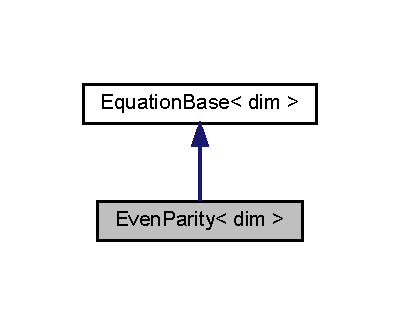
\includegraphics[width=192pt]{class_even_parity__inherit__graph}
\end{center}
\end{figure}


Collaboration diagram for Even\+Parity$<$ dim $>$\+:\nopagebreak
\begin{figure}[H]
\begin{center}
\leavevmode
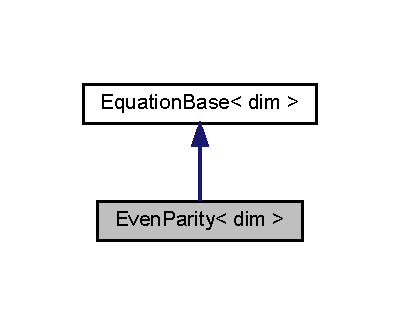
\includegraphics[width=192pt]{class_even_parity__coll__graph}
\end{center}
\end{figure}
\subsection*{Public Member Functions}
\begin{DoxyCompactItemize}
\item 
\hyperlink{class_even_parity_a2877e7e239900be85cc84471fe670abd}{Even\+Parity} (std\+::string \hyperlink{class_equation_base_a0a72472959e531f5256400dec911f3a5}{equation\+\_\+name}, const Parameter\+Handler \&prm, const std\+\_\+cxx11\+::shared\+\_\+ptr$<$ \hyperlink{class_mesh_generator}{Mesh\+Generator}$<$ dim $>$ $>$ msh\+\_\+ptr, const std\+\_\+cxx11\+::shared\+\_\+ptr$<$ \hyperlink{class_a_q_base}{A\+Q\+Base}$<$ dim $>$ $>$ aqd\+\_\+ptr, const std\+\_\+cxx11\+::shared\+\_\+ptr$<$ \hyperlink{class_material_properties}{Material\+Properties} $>$ mat\+\_\+ptr)
\item 
\hyperlink{class_even_parity_a9c3caf641043e0a1e44632478946576b}{$\sim$\+Even\+Parity} ()
\item 
void \hyperlink{class_even_parity_a4cc64002161193e2227e962c9ecb8cf5}{pre\+\_\+assemble\+\_\+cell\+\_\+matrices} (typename Do\+F\+Handler$<$ dim $>$\+::active\+\_\+cell\+\_\+iterator \&cell, std\+::vector$<$ std\+::vector$<$ Full\+Matrix$<$ double $>$ $>$ $>$ \&streaming\+\_\+at\+\_\+qp, std\+::vector$<$ Full\+Matrix$<$ double $>$ $>$ \&collision\+\_\+at\+\_\+qp)
\item 
void \hyperlink{class_even_parity_adb381ea4f45e5ae3741b1d30a0de02b6}{integrate\+\_\+cell\+\_\+bilinear\+\_\+form} (typename Do\+F\+Handler$<$ dim $>$\+::active\+\_\+cell\+\_\+iterator \&cell, Full\+Matrix$<$ double $>$ \&cell\+\_\+matrix, std\+::vector$<$ std\+::vector$<$ Full\+Matrix$<$ double $>$ $>$ $>$ \&streaming\+\_\+at\+\_\+qp, std\+::vector$<$ Full\+Matrix$<$ double $>$ $>$ \&collision\+\_\+at\+\_\+qp, const unsigned int \&g, const unsigned int \&i\+\_\+dir)
\item 
void \hyperlink{class_even_parity_ae800cb49f85cf417167ca5385b50df6f}{integrate\+\_\+boundary\+\_\+bilinear\+\_\+form} (typename Do\+F\+Handler$<$ dim $>$\+::active\+\_\+cell\+\_\+iterator \&cell, unsigned int \&fn, Full\+Matrix$<$ double $>$ \&cell\+\_\+matrix, const unsigned int \&g, const unsigned int \&i\+\_\+dir)
\item 
void \hyperlink{class_even_parity_a0a6674c14f34f22c8ff383aee81ffabf}{integrate\+\_\+interface\+\_\+bilinear\+\_\+form} (typename Do\+F\+Handler$<$ dim $>$\+::active\+\_\+cell\+\_\+iterator \&cell, typename Do\+F\+Handler$<$ dim $>$\+::cell\+\_\+iterator \&neigh, unsigned int \&fn, Full\+Matrix$<$ double $>$ \&vi\+\_\+ui, Full\+Matrix$<$ double $>$ \&vi\+\_\+ue, Full\+Matrix$<$ double $>$ \&ve\+\_\+ui, Full\+Matrix$<$ double $>$ \&ve\+\_\+ue, const unsigned int \&g, const unsigned int \&i\+\_\+dir)
\item 
void \hyperlink{class_even_parity_ad29fd3a026508233ef772ea11f27402e}{integrate\+\_\+scattering\+\_\+linear\+\_\+form} (typename Do\+F\+Handler$<$ dim $>$\+::active\+\_\+cell\+\_\+iterator \&cell, Vector$<$ double $>$ \&cell\+\_\+rhs, std\+::vector$<$ Vector$<$ double $>$ $>$ \&sflxes\+\_\+proc, const unsigned int \&g, const unsigned int \&i\+\_\+dir)
\item 
void \hyperlink{class_even_parity_adc8fad33adf1fae4fb59268b365b21f9}{integrate\+\_\+cell\+\_\+fixed\+\_\+linear\+\_\+form} (typename Do\+F\+Handler$<$ dim $>$\+::active\+\_\+cell\+\_\+iterator \&cell, Vector$<$ double $>$ \&cell\+\_\+rhs, std\+::vector$<$ Vector$<$ double $>$ $>$ \&sflxes\+\_\+prev, const unsigned int \&g, const unsigned int \&i\+\_\+dir)
\end{DoxyCompactItemize}
\subsection*{Private Attributes}
\begin{DoxyCompactItemize}
\item 
double \hyperlink{class_even_parity_a0eeae2ea4837040ebd8df4a997d82acd}{c\+\_\+penalty}
\begin{DoxyCompactList}\small\item\em Polynomial order related part of penalty coefficient. \end{DoxyCompactList}\item 
std\+::vector$<$ double $>$ \hyperlink{class_even_parity_aca63481c4a5de27e6acc2fc72d802303}{tensor\+\_\+norms}
\begin{DoxyCompactList}\small\item\em Frobenius norms of directional tensors (Rank 2). \end{DoxyCompactList}\end{DoxyCompactItemize}
\subsection*{Additional Inherited Members}


\subsection{Detailed Description}
\subsubsection*{template$<$int dim$>$\newline
class Even\+Parity$<$ dim $>$}

This class provides weak formulation for even-\/parity equation. 

The governing equation for this class is the even-\/parity equation. Considering one-\/group steady-\/state equation with isotropic scattering, we transform the angular flux to get a even parity flux\+: \[ \psi^+\left(\vec{\Omega}\right)=\frac{\psi\left(\vec{\Omega}\right)+ \psi\left(-\vec{\Omega}\right)}{2}. \] One would realize\+: \[ \phi=2\int\limits_{2\pi}d\Omega\ \psi^+. \] Skipping all the intermediate steps, one would reach the equation\+: \[ \vec{\Omega}\cdot\nabla\frac{1}{\sigma_\mathrm{t}}\vec{\Omega}\cdot\nabla\psi^+ + \sigma_\mathrm{t}\psi^+= \frac{\sigma_\mathrm{s}}{4\pi}\phi + \frac{\nu\sigma_\mathrm{f}}{4\pi k_\mathrm{eff}}\phi\ (\mathrm{or}\ \frac{Q}{4\pi}). \]

This class implements weak formulation for even-\/parity equation in both D\+F\+EM and C\+F\+EM. D\+F\+EM formulation is based on symmetric interior penalty method combined with formulations specifically for degenerate diffusion equation, which contains a rank 2 tensor in streaming term. Mathematical details of similar formulations are extensively discussed \href{http://epubs.siam.org/doi/abs/1
0.1137/S0036142900374111}{\tt {\bfseries here}}. For details about even-\/parity equation, please refer to \href{http://www.springer.com/cda/cont
ent/document/cda_downloaddocument/9789048134106-c2.pdf?SGWID=0-0-45-1125054-p17
3921104}{\tt {\bfseries E. E. Lewis\textquotesingle{}s book chapter}}.

Related documentation could be found in \href{https://www.dealii.org/8.5.0/
doxygen/deal.II/}{\tt {\bfseries deal.\+II documentation}}.

\begin{DoxyAuthor}{Author}
Weixiong Zheng 
\end{DoxyAuthor}
\begin{DoxyDate}{Date}
2017/05 
\end{DoxyDate}


Definition at line 46 of file even\+\_\+parity.\+h.



\subsection{Constructor \& Destructor Documentation}
\mbox{\Hypertarget{class_even_parity_a2877e7e239900be85cc84471fe670abd}\label{class_even_parity_a2877e7e239900be85cc84471fe670abd}} 
\index{Even\+Parity@{Even\+Parity}!Even\+Parity@{Even\+Parity}}
\index{Even\+Parity@{Even\+Parity}!Even\+Parity@{Even\+Parity}}
\subsubsection{\texorpdfstring{Even\+Parity()}{EvenParity()}}
{\footnotesize\ttfamily template$<$int dim$>$ \\
\hyperlink{class_even_parity}{Even\+Parity}$<$ dim $>$\+::\hyperlink{class_even_parity}{Even\+Parity} (\begin{DoxyParamCaption}\item[{std\+::string}]{equation\+\_\+name,  }\item[{const Parameter\+Handler \&}]{prm,  }\item[{const std\+\_\+cxx11\+::shared\+\_\+ptr$<$ \hyperlink{class_mesh_generator}{Mesh\+Generator}$<$ dim $>$ $>$}]{msh\+\_\+ptr,  }\item[{const std\+\_\+cxx11\+::shared\+\_\+ptr$<$ \hyperlink{class_a_q_base}{A\+Q\+Base}$<$ dim $>$ $>$}]{aqd\+\_\+ptr,  }\item[{const std\+\_\+cxx11\+::shared\+\_\+ptr$<$ \hyperlink{class_material_properties}{Material\+Properties} $>$}]{mat\+\_\+ptr }\end{DoxyParamCaption})}

Class constructor.


\begin{DoxyParams}{Parameters}
{\em equation\+\_\+name} & An abbreviated name of the equation. \\
\hline
{\em msh\+\_\+ptr} & An shared\+\_\+ptr of Mesh\+Generator$<$dim$>$ object. \\
\hline
{\em aqd\+\_\+ptr} & An shared\+\_\+ptr of A\+Q\+Base$<$dim$>$ object. \\
\hline
{\em mat\+\_\+ptr} & An shared\+\_\+ptr of Material\+Properties object. \\
\hline
\end{DoxyParams}


Definition at line 5 of file even\+\_\+parity.\+cc.

\mbox{\Hypertarget{class_even_parity_a9c3caf641043e0a1e44632478946576b}\label{class_even_parity_a9c3caf641043e0a1e44632478946576b}} 
\index{Even\+Parity@{Even\+Parity}!````~Even\+Parity@{$\sim$\+Even\+Parity}}
\index{````~Even\+Parity@{$\sim$\+Even\+Parity}!Even\+Parity@{Even\+Parity}}
\subsubsection{\texorpdfstring{$\sim$\+Even\+Parity()}{~EvenParity()}}
{\footnotesize\ttfamily template$<$int dim$>$ \\
\hyperlink{class_even_parity}{Even\+Parity}$<$ dim $>$\+::$\sim$\hyperlink{class_even_parity}{Even\+Parity} (\begin{DoxyParamCaption}{ }\end{DoxyParamCaption})}

Class destructor. 

Definition at line 29 of file even\+\_\+parity.\+cc.



\subsection{Member Function Documentation}
\mbox{\Hypertarget{class_even_parity_ae800cb49f85cf417167ca5385b50df6f}\label{class_even_parity_ae800cb49f85cf417167ca5385b50df6f}} 
\index{Even\+Parity@{Even\+Parity}!integrate\+\_\+boundary\+\_\+bilinear\+\_\+form@{integrate\+\_\+boundary\+\_\+bilinear\+\_\+form}}
\index{integrate\+\_\+boundary\+\_\+bilinear\+\_\+form@{integrate\+\_\+boundary\+\_\+bilinear\+\_\+form}!Even\+Parity@{Even\+Parity}}
\subsubsection{\texorpdfstring{integrate\+\_\+boundary\+\_\+bilinear\+\_\+form()}{integrate\_boundary\_bilinear\_form()}}
{\footnotesize\ttfamily template$<$int dim$>$ \\
void \hyperlink{class_even_parity}{Even\+Parity}$<$ dim $>$\+::integrate\+\_\+boundary\+\_\+bilinear\+\_\+form (\begin{DoxyParamCaption}\item[{typename Do\+F\+Handler$<$ dim $>$\+::active\+\_\+cell\+\_\+iterator \&}]{cell,  }\item[{unsigned int \&}]{fn,  }\item[{Full\+Matrix$<$ double $>$ \&}]{cell\+\_\+matrix,  }\item[{const unsigned int \&}]{g,  }\item[{const unsigned int \&}]{i\+\_\+dir }\end{DoxyParamCaption})\hspace{0.3cm}{\ttfamily [virtual]}}

This function provides cellwise integrator for bilinear form assembly on boundary.


\begin{DoxyParams}{Parameters}
{\em cell} & Active cell iterator containing cell info. \\
\hline
{\em fn} & Face index in current cell for current boundary face. \\
\hline
{\em cell\+\_\+matrix} & Local cell matrix to be modified in current cell. \\
\hline
{\em g} & Group index. \\
\hline
{\em i\+\_\+dir} & Direction index. \\
\hline
\end{DoxyParams}
\begin{DoxyReturn}{Returns}
Void. 
\end{DoxyReturn}


Reimplemented from \hyperlink{class_equation_base_ae294806284f671619cac9e7169ffff8d}{Equation\+Base$<$ dim $>$}.



Definition at line 78 of file even\+\_\+parity.\+cc.

\mbox{\Hypertarget{class_even_parity_adb381ea4f45e5ae3741b1d30a0de02b6}\label{class_even_parity_adb381ea4f45e5ae3741b1d30a0de02b6}} 
\index{Even\+Parity@{Even\+Parity}!integrate\+\_\+cell\+\_\+bilinear\+\_\+form@{integrate\+\_\+cell\+\_\+bilinear\+\_\+form}}
\index{integrate\+\_\+cell\+\_\+bilinear\+\_\+form@{integrate\+\_\+cell\+\_\+bilinear\+\_\+form}!Even\+Parity@{Even\+Parity}}
\subsubsection{\texorpdfstring{integrate\+\_\+cell\+\_\+bilinear\+\_\+form()}{integrate\_cell\_bilinear\_form()}}
{\footnotesize\ttfamily template$<$int dim$>$ \\
void \hyperlink{class_even_parity}{Even\+Parity}$<$ dim $>$\+::integrate\+\_\+cell\+\_\+bilinear\+\_\+form (\begin{DoxyParamCaption}\item[{typename Do\+F\+Handler$<$ dim $>$\+::active\+\_\+cell\+\_\+iterator \&}]{cell,  }\item[{Full\+Matrix$<$ double $>$ \&}]{cell\+\_\+matrix,  }\item[{std\+::vector$<$ std\+::vector$<$ Full\+Matrix$<$ double $>$ $>$ $>$ \&}]{streaming\+\_\+at\+\_\+qp,  }\item[{std\+::vector$<$ Full\+Matrix$<$ double $>$ $>$ \&}]{collision\+\_\+at\+\_\+qp,  }\item[{const unsigned int \&}]{g,  }\item[{const unsigned int \&}]{i\+\_\+dir }\end{DoxyParamCaption})\hspace{0.3cm}{\ttfamily [virtual]}}

This function provides cell-\/wise integrator for bilinear form. Specifically, this overrides Equation\+Base$<$dim$>$\textquotesingle{}s integrator for even parity equation. Note that interface and boundary face terms are not handled in this integrator.


\begin{DoxyParams}{Parameters}
{\em cell} & Active iterator used to iterating cells. \\
\hline
{\em cell\+\_\+matrix} & Local matrix in bilinear form to be modified. \\
\hline
{\em streaming\+\_\+at\+\_\+qp} & Preassembled streaming matrix per quadrature point. \\
\hline
{\em collision\+\_\+at\+\_\+qp} & Preassembled collision matrix per quadrature point. \\
\hline
{\em g} & Group index. \\
\hline
{\em i\+\_\+dir} & Direction index. \\
\hline
\end{DoxyParams}
\begin{DoxyReturn}{Returns}
Void. 
\end{DoxyReturn}


Reimplemented from \hyperlink{class_equation_base_a7421b3c18433975ac794ac22c3af715a}{Equation\+Base$<$ dim $>$}.



Definition at line 58 of file even\+\_\+parity.\+cc.

\mbox{\Hypertarget{class_even_parity_adc8fad33adf1fae4fb59268b365b21f9}\label{class_even_parity_adc8fad33adf1fae4fb59268b365b21f9}} 
\index{Even\+Parity@{Even\+Parity}!integrate\+\_\+cell\+\_\+fixed\+\_\+linear\+\_\+form@{integrate\+\_\+cell\+\_\+fixed\+\_\+linear\+\_\+form}}
\index{integrate\+\_\+cell\+\_\+fixed\+\_\+linear\+\_\+form@{integrate\+\_\+cell\+\_\+fixed\+\_\+linear\+\_\+form}!Even\+Parity@{Even\+Parity}}
\subsubsection{\texorpdfstring{integrate\+\_\+cell\+\_\+fixed\+\_\+linear\+\_\+form()}{integrate\_cell\_fixed\_linear\_form()}}
{\footnotesize\ttfamily template$<$int dim$>$ \\
void \hyperlink{class_even_parity}{Even\+Parity}$<$ dim $>$\+::integrate\+\_\+cell\+\_\+fixed\+\_\+linear\+\_\+form (\begin{DoxyParamCaption}\item[{typename Do\+F\+Handler$<$ dim $>$\+::active\+\_\+cell\+\_\+iterator \&}]{cell,  }\item[{Vector$<$ double $>$ \&}]{cell\+\_\+rhs,  }\item[{std\+::vector$<$ Vector$<$ double $>$ $>$ \&}]{sflxes\+\_\+prev,  }\item[{const unsigned int \&}]{g,  }\item[{const unsigned int \&}]{i\+\_\+dir }\end{DoxyParamCaption})\hspace{0.3cm}{\ttfamily [virtual]}}

This function provides cellwise integrator for linear form assembly specifically for the contribution of fixed source in fixed-\/source problems or fission in eigenvalue problems.


\begin{DoxyParams}{Parameters}
{\em cell} & Active cell iterator containing cell info. \\
\hline
{\em cell\+\_\+rhs} & Local vector (linear form) to be modified. \\
\hline
{\em sflxes\+\_\+prev} & Scalar fluxes from previous generation due to fission for all groups living on current processor. \\
\hline
{\em g} & Group index. \\
\hline
{\em i\+\_\+dir} & Direction index. \\
\hline
\end{DoxyParams}
\begin{DoxyReturn}{Returns}
Void.
\end{DoxyReturn}
\begin{DoxyNote}{Note}
sflxes\+\_\+prev will do nothing inside the integrator fixed source problems. 
\end{DoxyNote}


Reimplemented from \hyperlink{class_equation_base_ae8472f5c20d76c7d01e5660f8377887e}{Equation\+Base$<$ dim $>$}.



Definition at line 236 of file even\+\_\+parity.\+cc.

\mbox{\Hypertarget{class_even_parity_a0a6674c14f34f22c8ff383aee81ffabf}\label{class_even_parity_a0a6674c14f34f22c8ff383aee81ffabf}} 
\index{Even\+Parity@{Even\+Parity}!integrate\+\_\+interface\+\_\+bilinear\+\_\+form@{integrate\+\_\+interface\+\_\+bilinear\+\_\+form}}
\index{integrate\+\_\+interface\+\_\+bilinear\+\_\+form@{integrate\+\_\+interface\+\_\+bilinear\+\_\+form}!Even\+Parity@{Even\+Parity}}
\subsubsection{\texorpdfstring{integrate\+\_\+interface\+\_\+bilinear\+\_\+form()}{integrate\_interface\_bilinear\_form()}}
{\footnotesize\ttfamily template$<$int dim$>$ \\
void \hyperlink{class_even_parity}{Even\+Parity}$<$ dim $>$\+::integrate\+\_\+interface\+\_\+bilinear\+\_\+form (\begin{DoxyParamCaption}\item[{typename Do\+F\+Handler$<$ dim $>$\+::active\+\_\+cell\+\_\+iterator \&}]{cell,  }\item[{typename Do\+F\+Handler$<$ dim $>$\+::cell\+\_\+iterator \&}]{neigh,  }\item[{unsigned int \&}]{fn,  }\item[{Full\+Matrix$<$ double $>$ \&}]{vi\+\_\+ui,  }\item[{Full\+Matrix$<$ double $>$ \&}]{vi\+\_\+ue,  }\item[{Full\+Matrix$<$ double $>$ \&}]{ve\+\_\+ui,  }\item[{Full\+Matrix$<$ double $>$ \&}]{ve\+\_\+ue,  }\item[{const unsigned int \&}]{g,  }\item[{const unsigned int \&}]{i\+\_\+dir }\end{DoxyParamCaption})\hspace{0.3cm}{\ttfamily [virtual]}}

This function provides integrator for interface bilinear form assembly in D\+F\+EM formulations for even parity using interior penalty method.


\begin{DoxyParams}{Parameters}
{\em cell} & Active cell iterator containing cell info. \\
\hline
{\em neigh} & Cell iterator for neighboring cell about current face. \\
\hline
{\em fn} & Face index in current cell for current boundary face. \\
\hline
{\em vi\+\_\+ui} & Face matrix from testing interior basis by interior basis. \\
\hline
{\em vi\+\_\+ue} & Face matrix from testing exterior basis by interior basis. \\
\hline
{\em ve\+\_\+ui} & Face matrix from testing interior basis by exterior basis. \\
\hline
{\em ve\+\_\+ue} & Face matrix from testing exterior basis by exterior basis. \\
\hline
{\em g} & Group index. \\
\hline
{\em i\+\_\+dir} & Direction index. \\
\hline
\end{DoxyParams}
\begin{DoxyReturn}{Returns}
Void. 
\end{DoxyReturn}


Reimplemented from \hyperlink{class_equation_base_af56caa04c80d8f388e116307930d0063}{Equation\+Base$<$ dim $>$}.



Definition at line 120 of file even\+\_\+parity.\+cc.

\mbox{\Hypertarget{class_even_parity_ad29fd3a026508233ef772ea11f27402e}\label{class_even_parity_ad29fd3a026508233ef772ea11f27402e}} 
\index{Even\+Parity@{Even\+Parity}!integrate\+\_\+scattering\+\_\+linear\+\_\+form@{integrate\+\_\+scattering\+\_\+linear\+\_\+form}}
\index{integrate\+\_\+scattering\+\_\+linear\+\_\+form@{integrate\+\_\+scattering\+\_\+linear\+\_\+form}!Even\+Parity@{Even\+Parity}}
\subsubsection{\texorpdfstring{integrate\+\_\+scattering\+\_\+linear\+\_\+form()}{integrate\_scattering\_linear\_form()}}
{\footnotesize\ttfamily template$<$int dim$>$ \\
void \hyperlink{class_even_parity}{Even\+Parity}$<$ dim $>$\+::integrate\+\_\+scattering\+\_\+linear\+\_\+form (\begin{DoxyParamCaption}\item[{typename Do\+F\+Handler$<$ dim $>$\+::active\+\_\+cell\+\_\+iterator \&}]{cell,  }\item[{Vector$<$ double $>$ \&}]{cell\+\_\+rhs,  }\item[{std\+::vector$<$ Vector$<$ double $>$ $>$ \&}]{sflxes\+\_\+proc,  }\item[{const unsigned int \&}]{g,  }\item[{const unsigned int \&}]{i\+\_\+dir }\end{DoxyParamCaption})\hspace{0.3cm}{\ttfamily [virtual]}}

This function provides cellwise integrator for linear form assembly specifically for the contribution of scattering.


\begin{DoxyParams}{Parameters}
{\em cell} & Active cell iterator containing cell info. \\
\hline
{\em cell\+\_\+rhs} & Local vector (linear form) to be modified. \\
\hline
{\em sflxes\+\_\+proc} & Scalar fluxes for all groups living on current processor. \\
\hline
{\em g} & Group index. \\
\hline
{\em i\+\_\+dir} & Direction index. \\
\hline
\end{DoxyParams}
\begin{DoxyReturn}{Returns}
Void. 
\end{DoxyReturn}


Reimplemented from \hyperlink{class_equation_base_aca5998c1afd2b89ee93d3fbbfde7f3d0}{Equation\+Base$<$ dim $>$}.



Definition at line 209 of file even\+\_\+parity.\+cc.

\mbox{\Hypertarget{class_even_parity_a4cc64002161193e2227e962c9ecb8cf5}\label{class_even_parity_a4cc64002161193e2227e962c9ecb8cf5}} 
\index{Even\+Parity@{Even\+Parity}!pre\+\_\+assemble\+\_\+cell\+\_\+matrices@{pre\+\_\+assemble\+\_\+cell\+\_\+matrices}}
\index{pre\+\_\+assemble\+\_\+cell\+\_\+matrices@{pre\+\_\+assemble\+\_\+cell\+\_\+matrices}!Even\+Parity@{Even\+Parity}}
\subsubsection{\texorpdfstring{pre\+\_\+assemble\+\_\+cell\+\_\+matrices()}{pre\_assemble\_cell\_matrices()}}
{\footnotesize\ttfamily template$<$int dim$>$ \\
void \hyperlink{class_even_parity}{Even\+Parity}$<$ dim $>$\+::pre\+\_\+assemble\+\_\+cell\+\_\+matrices (\begin{DoxyParamCaption}\item[{typename Do\+F\+Handler$<$ dim $>$\+::active\+\_\+cell\+\_\+iterator \&}]{cell,  }\item[{std\+::vector$<$ std\+::vector$<$ Full\+Matrix$<$ double $>$ $>$ $>$ \&}]{streaming\+\_\+at\+\_\+qp,  }\item[{std\+::vector$<$ Full\+Matrix$<$ double $>$ $>$ \&}]{collision\+\_\+at\+\_\+qp }\end{DoxyParamCaption})\hspace{0.3cm}{\ttfamily [virtual]}}

This function provides pre-\/assembled matrices for even-\/parity equation in cell. Current implementation does not include the interface parts, that being said, only C\+F\+EM pre-\/assembly is supported.


\begin{DoxyParams}{Parameters}
{\em cell} & Active iterator used to iterating cells. \\
\hline
{\em streaming\+\_\+at\+\_\+qp} & Vector of streaming matrices per quadrature point. \\
\hline
{\em collision\+\_\+at\+\_\+qp} & Vector of mass matrices per quadrature point. \\
\hline
\end{DoxyParams}
\begin{DoxyReturn}{Returns}
Void. 
\end{DoxyReturn}


Reimplemented from \hyperlink{class_equation_base_a39f0465a523e038302f624f89c08a2ee}{Equation\+Base$<$ dim $>$}.



Definition at line 35 of file even\+\_\+parity.\+cc.



\subsection{Member Data Documentation}
\mbox{\Hypertarget{class_even_parity_a0eeae2ea4837040ebd8df4a997d82acd}\label{class_even_parity_a0eeae2ea4837040ebd8df4a997d82acd}} 
\index{Even\+Parity@{Even\+Parity}!c\+\_\+penalty@{c\+\_\+penalty}}
\index{c\+\_\+penalty@{c\+\_\+penalty}!Even\+Parity@{Even\+Parity}}
\subsubsection{\texorpdfstring{c\+\_\+penalty}{c\_penalty}}
{\footnotesize\ttfamily template$<$int dim$>$ \\
double \hyperlink{class_even_parity}{Even\+Parity}$<$ dim $>$\+::c\+\_\+penalty\hspace{0.3cm}{\ttfamily [private]}}



Polynomial order related part of penalty coefficient. 



Definition at line 190 of file even\+\_\+parity.\+h.

\mbox{\Hypertarget{class_even_parity_aca63481c4a5de27e6acc2fc72d802303}\label{class_even_parity_aca63481c4a5de27e6acc2fc72d802303}} 
\index{Even\+Parity@{Even\+Parity}!tensor\+\_\+norms@{tensor\+\_\+norms}}
\index{tensor\+\_\+norms@{tensor\+\_\+norms}!Even\+Parity@{Even\+Parity}}
\subsubsection{\texorpdfstring{tensor\+\_\+norms}{tensor\_norms}}
{\footnotesize\ttfamily template$<$int dim$>$ \\
std\+::vector$<$double$>$ \hyperlink{class_even_parity}{Even\+Parity}$<$ dim $>$\+::tensor\+\_\+norms\hspace{0.3cm}{\ttfamily [private]}}



Frobenius norms of directional tensors (Rank 2). 

Denoting the directions as column vectors with length of dim, the directional tensor is defined as\+: \[ \mathcal{K}:=\vec{\Omega}\vec{\Omega}^\top, \] which is a Rank 2 tensor as well as a symmetric dimxdim matrix.

For the definition of Fronbenius norm, please refer to \href{http://mathwo
rld.wolfram.com/FrobeniusNorm.html}{\tt {\bfseries wolfram page}}. 

Definition at line 204 of file even\+\_\+parity.\+h.



The documentation for this class was generated from the following files\+:\begin{DoxyCompactItemize}
\item 
src/equation/\hyperlink{even__parity_8h}{even\+\_\+parity.\+h}\item 
src/equation/\hyperlink{even__parity_8cc}{even\+\_\+parity.\+cc}\end{DoxyCompactItemize}

\hypertarget{class_gauss_seidel}{}\section{Gauss\+Seidel$<$ dim $>$ Class Template Reference}
\label{class_gauss_seidel}\index{Gauss\+Seidel$<$ dim $>$@{Gauss\+Seidel$<$ dim $>$}}


This class provides Gauss-\/\+Seidel scheme for MG calculations.  




{\ttfamily \#include $<$gauss\+\_\+seidel.\+h$>$}



Inheritance diagram for Gauss\+Seidel$<$ dim $>$\+:\nopagebreak
\begin{figure}[H]
\begin{center}
\leavevmode
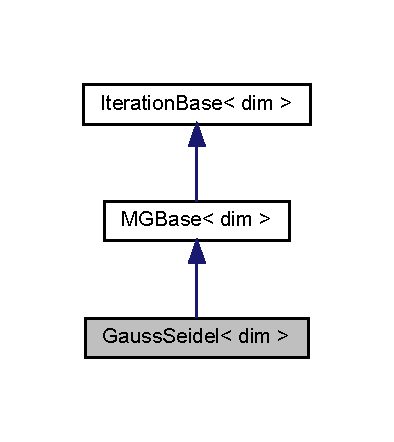
\includegraphics[width=189pt]{class_gauss_seidel__inherit__graph}
\end{center}
\end{figure}


Collaboration diagram for Gauss\+Seidel$<$ dim $>$\+:\nopagebreak
\begin{figure}[H]
\begin{center}
\leavevmode
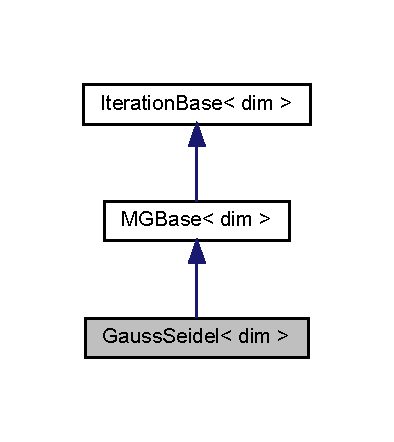
\includegraphics[width=189pt]{class_gauss_seidel__coll__graph}
\end{center}
\end{figure}
\subsection*{Public Member Functions}
\begin{DoxyCompactItemize}
\item 
\hyperlink{class_gauss_seidel_a6024b3a7447aa8fb1cd0bd513c1af81e}{Gauss\+Seidel} (const Parameter\+Handler \&prm)
\item 
\hyperlink{class_gauss_seidel_a4d41231183512ec5aab1fa7088c60788}{$\sim$\+Gauss\+Seidel} ()
\begin{DoxyCompactList}\small\item\em Class destructor. \end{DoxyCompactList}\item 
void \hyperlink{class_gauss_seidel_a28fc4ef9150773f587f90951c704c994}{nonthermal\+\_\+solves} (std\+::vector$<$ Vector$<$ double $>$ $>$ \&sflxes\+\_\+proc, std\+::vector$<$ std\+\_\+cxx11\+::shared\+\_\+ptr$<$ \hyperlink{class_equation_base}{Equation\+Base}$<$ dim $>$ $>$ $>$ \&equ\+\_\+ptrs, std\+\_\+cxx11\+::shared\+\_\+ptr$<$ \hyperlink{class_i_g_base}{I\+G\+Base}$<$ dim $>$ $>$ ig\+\_\+ptr)
\item 
void \hyperlink{class_gauss_seidel_a8db6abbdc88413cbf502ac606b415733}{thermal\+\_\+iterations} (std\+::vector$<$ Vector$<$ double $>$ $>$ \&sflxes\+\_\+proc, std\+::vector$<$ std\+\_\+cxx11\+::shared\+\_\+ptr$<$ \hyperlink{class_equation_base}{Equation\+Base}$<$ dim $>$ $>$ $>$ \&equ\+\_\+ptrs, std\+\_\+cxx11\+::shared\+\_\+ptr$<$ \hyperlink{class_i_g_base}{I\+G\+Base}$<$ dim $>$ $>$ ig\+\_\+ptr)
\end{DoxyCompactItemize}
\subsection*{Additional Inherited Members}


\subsection{Detailed Description}
\subsubsection*{template$<$int dim$>$\newline
class Gauss\+Seidel$<$ dim $>$}

This class provides Gauss-\/\+Seidel scheme for MG calculations. 

This class implements Gauss-\/\+Seidel scheme for MG calculations. Specifically, M\+G\+Base$<$dim$>$\+::nonthermal\+\_\+solves and M\+G\+Base$<$dim$>$\+::thermal\+\_\+iterations are overriden using Gauss-\/\+Seidel iterations.

A Gauss-\/\+Seidel iteration can be represented as\+: \[ T_g\psi_g^{l+1}=\sum\limits_{g'=0}^{g}S_{g'\to g}\psi_{g'}^{l+1}+\sum\limits_{g'=g+1}^{G-1}S_{g'\to g}\psi_{g'}^{l}+Q, \] where $T$, $S$ and $Q$ are transport operator, scattering operator and source and $l$ stands for MG iteration index.

\begin{DoxyAuthor}{Author}
Weixiong Zheng 
\end{DoxyAuthor}
\begin{DoxyDate}{Date}
2017/09 
\end{DoxyDate}


Definition at line 23 of file gauss\+\_\+seidel.\+h.



\subsection{Constructor \& Destructor Documentation}
\mbox{\Hypertarget{class_gauss_seidel_a6024b3a7447aa8fb1cd0bd513c1af81e}\label{class_gauss_seidel_a6024b3a7447aa8fb1cd0bd513c1af81e}} 
\index{Gauss\+Seidel@{Gauss\+Seidel}!Gauss\+Seidel@{Gauss\+Seidel}}
\index{Gauss\+Seidel@{Gauss\+Seidel}!Gauss\+Seidel@{Gauss\+Seidel}}
\subsubsection{\texorpdfstring{Gauss\+Seidel()}{GaussSeidel()}}
{\footnotesize\ttfamily template$<$int dim$>$ \\
\hyperlink{class_gauss_seidel}{Gauss\+Seidel}$<$ dim $>$\+::\hyperlink{class_gauss_seidel}{Gauss\+Seidel} (\begin{DoxyParamCaption}\item[{const Parameter\+Handler \&}]{prm }\end{DoxyParamCaption})}

Class constructor.


\begin{DoxyParams}{Parameters}
{\em prm} & const Parameter\+Handler object. \\
\hline
\end{DoxyParams}


Definition at line 4 of file gauss\+\_\+seidel.\+cc.

\mbox{\Hypertarget{class_gauss_seidel_a4d41231183512ec5aab1fa7088c60788}\label{class_gauss_seidel_a4d41231183512ec5aab1fa7088c60788}} 
\index{Gauss\+Seidel@{Gauss\+Seidel}!````~Gauss\+Seidel@{$\sim$\+Gauss\+Seidel}}
\index{````~Gauss\+Seidel@{$\sim$\+Gauss\+Seidel}!Gauss\+Seidel@{Gauss\+Seidel}}
\subsubsection{\texorpdfstring{$\sim$\+Gauss\+Seidel()}{~GaussSeidel()}}
{\footnotesize\ttfamily template$<$int dim$>$ \\
\hyperlink{class_gauss_seidel}{Gauss\+Seidel}$<$ dim $>$\+::$\sim$\hyperlink{class_gauss_seidel}{Gauss\+Seidel} (\begin{DoxyParamCaption}{ }\end{DoxyParamCaption})}



Class destructor. 



Definition at line 11 of file gauss\+\_\+seidel.\+cc.



\subsection{Member Function Documentation}
\mbox{\Hypertarget{class_gauss_seidel_a28fc4ef9150773f587f90951c704c994}\label{class_gauss_seidel_a28fc4ef9150773f587f90951c704c994}} 
\index{Gauss\+Seidel@{Gauss\+Seidel}!nonthermal\+\_\+solves@{nonthermal\+\_\+solves}}
\index{nonthermal\+\_\+solves@{nonthermal\+\_\+solves}!Gauss\+Seidel@{Gauss\+Seidel}}
\subsubsection{\texorpdfstring{nonthermal\+\_\+solves()}{nonthermal\_solves()}}
{\footnotesize\ttfamily template$<$int dim$>$ \\
void \hyperlink{class_gauss_seidel}{Gauss\+Seidel}$<$ dim $>$\+::nonthermal\+\_\+solves (\begin{DoxyParamCaption}\item[{std\+::vector$<$ Vector$<$ double $>$ $>$ \&}]{sflxes\+\_\+proc,  }\item[{std\+::vector$<$ std\+\_\+cxx11\+::shared\+\_\+ptr$<$ \hyperlink{class_equation_base}{Equation\+Base}$<$ dim $>$ $>$ $>$ \&}]{equ\+\_\+ptrs,  }\item[{std\+\_\+cxx11\+::shared\+\_\+ptr$<$ \hyperlink{class_i_g_base}{I\+G\+Base}$<$ dim $>$ $>$}]{ig\+\_\+ptr }\end{DoxyParamCaption})\hspace{0.3cm}{\ttfamily [virtual]}}

A function overriding M\+G\+Base$<$dim$>$\+::nonthermal\+\_\+solves. The function implements Gauss-\/\+Seidel scheme with one-\/pass serial solves (energy groupwise) from highest energy group until reaching out to the last group before the thermal group boundary.


\begin{DoxyParams}{Parameters}
{\em sflxes\+\_\+proc} & Scalar fluxes living on current processor for all groups. \\
\hline
{\em equ\+\_\+ptrs} & A vector of pointers of Equation\+Base$<$dim$>$ object. \\
\hline
{\em ig\+\_\+ptr} & A pointer of I\+G\+Base$<$dim$>$ object. \\
\hline
\end{DoxyParams}
\begin{DoxyReturn}{Returns}
Void. 
\end{DoxyReturn}


Reimplemented from \hyperlink{class_m_g_base_a55ba9bef3616dd5eab9e3986f6e8e311}{M\+G\+Base$<$ dim $>$}.



Definition at line 17 of file gauss\+\_\+seidel.\+cc.

\mbox{\Hypertarget{class_gauss_seidel_a8db6abbdc88413cbf502ac606b415733}\label{class_gauss_seidel_a8db6abbdc88413cbf502ac606b415733}} 
\index{Gauss\+Seidel@{Gauss\+Seidel}!thermal\+\_\+iterations@{thermal\+\_\+iterations}}
\index{thermal\+\_\+iterations@{thermal\+\_\+iterations}!Gauss\+Seidel@{Gauss\+Seidel}}
\subsubsection{\texorpdfstring{thermal\+\_\+iterations()}{thermal\_iterations()}}
{\footnotesize\ttfamily template$<$int dim$>$ \\
void \hyperlink{class_gauss_seidel}{Gauss\+Seidel}$<$ dim $>$\+::thermal\+\_\+iterations (\begin{DoxyParamCaption}\item[{std\+::vector$<$ Vector$<$ double $>$ $>$ \&}]{sflxes\+\_\+proc,  }\item[{std\+::vector$<$ std\+\_\+cxx11\+::shared\+\_\+ptr$<$ \hyperlink{class_equation_base}{Equation\+Base}$<$ dim $>$ $>$ $>$ \&}]{equ\+\_\+ptrs,  }\item[{std\+\_\+cxx11\+::shared\+\_\+ptr$<$ \hyperlink{class_i_g_base}{I\+G\+Base}$<$ dim $>$ $>$}]{ig\+\_\+ptr }\end{DoxyParamCaption})\hspace{0.3cm}{\ttfamily [virtual]}}

A function overriding M\+G\+Base$<$dim$>$\+::thermal\+\_\+iterations. The function implements Gauss-\/\+Seidel scheme for solving transport problems in thermal groups iteratively. The starting group is the highest energy group affected by upscattering.


\begin{DoxyParams}{Parameters}
{\em sflxes\+\_\+proc} & Scalar fluxes living on current processor for all groups. \\
\hline
{\em equ\+\_\+ptrs} & A vector of pointers of Equation\+Base$<$dim$>$ object. \\
\hline
{\em ig\+\_\+ptr} & A pointer of I\+G\+Base$<$dim$>$ object. \\
\hline
\end{DoxyParams}
\begin{DoxyReturn}{Returns}
Void. 
\end{DoxyReturn}


Reimplemented from \hyperlink{class_m_g_base_a9d3c6ab6e58f0119badb30feedb2ac4d}{M\+G\+Base$<$ dim $>$}.



Definition at line 31 of file gauss\+\_\+seidel.\+cc.



The documentation for this class was generated from the following files\+:\begin{DoxyCompactItemize}
\item 
src/iteration/\hyperlink{gauss__seidel_8h}{gauss\+\_\+seidel.\+h}\item 
src/iteration/\hyperlink{gauss__seidel_8cc}{gauss\+\_\+seidel.\+cc}\end{DoxyCompactItemize}

\hypertarget{class_i_g_base}{}\section{I\+G\+Base$<$ dim $>$ Class Template Reference}
\label{class_i_g_base}\index{I\+G\+Base$<$ dim $>$@{I\+G\+Base$<$ dim $>$}}


This class provides in-\/group solving scheme.  




{\ttfamily \#include $<$ig\+\_\+base.\+h$>$}



Inheritance diagram for I\+G\+Base$<$ dim $>$\+:\nopagebreak
\begin{figure}[H]
\begin{center}
\leavevmode
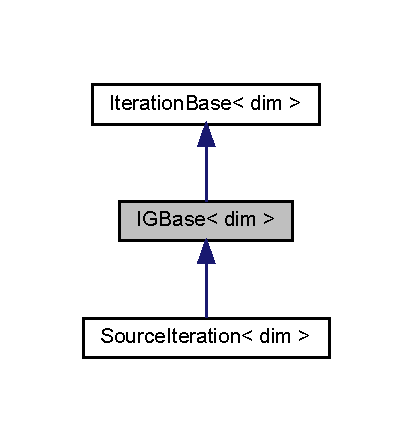
\includegraphics[width=198pt]{class_i_g_base__inherit__graph}
\end{center}
\end{figure}


Collaboration diagram for I\+G\+Base$<$ dim $>$\+:\nopagebreak
\begin{figure}[H]
\begin{center}
\leavevmode
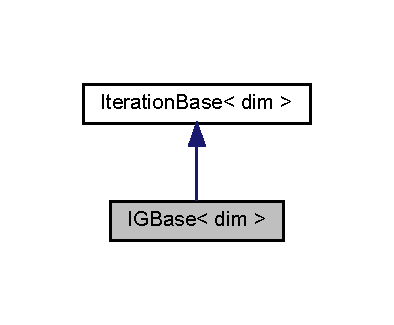
\includegraphics[width=189pt]{class_i_g_base__coll__graph}
\end{center}
\end{figure}
\subsection*{Public Member Functions}
\begin{DoxyCompactItemize}
\item 
\hyperlink{class_i_g_base_a50fb50b4a31894ddf7957f5bed6d74e7}{I\+G\+Base} (const Parameter\+Handler \&prm)
\item 
virtual \hyperlink{class_i_g_base_abde968ae9031dd55de0193896a0134b9}{$\sim$\+I\+G\+Base} ()
\begin{DoxyCompactList}\small\item\em Class destructor. \end{DoxyCompactList}\item 
virtual void \hyperlink{class_i_g_base_a902e919f8b0283be467261f94f79b2c4}{solve\+\_\+in\+\_\+group} (std\+::vector$<$ Vector$<$ double $>$ $>$ \&sflxes\+\_\+proc, std\+\_\+cxx11\+::shared\+\_\+ptr$<$ \hyperlink{class_equation_base}{Equation\+Base}$<$ dim $>$ $>$ equ\+\_\+ptr, unsigned int \&g)
\end{DoxyCompactItemize}
\subsection*{Protected Attributes}
\begin{DoxyCompactItemize}
\item 
const double \hyperlink{class_i_g_base_ace9461aa2cfc9dcc4455616d2d9d6049}{err\+\_\+phi\+\_\+tol}
\begin{DoxyCompactList}\small\item\em Tolerance used in iterative in group scheme for convergence check. \end{DoxyCompactList}\item 
Vector$<$ double $>$ \hyperlink{class_i_g_base_a0a301d6077cb7c94ab0942ab3d5082a5}{sflx\+\_\+proc\+\_\+prev\+\_\+ig}
\end{DoxyCompactItemize}
\subsection*{Additional Inherited Members}


\subsection{Detailed Description}
\subsubsection*{template$<$int dim$>$\newline
class I\+G\+Base$<$ dim $>$}

This class provides in-\/group solving scheme. 

This class serves as the base class for in group solvers. The main (only) functionality is to provide an abstract function for solve in a specific group. Overriding has to be provided in derived class.

\begin{DoxyAuthor}{Author}
Weixiong Zheng 
\end{DoxyAuthor}
\begin{DoxyDate}{Date}
2017/09 
\end{DoxyDate}


Definition at line 18 of file ig\+\_\+base.\+h.



\subsection{Constructor \& Destructor Documentation}
\mbox{\Hypertarget{class_i_g_base_a50fb50b4a31894ddf7957f5bed6d74e7}\label{class_i_g_base_a50fb50b4a31894ddf7957f5bed6d74e7}} 
\index{I\+G\+Base@{I\+G\+Base}!I\+G\+Base@{I\+G\+Base}}
\index{I\+G\+Base@{I\+G\+Base}!I\+G\+Base@{I\+G\+Base}}
\subsubsection{\texorpdfstring{I\+G\+Base()}{IGBase()}}
{\footnotesize\ttfamily template$<$int dim$>$ \\
\hyperlink{class_i_g_base}{I\+G\+Base}$<$ dim $>$\+::\hyperlink{class_i_g_base}{I\+G\+Base} (\begin{DoxyParamCaption}\item[{const Parameter\+Handler \&}]{prm }\end{DoxyParamCaption})}

Class constructor.


\begin{DoxyParams}{Parameters}
{\em prm} & Const Parameter\+Handler object. \\
\hline
\end{DoxyParams}


Definition at line 4 of file ig\+\_\+base.\+cc.

\mbox{\Hypertarget{class_i_g_base_abde968ae9031dd55de0193896a0134b9}\label{class_i_g_base_abde968ae9031dd55de0193896a0134b9}} 
\index{I\+G\+Base@{I\+G\+Base}!````~I\+G\+Base@{$\sim$\+I\+G\+Base}}
\index{````~I\+G\+Base@{$\sim$\+I\+G\+Base}!I\+G\+Base@{I\+G\+Base}}
\subsubsection{\texorpdfstring{$\sim$\+I\+G\+Base()}{~IGBase()}}
{\footnotesize\ttfamily template$<$int dim$>$ \\
\hyperlink{class_i_g_base}{I\+G\+Base}$<$ dim $>$\+::$\sim$\hyperlink{class_i_g_base}{I\+G\+Base} (\begin{DoxyParamCaption}{ }\end{DoxyParamCaption})\hspace{0.3cm}{\ttfamily [virtual]}}



Class destructor. 



Definition at line 12 of file ig\+\_\+base.\+cc.



\subsection{Member Function Documentation}
\mbox{\Hypertarget{class_i_g_base_a902e919f8b0283be467261f94f79b2c4}\label{class_i_g_base_a902e919f8b0283be467261f94f79b2c4}} 
\index{I\+G\+Base@{I\+G\+Base}!solve\+\_\+in\+\_\+group@{solve\+\_\+in\+\_\+group}}
\index{solve\+\_\+in\+\_\+group@{solve\+\_\+in\+\_\+group}!I\+G\+Base@{I\+G\+Base}}
\subsubsection{\texorpdfstring{solve\+\_\+in\+\_\+group()}{solve\_in\_group()}}
{\footnotesize\ttfamily template$<$int dim$>$ \\
void \hyperlink{class_i_g_base}{I\+G\+Base}$<$ dim $>$\+::solve\+\_\+in\+\_\+group (\begin{DoxyParamCaption}\item[{std\+::vector$<$ Vector$<$ double $>$ $>$ \&}]{sflxes\+\_\+proc,  }\item[{std\+\_\+cxx11\+::shared\+\_\+ptr$<$ \hyperlink{class_equation_base}{Equation\+Base}$<$ dim $>$ $>$}]{equ\+\_\+ptr,  }\item[{unsigned int \&}]{g }\end{DoxyParamCaption})\hspace{0.3cm}{\ttfamily [virtual]}}

Abstract function for in group solving functionality. For instance, one could provid overriding as one-\/pass solve for diffusion/\+N\+DA, or iteration based in group solving such as source iteration.


\begin{DoxyParams}{Parameters}
{\em sflxes\+\_\+proc} & A vector of all scalar fluxes on current processor. \\
\hline
{\em equ\+\_\+ptr} & A pointer to the equation of interest. \\
\hline
{\em g} & Group index. \\
\hline
\end{DoxyParams}


Reimplemented in \hyperlink{class_source_iteration_a6d726b9a581391cc4164c29f4ccd1ca5}{Source\+Iteration$<$ dim $>$}.



Definition at line 18 of file ig\+\_\+base.\+cc.



\subsection{Member Data Documentation}
\mbox{\Hypertarget{class_i_g_base_ace9461aa2cfc9dcc4455616d2d9d6049}\label{class_i_g_base_ace9461aa2cfc9dcc4455616d2d9d6049}} 
\index{I\+G\+Base@{I\+G\+Base}!err\+\_\+phi\+\_\+tol@{err\+\_\+phi\+\_\+tol}}
\index{err\+\_\+phi\+\_\+tol@{err\+\_\+phi\+\_\+tol}!I\+G\+Base@{I\+G\+Base}}
\subsubsection{\texorpdfstring{err\+\_\+phi\+\_\+tol}{err\_phi\_tol}}
{\footnotesize\ttfamily template$<$int dim$>$ \\
const double \hyperlink{class_i_g_base}{I\+G\+Base}$<$ dim $>$\+::err\+\_\+phi\+\_\+tol\hspace{0.3cm}{\ttfamily [protected]}}



Tolerance used in iterative in group scheme for convergence check. 



Definition at line 46 of file ig\+\_\+base.\+h.

\mbox{\Hypertarget{class_i_g_base_a0a301d6077cb7c94ab0942ab3d5082a5}\label{class_i_g_base_a0a301d6077cb7c94ab0942ab3d5082a5}} 
\index{I\+G\+Base@{I\+G\+Base}!sflx\+\_\+proc\+\_\+prev\+\_\+ig@{sflx\+\_\+proc\+\_\+prev\+\_\+ig}}
\index{sflx\+\_\+proc\+\_\+prev\+\_\+ig@{sflx\+\_\+proc\+\_\+prev\+\_\+ig}!I\+G\+Base@{I\+G\+Base}}
\subsubsection{\texorpdfstring{sflx\+\_\+proc\+\_\+prev\+\_\+ig}{sflx\_proc\_prev\_ig}}
{\footnotesize\ttfamily template$<$int dim$>$ \\
Vector$<$double$>$ \hyperlink{class_i_g_base}{I\+G\+Base}$<$ dim $>$\+::sflx\+\_\+proc\+\_\+prev\+\_\+ig\hspace{0.3cm}{\ttfamily [protected]}}

Scalar flux value from provious generation.

\begin{DoxyRefDesc}{Todo}
\item[\hyperlink{todo__todo000003}{Todo}]Needs modification if anisotropic scattering is to be implemented. Specifically, a quantities like std\+::vector$<$Vector$<$double$>$ $>$ has to be provided to contain all moments. \end{DoxyRefDesc}


Definition at line 55 of file ig\+\_\+base.\+h.



The documentation for this class was generated from the following files\+:\begin{DoxyCompactItemize}
\item 
src/iteration/\hyperlink{ig__base_8h}{ig\+\_\+base.\+h}\item 
src/iteration/\hyperlink{ig__base_8cc}{ig\+\_\+base.\+cc}\end{DoxyCompactItemize}

\hypertarget{class_iteration_base}{}\section{Iteration\+Base$<$ dim $>$ Class Template Reference}
\label{class_iteration_base}\index{Iteration\+Base$<$ dim $>$@{Iteration\+Base$<$ dim $>$}}


This class provides common functionalities for iteration related classes.  




{\ttfamily \#include $<$iteration\+\_\+base.\+h$>$}



Inheritance diagram for Iteration\+Base$<$ dim $>$\+:\nopagebreak
\begin{figure}[H]
\begin{center}
\leavevmode
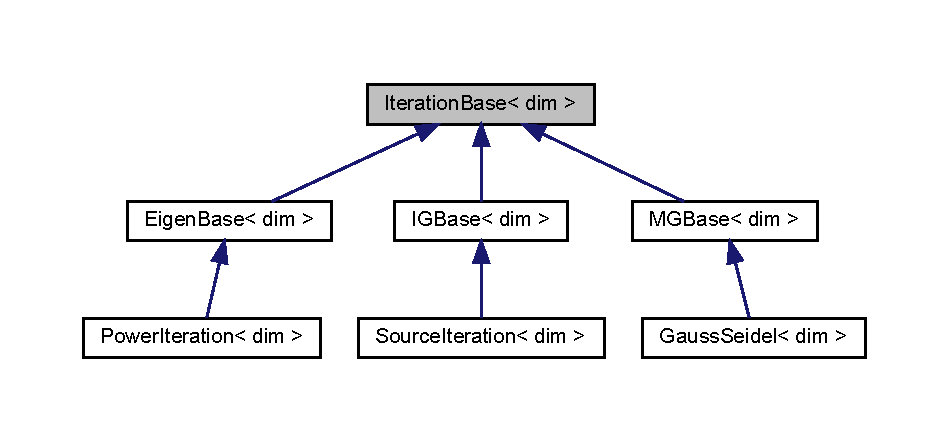
\includegraphics[width=350pt]{class_iteration_base__inherit__graph}
\end{center}
\end{figure}
\subsection*{Public Member Functions}
\begin{DoxyCompactItemize}
\item 
\hyperlink{class_iteration_base_a385009434fcdf512953f317088e09b0b}{Iteration\+Base} (const Parameter\+Handler \&prm)
\item 
virtual \hyperlink{class_iteration_base_a942860f3a03d46da883c1c6c430bea55}{$\sim$\+Iteration\+Base} ()
\begin{DoxyCompactList}\small\item\em Virtual class destructor. \end{DoxyCompactList}\end{DoxyCompactItemize}
\subsection*{Protected Member Functions}
\begin{DoxyCompactItemize}
\item 
double \hyperlink{class_iteration_base_a8bcba214850c5d47f5ae38fb98f51a44}{estimate\+\_\+phi\+\_\+diff} (std\+::vector$<$ P\+E\+T\+Sc\+Wrappers\+::\+M\+P\+I\+::\+Vector $\ast$$>$ \&phis\+\_\+newer, std\+::vector$<$ P\+E\+T\+Sc\+Wrappers\+::\+M\+P\+I\+::\+Vector $\ast$$>$ \&phis\+\_\+older)
\item 
double \hyperlink{class_iteration_base_a5b823c5dda090e64bdba2abb815dfbf6}{estimate\+\_\+phi\+\_\+diff} (P\+E\+T\+Sc\+Wrappers\+::\+M\+P\+I\+::\+Vector $\ast$phi\+\_\+newer, P\+E\+T\+Sc\+Wrappers\+::\+M\+P\+I\+::\+Vector $\ast$phi\+\_\+older)
\item 
double \hyperlink{class_iteration_base_aa929c0e69fd2566db98611b810354123}{estimate\+\_\+phi\+\_\+diff} (std\+::vector$<$ Vector$<$ double $>$ $>$ \&phis\+\_\+newer, std\+::vector$<$ Vector$<$ double $>$ $>$ \&phis\+\_\+older)
\item 
double \hyperlink{class_iteration_base_ab46bde988ac6dc1b84ebb78665414785}{estimate\+\_\+phi\+\_\+diff} (Vector$<$ double $>$ \&phi\+\_\+newer, Vector$<$ double $>$ \&phi\+\_\+older)
\end{DoxyCompactItemize}
\subsection*{Protected Attributes}
\begin{DoxyCompactItemize}
\item 
const unsigned int \hyperlink{class_iteration_base_a0c3ec88894828b2bbe3a5ab4fca927ae}{n\+\_\+group}
\begin{DoxyCompactList}\small\item\em Number of groups. \end{DoxyCompactList}\item 
const bool \hyperlink{class_iteration_base_af630d420379811fe33e19c1c8691ad7c}{is\+\_\+eigen\+\_\+problem}
\begin{DoxyCompactList}\small\item\em Boolean to determine if it\textquotesingle{}s eigenvalue problem. \end{DoxyCompactList}\item 
const bool \hyperlink{class_iteration_base_a871d082ca148eb7976f591f99c2ce81b}{do\+\_\+nda}
\begin{DoxyCompactList}\small\item\em Boolean to determine if N\+DA is used. \end{DoxyCompactList}\item 
double \hyperlink{class_iteration_base_a98cf351c6b85b6bbdc68c914ecdaaf1e}{total\+\_\+calculation\+\_\+time}
\item 
unsigned int \hyperlink{class_iteration_base_afd007145fe5b7bfe22012c44c20d31a4}{ct\+\_\+ho\+\_\+iters}
\item 
unsigned int \hyperlink{class_iteration_base_a1b4bda01b55383e80b0631fbfc339385}{ct\+\_\+nda\+\_\+iters}
\item 
Conditional\+O\+Stream \hyperlink{class_iteration_base_ab057491553962560cfad06f19fb00ff5}{pcout}
\begin{DoxyCompactList}\small\item\em ostream on processor with rank to be 0. \end{DoxyCompactList}\end{DoxyCompactItemize}


\subsection{Detailed Description}
\subsubsection*{template$<$int dim$>$\newline
class Iteration\+Base$<$ dim $>$}

This class provides common functionalities for iteration related classes. 

Currently, it is mainly for providing functionalities on estimating vector differences.

\begin{DoxyAuthor}{Author}
Weixiong 
\end{DoxyAuthor}
\begin{DoxyDate}{Date}
2017/08$\sim$10 
\end{DoxyDate}
\begin{DoxyRefDesc}{Todo}
\item[\hyperlink{todo__todo000004}{Todo}]Implement iteration counting for every type of iteration in calculations. \end{DoxyRefDesc}


Definition at line 20 of file iteration\+\_\+base.\+h.



\subsection{Constructor \& Destructor Documentation}
\mbox{\Hypertarget{class_iteration_base_a385009434fcdf512953f317088e09b0b}\label{class_iteration_base_a385009434fcdf512953f317088e09b0b}} 
\index{Iteration\+Base@{Iteration\+Base}!Iteration\+Base@{Iteration\+Base}}
\index{Iteration\+Base@{Iteration\+Base}!Iteration\+Base@{Iteration\+Base}}
\subsubsection{\texorpdfstring{Iteration\+Base()}{IterationBase()}}
{\footnotesize\ttfamily template$<$int dim$>$ \\
\hyperlink{class_iteration_base}{Iteration\+Base}$<$ dim $>$\+::\hyperlink{class_iteration_base}{Iteration\+Base} (\begin{DoxyParamCaption}\item[{const Parameter\+Handler \&}]{prm }\end{DoxyParamCaption})}

Class constructor.


\begin{DoxyParams}{Parameters}
{\em prm} & Const dealii\+::\+Parameter\+Handler object. \\
\hline
\end{DoxyParams}


Definition at line 4 of file iteration\+\_\+base.\+cc.

\mbox{\Hypertarget{class_iteration_base_a942860f3a03d46da883c1c6c430bea55}\label{class_iteration_base_a942860f3a03d46da883c1c6c430bea55}} 
\index{Iteration\+Base@{Iteration\+Base}!````~Iteration\+Base@{$\sim$\+Iteration\+Base}}
\index{````~Iteration\+Base@{$\sim$\+Iteration\+Base}!Iteration\+Base@{Iteration\+Base}}
\subsubsection{\texorpdfstring{$\sim$\+Iteration\+Base()}{~IterationBase()}}
{\footnotesize\ttfamily template$<$int dim$>$ \\
\hyperlink{class_iteration_base}{Iteration\+Base}$<$ dim $>$\+::$\sim$\hyperlink{class_iteration_base}{Iteration\+Base} (\begin{DoxyParamCaption}{ }\end{DoxyParamCaption})\hspace{0.3cm}{\ttfamily [virtual]}}



Virtual class destructor. 



Definition at line 15 of file iteration\+\_\+base.\+cc.



\subsection{Member Function Documentation}
\mbox{\Hypertarget{class_iteration_base_a8bcba214850c5d47f5ae38fb98f51a44}\label{class_iteration_base_a8bcba214850c5d47f5ae38fb98f51a44}} 
\index{Iteration\+Base@{Iteration\+Base}!estimate\+\_\+phi\+\_\+diff@{estimate\+\_\+phi\+\_\+diff}}
\index{estimate\+\_\+phi\+\_\+diff@{estimate\+\_\+phi\+\_\+diff}!Iteration\+Base@{Iteration\+Base}}
\subsubsection{\texorpdfstring{estimate\+\_\+phi\+\_\+diff()}{estimate\_phi\_diff()}\hspace{0.1cm}{\footnotesize\ttfamily [1/4]}}
{\footnotesize\ttfamily template$<$int dim$>$ \\
double \hyperlink{class_iteration_base}{Iteration\+Base}$<$ dim $>$\+::estimate\+\_\+phi\+\_\+diff (\begin{DoxyParamCaption}\item[{std\+::vector$<$ P\+E\+T\+Sc\+Wrappers\+::\+M\+P\+I\+::\+Vector $\ast$$>$ \&}]{phis\+\_\+newer,  }\item[{std\+::vector$<$ P\+E\+T\+Sc\+Wrappers\+::\+M\+P\+I\+::\+Vector $\ast$$>$ \&}]{phis\+\_\+older }\end{DoxyParamCaption})\hspace{0.3cm}{\ttfamily [protected]}}

Function to measure the relative difference between two sets of P\+E\+T\+Sc Vectors


\begin{DoxyParams}{Parameters}
{\em Two} & sets of P\+E\+T\+Sc Vectors with the same length \\
\hline
\end{DoxyParams}
\begin{DoxyReturn}{Returns}
relative difference in vector l1 norm measure 
\end{DoxyReturn}


Definition at line 26 of file iteration\+\_\+base.\+cc.

\mbox{\Hypertarget{class_iteration_base_a5b823c5dda090e64bdba2abb815dfbf6}\label{class_iteration_base_a5b823c5dda090e64bdba2abb815dfbf6}} 
\index{Iteration\+Base@{Iteration\+Base}!estimate\+\_\+phi\+\_\+diff@{estimate\+\_\+phi\+\_\+diff}}
\index{estimate\+\_\+phi\+\_\+diff@{estimate\+\_\+phi\+\_\+diff}!Iteration\+Base@{Iteration\+Base}}
\subsubsection{\texorpdfstring{estimate\+\_\+phi\+\_\+diff()}{estimate\_phi\_diff()}\hspace{0.1cm}{\footnotesize\ttfamily [2/4]}}
{\footnotesize\ttfamily template$<$int dim$>$ \\
double \hyperlink{class_iteration_base}{Iteration\+Base}$<$ dim $>$\+::estimate\+\_\+phi\+\_\+diff (\begin{DoxyParamCaption}\item[{P\+E\+T\+Sc\+Wrappers\+::\+M\+P\+I\+::\+Vector $\ast$}]{phi\+\_\+newer,  }\item[{P\+E\+T\+Sc\+Wrappers\+::\+M\+P\+I\+::\+Vector $\ast$}]{phi\+\_\+older }\end{DoxyParamCaption})\hspace{0.3cm}{\ttfamily [protected]}}

Function to measure the relative difference between two P\+E\+T\+Sc Vectors


\begin{DoxyParams}{Parameters}
{\em Two} & P\+E\+T\+Sc Vectors with the same length \\
\hline
\end{DoxyParams}
\begin{DoxyReturn}{Returns}
relative difference in vector l1 norm measure 
\end{DoxyReturn}


Definition at line 43 of file iteration\+\_\+base.\+cc.

\mbox{\Hypertarget{class_iteration_base_aa929c0e69fd2566db98611b810354123}\label{class_iteration_base_aa929c0e69fd2566db98611b810354123}} 
\index{Iteration\+Base@{Iteration\+Base}!estimate\+\_\+phi\+\_\+diff@{estimate\+\_\+phi\+\_\+diff}}
\index{estimate\+\_\+phi\+\_\+diff@{estimate\+\_\+phi\+\_\+diff}!Iteration\+Base@{Iteration\+Base}}
\subsubsection{\texorpdfstring{estimate\+\_\+phi\+\_\+diff()}{estimate\_phi\_diff()}\hspace{0.1cm}{\footnotesize\ttfamily [3/4]}}
{\footnotesize\ttfamily template$<$int dim$>$ \\
double \hyperlink{class_iteration_base}{Iteration\+Base}$<$ dim $>$\+::estimate\+\_\+phi\+\_\+diff (\begin{DoxyParamCaption}\item[{std\+::vector$<$ Vector$<$ double $>$ $>$ \&}]{phis\+\_\+newer,  }\item[{std\+::vector$<$ Vector$<$ double $>$ $>$ \&}]{phis\+\_\+older }\end{DoxyParamCaption})\hspace{0.3cm}{\ttfamily [protected]}}

Function to measure the relative difference between two P\+E\+T\+Sc M\+PI Vectors.


\begin{DoxyParams}{Parameters}
{\em Two} & sets of P\+E\+T\+Sc Vectors with the same length \\
\hline
\end{DoxyParams}
\begin{DoxyReturn}{Returns}
relative difference in vector l1 norm measure 
\end{DoxyReturn}


Definition at line 53 of file iteration\+\_\+base.\+cc.

\mbox{\Hypertarget{class_iteration_base_ab46bde988ac6dc1b84ebb78665414785}\label{class_iteration_base_ab46bde988ac6dc1b84ebb78665414785}} 
\index{Iteration\+Base@{Iteration\+Base}!estimate\+\_\+phi\+\_\+diff@{estimate\+\_\+phi\+\_\+diff}}
\index{estimate\+\_\+phi\+\_\+diff@{estimate\+\_\+phi\+\_\+diff}!Iteration\+Base@{Iteration\+Base}}
\subsubsection{\texorpdfstring{estimate\+\_\+phi\+\_\+diff()}{estimate\_phi\_diff()}\hspace{0.1cm}{\footnotesize\ttfamily [4/4]}}
{\footnotesize\ttfamily template$<$int dim$>$ \\
double \hyperlink{class_iteration_base}{Iteration\+Base}$<$ dim $>$\+::estimate\+\_\+phi\+\_\+diff (\begin{DoxyParamCaption}\item[{Vector$<$ double $>$ \&}]{phi\+\_\+newer,  }\item[{Vector$<$ double $>$ \&}]{phi\+\_\+older }\end{DoxyParamCaption})\hspace{0.3cm}{\ttfamily [protected]}}

Function to measure the relative difference between two sets of deal.\+II Vectors. Note that though all vectors live on current processor, broadcast is performed to obtain global results.


\begin{DoxyParams}{Parameters}
{\em Two} & deal.\+II Vectors with the same length \\
\hline
\end{DoxyParams}
\begin{DoxyReturn}{Returns}
relative difference in vector l1 norm measure 
\end{DoxyReturn}


Definition at line 74 of file iteration\+\_\+base.\+cc.



\subsection{Member Data Documentation}
\mbox{\Hypertarget{class_iteration_base_afd007145fe5b7bfe22012c44c20d31a4}\label{class_iteration_base_afd007145fe5b7bfe22012c44c20d31a4}} 
\index{Iteration\+Base@{Iteration\+Base}!ct\+\_\+ho\+\_\+iters@{ct\+\_\+ho\+\_\+iters}}
\index{ct\+\_\+ho\+\_\+iters@{ct\+\_\+ho\+\_\+iters}!Iteration\+Base@{Iteration\+Base}}
\subsubsection{\texorpdfstring{ct\+\_\+ho\+\_\+iters}{ct\_ho\_iters}}
{\footnotesize\ttfamily template$<$int dim$>$ \\
unsigned int \hyperlink{class_iteration_base}{Iteration\+Base}$<$ dim $>$\+::ct\+\_\+ho\+\_\+iters\hspace{0.3cm}{\ttfamily [protected]}}

HO iteration counts 

Definition at line 81 of file iteration\+\_\+base.\+h.

\mbox{\Hypertarget{class_iteration_base_a1b4bda01b55383e80b0631fbfc339385}\label{class_iteration_base_a1b4bda01b55383e80b0631fbfc339385}} 
\index{Iteration\+Base@{Iteration\+Base}!ct\+\_\+nda\+\_\+iters@{ct\+\_\+nda\+\_\+iters}}
\index{ct\+\_\+nda\+\_\+iters@{ct\+\_\+nda\+\_\+iters}!Iteration\+Base@{Iteration\+Base}}
\subsubsection{\texorpdfstring{ct\+\_\+nda\+\_\+iters}{ct\_nda\_iters}}
{\footnotesize\ttfamily template$<$int dim$>$ \\
unsigned int \hyperlink{class_iteration_base}{Iteration\+Base}$<$ dim $>$\+::ct\+\_\+nda\+\_\+iters\hspace{0.3cm}{\ttfamily [protected]}}

N\+DA iteration counts 

Definition at line 82 of file iteration\+\_\+base.\+h.

\mbox{\Hypertarget{class_iteration_base_a871d082ca148eb7976f591f99c2ce81b}\label{class_iteration_base_a871d082ca148eb7976f591f99c2ce81b}} 
\index{Iteration\+Base@{Iteration\+Base}!do\+\_\+nda@{do\+\_\+nda}}
\index{do\+\_\+nda@{do\+\_\+nda}!Iteration\+Base@{Iteration\+Base}}
\subsubsection{\texorpdfstring{do\+\_\+nda}{do\_nda}}
{\footnotesize\ttfamily template$<$int dim$>$ \\
const bool \hyperlink{class_iteration_base}{Iteration\+Base}$<$ dim $>$\+::do\+\_\+nda\hspace{0.3cm}{\ttfamily [protected]}}



Boolean to determine if N\+DA is used. 



Definition at line 78 of file iteration\+\_\+base.\+h.

\mbox{\Hypertarget{class_iteration_base_af630d420379811fe33e19c1c8691ad7c}\label{class_iteration_base_af630d420379811fe33e19c1c8691ad7c}} 
\index{Iteration\+Base@{Iteration\+Base}!is\+\_\+eigen\+\_\+problem@{is\+\_\+eigen\+\_\+problem}}
\index{is\+\_\+eigen\+\_\+problem@{is\+\_\+eigen\+\_\+problem}!Iteration\+Base@{Iteration\+Base}}
\subsubsection{\texorpdfstring{is\+\_\+eigen\+\_\+problem}{is\_eigen\_problem}}
{\footnotesize\ttfamily template$<$int dim$>$ \\
const bool \hyperlink{class_iteration_base}{Iteration\+Base}$<$ dim $>$\+::is\+\_\+eigen\+\_\+problem\hspace{0.3cm}{\ttfamily [protected]}}



Boolean to determine if it\textquotesingle{}s eigenvalue problem. 



Definition at line 77 of file iteration\+\_\+base.\+h.

\mbox{\Hypertarget{class_iteration_base_a0c3ec88894828b2bbe3a5ab4fca927ae}\label{class_iteration_base_a0c3ec88894828b2bbe3a5ab4fca927ae}} 
\index{Iteration\+Base@{Iteration\+Base}!n\+\_\+group@{n\+\_\+group}}
\index{n\+\_\+group@{n\+\_\+group}!Iteration\+Base@{Iteration\+Base}}
\subsubsection{\texorpdfstring{n\+\_\+group}{n\_group}}
{\footnotesize\ttfamily template$<$int dim$>$ \\
const unsigned int \hyperlink{class_iteration_base}{Iteration\+Base}$<$ dim $>$\+::n\+\_\+group\hspace{0.3cm}{\ttfamily [protected]}}



Number of groups. 



Definition at line 76 of file iteration\+\_\+base.\+h.

\mbox{\Hypertarget{class_iteration_base_ab057491553962560cfad06f19fb00ff5}\label{class_iteration_base_ab057491553962560cfad06f19fb00ff5}} 
\index{Iteration\+Base@{Iteration\+Base}!pcout@{pcout}}
\index{pcout@{pcout}!Iteration\+Base@{Iteration\+Base}}
\subsubsection{\texorpdfstring{pcout}{pcout}}
{\footnotesize\ttfamily template$<$int dim$>$ \\
Conditional\+O\+Stream \hyperlink{class_iteration_base}{Iteration\+Base}$<$ dim $>$\+::pcout\hspace{0.3cm}{\ttfamily [protected]}}



ostream on processor with rank to be 0. 

Details can be found \href{https://www.dealii.org/8.5.0/doxygen/deal.II/cl
assConditionalOStream.html}{\tt {\bfseries here}}. 

Definition at line 89 of file iteration\+\_\+base.\+h.

\mbox{\Hypertarget{class_iteration_base_a98cf351c6b85b6bbdc68c914ecdaaf1e}\label{class_iteration_base_a98cf351c6b85b6bbdc68c914ecdaaf1e}} 
\index{Iteration\+Base@{Iteration\+Base}!total\+\_\+calculation\+\_\+time@{total\+\_\+calculation\+\_\+time}}
\index{total\+\_\+calculation\+\_\+time@{total\+\_\+calculation\+\_\+time}!Iteration\+Base@{Iteration\+Base}}
\subsubsection{\texorpdfstring{total\+\_\+calculation\+\_\+time}{total\_calculation\_time}}
{\footnotesize\ttfamily template$<$int dim$>$ \\
double \hyperlink{class_iteration_base}{Iteration\+Base}$<$ dim $>$\+::total\+\_\+calculation\+\_\+time\hspace{0.3cm}{\ttfamily [protected]}}

total time for calculations+assemblies 

Definition at line 80 of file iteration\+\_\+base.\+h.



The documentation for this class was generated from the following files\+:\begin{DoxyCompactItemize}
\item 
src/iteration/\hyperlink{iteration__base_8h}{iteration\+\_\+base.\+h}\item 
src/iteration/\hyperlink{iteration__base_8cc}{iteration\+\_\+base.\+cc}\end{DoxyCompactItemize}

\hypertarget{class_iterations}{}\section{Iterations$<$ dim $>$ Class Template Reference}
\label{class_iterations}\index{Iterations$<$ dim $>$@{Iterations$<$ dim $>$}}


This class provide an interface between Bart\+Driver and specific iteration schemes.  




{\ttfamily \#include $<$iterations.\+h$>$}

\subsection*{Public Member Functions}
\begin{DoxyCompactItemize}
\item 
\hyperlink{class_iterations_a0355678383cd174840beb772ce7e9e8d}{Iterations} (const Parameter\+Handler \&prm)
\item 
\hyperlink{class_iterations_ae6ea082615afe8919000b4ea1465f9cf}{$\sim$\+Iterations} ()
\begin{DoxyCompactList}\small\item\em Class destructor. \end{DoxyCompactList}\item 
void \hyperlink{class_iterations_ae41347e35b05b6f0fd3cb2a03ab60341}{solve\+\_\+problems} (std\+::vector$<$ Vector$<$ double $>$ $>$ \&sflxes\+\_\+proc, std\+::vector$<$ std\+\_\+cxx11\+::shared\+\_\+ptr$<$ \hyperlink{class_equation_base}{Equation\+Base}$<$ dim $>$ $>$ $>$ \&equ\+\_\+ptrs, std\+\_\+cxx11\+::shared\+\_\+ptr$<$ \hyperlink{class_i_g_base}{I\+G\+Base}$<$ dim $>$ $>$ ig\+\_\+ptr, std\+\_\+cxx11\+::shared\+\_\+ptr$<$ \hyperlink{class_m_g_base}{M\+G\+Base}$<$ dim $>$ $>$ mg\+\_\+ptr, std\+\_\+cxx11\+::shared\+\_\+ptr$<$ \hyperlink{class_eigen_base}{Eigen\+Base}$<$ dim $>$ $>$ eig\+\_\+ptr)
\end{DoxyCompactItemize}
\subsection*{Private Attributes}
\begin{DoxyCompactItemize}
\item 
const std\+::string \hyperlink{class_iterations_a3a29339b09351ffa95e9c99be5d5e575}{transport\+\_\+name}
\begin{DoxyCompactList}\small\item\em HO equation name. \end{DoxyCompactList}\item 
double \hyperlink{class_iterations_a4c36c8bdd6775be8015ef113c68a1e66}{keff}
\begin{DoxyCompactList}\small\item\em keff living in current class. \end{DoxyCompactList}\item 
bool \hyperlink{class_iterations_acfd49ecddab96b70fc271942b3173ad7}{is\+\_\+eigen\+\_\+problem}
\begin{DoxyCompactList}\small\item\em Boolean to determine if the problem is eigenvalue problem. \end{DoxyCompactList}\end{DoxyCompactItemize}


\subsection{Detailed Description}
\subsubsection*{template$<$int dim$>$\newline
class Iterations$<$ dim $>$}

This class provide an interface between Bart\+Driver and specific iteration schemes. 

This class implements an interface between Bart\+Driver$<$dim$>$ and iteration schemes. The main purpose is such that one would not need to develop different functions according to different problem types. 

Definition at line 23 of file iterations.\+h.



\subsection{Constructor \& Destructor Documentation}
\mbox{\Hypertarget{class_iterations_a0355678383cd174840beb772ce7e9e8d}\label{class_iterations_a0355678383cd174840beb772ce7e9e8d}} 
\index{Iterations@{Iterations}!Iterations@{Iterations}}
\index{Iterations@{Iterations}!Iterations@{Iterations}}
\subsubsection{\texorpdfstring{Iterations()}{Iterations()}}
{\footnotesize\ttfamily template$<$int dim$>$ \\
\hyperlink{class_iterations}{Iterations}$<$ dim $>$\+::\hyperlink{class_iterations}{Iterations} (\begin{DoxyParamCaption}\item[{const Parameter\+Handler \&}]{prm }\end{DoxyParamCaption})}

Class constructor.


\begin{DoxyParams}{Parameters}
{\em prm} & const Parameter\+Handler object. \\
\hline
\end{DoxyParams}


Definition at line 7 of file iterations.\+cc.

\mbox{\Hypertarget{class_iterations_ae6ea082615afe8919000b4ea1465f9cf}\label{class_iterations_ae6ea082615afe8919000b4ea1465f9cf}} 
\index{Iterations@{Iterations}!````~Iterations@{$\sim$\+Iterations}}
\index{````~Iterations@{$\sim$\+Iterations}!Iterations@{Iterations}}
\subsubsection{\texorpdfstring{$\sim$\+Iterations()}{~Iterations()}}
{\footnotesize\ttfamily template$<$int dim$>$ \\
\hyperlink{class_iterations}{Iterations}$<$ dim $>$\+::$\sim$\hyperlink{class_iterations}{Iterations} (\begin{DoxyParamCaption}{ }\end{DoxyParamCaption})}



Class destructor. 



Definition at line 15 of file iterations.\+cc.



\subsection{Member Function Documentation}
\mbox{\Hypertarget{class_iterations_ae41347e35b05b6f0fd3cb2a03ab60341}\label{class_iterations_ae41347e35b05b6f0fd3cb2a03ab60341}} 
\index{Iterations@{Iterations}!solve\+\_\+problems@{solve\+\_\+problems}}
\index{solve\+\_\+problems@{solve\+\_\+problems}!Iterations@{Iterations}}
\subsubsection{\texorpdfstring{solve\+\_\+problems()}{solve\_problems()}}
{\footnotesize\ttfamily template$<$int dim$>$ \\
void \hyperlink{class_iterations}{Iterations}$<$ dim $>$\+::solve\+\_\+problems (\begin{DoxyParamCaption}\item[{std\+::vector$<$ Vector$<$ double $>$ $>$ \&}]{sflxes\+\_\+proc,  }\item[{std\+::vector$<$ std\+\_\+cxx11\+::shared\+\_\+ptr$<$ \hyperlink{class_equation_base}{Equation\+Base}$<$ dim $>$ $>$ $>$ \&}]{equ\+\_\+ptrs,  }\item[{std\+\_\+cxx11\+::shared\+\_\+ptr$<$ \hyperlink{class_i_g_base}{I\+G\+Base}$<$ dim $>$ $>$}]{ig\+\_\+ptr,  }\item[{std\+\_\+cxx11\+::shared\+\_\+ptr$<$ \hyperlink{class_m_g_base}{M\+G\+Base}$<$ dim $>$ $>$}]{mg\+\_\+ptr,  }\item[{std\+\_\+cxx11\+::shared\+\_\+ptr$<$ \hyperlink{class_eigen_base}{Eigen\+Base}$<$ dim $>$ $>$}]{eig\+\_\+ptr }\end{DoxyParamCaption})}

A generic function to solve the problem for both eigenvalue and fixed-\/source problems. Inside this function, solving methods will be specified according to Iterations$<$dim$>$\+::is\+\_\+eigen\+\_\+problem the boolean.

\begin{DoxyNote}{Note}
In fixed-\/source problems, eig\+\_\+ptr points to a null pointer and will do nothing.
\end{DoxyNote}

\begin{DoxyParams}{Parameters}
{\em equ\+\_\+ptrs} & A vector of shared\+\_\+ptr\textquotesingle{}s of Equation\+Base objects. \\
\hline
{\em ig\+\_\+ptr} & A shared\+\_\+ptr of downcast I\+G\+Base object. \\
\hline
{\em mg\+\_\+ptr} & A shared\+\_\+ptr of downcast M\+G\+Base object. \\
\hline
{\em eig\+\_\+ptr} & A shared\+\_\+ptr of downcast Eigen\+Base object. \\
\hline
\end{DoxyParams}
\begin{DoxyReturn}{Returns}
Void. 
\end{DoxyReturn}


Definition at line 21 of file iterations.\+cc.



\subsection{Member Data Documentation}
\mbox{\Hypertarget{class_iterations_acfd49ecddab96b70fc271942b3173ad7}\label{class_iterations_acfd49ecddab96b70fc271942b3173ad7}} 
\index{Iterations@{Iterations}!is\+\_\+eigen\+\_\+problem@{is\+\_\+eigen\+\_\+problem}}
\index{is\+\_\+eigen\+\_\+problem@{is\+\_\+eigen\+\_\+problem}!Iterations@{Iterations}}
\subsubsection{\texorpdfstring{is\+\_\+eigen\+\_\+problem}{is\_eigen\_problem}}
{\footnotesize\ttfamily template$<$int dim$>$ \\
bool \hyperlink{class_iterations}{Iterations}$<$ dim $>$\+::is\+\_\+eigen\+\_\+problem\hspace{0.3cm}{\ttfamily [private]}}



Boolean to determine if the problem is eigenvalue problem. 



Definition at line 61 of file iterations.\+h.

\mbox{\Hypertarget{class_iterations_a4c36c8bdd6775be8015ef113c68a1e66}\label{class_iterations_a4c36c8bdd6775be8015ef113c68a1e66}} 
\index{Iterations@{Iterations}!keff@{keff}}
\index{keff@{keff}!Iterations@{Iterations}}
\subsubsection{\texorpdfstring{keff}{keff}}
{\footnotesize\ttfamily template$<$int dim$>$ \\
double \hyperlink{class_iterations}{Iterations}$<$ dim $>$\+::keff\hspace{0.3cm}{\ttfamily [private]}}



keff living in current class. 



Definition at line 60 of file iterations.\+h.

\mbox{\Hypertarget{class_iterations_a3a29339b09351ffa95e9c99be5d5e575}\label{class_iterations_a3a29339b09351ffa95e9c99be5d5e575}} 
\index{Iterations@{Iterations}!transport\+\_\+name@{transport\+\_\+name}}
\index{transport\+\_\+name@{transport\+\_\+name}!Iterations@{Iterations}}
\subsubsection{\texorpdfstring{transport\+\_\+name}{transport\_name}}
{\footnotesize\ttfamily template$<$int dim$>$ \\
const std\+::string \hyperlink{class_iterations}{Iterations}$<$ dim $>$\+::transport\+\_\+name\hspace{0.3cm}{\ttfamily [private]}}



HO equation name. 



Definition at line 58 of file iterations.\+h.



The documentation for this class was generated from the following files\+:\begin{DoxyCompactItemize}
\item 
src/iteration/\hyperlink{iterations_8h}{iterations.\+h}\item 
src/iteration/\hyperlink{iterations_8cc}{iterations.\+cc}\end{DoxyCompactItemize}

\hypertarget{class_l_s_g_c}{}\section{L\+S\+GC$<$ dim $>$ Class Template Reference}
\label{class_l_s_g_c}\index{L\+S\+G\+C$<$ dim $>$@{L\+S\+G\+C$<$ dim $>$}}


This class produces level-\/symmetric Gauss-\/\+Chebyshev quadrature.  




{\ttfamily \#include $<$lsgc.\+h$>$}



Inheritance diagram for L\+S\+GC$<$ dim $>$\+:\nopagebreak
\begin{figure}[H]
\begin{center}
\leavevmode
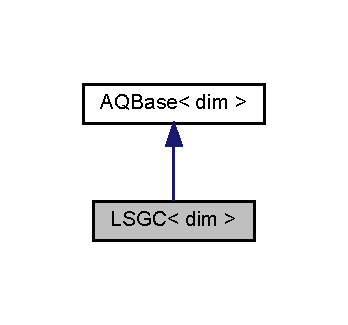
\includegraphics[width=167pt]{class_l_s_g_c__inherit__graph}
\end{center}
\end{figure}


Collaboration diagram for L\+S\+GC$<$ dim $>$\+:\nopagebreak
\begin{figure}[H]
\begin{center}
\leavevmode
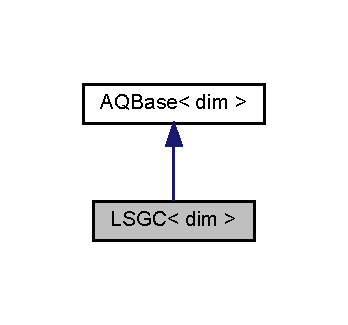
\includegraphics[width=167pt]{class_l_s_g_c__coll__graph}
\end{center}
\end{figure}
\subsection*{Public Member Functions}
\begin{DoxyCompactItemize}
\item 
\hyperlink{class_l_s_g_c_a9b89f615563bd3583a4a6a36d7b3eb7d}{L\+S\+GC} (Parameter\+Handler \&prm)
\begin{DoxyCompactList}\small\item\em Destructor. \end{DoxyCompactList}\item 
\hyperlink{class_l_s_g_c_abcba8afdb075485278288db321776b7e}{$\sim$\+L\+S\+GC} ()
\item 
void \hyperlink{class_l_s_g_c_a1d135fb9ca12a9b65b8cc397479fc4d7}{produce\+\_\+angular\+\_\+quad} ()
\end{DoxyCompactItemize}
\subsection*{Additional Inherited Members}


\subsection{Detailed Description}
\subsubsection*{template$<$int dim$>$\newline
class L\+S\+G\+C$<$ dim $>$}

This class produces level-\/symmetric Gauss-\/\+Chebyshev quadrature. 

This class is derived from A\+Q\+Base$<$dim$>$ with L\+S\+GC rule. The polar angular points are determined by 1D Gauss-\/\+Legendre quadrature. Azimuthally, the points are placed uniformly per polar level. Detailed descriptions can be found in literature such as \href{http://oaktrust.library.tamu.edu/bitstream/handle/1969.1/ETD-T
AMU-2010-12-8586/JARRELL-DISSERTATION.pdf?sequence=2}{\tt {\bfseries  J. J. Jarrell\textquotesingle{}s dissertation}}.

\begin{DoxyAuthor}{Author}
Weixiong Zheng 
\end{DoxyAuthor}
\begin{DoxyDate}{Date}
2017/04 
\end{DoxyDate}


Definition at line 21 of file lsgc.\+h.



\subsection{Constructor \& Destructor Documentation}
\mbox{\Hypertarget{class_l_s_g_c_a9b89f615563bd3583a4a6a36d7b3eb7d}\label{class_l_s_g_c_a9b89f615563bd3583a4a6a36d7b3eb7d}} 
\index{L\+S\+GC@{L\+S\+GC}!L\+S\+GC@{L\+S\+GC}}
\index{L\+S\+GC@{L\+S\+GC}!L\+S\+GC@{L\+S\+GC}}
\subsubsection{\texorpdfstring{L\+S\+G\+C()}{LSGC()}}
{\footnotesize\ttfamily template$<$int dim$>$ \\
\hyperlink{class_l_s_g_c}{L\+S\+GC}$<$ dim $>$\+::\hyperlink{class_l_s_g_c}{L\+S\+GC} (\begin{DoxyParamCaption}\item[{Parameter\+Handler \&}]{prm }\end{DoxyParamCaption})}



Destructor. 

Class constructor.


\begin{DoxyParams}{Parameters}
{\em prm} & Parameter\+Handler object. \\
\hline
\end{DoxyParams}


Definition at line 8 of file lsgc.\+cc.

\mbox{\Hypertarget{class_l_s_g_c_abcba8afdb075485278288db321776b7e}\label{class_l_s_g_c_abcba8afdb075485278288db321776b7e}} 
\index{L\+S\+GC@{L\+S\+GC}!````~L\+S\+GC@{$\sim$\+L\+S\+GC}}
\index{````~L\+S\+GC@{$\sim$\+L\+S\+GC}!L\+S\+GC@{L\+S\+GC}}
\subsubsection{\texorpdfstring{$\sim$\+L\+S\+G\+C()}{~LSGC()}}
{\footnotesize\ttfamily template$<$int dim$>$ \\
\hyperlink{class_l_s_g_c}{L\+S\+GC}$<$ dim $>$\+::$\sim$\hyperlink{class_l_s_g_c}{L\+S\+GC} (\begin{DoxyParamCaption}{ }\end{DoxyParamCaption})}



Definition at line 15 of file lsgc.\+cc.



\subsection{Member Function Documentation}
\mbox{\Hypertarget{class_l_s_g_c_a1d135fb9ca12a9b65b8cc397479fc4d7}\label{class_l_s_g_c_a1d135fb9ca12a9b65b8cc397479fc4d7}} 
\index{L\+S\+GC@{L\+S\+GC}!produce\+\_\+angular\+\_\+quad@{produce\+\_\+angular\+\_\+quad}}
\index{produce\+\_\+angular\+\_\+quad@{produce\+\_\+angular\+\_\+quad}!L\+S\+GC@{L\+S\+GC}}
\subsubsection{\texorpdfstring{produce\+\_\+angular\+\_\+quad()}{produce\_angular\_quad()}}
{\footnotesize\ttfamily template$<$int dim$>$ \\
void \hyperlink{class_l_s_g_c}{L\+S\+GC}$<$ dim $>$\+::produce\+\_\+angular\+\_\+quad (\begin{DoxyParamCaption}{ }\end{DoxyParamCaption})\hspace{0.3cm}{\ttfamily [virtual]}}

This function overrides A\+Q\+Base$<$dim$>$\+::produce\+\_\+angular\+\_\+quad () to specifically produce level-\/symmetric Gauss-\/\+Chebyshev quadrature.

\begin{DoxyReturn}{Returns}
Void. 
\end{DoxyReturn}


Reimplemented from \hyperlink{class_a_q_base_a16c7871be0da6c112f547f39d50258fd}{A\+Q\+Base$<$ dim $>$}.



Definition at line 20 of file lsgc.\+cc.



The documentation for this class was generated from the following files\+:\begin{DoxyCompactItemize}
\item 
src/aqdata/\hyperlink{lsgc_8h}{lsgc.\+h}\item 
src/aqdata/\hyperlink{lsgc_8cc}{lsgc.\+cc}\end{DoxyCompactItemize}

\hypertarget{class_material_properties}{}\section{Material\+Properties Class Reference}
\label{class_material_properties}\index{Material\+Properties@{Material\+Properties}}


This class read in and pre-\/process material properties.  




{\ttfamily \#include $<$material\+\_\+properties.\+h$>$}

\subsection*{Public Member Functions}
\begin{DoxyCompactItemize}
\item 
\hyperlink{class_material_properties_a9c1a2ff5f7cfaacd4b992e96186fbf81}{Material\+Properties} (Parameter\+Handler \&prm)
\item 
\hyperlink{class_material_properties_aab94335e9db402f624b88603b233bcab}{$\sim$\+Material\+Properties} ()
\begin{DoxyCompactList}\small\item\em Class destructor. \end{DoxyCompactList}\item 
std\+::unordered\+\_\+map$<$ unsigned int, bool $>$ \hyperlink{class_material_properties_ae04d6676e685d374cb82a15a6b45d96b}{get\+\_\+fissile\+\_\+id\+\_\+map} ()
\item 
std\+::vector$<$ std\+::vector$<$ double $>$ $>$ \hyperlink{class_material_properties_ada6ea8094dfc4b5c9610c6dc8d54a47a}{get\+\_\+sigma\+\_\+t} ()
\begin{DoxyCompactList}\small\item\em A function to retrieve all $\sigma_\mathrm{t}$ for all groups. \end{DoxyCompactList}\item 
std\+::vector$<$ std\+::vector$<$ double $>$ $>$ \hyperlink{class_material_properties_a319b2dd1caaa13cc9b1afc9ace17e218}{get\+\_\+inv\+\_\+sigma\+\_\+t} ()
\begin{DoxyCompactList}\small\item\em A function to retrieve all $1/\sigma_\mathrm{t}$ for all groups. \end{DoxyCompactList}\item 
std\+::vector$<$ std\+::vector$<$ double $>$ $>$ \hyperlink{class_material_properties_a0bbf8a7d69c73288b015b4247ab0451c}{get\+\_\+q} ()
\begin{DoxyCompactList}\small\item\em A function to retrieve all fixed source value $Q$\textquotesingle{}s for all groups. \end{DoxyCompactList}\item 
std\+::vector$<$ std\+::vector$<$ double $>$ $>$ \hyperlink{class_material_properties_a3903e07c80bfe939a3a70be59c74bc53}{get\+\_\+q\+\_\+per\+\_\+ster} ()
\begin{DoxyCompactList}\small\item\em A function to retrieve all $Q/(4\pi)$\textquotesingle{}s for all groups. \end{DoxyCompactList}\item 
std\+::vector$<$ std\+::vector$<$ double $>$ $>$ \hyperlink{class_material_properties_a75afcc7707f4d77aedf439bacacbfb51}{get\+\_\+nusigf} ()
\begin{DoxyCompactList}\small\item\em A function to retrieve all $\nu\sigma_\mathrm{f}$\textquotesingle{}s. \end{DoxyCompactList}\item 
std\+::vector$<$ std\+::vector$<$ std\+::vector$<$ double $>$ $>$ $>$ \hyperlink{class_material_properties_a25c7a9ed0b651758dab132bf627c6269}{get\+\_\+sigma\+\_\+s} ()
\begin{DoxyCompactList}\small\item\em A function to retrieve all scattering transfer matrices. \end{DoxyCompactList}\item 
std\+::vector$<$ std\+::vector$<$ std\+::vector$<$ double $>$ $>$ $>$ \hyperlink{class_material_properties_a9dbfb1ca140d3b5de3dff2994899182f}{get\+\_\+sigma\+\_\+s\+\_\+per\+\_\+ster} ()
\begin{DoxyCompactList}\small\item\em A function to retrieve all scattering transfer matrices scaled by $4\pi$. \end{DoxyCompactList}\item 
std\+::vector$<$ std\+::vector$<$ std\+::vector$<$ double $>$ $>$ $>$ \hyperlink{class_material_properties_a85d99311c0e1ed1991e79cc6115f0403}{get\+\_\+chi\+\_\+nusigf} ()
\begin{DoxyCompactList}\small\item\em A function to retrieve all $\chi\nu\sigma_\mathrm{f}$. \end{DoxyCompactList}\item 
std\+::vector$<$ std\+::vector$<$ std\+::vector$<$ double $>$ $>$ $>$ \hyperlink{class_material_properties_a262e19465017da2dcd8acb02a2bcd5df}{get\+\_\+chi\+\_\+nusigf\+\_\+per\+\_\+ster} ()
\begin{DoxyCompactList}\small\item\em A function to retrieve all $\chi\nu\sigma_\mathrm{f}/(4\pi)$. \end{DoxyCompactList}\end{DoxyCompactItemize}
\subsection*{Private Member Functions}
\begin{DoxyCompactItemize}
\item 
void \hyperlink{class_material_properties_a83121d60325c02dbce98968b45134993}{process\+\_\+material\+\_\+properties} (Parameter\+Handler \&prm)
\item 
void \hyperlink{class_material_properties_a2a25d8392fb1002f27e048d40f37d627}{process\+\_\+eigen\+\_\+material\+\_\+properties} (Parameter\+Handler \&prm)
\end{DoxyCompactItemize}
\subsection*{Private Attributes}
\begin{DoxyCompactItemize}
\item 
const double \hyperlink{class_material_properties_a28173c461cf9a74c3b0ebe0f51c386d3}{pi}
\begin{DoxyCompactList}\small\item\em 3.\+14159... \end{DoxyCompactList}\item 
bool \hyperlink{class_material_properties_a2193d0f80fcfbba74a2e84fae0518097}{is\+\_\+eigen\+\_\+problem}
\begin{DoxyCompactList}\small\item\em Boolean to determine if it\textquotesingle{}s eigenvalue problem. \end{DoxyCompactList}\item 
bool \hyperlink{class_material_properties_a911d589ba4b11eee87ce5748b760437a}{do\+\_\+nda}
\begin{DoxyCompactList}\small\item\em Boolean to determine if N\+DA is used. \end{DoxyCompactList}\item 
unsigned int \hyperlink{class_material_properties_a4cae7eee21ea5ed5246765c049caf58b}{n\+\_\+group}
\begin{DoxyCompactList}\small\item\em Number of groups. \end{DoxyCompactList}\item 
unsigned int \hyperlink{class_material_properties_a3bc9713ea94f32fb93d60f2a726e4f2d}{n\+\_\+material}
\begin{DoxyCompactList}\small\item\em Number of materials. \end{DoxyCompactList}\item 
std\+::unordered\+\_\+map$<$ unsigned int, bool $>$ \hyperlink{class_material_properties_a232e0fa7b96e2d93597e4dd6839b5223}{is\+\_\+material\+\_\+fissile}
\begin{DoxyCompactList}\small\item\em Hash table to determine if a material is fissile. \end{DoxyCompactList}\item 
std\+::unordered\+\_\+set$<$ unsigned int $>$ \hyperlink{class_material_properties_a43cff88edebbd4e4f2a012c6639e0b89}{fissile\+\_\+ids}
\begin{DoxyCompactList}\small\item\em Set of fissile material I\+Ds. \end{DoxyCompactList}\item 
std\+::vector$<$ std\+::vector$<$ double $>$ $>$ \hyperlink{class_material_properties_ac2a59b00e3be0e775249354182ae08a4}{all\+\_\+sigt}
\begin{DoxyCompactList}\small\item\em $\sigma_\mathrm{t}$ of all groups for all materials. \end{DoxyCompactList}\item 
std\+::vector$<$ std\+::vector$<$ double $>$ $>$ \hyperlink{class_material_properties_a9cf448a469e554386e3313d7db0ed4b5}{all\+\_\+inv\+\_\+sigt}
\begin{DoxyCompactList}\small\item\em $1/\sigma_\mathrm{t}$ of all groups for all materials \end{DoxyCompactList}\item 
std\+::vector$<$ std\+::vector$<$ double $>$ $>$ \hyperlink{class_material_properties_afb25f14545f97c91dacfffcae9d0dcf3}{all\+\_\+chi}
\item 
std\+::vector$<$ std\+::vector$<$ double $>$ $>$ \hyperlink{class_material_properties_ac20f8acc8fb9dd7ef9805eff006f4710}{all\+\_\+nusigf}
\begin{DoxyCompactList}\small\item\em $\nu\sigma_\mathrm{f}$ of all groups for all materials. \end{DoxyCompactList}\item 
std\+::vector$<$ std\+::vector$<$ double $>$ $>$ \hyperlink{class_material_properties_a63087272811561aa476e594b6aa6f4a9}{all\+\_\+q}
\begin{DoxyCompactList}\small\item\em Fixed source value $Q$\textquotesingle{}s of all groups for all materials. \end{DoxyCompactList}\item 
std\+::vector$<$ std\+::vector$<$ double $>$ $>$ \hyperlink{class_material_properties_a6ca548f222ef27140c7fc1876c97e6aa}{all\+\_\+q\+\_\+per\+\_\+ster}
\begin{DoxyCompactList}\small\item\em Fixed source value $Q/(4\pi)$\textquotesingle{}s of all groups for all materials. \end{DoxyCompactList}\item 
std\+::vector$<$ std\+::vector$<$ std\+::vector$<$ double $>$ $>$ $>$ \hyperlink{class_material_properties_a786a421a5a5c61a203b7517e7bafa829}{all\+\_\+sigs}
\begin{DoxyCompactList}\small\item\em Scattering transfer matrices for all materials. \end{DoxyCompactList}\item 
std\+::vector$<$ std\+::vector$<$ std\+::vector$<$ double $>$ $>$ $>$ \hyperlink{class_material_properties_a206fc7b81483c3430de643b4dc6598a4}{all\+\_\+sigs\+\_\+per\+\_\+ster}
\begin{DoxyCompactList}\small\item\em Scattering transfer matrices scaled by $4\pi$. \end{DoxyCompactList}\item 
std\+::vector$<$ std\+::vector$<$ std\+::vector$<$ double $>$ $>$ $>$ \hyperlink{class_material_properties_a77cac1147aa82a264d5d7f8782c6bd26}{all\+\_\+chi\+\_\+nusigf}
\begin{DoxyCompactList}\small\item\em $\chi\nu\sigma_\mathrm{f}$ for all materials. \end{DoxyCompactList}\item 
std\+::vector$<$ std\+::vector$<$ std\+::vector$<$ double $>$ $>$ $>$ \hyperlink{class_material_properties_a05f7647f245433d8dd164b8538b868fb}{all\+\_\+chi\+\_\+nusigf\+\_\+per\+\_\+ster}
\begin{DoxyCompactList}\small\item\em $\chi\nu\sigma_\mathrm{f}/(4\pi)$ for all materials. \end{DoxyCompactList}\end{DoxyCompactItemize}


\subsection{Detailed Description}
This class read in and pre-\/process material properties. 

\begin{DoxyAuthor}{Author}
Weixiong Zheng 
\end{DoxyAuthor}
\begin{DoxyDate}{Date}
2017/04$\sim$06
\end{DoxyDate}
\begin{DoxyRefDesc}{Todo}
\item[\hyperlink{todo__todo000007}{Todo}]Change scattering data from std\+::vector$<$std\+::vector$<$std\+::vector$<$double$>$ $>$ $>$ to std\+::vector$<$Vector$<$double$>$ $>$ for scattering matrix eigenvalue decomposition. 

Add functionality to perform eigenvalue decomposition. \end{DoxyRefDesc}


Definition at line 23 of file material\+\_\+properties.\+h.



\subsection{Constructor \& Destructor Documentation}
\mbox{\Hypertarget{class_material_properties_a9c1a2ff5f7cfaacd4b992e96186fbf81}\label{class_material_properties_a9c1a2ff5f7cfaacd4b992e96186fbf81}} 
\index{Material\+Properties@{Material\+Properties}!Material\+Properties@{Material\+Properties}}
\index{Material\+Properties@{Material\+Properties}!Material\+Properties@{Material\+Properties}}
\subsubsection{\texorpdfstring{Material\+Properties()}{MaterialProperties()}}
{\footnotesize\ttfamily Material\+Properties\+::\+Material\+Properties (\begin{DoxyParamCaption}\item[{Parameter\+Handler \&}]{prm }\end{DoxyParamCaption})}

Class constructor. 

Definition at line 6 of file material\+\_\+properties.\+cc.

Here is the call graph for this function\+:\nopagebreak
\begin{figure}[H]
\begin{center}
\leavevmode
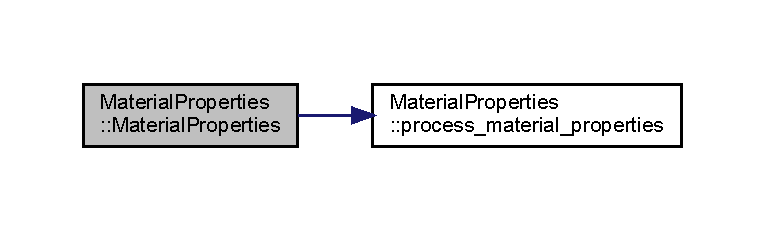
\includegraphics[width=350pt]{class_material_properties_a9c1a2ff5f7cfaacd4b992e96186fbf81_cgraph}
\end{center}
\end{figure}
\mbox{\Hypertarget{class_material_properties_aab94335e9db402f624b88603b233bcab}\label{class_material_properties_aab94335e9db402f624b88603b233bcab}} 
\index{Material\+Properties@{Material\+Properties}!````~Material\+Properties@{$\sim$\+Material\+Properties}}
\index{````~Material\+Properties@{$\sim$\+Material\+Properties}!Material\+Properties@{Material\+Properties}}
\subsubsection{\texorpdfstring{$\sim$\+Material\+Properties()}{~MaterialProperties()}}
{\footnotesize\ttfamily Material\+Properties\+::$\sim$\+Material\+Properties (\begin{DoxyParamCaption}{ }\end{DoxyParamCaption})}



Class destructor. 



Definition at line 17 of file material\+\_\+properties.\+cc.



\subsection{Member Function Documentation}
\mbox{\Hypertarget{class_material_properties_a85d99311c0e1ed1991e79cc6115f0403}\label{class_material_properties_a85d99311c0e1ed1991e79cc6115f0403}} 
\index{Material\+Properties@{Material\+Properties}!get\+\_\+chi\+\_\+nusigf@{get\+\_\+chi\+\_\+nusigf}}
\index{get\+\_\+chi\+\_\+nusigf@{get\+\_\+chi\+\_\+nusigf}!Material\+Properties@{Material\+Properties}}
\subsubsection{\texorpdfstring{get\+\_\+chi\+\_\+nusigf()}{get\_chi\_nusigf()}}
{\footnotesize\ttfamily std\+::vector$<$ std\+::vector$<$ std\+::vector$<$ double $>$ $>$ $>$ Material\+Properties\+::get\+\_\+chi\+\_\+nusigf (\begin{DoxyParamCaption}{ }\end{DoxyParamCaption})}



A function to retrieve all $\chi\nu\sigma_\mathrm{f}$. 



Definition at line 313 of file material\+\_\+properties.\+cc.

\mbox{\Hypertarget{class_material_properties_a262e19465017da2dcd8acb02a2bcd5df}\label{class_material_properties_a262e19465017da2dcd8acb02a2bcd5df}} 
\index{Material\+Properties@{Material\+Properties}!get\+\_\+chi\+\_\+nusigf\+\_\+per\+\_\+ster@{get\+\_\+chi\+\_\+nusigf\+\_\+per\+\_\+ster}}
\index{get\+\_\+chi\+\_\+nusigf\+\_\+per\+\_\+ster@{get\+\_\+chi\+\_\+nusigf\+\_\+per\+\_\+ster}!Material\+Properties@{Material\+Properties}}
\subsubsection{\texorpdfstring{get\+\_\+chi\+\_\+nusigf\+\_\+per\+\_\+ster()}{get\_chi\_nusigf\_per\_ster()}}
{\footnotesize\ttfamily std\+::vector$<$ std\+::vector$<$ std\+::vector$<$ double $>$ $>$ $>$ Material\+Properties\+::get\+\_\+chi\+\_\+nusigf\+\_\+per\+\_\+ster (\begin{DoxyParamCaption}{ }\end{DoxyParamCaption})}



A function to retrieve all $\chi\nu\sigma_\mathrm{f}/(4\pi)$. 



Definition at line 318 of file material\+\_\+properties.\+cc.

\mbox{\Hypertarget{class_material_properties_ae04d6676e685d374cb82a15a6b45d96b}\label{class_material_properties_ae04d6676e685d374cb82a15a6b45d96b}} 
\index{Material\+Properties@{Material\+Properties}!get\+\_\+fissile\+\_\+id\+\_\+map@{get\+\_\+fissile\+\_\+id\+\_\+map}}
\index{get\+\_\+fissile\+\_\+id\+\_\+map@{get\+\_\+fissile\+\_\+id\+\_\+map}!Material\+Properties@{Material\+Properties}}
\subsubsection{\texorpdfstring{get\+\_\+fissile\+\_\+id\+\_\+map()}{get\_fissile\_id\_map()}}
{\footnotesize\ttfamily std\+::unordered\+\_\+map$<$ unsigned int, bool $>$ Material\+Properties\+::get\+\_\+fissile\+\_\+id\+\_\+map (\begin{DoxyParamCaption}{ }\end{DoxyParamCaption})}

A function to retrieve mapping\+: material id-\/$>$if material is fissile boolean.

\begin{DoxyReturn}{Returns}
A Hash table representing the desirable mapping. 
\end{DoxyReturn}


Definition at line 329 of file material\+\_\+properties.\+cc.

\mbox{\Hypertarget{class_material_properties_a319b2dd1caaa13cc9b1afc9ace17e218}\label{class_material_properties_a319b2dd1caaa13cc9b1afc9ace17e218}} 
\index{Material\+Properties@{Material\+Properties}!get\+\_\+inv\+\_\+sigma\+\_\+t@{get\+\_\+inv\+\_\+sigma\+\_\+t}}
\index{get\+\_\+inv\+\_\+sigma\+\_\+t@{get\+\_\+inv\+\_\+sigma\+\_\+t}!Material\+Properties@{Material\+Properties}}
\subsubsection{\texorpdfstring{get\+\_\+inv\+\_\+sigma\+\_\+t()}{get\_inv\_sigma\_t()}}
{\footnotesize\ttfamily std\+::vector$<$ std\+::vector$<$ double $>$ $>$ Material\+Properties\+::get\+\_\+inv\+\_\+sigma\+\_\+t (\begin{DoxyParamCaption}{ }\end{DoxyParamCaption})}



A function to retrieve all $1/\sigma_\mathrm{t}$ for all groups. 



Definition at line 288 of file material\+\_\+properties.\+cc.

\mbox{\Hypertarget{class_material_properties_a75afcc7707f4d77aedf439bacacbfb51}\label{class_material_properties_a75afcc7707f4d77aedf439bacacbfb51}} 
\index{Material\+Properties@{Material\+Properties}!get\+\_\+nusigf@{get\+\_\+nusigf}}
\index{get\+\_\+nusigf@{get\+\_\+nusigf}!Material\+Properties@{Material\+Properties}}
\subsubsection{\texorpdfstring{get\+\_\+nusigf()}{get\_nusigf()}}
{\footnotesize\ttfamily std\+::vector$<$ std\+::vector$<$ double $>$ $>$ Material\+Properties\+::get\+\_\+nusigf (\begin{DoxyParamCaption}{ }\end{DoxyParamCaption})}



A function to retrieve all $\nu\sigma_\mathrm{f}$\textquotesingle{}s. 



Definition at line 323 of file material\+\_\+properties.\+cc.

\mbox{\Hypertarget{class_material_properties_a0bbf8a7d69c73288b015b4247ab0451c}\label{class_material_properties_a0bbf8a7d69c73288b015b4247ab0451c}} 
\index{Material\+Properties@{Material\+Properties}!get\+\_\+q@{get\+\_\+q}}
\index{get\+\_\+q@{get\+\_\+q}!Material\+Properties@{Material\+Properties}}
\subsubsection{\texorpdfstring{get\+\_\+q()}{get\_q()}}
{\footnotesize\ttfamily std\+::vector$<$ std\+::vector$<$ double $>$ $>$ Material\+Properties\+::get\+\_\+q (\begin{DoxyParamCaption}{ }\end{DoxyParamCaption})}



A function to retrieve all fixed source value $Q$\textquotesingle{}s for all groups. 



Definition at line 293 of file material\+\_\+properties.\+cc.

\mbox{\Hypertarget{class_material_properties_a3903e07c80bfe939a3a70be59c74bc53}\label{class_material_properties_a3903e07c80bfe939a3a70be59c74bc53}} 
\index{Material\+Properties@{Material\+Properties}!get\+\_\+q\+\_\+per\+\_\+ster@{get\+\_\+q\+\_\+per\+\_\+ster}}
\index{get\+\_\+q\+\_\+per\+\_\+ster@{get\+\_\+q\+\_\+per\+\_\+ster}!Material\+Properties@{Material\+Properties}}
\subsubsection{\texorpdfstring{get\+\_\+q\+\_\+per\+\_\+ster()}{get\_q\_per\_ster()}}
{\footnotesize\ttfamily std\+::vector$<$ std\+::vector$<$ double $>$ $>$ Material\+Properties\+::get\+\_\+q\+\_\+per\+\_\+ster (\begin{DoxyParamCaption}{ }\end{DoxyParamCaption})}



A function to retrieve all $Q/(4\pi)$\textquotesingle{}s for all groups. 



Definition at line 298 of file material\+\_\+properties.\+cc.

\mbox{\Hypertarget{class_material_properties_a25c7a9ed0b651758dab132bf627c6269}\label{class_material_properties_a25c7a9ed0b651758dab132bf627c6269}} 
\index{Material\+Properties@{Material\+Properties}!get\+\_\+sigma\+\_\+s@{get\+\_\+sigma\+\_\+s}}
\index{get\+\_\+sigma\+\_\+s@{get\+\_\+sigma\+\_\+s}!Material\+Properties@{Material\+Properties}}
\subsubsection{\texorpdfstring{get\+\_\+sigma\+\_\+s()}{get\_sigma\_s()}}
{\footnotesize\ttfamily std\+::vector$<$ std\+::vector$<$ std\+::vector$<$ double $>$ $>$ $>$ Material\+Properties\+::get\+\_\+sigma\+\_\+s (\begin{DoxyParamCaption}{ }\end{DoxyParamCaption})}



A function to retrieve all scattering transfer matrices. 



Definition at line 303 of file material\+\_\+properties.\+cc.

\mbox{\Hypertarget{class_material_properties_a9dbfb1ca140d3b5de3dff2994899182f}\label{class_material_properties_a9dbfb1ca140d3b5de3dff2994899182f}} 
\index{Material\+Properties@{Material\+Properties}!get\+\_\+sigma\+\_\+s\+\_\+per\+\_\+ster@{get\+\_\+sigma\+\_\+s\+\_\+per\+\_\+ster}}
\index{get\+\_\+sigma\+\_\+s\+\_\+per\+\_\+ster@{get\+\_\+sigma\+\_\+s\+\_\+per\+\_\+ster}!Material\+Properties@{Material\+Properties}}
\subsubsection{\texorpdfstring{get\+\_\+sigma\+\_\+s\+\_\+per\+\_\+ster()}{get\_sigma\_s\_per\_ster()}}
{\footnotesize\ttfamily std\+::vector$<$ std\+::vector$<$ std\+::vector$<$ double $>$ $>$ $>$ Material\+Properties\+::get\+\_\+sigma\+\_\+s\+\_\+per\+\_\+ster (\begin{DoxyParamCaption}{ }\end{DoxyParamCaption})}



A function to retrieve all scattering transfer matrices scaled by $4\pi$. 



Definition at line 308 of file material\+\_\+properties.\+cc.

\mbox{\Hypertarget{class_material_properties_ada6ea8094dfc4b5c9610c6dc8d54a47a}\label{class_material_properties_ada6ea8094dfc4b5c9610c6dc8d54a47a}} 
\index{Material\+Properties@{Material\+Properties}!get\+\_\+sigma\+\_\+t@{get\+\_\+sigma\+\_\+t}}
\index{get\+\_\+sigma\+\_\+t@{get\+\_\+sigma\+\_\+t}!Material\+Properties@{Material\+Properties}}
\subsubsection{\texorpdfstring{get\+\_\+sigma\+\_\+t()}{get\_sigma\_t()}}
{\footnotesize\ttfamily std\+::vector$<$ std\+::vector$<$ double $>$ $>$ Material\+Properties\+::get\+\_\+sigma\+\_\+t (\begin{DoxyParamCaption}{ }\end{DoxyParamCaption})}



A function to retrieve all $\sigma_\mathrm{t}$ for all groups. 



Definition at line 283 of file material\+\_\+properties.\+cc.

\mbox{\Hypertarget{class_material_properties_a2a25d8392fb1002f27e048d40f37d627}\label{class_material_properties_a2a25d8392fb1002f27e048d40f37d627}} 
\index{Material\+Properties@{Material\+Properties}!process\+\_\+eigen\+\_\+material\+\_\+properties@{process\+\_\+eigen\+\_\+material\+\_\+properties}}
\index{process\+\_\+eigen\+\_\+material\+\_\+properties@{process\+\_\+eigen\+\_\+material\+\_\+properties}!Material\+Properties@{Material\+Properties}}
\subsubsection{\texorpdfstring{process\+\_\+eigen\+\_\+material\+\_\+properties()}{process\_eigen\_material\_properties()}}
{\footnotesize\ttfamily void Material\+Properties\+::process\+\_\+eigen\+\_\+material\+\_\+properties (\begin{DoxyParamCaption}\item[{Parameter\+Handler \&}]{prm }\end{DoxyParamCaption})\hspace{0.3cm}{\ttfamily [private]}}

Function to process eigenvalue problem specific material properties such as 

Definition at line 165 of file material\+\_\+properties.\+cc.

\mbox{\Hypertarget{class_material_properties_a83121d60325c02dbce98968b45134993}\label{class_material_properties_a83121d60325c02dbce98968b45134993}} 
\index{Material\+Properties@{Material\+Properties}!process\+\_\+material\+\_\+properties@{process\+\_\+material\+\_\+properties}}
\index{process\+\_\+material\+\_\+properties@{process\+\_\+material\+\_\+properties}!Material\+Properties@{Material\+Properties}}
\subsubsection{\texorpdfstring{process\+\_\+material\+\_\+properties()}{process\_material\_properties()}}
{\footnotesize\ttfamily void Material\+Properties\+::process\+\_\+material\+\_\+properties (\begin{DoxyParamCaption}\item[{Parameter\+Handler \&}]{prm }\end{DoxyParamCaption})\hspace{0.3cm}{\ttfamily [private]}}

Function to process all material properties. For eigenvalue problems, it will call this-\/$>$process\+\_\+eigen\+\_\+material\+\_\+properties to process fission-\/related properties.


\begin{DoxyParams}{Parameters}
{\em prm} & Parameter\+Handler object. \\
\hline
\end{DoxyParams}
\begin{DoxyReturn}{Returns}
Void. 
\end{DoxyReturn}


Definition at line 22 of file material\+\_\+properties.\+cc.

Here is the caller graph for this function\+:\nopagebreak
\begin{figure}[H]
\begin{center}
\leavevmode
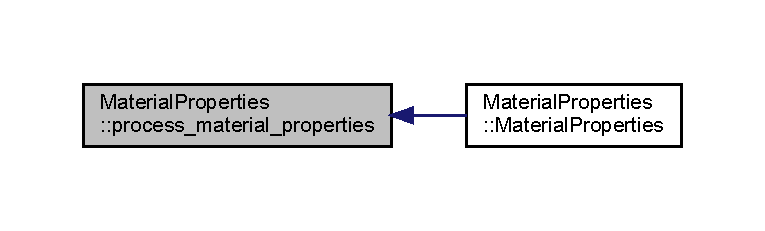
\includegraphics[width=350pt]{class_material_properties_a83121d60325c02dbce98968b45134993_icgraph}
\end{center}
\end{figure}


\subsection{Member Data Documentation}
\mbox{\Hypertarget{class_material_properties_afb25f14545f97c91dacfffcae9d0dcf3}\label{class_material_properties_afb25f14545f97c91dacfffcae9d0dcf3}} 
\index{Material\+Properties@{Material\+Properties}!all\+\_\+chi@{all\+\_\+chi}}
\index{all\+\_\+chi@{all\+\_\+chi}!Material\+Properties@{Material\+Properties}}
\subsubsection{\texorpdfstring{all\+\_\+chi}{all\_chi}}
{\footnotesize\ttfamily std\+::vector$<$std\+::vector$<$double$>$ $>$ Material\+Properties\+::all\+\_\+chi\hspace{0.3cm}{\ttfamily [private]}}

$\chi$ for all materials. A mistake when designing this is that it was treated as other properties. Yet, it is group independent.

\begin{DoxyRefDesc}{Todo}
\item[\hyperlink{todo__todo000008}{Todo}]Change this to std\+::vector$<$double$>$ chi, or using Hash table. \end{DoxyRefDesc}


Definition at line 109 of file material\+\_\+properties.\+h.

\mbox{\Hypertarget{class_material_properties_a77cac1147aa82a264d5d7f8782c6bd26}\label{class_material_properties_a77cac1147aa82a264d5d7f8782c6bd26}} 
\index{Material\+Properties@{Material\+Properties}!all\+\_\+chi\+\_\+nusigf@{all\+\_\+chi\+\_\+nusigf}}
\index{all\+\_\+chi\+\_\+nusigf@{all\+\_\+chi\+\_\+nusigf}!Material\+Properties@{Material\+Properties}}
\subsubsection{\texorpdfstring{all\+\_\+chi\+\_\+nusigf}{all\_chi\_nusigf}}
{\footnotesize\ttfamily std\+::vector$<$std\+::vector$<$std\+::vector$<$double$>$ $>$ $>$ Material\+Properties\+::all\+\_\+chi\+\_\+nusigf\hspace{0.3cm}{\ttfamily [private]}}



$\chi\nu\sigma_\mathrm{f}$ for all materials. 

It is pre-\/computed and transformed into a form of transfer matrix for saving computations. 

Definition at line 131 of file material\+\_\+properties.\+h.

\mbox{\Hypertarget{class_material_properties_a05f7647f245433d8dd164b8538b868fb}\label{class_material_properties_a05f7647f245433d8dd164b8538b868fb}} 
\index{Material\+Properties@{Material\+Properties}!all\+\_\+chi\+\_\+nusigf\+\_\+per\+\_\+ster@{all\+\_\+chi\+\_\+nusigf\+\_\+per\+\_\+ster}}
\index{all\+\_\+chi\+\_\+nusigf\+\_\+per\+\_\+ster@{all\+\_\+chi\+\_\+nusigf\+\_\+per\+\_\+ster}!Material\+Properties@{Material\+Properties}}
\subsubsection{\texorpdfstring{all\+\_\+chi\+\_\+nusigf\+\_\+per\+\_\+ster}{all\_chi\_nusigf\_per\_ster}}
{\footnotesize\ttfamily std\+::vector$<$std\+::vector$<$std\+::vector$<$double$>$ $>$ $>$ Material\+Properties\+::all\+\_\+chi\+\_\+nusigf\+\_\+per\+\_\+ster\hspace{0.3cm}{\ttfamily [private]}}



$\chi\nu\sigma_\mathrm{f}/(4\pi)$ for all materials. 



Definition at line 134 of file material\+\_\+properties.\+h.

\mbox{\Hypertarget{class_material_properties_a9cf448a469e554386e3313d7db0ed4b5}\label{class_material_properties_a9cf448a469e554386e3313d7db0ed4b5}} 
\index{Material\+Properties@{Material\+Properties}!all\+\_\+inv\+\_\+sigt@{all\+\_\+inv\+\_\+sigt}}
\index{all\+\_\+inv\+\_\+sigt@{all\+\_\+inv\+\_\+sigt}!Material\+Properties@{Material\+Properties}}
\subsubsection{\texorpdfstring{all\+\_\+inv\+\_\+sigt}{all\_inv\_sigt}}
{\footnotesize\ttfamily std\+::vector$<$std\+::vector$<$double$>$ $>$ Material\+Properties\+::all\+\_\+inv\+\_\+sigt\hspace{0.3cm}{\ttfamily [private]}}



$1/\sigma_\mathrm{t}$ of all groups for all materials 



Definition at line 101 of file material\+\_\+properties.\+h.

\mbox{\Hypertarget{class_material_properties_ac20f8acc8fb9dd7ef9805eff006f4710}\label{class_material_properties_ac20f8acc8fb9dd7ef9805eff006f4710}} 
\index{Material\+Properties@{Material\+Properties}!all\+\_\+nusigf@{all\+\_\+nusigf}}
\index{all\+\_\+nusigf@{all\+\_\+nusigf}!Material\+Properties@{Material\+Properties}}
\subsubsection{\texorpdfstring{all\+\_\+nusigf}{all\_nusigf}}
{\footnotesize\ttfamily std\+::vector$<$std\+::vector$<$double$>$ $>$ Material\+Properties\+::all\+\_\+nusigf\hspace{0.3cm}{\ttfamily [private]}}



$\nu\sigma_\mathrm{f}$ of all groups for all materials. 



Definition at line 112 of file material\+\_\+properties.\+h.

\mbox{\Hypertarget{class_material_properties_a63087272811561aa476e594b6aa6f4a9}\label{class_material_properties_a63087272811561aa476e594b6aa6f4a9}} 
\index{Material\+Properties@{Material\+Properties}!all\+\_\+q@{all\+\_\+q}}
\index{all\+\_\+q@{all\+\_\+q}!Material\+Properties@{Material\+Properties}}
\subsubsection{\texorpdfstring{all\+\_\+q}{all\_q}}
{\footnotesize\ttfamily std\+::vector$<$std\+::vector$<$double$>$ $>$ Material\+Properties\+::all\+\_\+q\hspace{0.3cm}{\ttfamily [private]}}



Fixed source value $Q$\textquotesingle{}s of all groups for all materials. 



Definition at line 115 of file material\+\_\+properties.\+h.

\mbox{\Hypertarget{class_material_properties_a6ca548f222ef27140c7fc1876c97e6aa}\label{class_material_properties_a6ca548f222ef27140c7fc1876c97e6aa}} 
\index{Material\+Properties@{Material\+Properties}!all\+\_\+q\+\_\+per\+\_\+ster@{all\+\_\+q\+\_\+per\+\_\+ster}}
\index{all\+\_\+q\+\_\+per\+\_\+ster@{all\+\_\+q\+\_\+per\+\_\+ster}!Material\+Properties@{Material\+Properties}}
\subsubsection{\texorpdfstring{all\+\_\+q\+\_\+per\+\_\+ster}{all\_q\_per\_ster}}
{\footnotesize\ttfamily std\+::vector$<$std\+::vector$<$double$>$ $>$ Material\+Properties\+::all\+\_\+q\+\_\+per\+\_\+ster\hspace{0.3cm}{\ttfamily [private]}}



Fixed source value $Q/(4\pi)$\textquotesingle{}s of all groups for all materials. 



Definition at line 118 of file material\+\_\+properties.\+h.

\mbox{\Hypertarget{class_material_properties_a786a421a5a5c61a203b7517e7bafa829}\label{class_material_properties_a786a421a5a5c61a203b7517e7bafa829}} 
\index{Material\+Properties@{Material\+Properties}!all\+\_\+sigs@{all\+\_\+sigs}}
\index{all\+\_\+sigs@{all\+\_\+sigs}!Material\+Properties@{Material\+Properties}}
\subsubsection{\texorpdfstring{all\+\_\+sigs}{all\_sigs}}
{\footnotesize\ttfamily std\+::vector$<$std\+::vector$<$std\+::vector$<$double$>$ $>$ $>$ Material\+Properties\+::all\+\_\+sigs\hspace{0.3cm}{\ttfamily [private]}}



Scattering transfer matrices for all materials. 



Definition at line 121 of file material\+\_\+properties.\+h.

\mbox{\Hypertarget{class_material_properties_a206fc7b81483c3430de643b4dc6598a4}\label{class_material_properties_a206fc7b81483c3430de643b4dc6598a4}} 
\index{Material\+Properties@{Material\+Properties}!all\+\_\+sigs\+\_\+per\+\_\+ster@{all\+\_\+sigs\+\_\+per\+\_\+ster}}
\index{all\+\_\+sigs\+\_\+per\+\_\+ster@{all\+\_\+sigs\+\_\+per\+\_\+ster}!Material\+Properties@{Material\+Properties}}
\subsubsection{\texorpdfstring{all\+\_\+sigs\+\_\+per\+\_\+ster}{all\_sigs\_per\_ster}}
{\footnotesize\ttfamily std\+::vector$<$std\+::vector$<$std\+::vector$<$double$>$ $>$ $>$ Material\+Properties\+::all\+\_\+sigs\+\_\+per\+\_\+ster\hspace{0.3cm}{\ttfamily [private]}}



Scattering transfer matrices scaled by $4\pi$. 



Definition at line 124 of file material\+\_\+properties.\+h.

\mbox{\Hypertarget{class_material_properties_ac2a59b00e3be0e775249354182ae08a4}\label{class_material_properties_ac2a59b00e3be0e775249354182ae08a4}} 
\index{Material\+Properties@{Material\+Properties}!all\+\_\+sigt@{all\+\_\+sigt}}
\index{all\+\_\+sigt@{all\+\_\+sigt}!Material\+Properties@{Material\+Properties}}
\subsubsection{\texorpdfstring{all\+\_\+sigt}{all\_sigt}}
{\footnotesize\ttfamily std\+::vector$<$std\+::vector$<$double$>$ $>$ Material\+Properties\+::all\+\_\+sigt\hspace{0.3cm}{\ttfamily [private]}}



$\sigma_\mathrm{t}$ of all groups for all materials. 



Definition at line 98 of file material\+\_\+properties.\+h.

\mbox{\Hypertarget{class_material_properties_a911d589ba4b11eee87ce5748b760437a}\label{class_material_properties_a911d589ba4b11eee87ce5748b760437a}} 
\index{Material\+Properties@{Material\+Properties}!do\+\_\+nda@{do\+\_\+nda}}
\index{do\+\_\+nda@{do\+\_\+nda}!Material\+Properties@{Material\+Properties}}
\subsubsection{\texorpdfstring{do\+\_\+nda}{do\_nda}}
{\footnotesize\ttfamily bool Material\+Properties\+::do\+\_\+nda\hspace{0.3cm}{\ttfamily [private]}}



Boolean to determine if N\+DA is used. 



Definition at line 88 of file material\+\_\+properties.\+h.

\mbox{\Hypertarget{class_material_properties_a43cff88edebbd4e4f2a012c6639e0b89}\label{class_material_properties_a43cff88edebbd4e4f2a012c6639e0b89}} 
\index{Material\+Properties@{Material\+Properties}!fissile\+\_\+ids@{fissile\+\_\+ids}}
\index{fissile\+\_\+ids@{fissile\+\_\+ids}!Material\+Properties@{Material\+Properties}}
\subsubsection{\texorpdfstring{fissile\+\_\+ids}{fissile\_ids}}
{\footnotesize\ttfamily std\+::unordered\+\_\+set$<$unsigned int$>$ Material\+Properties\+::fissile\+\_\+ids\hspace{0.3cm}{\ttfamily [private]}}



Set of fissile material I\+Ds. 



Definition at line 95 of file material\+\_\+properties.\+h.

\mbox{\Hypertarget{class_material_properties_a2193d0f80fcfbba74a2e84fae0518097}\label{class_material_properties_a2193d0f80fcfbba74a2e84fae0518097}} 
\index{Material\+Properties@{Material\+Properties}!is\+\_\+eigen\+\_\+problem@{is\+\_\+eigen\+\_\+problem}}
\index{is\+\_\+eigen\+\_\+problem@{is\+\_\+eigen\+\_\+problem}!Material\+Properties@{Material\+Properties}}
\subsubsection{\texorpdfstring{is\+\_\+eigen\+\_\+problem}{is\_eigen\_problem}}
{\footnotesize\ttfamily bool Material\+Properties\+::is\+\_\+eigen\+\_\+problem\hspace{0.3cm}{\ttfamily [private]}}



Boolean to determine if it\textquotesingle{}s eigenvalue problem. 



Definition at line 87 of file material\+\_\+properties.\+h.

\mbox{\Hypertarget{class_material_properties_a232e0fa7b96e2d93597e4dd6839b5223}\label{class_material_properties_a232e0fa7b96e2d93597e4dd6839b5223}} 
\index{Material\+Properties@{Material\+Properties}!is\+\_\+material\+\_\+fissile@{is\+\_\+material\+\_\+fissile}}
\index{is\+\_\+material\+\_\+fissile@{is\+\_\+material\+\_\+fissile}!Material\+Properties@{Material\+Properties}}
\subsubsection{\texorpdfstring{is\+\_\+material\+\_\+fissile}{is\_material\_fissile}}
{\footnotesize\ttfamily std\+::unordered\+\_\+map$<$unsigned int, bool$>$ Material\+Properties\+::is\+\_\+material\+\_\+fissile\hspace{0.3cm}{\ttfamily [private]}}



Hash table to determine if a material is fissile. 



Definition at line 93 of file material\+\_\+properties.\+h.

\mbox{\Hypertarget{class_material_properties_a4cae7eee21ea5ed5246765c049caf58b}\label{class_material_properties_a4cae7eee21ea5ed5246765c049caf58b}} 
\index{Material\+Properties@{Material\+Properties}!n\+\_\+group@{n\+\_\+group}}
\index{n\+\_\+group@{n\+\_\+group}!Material\+Properties@{Material\+Properties}}
\subsubsection{\texorpdfstring{n\+\_\+group}{n\_group}}
{\footnotesize\ttfamily unsigned int Material\+Properties\+::n\+\_\+group\hspace{0.3cm}{\ttfamily [private]}}



Number of groups. 



Definition at line 89 of file material\+\_\+properties.\+h.

\mbox{\Hypertarget{class_material_properties_a3bc9713ea94f32fb93d60f2a726e4f2d}\label{class_material_properties_a3bc9713ea94f32fb93d60f2a726e4f2d}} 
\index{Material\+Properties@{Material\+Properties}!n\+\_\+material@{n\+\_\+material}}
\index{n\+\_\+material@{n\+\_\+material}!Material\+Properties@{Material\+Properties}}
\subsubsection{\texorpdfstring{n\+\_\+material}{n\_material}}
{\footnotesize\ttfamily unsigned int Material\+Properties\+::n\+\_\+material\hspace{0.3cm}{\ttfamily [private]}}



Number of materials. 



Definition at line 90 of file material\+\_\+properties.\+h.

\mbox{\Hypertarget{class_material_properties_a28173c461cf9a74c3b0ebe0f51c386d3}\label{class_material_properties_a28173c461cf9a74c3b0ebe0f51c386d3}} 
\index{Material\+Properties@{Material\+Properties}!pi@{pi}}
\index{pi@{pi}!Material\+Properties@{Material\+Properties}}
\subsubsection{\texorpdfstring{pi}{pi}}
{\footnotesize\ttfamily const double Material\+Properties\+::pi\hspace{0.3cm}{\ttfamily [private]}}



3.\+14159... 



Definition at line 85 of file material\+\_\+properties.\+h.



The documentation for this class was generated from the following files\+:\begin{DoxyCompactItemize}
\item 
src/material/\hyperlink{material__properties_8h}{material\+\_\+properties.\+h}\item 
src/material/\hyperlink{material__properties_8cc}{material\+\_\+properties.\+cc}\end{DoxyCompactItemize}

\hypertarget{class_mesh_generator}{}\section{Mesh\+Generator$<$ dim $>$ Class Template Reference}
\label{class_mesh_generator}\index{Mesh\+Generator$<$ dim $>$@{Mesh\+Generator$<$ dim $>$}}


This class provides functionalities to generate a distributed mesh.  




{\ttfamily \#include $<$mesh\+\_\+generator.\+h$>$}

\subsection*{Public Member Functions}
\begin{DoxyCompactItemize}
\item 
\hyperlink{class_mesh_generator_aaf711e4f4d1702dd2f91b8dc3d425765}{Mesh\+Generator} (Parameter\+Handler \&prm)
\item 
\hyperlink{class_mesh_generator_aa8a590f00d9732424e56f54bcc2b6339}{$\sim$\+Mesh\+Generator} ()
\begin{DoxyCompactList}\small\item\em Class destructor. \end{DoxyCompactList}\item 
void \hyperlink{class_mesh_generator_a27c6ff0b0c51700373ef9a1dc10abaaf}{make\+\_\+grid} (parallel\+::distributed\+::\+Triangulation$<$ dim $>$ \&tria)
\item 
void \hyperlink{class_mesh_generator_a0c5f845cf8476424892eb7b263672e73}{get\+\_\+relevant\+\_\+cell\+\_\+iterators} (const Do\+F\+Handler$<$ dim $>$ \&dof\+\_\+handler, std\+::vector$<$ typename Do\+F\+Handler$<$ dim $>$\+::active\+\_\+cell\+\_\+iterator $>$ \&local\+\_\+cells)
\item 
unsigned int \hyperlink{class_mesh_generator_aabb238d5d787e8c9834e4a31d2cc5ea9}{get\+\_\+uniform\+\_\+refinement} ()
\item 
std\+::unordered\+\_\+map$<$ unsigned int, bool $>$ \hyperlink{class_mesh_generator_a525754e676dca1ed4ffac34f63a5d1ae}{get\+\_\+reflective\+\_\+bc\+\_\+map} ()
\end{DoxyCompactItemize}
\subsection*{Private Member Functions}
\begin{DoxyCompactItemize}
\item 
void \hyperlink{class_mesh_generator_a57b433e53fa1b80670a76a1e0c898963}{generate\+\_\+initial\+\_\+grid} (parallel\+::distributed\+::\+Triangulation$<$ dim $>$ \&tria)
\item 
void \hyperlink{class_mesh_generator_a8c0f48b88435360f1209251253912411}{initialize\+\_\+material\+\_\+id} (parallel\+::distributed\+::\+Triangulation$<$ dim $>$ \&tria)
\item 
void \hyperlink{class_mesh_generator_a661d4e5efeb3ee94cc70c5da8e94a0ee}{setup\+\_\+boundary\+\_\+ids} (parallel\+::distributed\+::\+Triangulation$<$ dim $>$ \&tria)
\item 
void \hyperlink{class_mesh_generator_a6d216567b5b599cee526f33d435e6655}{initialize\+\_\+relative\+\_\+position\+\_\+to\+\_\+id\+\_\+map} (Parameter\+Handler \&prm)
\item 
void \hyperlink{class_mesh_generator_a93d10aa06b5b638a859e2fc53dbea5e0}{preprocess\+\_\+reflective\+\_\+bc} (Parameter\+Handler \&prm)
\item 
void \hyperlink{class_mesh_generator_a253330ef901e2a915576f6d6cd4262b5}{process\+\_\+coordinate\+\_\+information} (Parameter\+Handler \&prm)
\item 
void \hyperlink{class_mesh_generator_a9b3414fd31d1d06b0cc4a0c345bc6542}{get\+\_\+cell\+\_\+relative\+\_\+position} (Point$<$ dim $>$ \&position, std\+::vector$<$ unsigned int $>$ \&relative\+\_\+position)
\end{DoxyCompactItemize}
\subsection*{Private Attributes}
\begin{DoxyCompactItemize}
\item 
bool \hyperlink{class_mesh_generator_ad2e8abde741e4c291741cf4ee790e0e2}{is\+\_\+mesh\+\_\+generated}
\item 
bool \hyperlink{class_mesh_generator_a7d6e17f844b8026a062b93ae12b1ee40}{have\+\_\+reflective\+\_\+bc}
\begin{DoxyCompactList}\small\item\em Boolean to determine if reflective BC is used. \end{DoxyCompactList}\item 
std\+::string \hyperlink{class_mesh_generator_a1b283d2ba59b1719cab8dd191e72508a}{mesh\+\_\+filename}
\begin{DoxyCompactList}\small\item\em Mesh filename if mesh is read in. \end{DoxyCompactList}\item 
unsigned int \hyperlink{class_mesh_generator_af8fc6b25c91228ca1ccce7f1c7a2a526}{global\+\_\+refinements}
\begin{DoxyCompactList}\small\item\em Number of global refinements to perform. \end{DoxyCompactList}\item 
std\+::map$<$ std\+::vector$<$ unsigned int $>$, unsigned int $>$ \hyperlink{class_mesh_generator_a4d3e0a3f830a2fa4d35d7f269fba3b02}{relative\+\_\+position\+\_\+to\+\_\+id}
\begin{DoxyCompactList}\small\item\em Mapping\+: cell relative position-\/$>$material ID. \end{DoxyCompactList}\item 
std\+::unordered\+\_\+map$<$ unsigned int, bool $>$ \hyperlink{class_mesh_generator_a5a6820b74d7cef07596e1d28a8bad8aa}{is\+\_\+reflective\+\_\+bc}
\begin{DoxyCompactList}\small\item\em Hash table for the mapping\+: boundary I\+D-\/$>$refl. boundary or not. \end{DoxyCompactList}\item 
std\+::vector$<$ double $>$ \hyperlink{class_mesh_generator_ab65cdce3616c05ca7b02f88a63c7a403}{axis\+\_\+max\+\_\+values}
\begin{DoxyCompactList}\small\item\em Max values per axis in the mesh. \end{DoxyCompactList}\item 
std\+::vector$<$ double $>$ \hyperlink{class_mesh_generator_a55a1699f8cdb9418486af6b0fa3487cc}{cell\+\_\+size\+\_\+all\+\_\+dir}
\begin{DoxyCompactList}\small\item\em Cell length per direction on the coarse mesh. \end{DoxyCompactList}\item 
std\+::vector$<$ unsigned int $>$ \hyperlink{class_mesh_generator_a4d73b2d6a3f66e8a696e2228dc53fb76}{ncell\+\_\+per\+\_\+dir}
\begin{DoxyCompactList}\small\item\em Initial number of cells per axis on the coarse mesh. \end{DoxyCompactList}\end{DoxyCompactItemize}


\subsection{Detailed Description}
\subsubsection*{template$<$int dim$>$\newline
class Mesh\+Generator$<$ dim $>$}

This class provides functionalities to generate a distributed mesh. 

This class implement generating meshes using user-\/defined parameters. Supported functionalities are\+:

(1) Genereate a coarse mesh;

(2) Set up material I\+Ds for all cells in coarse mesh;

(3) Perform global refinements to the mesh.

\begin{DoxyAuthor}{Author}
Weixiong Zheng 
\end{DoxyAuthor}
\begin{DoxyDate}{Date}
2017/05 
\end{DoxyDate}


Definition at line 28 of file mesh\+\_\+generator.\+h.



\subsection{Constructor \& Destructor Documentation}
\mbox{\Hypertarget{class_mesh_generator_aaf711e4f4d1702dd2f91b8dc3d425765}\label{class_mesh_generator_aaf711e4f4d1702dd2f91b8dc3d425765}} 
\index{Mesh\+Generator@{Mesh\+Generator}!Mesh\+Generator@{Mesh\+Generator}}
\index{Mesh\+Generator@{Mesh\+Generator}!Mesh\+Generator@{Mesh\+Generator}}
\subsubsection{\texorpdfstring{Mesh\+Generator()}{MeshGenerator()}}
{\footnotesize\ttfamily template$<$int dim$>$ \\
\hyperlink{class_mesh_generator}{Mesh\+Generator}$<$ dim $>$\+::\hyperlink{class_mesh_generator}{Mesh\+Generator} (\begin{DoxyParamCaption}\item[{Parameter\+Handler \&}]{prm }\end{DoxyParamCaption})}

Class constructor.


\begin{DoxyParams}{Parameters}
{\em prm} & Parameter\+Handler object. \\
\hline
\end{DoxyParams}


Definition at line 12 of file mesh\+\_\+generator.\+cc.

Here is the call graph for this function\+:\nopagebreak
\begin{figure}[H]
\begin{center}
\leavevmode
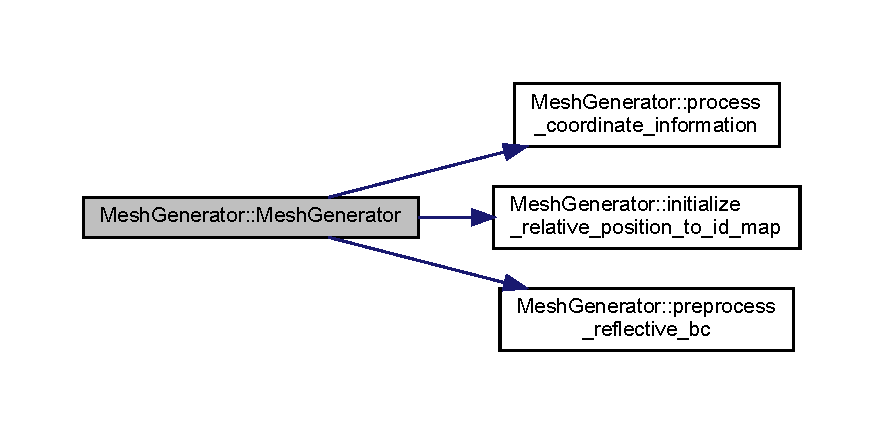
\includegraphics[width=350pt]{class_mesh_generator_aaf711e4f4d1702dd2f91b8dc3d425765_cgraph}
\end{center}
\end{figure}
\mbox{\Hypertarget{class_mesh_generator_aa8a590f00d9732424e56f54bcc2b6339}\label{class_mesh_generator_aa8a590f00d9732424e56f54bcc2b6339}} 
\index{Mesh\+Generator@{Mesh\+Generator}!````~Mesh\+Generator@{$\sim$\+Mesh\+Generator}}
\index{````~Mesh\+Generator@{$\sim$\+Mesh\+Generator}!Mesh\+Generator@{Mesh\+Generator}}
\subsubsection{\texorpdfstring{$\sim$\+Mesh\+Generator()}{~MeshGenerator()}}
{\footnotesize\ttfamily template$<$int dim$>$ \\
\hyperlink{class_mesh_generator}{Mesh\+Generator}$<$ dim $>$\+::$\sim$\hyperlink{class_mesh_generator}{Mesh\+Generator} (\begin{DoxyParamCaption}{ }\end{DoxyParamCaption})}



Class destructor. 



Definition at line 29 of file mesh\+\_\+generator.\+cc.



\subsection{Member Function Documentation}
\mbox{\Hypertarget{class_mesh_generator_a57b433e53fa1b80670a76a1e0c898963}\label{class_mesh_generator_a57b433e53fa1b80670a76a1e0c898963}} 
\index{Mesh\+Generator@{Mesh\+Generator}!generate\+\_\+initial\+\_\+grid@{generate\+\_\+initial\+\_\+grid}}
\index{generate\+\_\+initial\+\_\+grid@{generate\+\_\+initial\+\_\+grid}!Mesh\+Generator@{Mesh\+Generator}}
\subsubsection{\texorpdfstring{generate\+\_\+initial\+\_\+grid()}{generate\_initial\_grid()}}
{\footnotesize\ttfamily template$<$int dim$>$ \\
void \hyperlink{class_mesh_generator}{Mesh\+Generator}$<$ dim $>$\+::generate\+\_\+initial\+\_\+grid (\begin{DoxyParamCaption}\item[{parallel\+::distributed\+::\+Triangulation$<$ dim $>$ \&}]{tria }\end{DoxyParamCaption})\hspace{0.3cm}{\ttfamily [private]}}

Generate initial coarse grid according to user defined parameters. The mesh is a hyer rectangle. In 2D, it is a rectangle. In 3D it is a cuboid. Defining the hyper rectangle requires two diagonal points and mesh cells per axis.


\begin{DoxyParams}{Parameters}
{\em tria} & Triangulation object. \\
\hline
\end{DoxyParams}
\begin{DoxyReturn}{Returns}
Void. Modify tria in place. 
\end{DoxyReturn}


Definition at line 55 of file mesh\+\_\+generator.\+cc.

\mbox{\Hypertarget{class_mesh_generator_a9b3414fd31d1d06b0cc4a0c345bc6542}\label{class_mesh_generator_a9b3414fd31d1d06b0cc4a0c345bc6542}} 
\index{Mesh\+Generator@{Mesh\+Generator}!get\+\_\+cell\+\_\+relative\+\_\+position@{get\+\_\+cell\+\_\+relative\+\_\+position}}
\index{get\+\_\+cell\+\_\+relative\+\_\+position@{get\+\_\+cell\+\_\+relative\+\_\+position}!Mesh\+Generator@{Mesh\+Generator}}
\subsubsection{\texorpdfstring{get\+\_\+cell\+\_\+relative\+\_\+position()}{get\_cell\_relative\_position()}}
{\footnotesize\ttfamily template$<$int dim$>$ \\
void \hyperlink{class_mesh_generator}{Mesh\+Generator}$<$ dim $>$\+::get\+\_\+cell\+\_\+relative\+\_\+position (\begin{DoxyParamCaption}\item[{Point$<$ dim $>$ \&}]{position,  }\item[{std\+::vector$<$ unsigned int $>$ \&}]{relative\+\_\+position }\end{DoxyParamCaption})\hspace{0.3cm}{\ttfamily [private]}}

Get relative position of a cell by providing its center.

\begin{DoxyNote}{Note}
This function will be used only when the mesh is not refined.
\end{DoxyNote}

\begin{DoxyParams}{Parameters}
{\em position} & Cell center. \\
\hline
{\em relateive\+\_\+position} & Relative position of a cell on initial coarse mesh. \\
\hline
\end{DoxyParams}
\begin{DoxyReturn}{Returns}
Void. 
\end{DoxyReturn}


Definition at line 110 of file mesh\+\_\+generator.\+cc.

\mbox{\Hypertarget{class_mesh_generator_a525754e676dca1ed4ffac34f63a5d1ae}\label{class_mesh_generator_a525754e676dca1ed4ffac34f63a5d1ae}} 
\index{Mesh\+Generator@{Mesh\+Generator}!get\+\_\+reflective\+\_\+bc\+\_\+map@{get\+\_\+reflective\+\_\+bc\+\_\+map}}
\index{get\+\_\+reflective\+\_\+bc\+\_\+map@{get\+\_\+reflective\+\_\+bc\+\_\+map}!Mesh\+Generator@{Mesh\+Generator}}
\subsubsection{\texorpdfstring{get\+\_\+reflective\+\_\+bc\+\_\+map()}{get\_reflective\_bc\_map()}}
{\footnotesize\ttfamily template$<$int dim$>$ \\
std\+::unordered\+\_\+map$<$ unsigned int, bool $>$ \hyperlink{class_mesh_generator}{Mesh\+Generator}$<$ dim $>$\+::get\+\_\+reflective\+\_\+bc\+\_\+map (\begin{DoxyParamCaption}{ }\end{DoxyParamCaption})}

Public member function to get Hash table showing if a boundary is reflective.

\begin{DoxyReturn}{Returns}
std\+::unordered\+\_\+map with key as the boundary\+\_\+id (integer) and value as the boolean. 
\end{DoxyReturn}


Definition at line 277 of file mesh\+\_\+generator.\+cc.

\mbox{\Hypertarget{class_mesh_generator_a0c5f845cf8476424892eb7b263672e73}\label{class_mesh_generator_a0c5f845cf8476424892eb7b263672e73}} 
\index{Mesh\+Generator@{Mesh\+Generator}!get\+\_\+relevant\+\_\+cell\+\_\+iterators@{get\+\_\+relevant\+\_\+cell\+\_\+iterators}}
\index{get\+\_\+relevant\+\_\+cell\+\_\+iterators@{get\+\_\+relevant\+\_\+cell\+\_\+iterators}!Mesh\+Generator@{Mesh\+Generator}}
\subsubsection{\texorpdfstring{get\+\_\+relevant\+\_\+cell\+\_\+iterators()}{get\_relevant\_cell\_iterators()}}
{\footnotesize\ttfamily template$<$int dim$>$ \\
void \hyperlink{class_mesh_generator}{Mesh\+Generator}$<$ dim $>$\+::get\+\_\+relevant\+\_\+cell\+\_\+iterators (\begin{DoxyParamCaption}\item[{const Do\+F\+Handler$<$ dim $>$ \&}]{dof\+\_\+handler,  }\item[{std\+::vector$<$ typename Do\+F\+Handler$<$ dim $>$\+::active\+\_\+cell\+\_\+iterator $>$ \&}]{local\+\_\+cells }\end{DoxyParamCaption})}

This function initializes iterators for cells on current processor.


\begin{DoxyParams}{Parameters}
{\em dof\+\_\+handler} & An Do\+F\+Handler object containing iterators of all cells. \\
\hline
{\em local\+\_\+cells} & Vector of active cell iterators living only on current processor. \\
\hline
\end{DoxyParams}
\begin{DoxyReturn}{Returns}
Void. 
\end{DoxyReturn}


Definition at line 229 of file mesh\+\_\+generator.\+cc.

\mbox{\Hypertarget{class_mesh_generator_aabb238d5d787e8c9834e4a31d2cc5ea9}\label{class_mesh_generator_aabb238d5d787e8c9834e4a31d2cc5ea9}} 
\index{Mesh\+Generator@{Mesh\+Generator}!get\+\_\+uniform\+\_\+refinement@{get\+\_\+uniform\+\_\+refinement}}
\index{get\+\_\+uniform\+\_\+refinement@{get\+\_\+uniform\+\_\+refinement}!Mesh\+Generator@{Mesh\+Generator}}
\subsubsection{\texorpdfstring{get\+\_\+uniform\+\_\+refinement()}{get\_uniform\_refinement()}}
{\footnotesize\ttfamily template$<$int dim$>$ \\
unsigned int \hyperlink{class_mesh_generator}{Mesh\+Generator}$<$ dim $>$\+::get\+\_\+uniform\+\_\+refinement (\begin{DoxyParamCaption}{ }\end{DoxyParamCaption})}

Public member function to get total number of global refinements.

\begin{DoxyReturn}{Returns}
Total number of global refinements. 
\end{DoxyReturn}


Definition at line 283 of file mesh\+\_\+generator.\+cc.

\mbox{\Hypertarget{class_mesh_generator_a8c0f48b88435360f1209251253912411}\label{class_mesh_generator_a8c0f48b88435360f1209251253912411}} 
\index{Mesh\+Generator@{Mesh\+Generator}!initialize\+\_\+material\+\_\+id@{initialize\+\_\+material\+\_\+id}}
\index{initialize\+\_\+material\+\_\+id@{initialize\+\_\+material\+\_\+id}!Mesh\+Generator@{Mesh\+Generator}}
\subsubsection{\texorpdfstring{initialize\+\_\+material\+\_\+id()}{initialize\_material\_id()}}
{\footnotesize\ttfamily template$<$int dim$>$ \\
void \hyperlink{class_mesh_generator}{Mesh\+Generator}$<$ dim $>$\+::initialize\+\_\+material\+\_\+id (\begin{DoxyParamCaption}\item[{parallel\+::distributed\+::\+Triangulation$<$ dim $>$ \&}]{tria }\end{DoxyParamCaption})\hspace{0.3cm}{\ttfamily [private]}}

This member function set up material I\+Ds to the cells belonging to current processor on the coarse mesh before performing global refinements.


\begin{DoxyParams}{Parameters}
{\em tria} & Triangulation object. \\
\hline
\end{DoxyParams}
\begin{DoxyReturn}{Returns}
Void. Modify tria in place. 
\end{DoxyReturn}


Definition at line 93 of file mesh\+\_\+generator.\+cc.

\mbox{\Hypertarget{class_mesh_generator_a6d216567b5b599cee526f33d435e6655}\label{class_mesh_generator_a6d216567b5b599cee526f33d435e6655}} 
\index{Mesh\+Generator@{Mesh\+Generator}!initialize\+\_\+relative\+\_\+position\+\_\+to\+\_\+id\+\_\+map@{initialize\+\_\+relative\+\_\+position\+\_\+to\+\_\+id\+\_\+map}}
\index{initialize\+\_\+relative\+\_\+position\+\_\+to\+\_\+id\+\_\+map@{initialize\+\_\+relative\+\_\+position\+\_\+to\+\_\+id\+\_\+map}!Mesh\+Generator@{Mesh\+Generator}}
\subsubsection{\texorpdfstring{initialize\+\_\+relative\+\_\+position\+\_\+to\+\_\+id\+\_\+map()}{initialize\_relative\_position\_to\_id\_map()}}
{\footnotesize\ttfamily template$<$int dim$>$ \\
void \hyperlink{class_mesh_generator}{Mesh\+Generator}$<$ dim $>$\+::initialize\+\_\+relative\+\_\+position\+\_\+to\+\_\+id\+\_\+map (\begin{DoxyParamCaption}\item[{Parameter\+Handler \&}]{prm }\end{DoxyParamCaption})\hspace{0.3cm}{\ttfamily [private]}}

Function to initialize the mapping\+: cell relative pos.-\/$>$material ID on initial mesh.


\begin{DoxyParams}{Parameters}
{\em prm} & Parameter\+Handler object. \\
\hline
\end{DoxyParams}
\begin{DoxyReturn}{Returns}
Void. 
\end{DoxyReturn}


Definition at line 240 of file mesh\+\_\+generator.\+cc.

Here is the caller graph for this function\+:\nopagebreak
\begin{figure}[H]
\begin{center}
\leavevmode
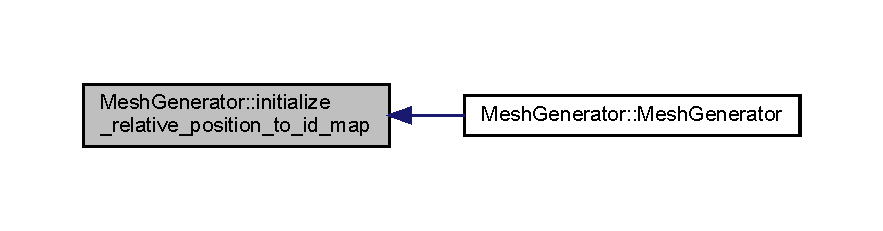
\includegraphics[width=350pt]{class_mesh_generator_a6d216567b5b599cee526f33d435e6655_icgraph}
\end{center}
\end{figure}
\mbox{\Hypertarget{class_mesh_generator_a27c6ff0b0c51700373ef9a1dc10abaaf}\label{class_mesh_generator_a27c6ff0b0c51700373ef9a1dc10abaaf}} 
\index{Mesh\+Generator@{Mesh\+Generator}!make\+\_\+grid@{make\+\_\+grid}}
\index{make\+\_\+grid@{make\+\_\+grid}!Mesh\+Generator@{Mesh\+Generator}}
\subsubsection{\texorpdfstring{make\+\_\+grid()}{make\_grid()}}
{\footnotesize\ttfamily template$<$int dim$>$ \\
void \hyperlink{class_mesh_generator}{Mesh\+Generator}$<$ dim $>$\+::make\+\_\+grid (\begin{DoxyParamCaption}\item[{parallel\+::distributed\+::\+Triangulation$<$ dim $>$ \&}]{tria }\end{DoxyParamCaption})}

This function generates or reads in coarse mesh without global refinements. Currently, read-\/in is not fully implemented yet.

\begin{DoxyNote}{Note}
There is unknown error if total number of cells in the coarse mesh cannot be divided by number of processors.
\end{DoxyNote}
\begin{DoxyRefDesc}{Todo}
\item[\hyperlink{todo__todo000006}{Todo}]Add functionality to read in meshes.\end{DoxyRefDesc}



\begin{DoxyParams}{Parameters}
{\em tria} & Triangulation object. \\
\hline
\end{DoxyParams}
\begin{DoxyReturn}{Returns}
Void. Modify tria in place. 
\end{DoxyReturn}


Definition at line 35 of file mesh\+\_\+generator.\+cc.

\mbox{\Hypertarget{class_mesh_generator_a93d10aa06b5b638a859e2fc53dbea5e0}\label{class_mesh_generator_a93d10aa06b5b638a859e2fc53dbea5e0}} 
\index{Mesh\+Generator@{Mesh\+Generator}!preprocess\+\_\+reflective\+\_\+bc@{preprocess\+\_\+reflective\+\_\+bc}}
\index{preprocess\+\_\+reflective\+\_\+bc@{preprocess\+\_\+reflective\+\_\+bc}!Mesh\+Generator@{Mesh\+Generator}}
\subsubsection{\texorpdfstring{preprocess\+\_\+reflective\+\_\+bc()}{preprocess\_reflective\_bc()}}
{\footnotesize\ttfamily template$<$int dim$>$ \\
void \hyperlink{class_mesh_generator}{Mesh\+Generator}$<$ dim $>$\+::preprocess\+\_\+reflective\+\_\+bc (\begin{DoxyParamCaption}\item[{Parameter\+Handler \&}]{prm }\end{DoxyParamCaption})\hspace{0.3cm}{\ttfamily [private]}}

A function to establish the mapping\+: boundary id-\/$>$refl. BC or not.


\begin{DoxyParams}{Parameters}
{\em prm} & Parameter\+Handler object. \\
\hline
\end{DoxyParams}


Definition at line 196 of file mesh\+\_\+generator.\+cc.

Here is the caller graph for this function\+:\nopagebreak
\begin{figure}[H]
\begin{center}
\leavevmode
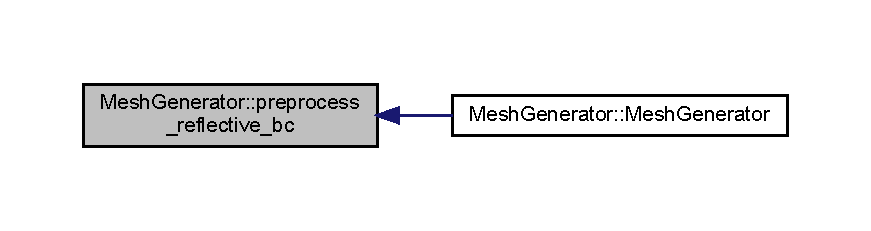
\includegraphics[width=350pt]{class_mesh_generator_a93d10aa06b5b638a859e2fc53dbea5e0_icgraph}
\end{center}
\end{figure}
\mbox{\Hypertarget{class_mesh_generator_a253330ef901e2a915576f6d6cd4262b5}\label{class_mesh_generator_a253330ef901e2a915576f6d6cd4262b5}} 
\index{Mesh\+Generator@{Mesh\+Generator}!process\+\_\+coordinate\+\_\+information@{process\+\_\+coordinate\+\_\+information}}
\index{process\+\_\+coordinate\+\_\+information@{process\+\_\+coordinate\+\_\+information}!Mesh\+Generator@{Mesh\+Generator}}
\subsubsection{\texorpdfstring{process\+\_\+coordinate\+\_\+information()}{process\_coordinate\_information()}}
{\footnotesize\ttfamily template$<$int dim$>$ \\
void \hyperlink{class_mesh_generator}{Mesh\+Generator}$<$ dim $>$\+::process\+\_\+coordinate\+\_\+information (\begin{DoxyParamCaption}\item[{Parameter\+Handler \&}]{prm }\end{DoxyParamCaption})\hspace{0.3cm}{\ttfamily [private]}}

A function to process coordinate info such as axis lengths, cell number per axis on initial mesh etc.


\begin{DoxyParams}{Parameters}
{\em prm} & Parameter\+Handler object. \\
\hline
\end{DoxyParams}
\begin{DoxyReturn}{Returns}
Void. 
\end{DoxyReturn}


Definition at line 171 of file mesh\+\_\+generator.\+cc.

Here is the caller graph for this function\+:\nopagebreak
\begin{figure}[H]
\begin{center}
\leavevmode
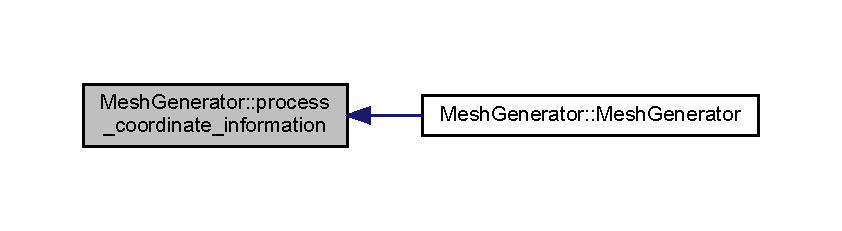
\includegraphics[width=350pt]{class_mesh_generator_a253330ef901e2a915576f6d6cd4262b5_icgraph}
\end{center}
\end{figure}
\mbox{\Hypertarget{class_mesh_generator_a661d4e5efeb3ee94cc70c5da8e94a0ee}\label{class_mesh_generator_a661d4e5efeb3ee94cc70c5da8e94a0ee}} 
\index{Mesh\+Generator@{Mesh\+Generator}!setup\+\_\+boundary\+\_\+ids@{setup\+\_\+boundary\+\_\+ids}}
\index{setup\+\_\+boundary\+\_\+ids@{setup\+\_\+boundary\+\_\+ids}!Mesh\+Generator@{Mesh\+Generator}}
\subsubsection{\texorpdfstring{setup\+\_\+boundary\+\_\+ids()}{setup\_boundary\_ids()}}
{\footnotesize\ttfamily template$<$int dim$>$ \\
void \hyperlink{class_mesh_generator}{Mesh\+Generator}$<$ dim $>$\+::setup\+\_\+boundary\+\_\+ids (\begin{DoxyParamCaption}\item[{parallel\+::distributed\+::\+Triangulation$<$ dim $>$ \&}]{tria }\end{DoxyParamCaption})\hspace{0.3cm}{\ttfamily [private]}}

This function set up boundary I\+Ds. The naming philosophy is xmin-\/$>$0, xmax-\/$>$1, ymin-\/$>$2, ymax-\/$>$3, zmin-\/$>$4, zmax-\/$>$5 if boundaries are applicable.


\begin{DoxyParams}{Parameters}
{\em tria} & Triangulation object. \\
\hline
\end{DoxyParams}
\begin{DoxyReturn}{Returns}
Void. Modify tria in place. 
\end{DoxyReturn}


Definition at line 129 of file mesh\+\_\+generator.\+cc.



\subsection{Member Data Documentation}
\mbox{\Hypertarget{class_mesh_generator_ab65cdce3616c05ca7b02f88a63c7a403}\label{class_mesh_generator_ab65cdce3616c05ca7b02f88a63c7a403}} 
\index{Mesh\+Generator@{Mesh\+Generator}!axis\+\_\+max\+\_\+values@{axis\+\_\+max\+\_\+values}}
\index{axis\+\_\+max\+\_\+values@{axis\+\_\+max\+\_\+values}!Mesh\+Generator@{Mesh\+Generator}}
\subsubsection{\texorpdfstring{axis\+\_\+max\+\_\+values}{axis\_max\_values}}
{\footnotesize\ttfamily template$<$int dim$>$ \\
std\+::vector$<$double$>$ \hyperlink{class_mesh_generator}{Mesh\+Generator}$<$ dim $>$\+::axis\+\_\+max\+\_\+values\hspace{0.3cm}{\ttfamily [private]}}



Max values per axis in the mesh. 



Definition at line 164 of file mesh\+\_\+generator.\+h.

\mbox{\Hypertarget{class_mesh_generator_a55a1699f8cdb9418486af6b0fa3487cc}\label{class_mesh_generator_a55a1699f8cdb9418486af6b0fa3487cc}} 
\index{Mesh\+Generator@{Mesh\+Generator}!cell\+\_\+size\+\_\+all\+\_\+dir@{cell\+\_\+size\+\_\+all\+\_\+dir}}
\index{cell\+\_\+size\+\_\+all\+\_\+dir@{cell\+\_\+size\+\_\+all\+\_\+dir}!Mesh\+Generator@{Mesh\+Generator}}
\subsubsection{\texorpdfstring{cell\+\_\+size\+\_\+all\+\_\+dir}{cell\_size\_all\_dir}}
{\footnotesize\ttfamily template$<$int dim$>$ \\
std\+::vector$<$double$>$ \hyperlink{class_mesh_generator}{Mesh\+Generator}$<$ dim $>$\+::cell\+\_\+size\+\_\+all\+\_\+dir\hspace{0.3cm}{\ttfamily [private]}}



Cell length per direction on the coarse mesh. 



Definition at line 165 of file mesh\+\_\+generator.\+h.

\mbox{\Hypertarget{class_mesh_generator_af8fc6b25c91228ca1ccce7f1c7a2a526}\label{class_mesh_generator_af8fc6b25c91228ca1ccce7f1c7a2a526}} 
\index{Mesh\+Generator@{Mesh\+Generator}!global\+\_\+refinements@{global\+\_\+refinements}}
\index{global\+\_\+refinements@{global\+\_\+refinements}!Mesh\+Generator@{Mesh\+Generator}}
\subsubsection{\texorpdfstring{global\+\_\+refinements}{global\_refinements}}
{\footnotesize\ttfamily template$<$int dim$>$ \\
unsigned int \hyperlink{class_mesh_generator}{Mesh\+Generator}$<$ dim $>$\+::global\+\_\+refinements\hspace{0.3cm}{\ttfamily [private]}}



Number of global refinements to perform. 



Definition at line 156 of file mesh\+\_\+generator.\+h.

\mbox{\Hypertarget{class_mesh_generator_a7d6e17f844b8026a062b93ae12b1ee40}\label{class_mesh_generator_a7d6e17f844b8026a062b93ae12b1ee40}} 
\index{Mesh\+Generator@{Mesh\+Generator}!have\+\_\+reflective\+\_\+bc@{have\+\_\+reflective\+\_\+bc}}
\index{have\+\_\+reflective\+\_\+bc@{have\+\_\+reflective\+\_\+bc}!Mesh\+Generator@{Mesh\+Generator}}
\subsubsection{\texorpdfstring{have\+\_\+reflective\+\_\+bc}{have\_reflective\_bc}}
{\footnotesize\ttfamily template$<$int dim$>$ \\
bool \hyperlink{class_mesh_generator}{Mesh\+Generator}$<$ dim $>$\+::have\+\_\+reflective\+\_\+bc\hspace{0.3cm}{\ttfamily [private]}}



Boolean to determine if reflective BC is used. 



Definition at line 154 of file mesh\+\_\+generator.\+h.

\mbox{\Hypertarget{class_mesh_generator_ad2e8abde741e4c291741cf4ee790e0e2}\label{class_mesh_generator_ad2e8abde741e4c291741cf4ee790e0e2}} 
\index{Mesh\+Generator@{Mesh\+Generator}!is\+\_\+mesh\+\_\+generated@{is\+\_\+mesh\+\_\+generated}}
\index{is\+\_\+mesh\+\_\+generated@{is\+\_\+mesh\+\_\+generated}!Mesh\+Generator@{Mesh\+Generator}}
\subsubsection{\texorpdfstring{is\+\_\+mesh\+\_\+generated}{is\_mesh\_generated}}
{\footnotesize\ttfamily template$<$int dim$>$ \\
bool \hyperlink{class_mesh_generator}{Mesh\+Generator}$<$ dim $>$\+::is\+\_\+mesh\+\_\+generated\hspace{0.3cm}{\ttfamily [private]}}

Boolean to determine if mesh needs to be generated or read-\/in. Currently, B\+A\+RT can only use generated mesh and read-\/in functionality is not fully developed. 

Definition at line 153 of file mesh\+\_\+generator.\+h.

\mbox{\Hypertarget{class_mesh_generator_a5a6820b74d7cef07596e1d28a8bad8aa}\label{class_mesh_generator_a5a6820b74d7cef07596e1d28a8bad8aa}} 
\index{Mesh\+Generator@{Mesh\+Generator}!is\+\_\+reflective\+\_\+bc@{is\+\_\+reflective\+\_\+bc}}
\index{is\+\_\+reflective\+\_\+bc@{is\+\_\+reflective\+\_\+bc}!Mesh\+Generator@{Mesh\+Generator}}
\subsubsection{\texorpdfstring{is\+\_\+reflective\+\_\+bc}{is\_reflective\_bc}}
{\footnotesize\ttfamily template$<$int dim$>$ \\
std\+::unordered\+\_\+map$<$unsigned int, bool$>$ \hyperlink{class_mesh_generator}{Mesh\+Generator}$<$ dim $>$\+::is\+\_\+reflective\+\_\+bc\hspace{0.3cm}{\ttfamily [private]}}



Hash table for the mapping\+: boundary I\+D-\/$>$refl. boundary or not. 



Definition at line 162 of file mesh\+\_\+generator.\+h.

\mbox{\Hypertarget{class_mesh_generator_a1b283d2ba59b1719cab8dd191e72508a}\label{class_mesh_generator_a1b283d2ba59b1719cab8dd191e72508a}} 
\index{Mesh\+Generator@{Mesh\+Generator}!mesh\+\_\+filename@{mesh\+\_\+filename}}
\index{mesh\+\_\+filename@{mesh\+\_\+filename}!Mesh\+Generator@{Mesh\+Generator}}
\subsubsection{\texorpdfstring{mesh\+\_\+filename}{mesh\_filename}}
{\footnotesize\ttfamily template$<$int dim$>$ \\
std\+::string \hyperlink{class_mesh_generator}{Mesh\+Generator}$<$ dim $>$\+::mesh\+\_\+filename\hspace{0.3cm}{\ttfamily [private]}}



Mesh filename if mesh is read in. 



Definition at line 155 of file mesh\+\_\+generator.\+h.

\mbox{\Hypertarget{class_mesh_generator_a4d73b2d6a3f66e8a696e2228dc53fb76}\label{class_mesh_generator_a4d73b2d6a3f66e8a696e2228dc53fb76}} 
\index{Mesh\+Generator@{Mesh\+Generator}!ncell\+\_\+per\+\_\+dir@{ncell\+\_\+per\+\_\+dir}}
\index{ncell\+\_\+per\+\_\+dir@{ncell\+\_\+per\+\_\+dir}!Mesh\+Generator@{Mesh\+Generator}}
\subsubsection{\texorpdfstring{ncell\+\_\+per\+\_\+dir}{ncell\_per\_dir}}
{\footnotesize\ttfamily template$<$int dim$>$ \\
std\+::vector$<$unsigned int$>$ \hyperlink{class_mesh_generator}{Mesh\+Generator}$<$ dim $>$\+::ncell\+\_\+per\+\_\+dir\hspace{0.3cm}{\ttfamily [private]}}



Initial number of cells per axis on the coarse mesh. 



Definition at line 166 of file mesh\+\_\+generator.\+h.

\mbox{\Hypertarget{class_mesh_generator_a4d3e0a3f830a2fa4d35d7f269fba3b02}\label{class_mesh_generator_a4d3e0a3f830a2fa4d35d7f269fba3b02}} 
\index{Mesh\+Generator@{Mesh\+Generator}!relative\+\_\+position\+\_\+to\+\_\+id@{relative\+\_\+position\+\_\+to\+\_\+id}}
\index{relative\+\_\+position\+\_\+to\+\_\+id@{relative\+\_\+position\+\_\+to\+\_\+id}!Mesh\+Generator@{Mesh\+Generator}}
\subsubsection{\texorpdfstring{relative\+\_\+position\+\_\+to\+\_\+id}{relative\_position\_to\_id}}
{\footnotesize\ttfamily template$<$int dim$>$ \\
std\+::map$<$std\+::vector$<$unsigned int$>$, unsigned int$>$ \hyperlink{class_mesh_generator}{Mesh\+Generator}$<$ dim $>$\+::relative\+\_\+position\+\_\+to\+\_\+id\hspace{0.3cm}{\ttfamily [private]}}



Mapping\+: cell relative position-\/$>$material ID. 



Definition at line 159 of file mesh\+\_\+generator.\+h.



The documentation for this class was generated from the following files\+:\begin{DoxyCompactItemize}
\item 
src/mesh/\hyperlink{mesh__generator_8h}{mesh\+\_\+generator.\+h}\item 
src/mesh/\hyperlink{mesh__generator_8cc}{mesh\+\_\+generator.\+cc}\end{DoxyCompactItemize}

\hypertarget{class_m_g_base}{}\section{M\+G\+Base$<$ dim $>$ Class Template Reference}
\label{class_m_g_base}\index{M\+G\+Base$<$ dim $>$@{M\+G\+Base$<$ dim $>$}}


This class provides abstract functionalities for MG calculations.  




{\ttfamily \#include $<$mg\+\_\+base.\+h$>$}



Inheritance diagram for M\+G\+Base$<$ dim $>$\+:\nopagebreak
\begin{figure}[H]
\begin{center}
\leavevmode
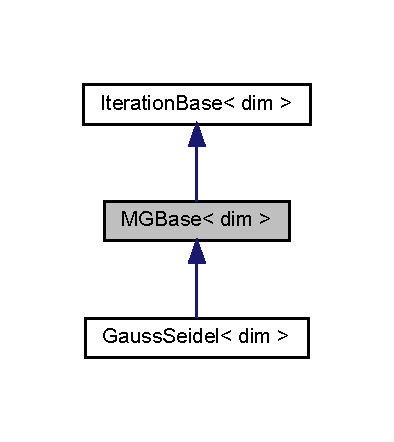
\includegraphics[width=189pt]{class_m_g_base__inherit__graph}
\end{center}
\end{figure}


Collaboration diagram for M\+G\+Base$<$ dim $>$\+:\nopagebreak
\begin{figure}[H]
\begin{center}
\leavevmode
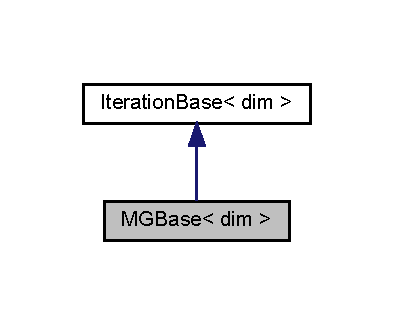
\includegraphics[width=189pt]{class_m_g_base__coll__graph}
\end{center}
\end{figure}
\subsection*{Public Member Functions}
\begin{DoxyCompactItemize}
\item 
\hyperlink{class_m_g_base_ad938184229e773a339be9ba1fc487aa1}{M\+G\+Base} (const Parameter\+Handler \&prm)
\item 
virtual \hyperlink{class_m_g_base_a011e50e1caf44cfa3335b95d161ba14d}{$\sim$\+M\+G\+Base} ()
\begin{DoxyCompactList}\small\item\em A virtual destructor for M\+G\+Base. \end{DoxyCompactList}\item 
virtual void \hyperlink{class_m_g_base_a3586c47d901608bc42792c6de456b1cb}{do\+\_\+iterations} (std\+::vector$<$ Vector$<$ double $>$ $>$ \&sflxes\+\_\+proc, std\+::vector$<$ std\+\_\+cxx11\+::shared\+\_\+ptr$<$ \hyperlink{class_equation_base}{Equation\+Base}$<$ dim $>$ $>$ $>$ \&equ\+\_\+ptrs, std\+\_\+cxx11\+::shared\+\_\+ptr$<$ \hyperlink{class_i_g_base}{I\+G\+Base}$<$ dim $>$ $>$ ig\+\_\+ptr)
\item 
virtual void \hyperlink{class_m_g_base_a6ae523b6ee434588d85f8370413d0de9}{mg\+\_\+iterations} (std\+::vector$<$ Vector$<$ double $>$ $>$ \&sflxes\+\_\+proc, std\+::vector$<$ std\+\_\+cxx11\+::shared\+\_\+ptr$<$ \hyperlink{class_equation_base}{Equation\+Base}$<$ dim $>$ $>$ $>$ \&equ\+\_\+ptrs, std\+\_\+cxx11\+::shared\+\_\+ptr$<$ \hyperlink{class_i_g_base}{I\+G\+Base}$<$ dim $>$ $>$ ig\+\_\+ptr)
\item 
virtual void \hyperlink{class_m_g_base_a55ba9bef3616dd5eab9e3986f6e8e311}{nonthermal\+\_\+solves} (std\+::vector$<$ Vector$<$ double $>$ $>$ \&sflxes\+\_\+proc, std\+::vector$<$ std\+\_\+cxx11\+::shared\+\_\+ptr$<$ \hyperlink{class_equation_base}{Equation\+Base}$<$ dim $>$ $>$ $>$ \&equ\+\_\+ptrs, std\+\_\+cxx11\+::shared\+\_\+ptr$<$ \hyperlink{class_i_g_base}{I\+G\+Base}$<$ dim $>$ $>$ ig\+\_\+ptr)
\item 
virtual void \hyperlink{class_m_g_base_a9d3c6ab6e58f0119badb30feedb2ac4d}{thermal\+\_\+iterations} (std\+::vector$<$ Vector$<$ double $>$ $>$ \&sflxes\+\_\+proc, std\+::vector$<$ std\+\_\+cxx11\+::shared\+\_\+ptr$<$ \hyperlink{class_equation_base}{Equation\+Base}$<$ dim $>$ $>$ $>$ \&equ\+\_\+ptrs, std\+\_\+cxx11\+::shared\+\_\+ptr$<$ \hyperlink{class_i_g_base}{I\+G\+Base}$<$ dim $>$ $>$ ig\+\_\+ptr)
\end{DoxyCompactItemize}
\subsection*{Protected Attributes}
\begin{DoxyCompactItemize}
\item 
unsigned int \hyperlink{class_m_g_base_a7df1f6ce51cf6eb033420be98b1f0019}{g\+\_\+thermal}
\begin{DoxyCompactList}\small\item\em Starting group index where upscattering exists. \end{DoxyCompactList}\item 
const double \hyperlink{class_m_g_base_af50b1bdc92270c342524eacfc644170c}{err\+\_\+phi\+\_\+tol}
\begin{DoxyCompactList}\small\item\em Multigroup iteration tolerance for convergence check. \end{DoxyCompactList}\item 
std\+::vector$<$ Vector$<$ double $>$ $>$ \hyperlink{class_m_g_base_ad8a9d4163bb31470fff74fe787c23788}{sflxes\+\_\+proc\+\_\+prev\+\_\+mg}
\begin{DoxyCompactList}\small\item\em A scalar flux vector recording the old sflxes\+\_\+proc. \end{DoxyCompactList}\end{DoxyCompactItemize}
\subsection*{Additional Inherited Members}


\subsection{Detailed Description}
\subsubsection*{template$<$int dim$>$\newline
class M\+G\+Base$<$ dim $>$}

This class provides abstract functionalities for MG calculations. 

This class serves as the base class of MG iterations. It inherits from Iteration\+Base.

\begin{DoxyAuthor}{Author}
Weixiong Zheng 
\end{DoxyAuthor}
\begin{DoxyDate}{Date}
2017/08 
\end{DoxyDate}


Definition at line 18 of file mg\+\_\+base.\+h.



\subsection{Constructor \& Destructor Documentation}
\mbox{\Hypertarget{class_m_g_base_ad938184229e773a339be9ba1fc487aa1}\label{class_m_g_base_ad938184229e773a339be9ba1fc487aa1}} 
\index{M\+G\+Base@{M\+G\+Base}!M\+G\+Base@{M\+G\+Base}}
\index{M\+G\+Base@{M\+G\+Base}!M\+G\+Base@{M\+G\+Base}}
\subsubsection{\texorpdfstring{M\+G\+Base()}{MGBase()}}
{\footnotesize\ttfamily template$<$int dim$>$ \\
\hyperlink{class_m_g_base}{M\+G\+Base}$<$ dim $>$\+::\hyperlink{class_m_g_base}{M\+G\+Base} (\begin{DoxyParamCaption}\item[{const Parameter\+Handler \&}]{prm }\end{DoxyParamCaption})}

A constructor of M\+G\+Base.


\begin{DoxyParams}{Parameters}
{\em prm} & A Parameter\+Handler object containing all the parameters needed. \\
\hline
\end{DoxyParams}


Definition at line 4 of file mg\+\_\+base.\+cc.

\mbox{\Hypertarget{class_m_g_base_a011e50e1caf44cfa3335b95d161ba14d}\label{class_m_g_base_a011e50e1caf44cfa3335b95d161ba14d}} 
\index{M\+G\+Base@{M\+G\+Base}!````~M\+G\+Base@{$\sim$\+M\+G\+Base}}
\index{````~M\+G\+Base@{$\sim$\+M\+G\+Base}!M\+G\+Base@{M\+G\+Base}}
\subsubsection{\texorpdfstring{$\sim$\+M\+G\+Base()}{~MGBase()}}
{\footnotesize\ttfamily template$<$int dim$>$ \\
\hyperlink{class_m_g_base}{M\+G\+Base}$<$ dim $>$\+::$\sim$\hyperlink{class_m_g_base}{M\+G\+Base} (\begin{DoxyParamCaption}{ }\end{DoxyParamCaption})\hspace{0.3cm}{\ttfamily [virtual]}}



A virtual destructor for M\+G\+Base. 



Definition at line 18 of file mg\+\_\+base.\+cc.



\subsection{Member Function Documentation}
\mbox{\Hypertarget{class_m_g_base_a3586c47d901608bc42792c6de456b1cb}\label{class_m_g_base_a3586c47d901608bc42792c6de456b1cb}} 
\index{M\+G\+Base@{M\+G\+Base}!do\+\_\+iterations@{do\+\_\+iterations}}
\index{do\+\_\+iterations@{do\+\_\+iterations}!M\+G\+Base@{M\+G\+Base}}
\subsubsection{\texorpdfstring{do\+\_\+iterations()}{do\_iterations()}}
{\footnotesize\ttfamily template$<$int dim$>$ \\
void \hyperlink{class_m_g_base}{M\+G\+Base}$<$ dim $>$\+::do\+\_\+iterations (\begin{DoxyParamCaption}\item[{std\+::vector$<$ Vector$<$ double $>$ $>$ \&}]{sflxes\+\_\+proc,  }\item[{std\+::vector$<$ std\+\_\+cxx11\+::shared\+\_\+ptr$<$ \hyperlink{class_equation_base}{Equation\+Base}$<$ dim $>$ $>$ $>$ \&}]{equ\+\_\+ptrs,  }\item[{std\+\_\+cxx11\+::shared\+\_\+ptr$<$ \hyperlink{class_i_g_base}{I\+G\+Base}$<$ dim $>$ $>$}]{ig\+\_\+ptr }\end{DoxyParamCaption})\hspace{0.3cm}{\ttfamily [virtual]}}

This function will call mg\+\_\+iterations to perform MG iterations in fixed source problems. This function shall not be called in eigenvalue calculations.

\begin{DoxyRefDesc}{Todo}
\item[\hyperlink{todo__todo000005}{Todo}]Implement N\+DA scheme in this function.\end{DoxyRefDesc}



\begin{DoxyParams}{Parameters}
{\em sflxes\+\_\+proc} & A vector of scalar fluxes for all groups. \\
\hline
{\em equ\+\_\+ptrs} & A vector of shared\+\_\+ptr\textquotesingle{}s of Equation\+Base objects. \\
\hline
{\em ig\+\_\+ptr} & A shared\+\_\+ptr of I\+G\+Base$<$dim$>$ object. \\
\hline
\end{DoxyParams}
\begin{DoxyReturn}{Returns}
Void. 
\end{DoxyReturn}


Definition at line 24 of file mg\+\_\+base.\+cc.

\mbox{\Hypertarget{class_m_g_base_a6ae523b6ee434588d85f8370413d0de9}\label{class_m_g_base_a6ae523b6ee434588d85f8370413d0de9}} 
\index{M\+G\+Base@{M\+G\+Base}!mg\+\_\+iterations@{mg\+\_\+iterations}}
\index{mg\+\_\+iterations@{mg\+\_\+iterations}!M\+G\+Base@{M\+G\+Base}}
\subsubsection{\texorpdfstring{mg\+\_\+iterations()}{mg\_iterations()}}
{\footnotesize\ttfamily template$<$int dim$>$ \\
void \hyperlink{class_m_g_base}{M\+G\+Base}$<$ dim $>$\+::mg\+\_\+iterations (\begin{DoxyParamCaption}\item[{std\+::vector$<$ Vector$<$ double $>$ $>$ \&}]{sflxes\+\_\+proc,  }\item[{std\+::vector$<$ std\+\_\+cxx11\+::shared\+\_\+ptr$<$ \hyperlink{class_equation_base}{Equation\+Base}$<$ dim $>$ $>$ $>$ \&}]{equ\+\_\+ptrs,  }\item[{std\+\_\+cxx11\+::shared\+\_\+ptr$<$ \hyperlink{class_i_g_base}{I\+G\+Base}$<$ dim $>$ $>$}]{ig\+\_\+ptr }\end{DoxyParamCaption})\hspace{0.3cm}{\ttfamily [virtual]}}

A virtual function performing MG iterations. By default, it will call nonthermal\+\_\+solves for nonthermal MG calculations and thereafter the thermal\+\_\+iterations to iterate on the upscattering.

Overriding could be provided for this virtual function if nonthermal and thermal solves are not separated. An example is Jacobian Free Newton Krylov method.

There are two case of calling this function\+: one is to call this function inside eigen iterations and the other is in do\+\_\+iterations, which is designed for MG fixed source problem calculations.


\begin{DoxyParams}{Parameters}
{\em sflxes\+\_\+proc} & A vector of scalar fluxes for all groups living on current processor. \\
\hline
{\em equ\+\_\+ptrs} & A vector of shared\+\_\+ptr\textquotesingle{}s of Equation\+Base objects. \\
\hline
{\em ig\+\_\+ptr} & A shared\+\_\+ptr of I\+G\+Base object. \\
\hline
\end{DoxyParams}
\begin{DoxyReturn}{Returns}
Void. 
\end{DoxyReturn}


Definition at line 54 of file mg\+\_\+base.\+cc.

\mbox{\Hypertarget{class_m_g_base_a55ba9bef3616dd5eab9e3986f6e8e311}\label{class_m_g_base_a55ba9bef3616dd5eab9e3986f6e8e311}} 
\index{M\+G\+Base@{M\+G\+Base}!nonthermal\+\_\+solves@{nonthermal\+\_\+solves}}
\index{nonthermal\+\_\+solves@{nonthermal\+\_\+solves}!M\+G\+Base@{M\+G\+Base}}
\subsubsection{\texorpdfstring{nonthermal\+\_\+solves()}{nonthermal\_solves()}}
{\footnotesize\ttfamily template$<$int dim$>$ \\
void \hyperlink{class_m_g_base}{M\+G\+Base}$<$ dim $>$\+::nonthermal\+\_\+solves (\begin{DoxyParamCaption}\item[{std\+::vector$<$ Vector$<$ double $>$ $>$ \&}]{sflxes\+\_\+proc,  }\item[{std\+::vector$<$ std\+\_\+cxx11\+::shared\+\_\+ptr$<$ \hyperlink{class_equation_base}{Equation\+Base}$<$ dim $>$ $>$ $>$ \&}]{equ\+\_\+ptrs,  }\item[{std\+\_\+cxx11\+::shared\+\_\+ptr$<$ \hyperlink{class_i_g_base}{I\+G\+Base}$<$ dim $>$ $>$}]{ig\+\_\+ptr }\end{DoxyParamCaption})\hspace{0.3cm}{\ttfamily [virtual]}}

This virtual function performs energy solves over nonthermal groups.

Usually, nonthermal groups have no upscattering. So this function is a group-\/by-\/ group one-\/pass solving until reaching the thermal group. It will not be called if algorithms like J\+F\+NK are called


\begin{DoxyParams}{Parameters}
{\em equ\+\_\+ptrs} & A vector of shared\+\_\+ptr\textquotesingle{}s of Equation\+Base objects. \\
\hline
{\em ig\+\_\+ptr} & A shared\+\_\+ptr of I\+G\+Base object. \\
\hline
\end{DoxyParams}
\begin{DoxyReturn}{Returns}
Void. 
\end{DoxyReturn}


Reimplemented in \hyperlink{class_gauss_seidel_a28fc4ef9150773f587f90951c704c994}{Gauss\+Seidel$<$ dim $>$}.



Definition at line 70 of file mg\+\_\+base.\+cc.

\mbox{\Hypertarget{class_m_g_base_a9d3c6ab6e58f0119badb30feedb2ac4d}\label{class_m_g_base_a9d3c6ab6e58f0119badb30feedb2ac4d}} 
\index{M\+G\+Base@{M\+G\+Base}!thermal\+\_\+iterations@{thermal\+\_\+iterations}}
\index{thermal\+\_\+iterations@{thermal\+\_\+iterations}!M\+G\+Base@{M\+G\+Base}}
\subsubsection{\texorpdfstring{thermal\+\_\+iterations()}{thermal\_iterations()}}
{\footnotesize\ttfamily template$<$int dim$>$ \\
void \hyperlink{class_m_g_base}{M\+G\+Base}$<$ dim $>$\+::thermal\+\_\+iterations (\begin{DoxyParamCaption}\item[{std\+::vector$<$ Vector$<$ double $>$ $>$ \&}]{sflxes\+\_\+proc,  }\item[{std\+::vector$<$ std\+\_\+cxx11\+::shared\+\_\+ptr$<$ \hyperlink{class_equation_base}{Equation\+Base}$<$ dim $>$ $>$ $>$ \&}]{equ\+\_\+ptrs,  }\item[{std\+\_\+cxx11\+::shared\+\_\+ptr$<$ \hyperlink{class_i_g_base}{I\+G\+Base}$<$ dim $>$ $>$}]{ig\+\_\+ptr }\end{DoxyParamCaption})\hspace{0.3cm}{\ttfamily [virtual]}}

This virtual function performs iterative energy solves over thermal groups.

Thermal groups have upscattering for applications like L\+WR. So this function is to solve for thermal groups iteratively. It will not be called if algorithms like J\+F\+NK are called.


\begin{DoxyParams}{Parameters}
{\em equ\+\_\+ptrs} & A vector of shared\+\_\+ptr\textquotesingle{}s of Equation\+Base objects. \\
\hline
{\em ig\+\_\+ptr} & A shared\+\_\+ptr of I\+G\+Base object. \\
\hline
\end{DoxyParams}
\begin{DoxyReturn}{Returns}
Void. 
\end{DoxyReturn}


Reimplemented in \hyperlink{class_gauss_seidel_a8db6abbdc88413cbf502ac606b415733}{Gauss\+Seidel$<$ dim $>$}.



Definition at line 78 of file mg\+\_\+base.\+cc.



\subsection{Member Data Documentation}
\mbox{\Hypertarget{class_m_g_base_af50b1bdc92270c342524eacfc644170c}\label{class_m_g_base_af50b1bdc92270c342524eacfc644170c}} 
\index{M\+G\+Base@{M\+G\+Base}!err\+\_\+phi\+\_\+tol@{err\+\_\+phi\+\_\+tol}}
\index{err\+\_\+phi\+\_\+tol@{err\+\_\+phi\+\_\+tol}!M\+G\+Base@{M\+G\+Base}}
\subsubsection{\texorpdfstring{err\+\_\+phi\+\_\+tol}{err\_phi\_tol}}
{\footnotesize\ttfamily template$<$int dim$>$ \\
const double \hyperlink{class_m_g_base}{M\+G\+Base}$<$ dim $>$\+::err\+\_\+phi\+\_\+tol\hspace{0.3cm}{\ttfamily [protected]}}



Multigroup iteration tolerance for convergence check. 



Definition at line 104 of file mg\+\_\+base.\+h.

\mbox{\Hypertarget{class_m_g_base_a7df1f6ce51cf6eb033420be98b1f0019}\label{class_m_g_base_a7df1f6ce51cf6eb033420be98b1f0019}} 
\index{M\+G\+Base@{M\+G\+Base}!g\+\_\+thermal@{g\+\_\+thermal}}
\index{g\+\_\+thermal@{g\+\_\+thermal}!M\+G\+Base@{M\+G\+Base}}
\subsubsection{\texorpdfstring{g\+\_\+thermal}{g\_thermal}}
{\footnotesize\ttfamily template$<$int dim$>$ \\
unsigned int \hyperlink{class_m_g_base}{M\+G\+Base}$<$ dim $>$\+::g\+\_\+thermal\hspace{0.3cm}{\ttfamily [protected]}}



Starting group index where upscattering exists. 



Definition at line 103 of file mg\+\_\+base.\+h.

\mbox{\Hypertarget{class_m_g_base_ad8a9d4163bb31470fff74fe787c23788}\label{class_m_g_base_ad8a9d4163bb31470fff74fe787c23788}} 
\index{M\+G\+Base@{M\+G\+Base}!sflxes\+\_\+proc\+\_\+prev\+\_\+mg@{sflxes\+\_\+proc\+\_\+prev\+\_\+mg}}
\index{sflxes\+\_\+proc\+\_\+prev\+\_\+mg@{sflxes\+\_\+proc\+\_\+prev\+\_\+mg}!M\+G\+Base@{M\+G\+Base}}
\subsubsection{\texorpdfstring{sflxes\+\_\+proc\+\_\+prev\+\_\+mg}{sflxes\_proc\_prev\_mg}}
{\footnotesize\ttfamily template$<$int dim$>$ \\
std\+::vector$<$Vector$<$double$>$ $>$ \hyperlink{class_m_g_base}{M\+G\+Base}$<$ dim $>$\+::sflxes\+\_\+proc\+\_\+prev\+\_\+mg\hspace{0.3cm}{\ttfamily [protected]}}



A scalar flux vector recording the old sflxes\+\_\+proc. 



Definition at line 107 of file mg\+\_\+base.\+h.



The documentation for this class was generated from the following files\+:\begin{DoxyCompactItemize}
\item 
src/iteration/\hyperlink{mg__base_8h}{mg\+\_\+base.\+h}\item 
src/iteration/\hyperlink{mg__base_8cc}{mg\+\_\+base.\+cc}\end{DoxyCompactItemize}

\hypertarget{class_power_iteration}{}\section{Power\+Iteration$<$ dim $>$ Class Template Reference}
\label{class_power_iteration}\index{Power\+Iteration$<$ dim $>$@{Power\+Iteration$<$ dim $>$}}


This class provides power iteration scheme.  




{\ttfamily \#include $<$power\+\_\+iteration.\+h$>$}



Inheritance diagram for Power\+Iteration$<$ dim $>$\+:\nopagebreak
\begin{figure}[H]
\begin{center}
\leavevmode
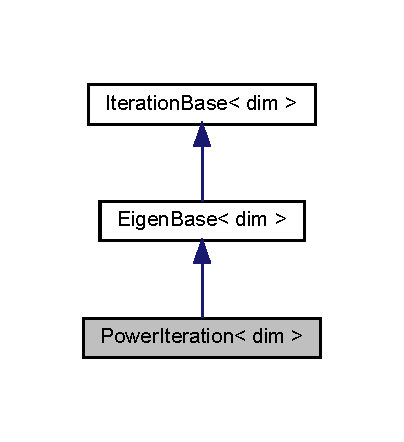
\includegraphics[width=194pt]{class_power_iteration__inherit__graph}
\end{center}
\end{figure}


Collaboration diagram for Power\+Iteration$<$ dim $>$\+:\nopagebreak
\begin{figure}[H]
\begin{center}
\leavevmode
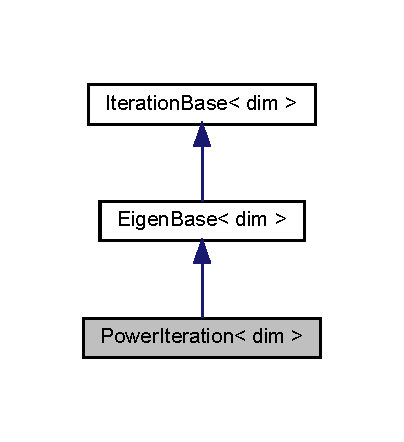
\includegraphics[width=194pt]{class_power_iteration__coll__graph}
\end{center}
\end{figure}
\subsection*{Public Member Functions}
\begin{DoxyCompactItemize}
\item 
\hyperlink{class_power_iteration_a2608445223ce7d27b24be0f9d7042554}{Power\+Iteration} (const Parameter\+Handler \&prm)
\item 
\hyperlink{class_power_iteration_ad660a351afc4f23b1bcf7b334ef033dd}{$\sim$\+Power\+Iteration} ()
\begin{DoxyCompactList}\small\item\em Class destructor. \end{DoxyCompactList}\item 
void \hyperlink{class_power_iteration_a583586002126f8b7a523e95327047cba}{eigen\+\_\+iterations} (std\+::vector$<$ Vector$<$ double $>$ $>$ \&sflxes\+\_\+proc, std\+::vector$<$ std\+\_\+cxx11\+::shared\+\_\+ptr$<$ \hyperlink{class_equation_base}{Equation\+Base}$<$ dim $>$ $>$ $>$ \&equ\+\_\+ptrs, std\+\_\+cxx11\+::shared\+\_\+ptr$<$ \hyperlink{class_i_g_base}{I\+G\+Base}$<$ dim $>$ $>$ ig\+\_\+ptr, std\+\_\+cxx11\+::shared\+\_\+ptr$<$ \hyperlink{class_m_g_base}{M\+G\+Base}$<$ dim $>$ $>$ mg\+\_\+ptr)
\end{DoxyCompactItemize}
\subsection*{Additional Inherited Members}


\subsection{Detailed Description}
\subsubsection*{template$<$int dim$>$\newline
class Power\+Iteration$<$ dim $>$}

This class provides power iteration scheme. 

This class implements power iteration for eigenvalue calculations. Assuming $T$, $S$ and $F$ are transport, scattering and fission operators, a power iteration scheme can be represented as \[ T\psi^{l+1}=S\psi^{l+1}+F\psi^l, \] where $l$ stands for eigenvalue iteration index.

\begin{DoxyAuthor}{Author}
Weixiong Zheng 
\end{DoxyAuthor}
\begin{DoxyDate}{Date}
2017/09 
\end{DoxyDate}


Definition at line 22 of file power\+\_\+iteration.\+h.



\subsection{Constructor \& Destructor Documentation}
\mbox{\Hypertarget{class_power_iteration_a2608445223ce7d27b24be0f9d7042554}\label{class_power_iteration_a2608445223ce7d27b24be0f9d7042554}} 
\index{Power\+Iteration@{Power\+Iteration}!Power\+Iteration@{Power\+Iteration}}
\index{Power\+Iteration@{Power\+Iteration}!Power\+Iteration@{Power\+Iteration}}
\subsubsection{\texorpdfstring{Power\+Iteration()}{PowerIteration()}}
{\footnotesize\ttfamily template$<$int dim$>$ \\
\hyperlink{class_power_iteration}{Power\+Iteration}$<$ dim $>$\+::\hyperlink{class_power_iteration}{Power\+Iteration} (\begin{DoxyParamCaption}\item[{const Parameter\+Handler \&}]{prm }\end{DoxyParamCaption})}

Class constructor.


\begin{DoxyParams}{Parameters}
{\em prm} & Parameter\+Handler object. \\
\hline
\end{DoxyParams}


Definition at line 4 of file power\+\_\+iteration.\+cc.

\mbox{\Hypertarget{class_power_iteration_ad660a351afc4f23b1bcf7b334ef033dd}\label{class_power_iteration_ad660a351afc4f23b1bcf7b334ef033dd}} 
\index{Power\+Iteration@{Power\+Iteration}!````~Power\+Iteration@{$\sim$\+Power\+Iteration}}
\index{````~Power\+Iteration@{$\sim$\+Power\+Iteration}!Power\+Iteration@{Power\+Iteration}}
\subsubsection{\texorpdfstring{$\sim$\+Power\+Iteration()}{~PowerIteration()}}
{\footnotesize\ttfamily template$<$int dim$>$ \\
\hyperlink{class_power_iteration}{Power\+Iteration}$<$ dim $>$\+::$\sim$\hyperlink{class_power_iteration}{Power\+Iteration} (\begin{DoxyParamCaption}{ }\end{DoxyParamCaption})}



Class destructor. 



Definition at line 11 of file power\+\_\+iteration.\+cc.



\subsection{Member Function Documentation}
\mbox{\Hypertarget{class_power_iteration_a583586002126f8b7a523e95327047cba}\label{class_power_iteration_a583586002126f8b7a523e95327047cba}} 
\index{Power\+Iteration@{Power\+Iteration}!eigen\+\_\+iterations@{eigen\+\_\+iterations}}
\index{eigen\+\_\+iterations@{eigen\+\_\+iterations}!Power\+Iteration@{Power\+Iteration}}
\subsubsection{\texorpdfstring{eigen\+\_\+iterations()}{eigen\_iterations()}}
{\footnotesize\ttfamily template$<$int dim$>$ \\
void \hyperlink{class_power_iteration}{Power\+Iteration}$<$ dim $>$\+::eigen\+\_\+iterations (\begin{DoxyParamCaption}\item[{std\+::vector$<$ Vector$<$ double $>$ $>$ \&}]{sflxes\+\_\+proc,  }\item[{std\+::vector$<$ std\+\_\+cxx11\+::shared\+\_\+ptr$<$ \hyperlink{class_equation_base}{Equation\+Base}$<$ dim $>$ $>$ $>$ \&}]{equ\+\_\+ptrs,  }\item[{std\+\_\+cxx11\+::shared\+\_\+ptr$<$ \hyperlink{class_i_g_base}{I\+G\+Base}$<$ dim $>$ $>$}]{ig\+\_\+ptr,  }\item[{std\+\_\+cxx11\+::shared\+\_\+ptr$<$ \hyperlink{class_m_g_base}{M\+G\+Base}$<$ dim $>$ $>$}]{mg\+\_\+ptr }\end{DoxyParamCaption})\hspace{0.3cm}{\ttfamily [virtual]}}

Eigenvalue iterations using power iteration scheme for eigenvalue calculations.


\begin{DoxyParams}{Parameters}
{\em sflxes\+\_\+proc} & Scalar fluxes for all groups living on current processor. \\
\hline
{\em equ\+\_\+ptrs} & Pointers of equations, i.\+e. Equation\+Base$<$dim$>$ objects. \\
\hline
{\em ig\+\_\+ptr} & Pointer of in-\/group solver, i.\+e. I\+G\+Base$<$dim$>$ object \\
\hline
{\em mg\+\_\+ptr} & Pointer of MG solver, i.\+e. M\+G\+Base$<$dim$>$ object. \\
\hline
\end{DoxyParams}
\begin{DoxyReturn}{Returns}
Void. 
\end{DoxyReturn}


Reimplemented from \hyperlink{class_eigen_base_ae09830ed4bcb14b7b699cd5f5460fab7}{Eigen\+Base$<$ dim $>$}.



Definition at line 17 of file power\+\_\+iteration.\+cc.



The documentation for this class was generated from the following files\+:\begin{DoxyCompactItemize}
\item 
src/iteration/\hyperlink{power__iteration_8h}{power\+\_\+iteration.\+h}\item 
src/iteration/\hyperlink{power__iteration_8cc}{power\+\_\+iteration.\+cc}\end{DoxyCompactItemize}

\hypertarget{class_preconditioner_solver}{}\section{Preconditioner\+Solver Class Reference}
\label{class_preconditioner_solver}\index{Preconditioner\+Solver@{Preconditioner\+Solver}}


The class provides linear solving functionalities.  




{\ttfamily \#include $<$preconditioner\+\_\+solver.\+h$>$}

\subsection*{Public Member Functions}
\begin{DoxyCompactItemize}
\item 
\hyperlink{class_preconditioner_solver_a5b49c94b10dc0e2b78ad278d19a8281d}{Preconditioner\+Solver} (const Parameter\+Handler \&prm, std\+::string \hyperlink{class_preconditioner_solver_af20758bf54111e7092c49688622b1e54}{equation\+\_\+name}, unsigned int \&\hyperlink{class_preconditioner_solver_ac2c59527a78b06037f0eb18132d8be63}{n\+\_\+total\+\_\+vars})
\item 
\hyperlink{class_preconditioner_solver_a8418873c20ded98dc1af3f66880d8e91}{$\sim$\+Preconditioner\+Solver} ()
\begin{DoxyCompactList}\small\item\em Class destructors. \end{DoxyCompactList}\item 
void \hyperlink{class_preconditioner_solver_adfb504161a00566d8adc3534d58b3611}{initialize\+\_\+preconditioners} (std\+::vector$<$ P\+E\+T\+Sc\+Wrappers\+::\+M\+P\+I\+::\+Sparse\+Matrix $\ast$$>$ \&sys\+\_\+mats, std\+::vector$<$ P\+E\+T\+Sc\+Wrappers\+::\+M\+P\+I\+::\+Vector $\ast$$>$ \&sys\+\_\+rhses)
\item 
void \hyperlink{class_preconditioner_solver_a5adc9e36ec12ed148eef7f1120c1bc4e}{linear\+\_\+algebra\+\_\+solve} (std\+::vector$<$ P\+E\+T\+Sc\+Wrappers\+::\+M\+P\+I\+::\+Sparse\+Matrix $\ast$$>$ \&sys\+\_\+mats, std\+::vector$<$ P\+E\+T\+Sc\+Wrappers\+::\+M\+P\+I\+::\+Vector $\ast$$>$ \&sys\+\_\+flxes, std\+::vector$<$ P\+E\+T\+Sc\+Wrappers\+::\+M\+P\+I\+::\+Vector $\ast$$>$ \&sys\+\_\+rhses, unsigned int \&i)
\end{DoxyCompactItemize}
\subsection*{Private Attributes}
\begin{DoxyCompactItemize}
\item 
const unsigned int \hyperlink{class_preconditioner_solver_ac2c59527a78b06037f0eb18132d8be63}{n\+\_\+total\+\_\+vars}
\begin{DoxyCompactList}\small\item\em Total number of variables in the target system. \end{DoxyCompactList}\item 
const std\+::string \hyperlink{class_preconditioner_solver_af20758bf54111e7092c49688622b1e54}{equation\+\_\+name}
\begin{DoxyCompactList}\small\item\em Name of the target equation. \end{DoxyCompactList}\item 
bool \hyperlink{class_preconditioner_solver_a954ef4f8c7d8206b277280a4b41aa9b1}{have\+\_\+reflective\+\_\+bc}
\begin{DoxyCompactList}\small\item\em Booolean to determine if there\textquotesingle{}s any reflective boundary. \end{DoxyCompactList}\item 
double \hyperlink{class_preconditioner_solver_ab9548e7699e82a2b006db283c59e4a80}{ssor\+\_\+omega}
\begin{DoxyCompactList}\small\item\em The relaxation factor if block S\+S\+OR is used as preconditioner. \end{DoxyCompactList}\item 
std\+::string \hyperlink{class_preconditioner_solver_ae13f7d32f80aad8eb1a4a9d1d2c4d019}{linear\+\_\+solver\+\_\+name}
\begin{DoxyCompactList}\small\item\em Linear solver name for current equation. \end{DoxyCompactList}\item 
std\+::string \hyperlink{class_preconditioner_solver_a2d8afd11d073e87487da0442486c3e48}{preconditioner\+\_\+name}
\begin{DoxyCompactList}\small\item\em Preconditioner name for current equation. \end{DoxyCompactList}\item 
std\+::vector$<$ bool $>$ \hyperlink{class_preconditioner_solver_a0241f0b26a8c964fc1e3fd8fef5a20a6}{direct\+\_\+init}
\begin{DoxyCompactList}\small\item\em A vector of boolean to determine if direct solver of a component is initilized. \end{DoxyCompactList}\item 
std\+::vector$<$ unsigned int $>$ \hyperlink{class_preconditioner_solver_a09b25f234ad6a225fb8a002fc919181a}{linear\+\_\+iters}
\begin{DoxyCompactList}\small\item\em A vector of integers showing number of iterations in linear solves. \end{DoxyCompactList}\item 
std\+\_\+cxx11\+::shared\+\_\+ptr$<$ Solver\+Control $>$ \hyperlink{class_preconditioner_solver_a3170128a1c287f729fa40c9aff2f2eed}{cn}
\begin{DoxyCompactList}\small\item\em pointer of \href{https://www.dealii.org/8.4.1/doxygen/deal.II/classSolverControl.html}{\tt {\bfseries Solver\+Control}} object. \end{DoxyCompactList}\item 
std\+::vector$<$ std\+\_\+cxx11\+::shared\+\_\+ptr$<$ P\+E\+T\+Sc\+Wrappers\+::\+Precondition\+Boomer\+A\+MG $>$ $>$ \hyperlink{class_preconditioner_solver_a235b12fcd8e5978c1a3df8c76d05808b}{pre\+\_\+amg}
\begin{DoxyCompactList}\small\item\em A vector of pointers of \href{https://www.dealii.org/8.5.0/doxygen/deal.II/classPETScWrappers_1_1PreconditionBoomerAMG.html}{\tt {\bfseries Boomer\+A\+MG}} preconditioner. \end{DoxyCompactList}\item 
std\+::vector$<$ std\+\_\+cxx11\+::shared\+\_\+ptr$<$ P\+E\+T\+Sc\+Wrappers\+::\+Precondition\+Block\+Jacobi $>$ $>$ \hyperlink{class_preconditioner_solver_af3d0217e39b9527c67ac6ce56464f11a}{pre\+\_\+bjacobi}
\begin{DoxyCompactList}\small\item\em A vector of pointers of \href{https://www.dealii.org/8.5.0/doxygen/deal.II/classPETScWrappers_1_1PreconditionBlockJacobi.html}{\tt {\bfseries block Jacobi}} preconditioner. \end{DoxyCompactList}\item 
std\+::vector$<$ std\+\_\+cxx11\+::shared\+\_\+ptr$<$ P\+E\+T\+Sc\+Wrappers\+::\+Precondition\+Para\+Sails $>$ $>$ \hyperlink{class_preconditioner_solver_a90b15442f60786b56729f2756e191336}{pre\+\_\+parasails}
\begin{DoxyCompactList}\small\item\em A vector of pointers of \href{https://www.dealii.org/8.5.0/doxygen/deal.II/classPETScWrappers_1_1PreconditionParaSails.html}{\tt {\bfseries Para\+Sails}} preconditioner. \end{DoxyCompactList}\item 
std\+::vector$<$ std\+\_\+cxx11\+::shared\+\_\+ptr$<$ P\+E\+T\+Sc\+Wrappers\+::\+Precondition\+Jacobi $>$ $>$ \hyperlink{class_preconditioner_solver_ab2379323cfbca020045ec5dd4ab708dc}{pre\+\_\+jacobi}
\begin{DoxyCompactList}\small\item\em A vector of pointers of \href{https://www.dealii.org/8.5.0/doxygen/deal.II/classPETScWrappers_1_1PreconditionJacobi.html}{\tt {\bfseries Jacobi}} preconditioner. \end{DoxyCompactList}\item 
std\+::vector$<$ std\+\_\+cxx11\+::shared\+\_\+ptr$<$ P\+E\+T\+Sc\+Wrappers\+::\+Precondition\+Eisenstat $>$ $>$ \hyperlink{class_preconditioner_solver_aab4bd157aebca7681283ff6cf0e69392}{pre\+\_\+eisenstat}
\begin{DoxyCompactList}\small\item\em A vector of pointers of \href{https://www.dealii.org/8.5.0/doxygen/deal.II/classPETScWrappers_1_1PreconditionEisenstat.html}{\tt {\bfseries Eisenstat}} (block S\+S\+OR) preconditioner. \end{DoxyCompactList}\item 
std\+::vector$<$ std\+\_\+cxx11\+::shared\+\_\+ptr$<$ P\+E\+T\+Sc\+Wrappers\+::\+Sparse\+Direct\+M\+U\+M\+PS $>$ $>$ \hyperlink{class_preconditioner_solver_acd3bde261fb29c50e15ffe6ecd78ee5f}{direct}
\begin{DoxyCompactList}\small\item\em A vector of pointers of \href{https://www.dealii.org/8.5.0/doxygen/deal.II/classPETScWrappers_1_1SparseDirectMUMPS.html}{\tt {\bfseries M\+U\+M\+PS}} solver objects. \end{DoxyCompactList}\end{DoxyCompactItemize}


\subsection{Detailed Description}
The class provides linear solving functionalities. 

This class is a wrapper class aiming to simplifies linear solving process. deal.\+II algebraic preconditioner wrappers and solver wrappers will be called to utilize P\+E\+T\+Sc linear solving functionalities in parallel. This class only provide two functions interfaces outside\+: initialize\+\_\+preconditioners and linear\+\_\+algebraic\+\_\+solve.

About how to use this class\+:

(1) Everytime a new equation is assembled, call initialize\+\_\+preconditioners to either initilize preconditioners if iterative solvers are used or initilize factorization for direct solver based on M\+U\+M\+PS. Note that initialization only needs to be done once per equation.

(2) Call linear\+\_\+algebra\+\_\+solve whenever needed.

For details of P\+E\+T\+Sc wrappers of linear algebra functions/objects, refer to \href{https://www.dealii.org/8.5.0/doxygen/deal.II/group__PETScWrappers.html}{\tt {\bfseries P\+E\+T\+Sc\+Wrappers}}.

\begin{DoxyAuthor}{Author}
Weixiong Zheng 
\end{DoxyAuthor}
\begin{DoxyDate}{Date}
2017/10 
\end{DoxyDate}


Definition at line 38 of file preconditioner\+\_\+solver.\+h.



\subsection{Constructor \& Destructor Documentation}
\mbox{\Hypertarget{class_preconditioner_solver_a5b49c94b10dc0e2b78ad278d19a8281d}\label{class_preconditioner_solver_a5b49c94b10dc0e2b78ad278d19a8281d}} 
\index{Preconditioner\+Solver@{Preconditioner\+Solver}!Preconditioner\+Solver@{Preconditioner\+Solver}}
\index{Preconditioner\+Solver@{Preconditioner\+Solver}!Preconditioner\+Solver@{Preconditioner\+Solver}}
\subsubsection{\texorpdfstring{Preconditioner\+Solver()}{PreconditionerSolver()}}
{\footnotesize\ttfamily Preconditioner\+Solver\+::\+Preconditioner\+Solver (\begin{DoxyParamCaption}\item[{const Parameter\+Handler \&}]{prm,  }\item[{std\+::string}]{equation\+\_\+name,  }\item[{unsigned int \&}]{n\+\_\+total\+\_\+vars }\end{DoxyParamCaption})}

Class constructor.


\begin{DoxyParams}{Parameters}
{\em prm} & A Parameter\+Handler object containing all user defined parameters. \\
\hline
{\em equation\+\_\+name} & A string describing the name of the target equation. \\
\hline
{\em n\+\_\+total\+\_\+vars} & A integer for the total number components for target equation. \\
\hline
\end{DoxyParams}


Definition at line 3 of file preconditioner\+\_\+solver.\+cc.

\mbox{\Hypertarget{class_preconditioner_solver_a8418873c20ded98dc1af3f66880d8e91}\label{class_preconditioner_solver_a8418873c20ded98dc1af3f66880d8e91}} 
\index{Preconditioner\+Solver@{Preconditioner\+Solver}!````~Preconditioner\+Solver@{$\sim$\+Preconditioner\+Solver}}
\index{````~Preconditioner\+Solver@{$\sim$\+Preconditioner\+Solver}!Preconditioner\+Solver@{Preconditioner\+Solver}}
\subsubsection{\texorpdfstring{$\sim$\+Preconditioner\+Solver()}{~PreconditionerSolver()}}
{\footnotesize\ttfamily Preconditioner\+Solver\+::$\sim$\+Preconditioner\+Solver (\begin{DoxyParamCaption}{ }\end{DoxyParamCaption})}



Class destructors. 



Definition at line 35 of file preconditioner\+\_\+solver.\+cc.



\subsection{Member Function Documentation}
\mbox{\Hypertarget{class_preconditioner_solver_adfb504161a00566d8adc3534d58b3611}\label{class_preconditioner_solver_adfb504161a00566d8adc3534d58b3611}} 
\index{Preconditioner\+Solver@{Preconditioner\+Solver}!initialize\+\_\+preconditioners@{initialize\+\_\+preconditioners}}
\index{initialize\+\_\+preconditioners@{initialize\+\_\+preconditioners}!Preconditioner\+Solver@{Preconditioner\+Solver}}
\subsubsection{\texorpdfstring{initialize\+\_\+preconditioners()}{initialize\_preconditioners()}}
{\footnotesize\ttfamily void Preconditioner\+Solver\+::initialize\+\_\+preconditioners (\begin{DoxyParamCaption}\item[{std\+::vector$<$ P\+E\+T\+Sc\+Wrappers\+::\+M\+P\+I\+::\+Sparse\+Matrix $\ast$$>$ \&}]{sys\+\_\+mats,  }\item[{std\+::vector$<$ P\+E\+T\+Sc\+Wrappers\+::\+M\+P\+I\+::\+Vector $\ast$$>$ \&}]{sys\+\_\+rhses }\end{DoxyParamCaption})}

This function initilizes preconditioners for an equation. The main functionalities include one of the following two points\+:

(1) For iterative solvers, initializing preconditioners and store them in shared\+\_\+ptr\textquotesingle{}s.

(2) For M\+U\+M\+PS direct solver, initializing factorizations and store them in shared\+\_\+ptr\textquotesingle{}s.


\begin{DoxyParams}{Parameters}
{\em sys\+\_\+mats} & A vector of pointers to system matrices of the target equation. \\
\hline
{\em sys\+\_\+rhses} & A vector of pointers to system right-\/hand-\/side vectors of the target equation. \\
\hline
\end{DoxyParams}


Definition at line 41 of file preconditioner\+\_\+solver.\+cc.

\mbox{\Hypertarget{class_preconditioner_solver_a5adc9e36ec12ed148eef7f1120c1bc4e}\label{class_preconditioner_solver_a5adc9e36ec12ed148eef7f1120c1bc4e}} 
\index{Preconditioner\+Solver@{Preconditioner\+Solver}!linear\+\_\+algebra\+\_\+solve@{linear\+\_\+algebra\+\_\+solve}}
\index{linear\+\_\+algebra\+\_\+solve@{linear\+\_\+algebra\+\_\+solve}!Preconditioner\+Solver@{Preconditioner\+Solver}}
\subsubsection{\texorpdfstring{linear\+\_\+algebra\+\_\+solve()}{linear\_algebra\_solve()}}
{\footnotesize\ttfamily void Preconditioner\+Solver\+::linear\+\_\+algebra\+\_\+solve (\begin{DoxyParamCaption}\item[{std\+::vector$<$ P\+E\+T\+Sc\+Wrappers\+::\+M\+P\+I\+::\+Sparse\+Matrix $\ast$$>$ \&}]{sys\+\_\+mats,  }\item[{std\+::vector$<$ P\+E\+T\+Sc\+Wrappers\+::\+M\+P\+I\+::\+Vector $\ast$$>$ \&}]{sys\+\_\+flxes,  }\item[{std\+::vector$<$ P\+E\+T\+Sc\+Wrappers\+::\+M\+P\+I\+::\+Vector $\ast$$>$ \&}]{sys\+\_\+rhses,  }\item[{unsigned int \&}]{i }\end{DoxyParamCaption})}

This function provide functionality of performing linear algebraic solve for a specific component of the target equation.


\begin{DoxyParams}{Parameters}
{\em sys\+\_\+mats} & A vector of pointers to system matrices of the target equation. \\
\hline
{\em sys\+\_\+flxes} & A vector of pointers to system solutions of the target equation \\
\hline
{\em sys\+\_\+rhses} & A vector of pointers to system right-\/hand-\/side vectors of the target equation. \\
\hline
{\em i} & An integer specifying the component index of interest. \\
\hline
\end{DoxyParams}
\begin{DoxyReturn}{Returns}
Void. 
\end{DoxyReturn}


Definition at line 129 of file preconditioner\+\_\+solver.\+cc.



\subsection{Member Data Documentation}
\mbox{\Hypertarget{class_preconditioner_solver_a3170128a1c287f729fa40c9aff2f2eed}\label{class_preconditioner_solver_a3170128a1c287f729fa40c9aff2f2eed}} 
\index{Preconditioner\+Solver@{Preconditioner\+Solver}!cn@{cn}}
\index{cn@{cn}!Preconditioner\+Solver@{Preconditioner\+Solver}}
\subsubsection{\texorpdfstring{cn}{cn}}
{\footnotesize\ttfamily std\+\_\+cxx11\+::shared\+\_\+ptr$<$Solver\+Control$>$ Preconditioner\+Solver\+::cn\hspace{0.3cm}{\ttfamily [private]}}



pointer of \href{https://www.dealii.org/8.4.1/doxygen/deal.II/classSolverControl.html}{\tt {\bfseries Solver\+Control}} object. 

Control iterative algebraic linear solvers to determine convergence. Can be used to show number of linear iterations in the algebraic solve, linear solver residual after each iteration etc. 

Definition at line 112 of file preconditioner\+\_\+solver.\+h.

\mbox{\Hypertarget{class_preconditioner_solver_acd3bde261fb29c50e15ffe6ecd78ee5f}\label{class_preconditioner_solver_acd3bde261fb29c50e15ffe6ecd78ee5f}} 
\index{Preconditioner\+Solver@{Preconditioner\+Solver}!direct@{direct}}
\index{direct@{direct}!Preconditioner\+Solver@{Preconditioner\+Solver}}
\subsubsection{\texorpdfstring{direct}{direct}}
{\footnotesize\ttfamily std\+::vector$<$std\+\_\+cxx11\+::shared\+\_\+ptr$<$P\+E\+T\+Sc\+Wrappers\+::\+Sparse\+Direct\+M\+U\+M\+PS$>$ $>$ Preconditioner\+Solver\+::direct\hspace{0.3cm}{\ttfamily [private]}}



A vector of pointers of \href{https://www.dealii.org/8.5.0/doxygen/deal.II/classPETScWrappers_1_1SparseDirectMUMPS.html}{\tt {\bfseries M\+U\+M\+PS}} solver objects. 



Definition at line 130 of file preconditioner\+\_\+solver.\+h.

\mbox{\Hypertarget{class_preconditioner_solver_a0241f0b26a8c964fc1e3fd8fef5a20a6}\label{class_preconditioner_solver_a0241f0b26a8c964fc1e3fd8fef5a20a6}} 
\index{Preconditioner\+Solver@{Preconditioner\+Solver}!direct\+\_\+init@{direct\+\_\+init}}
\index{direct\+\_\+init@{direct\+\_\+init}!Preconditioner\+Solver@{Preconditioner\+Solver}}
\subsubsection{\texorpdfstring{direct\+\_\+init}{direct\_init}}
{\footnotesize\ttfamily std\+::vector$<$bool$>$ Preconditioner\+Solver\+::direct\+\_\+init\hspace{0.3cm}{\ttfamily [private]}}



A vector of boolean to determine if direct solver of a component is initilized. 



Definition at line 101 of file preconditioner\+\_\+solver.\+h.

\mbox{\Hypertarget{class_preconditioner_solver_af20758bf54111e7092c49688622b1e54}\label{class_preconditioner_solver_af20758bf54111e7092c49688622b1e54}} 
\index{Preconditioner\+Solver@{Preconditioner\+Solver}!equation\+\_\+name@{equation\+\_\+name}}
\index{equation\+\_\+name@{equation\+\_\+name}!Preconditioner\+Solver@{Preconditioner\+Solver}}
\subsubsection{\texorpdfstring{equation\+\_\+name}{equation\_name}}
{\footnotesize\ttfamily const std\+::string Preconditioner\+Solver\+::equation\+\_\+name\hspace{0.3cm}{\ttfamily [private]}}



Name of the target equation. 



Definition at line 92 of file preconditioner\+\_\+solver.\+h.

\mbox{\Hypertarget{class_preconditioner_solver_a954ef4f8c7d8206b277280a4b41aa9b1}\label{class_preconditioner_solver_a954ef4f8c7d8206b277280a4b41aa9b1}} 
\index{Preconditioner\+Solver@{Preconditioner\+Solver}!have\+\_\+reflective\+\_\+bc@{have\+\_\+reflective\+\_\+bc}}
\index{have\+\_\+reflective\+\_\+bc@{have\+\_\+reflective\+\_\+bc}!Preconditioner\+Solver@{Preconditioner\+Solver}}
\subsubsection{\texorpdfstring{have\+\_\+reflective\+\_\+bc}{have\_reflective\_bc}}
{\footnotesize\ttfamily bool Preconditioner\+Solver\+::have\+\_\+reflective\+\_\+bc\hspace{0.3cm}{\ttfamily [private]}}



Booolean to determine if there\textquotesingle{}s any reflective boundary. 



Definition at line 94 of file preconditioner\+\_\+solver.\+h.

\mbox{\Hypertarget{class_preconditioner_solver_a09b25f234ad6a225fb8a002fc919181a}\label{class_preconditioner_solver_a09b25f234ad6a225fb8a002fc919181a}} 
\index{Preconditioner\+Solver@{Preconditioner\+Solver}!linear\+\_\+iters@{linear\+\_\+iters}}
\index{linear\+\_\+iters@{linear\+\_\+iters}!Preconditioner\+Solver@{Preconditioner\+Solver}}
\subsubsection{\texorpdfstring{linear\+\_\+iters}{linear\_iters}}
{\footnotesize\ttfamily std\+::vector$<$unsigned int$>$ Preconditioner\+Solver\+::linear\+\_\+iters\hspace{0.3cm}{\ttfamily [private]}}



A vector of integers showing number of iterations in linear solves. 



Definition at line 104 of file preconditioner\+\_\+solver.\+h.

\mbox{\Hypertarget{class_preconditioner_solver_ae13f7d32f80aad8eb1a4a9d1d2c4d019}\label{class_preconditioner_solver_ae13f7d32f80aad8eb1a4a9d1d2c4d019}} 
\index{Preconditioner\+Solver@{Preconditioner\+Solver}!linear\+\_\+solver\+\_\+name@{linear\+\_\+solver\+\_\+name}}
\index{linear\+\_\+solver\+\_\+name@{linear\+\_\+solver\+\_\+name}!Preconditioner\+Solver@{Preconditioner\+Solver}}
\subsubsection{\texorpdfstring{linear\+\_\+solver\+\_\+name}{linear\_solver\_name}}
{\footnotesize\ttfamily std\+::string Preconditioner\+Solver\+::linear\+\_\+solver\+\_\+name\hspace{0.3cm}{\ttfamily [private]}}



Linear solver name for current equation. 



Definition at line 97 of file preconditioner\+\_\+solver.\+h.

\mbox{\Hypertarget{class_preconditioner_solver_ac2c59527a78b06037f0eb18132d8be63}\label{class_preconditioner_solver_ac2c59527a78b06037f0eb18132d8be63}} 
\index{Preconditioner\+Solver@{Preconditioner\+Solver}!n\+\_\+total\+\_\+vars@{n\+\_\+total\+\_\+vars}}
\index{n\+\_\+total\+\_\+vars@{n\+\_\+total\+\_\+vars}!Preconditioner\+Solver@{Preconditioner\+Solver}}
\subsubsection{\texorpdfstring{n\+\_\+total\+\_\+vars}{n\_total\_vars}}
{\footnotesize\ttfamily const unsigned int Preconditioner\+Solver\+::n\+\_\+total\+\_\+vars\hspace{0.3cm}{\ttfamily [private]}}



Total number of variables in the target system. 



Definition at line 91 of file preconditioner\+\_\+solver.\+h.

\mbox{\Hypertarget{class_preconditioner_solver_a235b12fcd8e5978c1a3df8c76d05808b}\label{class_preconditioner_solver_a235b12fcd8e5978c1a3df8c76d05808b}} 
\index{Preconditioner\+Solver@{Preconditioner\+Solver}!pre\+\_\+amg@{pre\+\_\+amg}}
\index{pre\+\_\+amg@{pre\+\_\+amg}!Preconditioner\+Solver@{Preconditioner\+Solver}}
\subsubsection{\texorpdfstring{pre\+\_\+amg}{pre\_amg}}
{\footnotesize\ttfamily std\+::vector$<$std\+\_\+cxx11\+::shared\+\_\+ptr$<$P\+E\+T\+Sc\+Wrappers\+::\+Precondition\+Boomer\+A\+MG$>$ $>$ Preconditioner\+Solver\+::pre\+\_\+amg\hspace{0.3cm}{\ttfamily [private]}}



A vector of pointers of \href{https://www.dealii.org/8.5.0/doxygen/deal.II/classPETScWrappers_1_1PreconditionBoomerAMG.html}{\tt {\bfseries Boomer\+A\+MG}} preconditioner. 



Definition at line 115 of file preconditioner\+\_\+solver.\+h.

\mbox{\Hypertarget{class_preconditioner_solver_af3d0217e39b9527c67ac6ce56464f11a}\label{class_preconditioner_solver_af3d0217e39b9527c67ac6ce56464f11a}} 
\index{Preconditioner\+Solver@{Preconditioner\+Solver}!pre\+\_\+bjacobi@{pre\+\_\+bjacobi}}
\index{pre\+\_\+bjacobi@{pre\+\_\+bjacobi}!Preconditioner\+Solver@{Preconditioner\+Solver}}
\subsubsection{\texorpdfstring{pre\+\_\+bjacobi}{pre\_bjacobi}}
{\footnotesize\ttfamily std\+::vector$<$std\+\_\+cxx11\+::shared\+\_\+ptr$<$P\+E\+T\+Sc\+Wrappers\+::\+Precondition\+Block\+Jacobi$>$ $>$ Preconditioner\+Solver\+::pre\+\_\+bjacobi\hspace{0.3cm}{\ttfamily [private]}}



A vector of pointers of \href{https://www.dealii.org/8.5.0/doxygen/deal.II/classPETScWrappers_1_1PreconditionBlockJacobi.html}{\tt {\bfseries block Jacobi}} preconditioner. 



Definition at line 118 of file preconditioner\+\_\+solver.\+h.

\mbox{\Hypertarget{class_preconditioner_solver_aab4bd157aebca7681283ff6cf0e69392}\label{class_preconditioner_solver_aab4bd157aebca7681283ff6cf0e69392}} 
\index{Preconditioner\+Solver@{Preconditioner\+Solver}!pre\+\_\+eisenstat@{pre\+\_\+eisenstat}}
\index{pre\+\_\+eisenstat@{pre\+\_\+eisenstat}!Preconditioner\+Solver@{Preconditioner\+Solver}}
\subsubsection{\texorpdfstring{pre\+\_\+eisenstat}{pre\_eisenstat}}
{\footnotesize\ttfamily std\+::vector$<$std\+\_\+cxx11\+::shared\+\_\+ptr$<$P\+E\+T\+Sc\+Wrappers\+::\+Precondition\+Eisenstat$>$ $>$ Preconditioner\+Solver\+::pre\+\_\+eisenstat\hspace{0.3cm}{\ttfamily [private]}}



A vector of pointers of \href{https://www.dealii.org/8.5.0/doxygen/deal.II/classPETScWrappers_1_1PreconditionEisenstat.html}{\tt {\bfseries Eisenstat}} (block S\+S\+OR) preconditioner. 



Definition at line 127 of file preconditioner\+\_\+solver.\+h.

\mbox{\Hypertarget{class_preconditioner_solver_ab2379323cfbca020045ec5dd4ab708dc}\label{class_preconditioner_solver_ab2379323cfbca020045ec5dd4ab708dc}} 
\index{Preconditioner\+Solver@{Preconditioner\+Solver}!pre\+\_\+jacobi@{pre\+\_\+jacobi}}
\index{pre\+\_\+jacobi@{pre\+\_\+jacobi}!Preconditioner\+Solver@{Preconditioner\+Solver}}
\subsubsection{\texorpdfstring{pre\+\_\+jacobi}{pre\_jacobi}}
{\footnotesize\ttfamily std\+::vector$<$std\+\_\+cxx11\+::shared\+\_\+ptr$<$P\+E\+T\+Sc\+Wrappers\+::\+Precondition\+Jacobi$>$ $>$ Preconditioner\+Solver\+::pre\+\_\+jacobi\hspace{0.3cm}{\ttfamily [private]}}



A vector of pointers of \href{https://www.dealii.org/8.5.0/doxygen/deal.II/classPETScWrappers_1_1PreconditionJacobi.html}{\tt {\bfseries Jacobi}} preconditioner. 



Definition at line 124 of file preconditioner\+\_\+solver.\+h.

\mbox{\Hypertarget{class_preconditioner_solver_a90b15442f60786b56729f2756e191336}\label{class_preconditioner_solver_a90b15442f60786b56729f2756e191336}} 
\index{Preconditioner\+Solver@{Preconditioner\+Solver}!pre\+\_\+parasails@{pre\+\_\+parasails}}
\index{pre\+\_\+parasails@{pre\+\_\+parasails}!Preconditioner\+Solver@{Preconditioner\+Solver}}
\subsubsection{\texorpdfstring{pre\+\_\+parasails}{pre\_parasails}}
{\footnotesize\ttfamily std\+::vector$<$std\+\_\+cxx11\+::shared\+\_\+ptr$<$P\+E\+T\+Sc\+Wrappers\+::\+Precondition\+Para\+Sails$>$ $>$ Preconditioner\+Solver\+::pre\+\_\+parasails\hspace{0.3cm}{\ttfamily [private]}}



A vector of pointers of \href{https://www.dealii.org/8.5.0/doxygen/deal.II/classPETScWrappers_1_1PreconditionParaSails.html}{\tt {\bfseries Para\+Sails}} preconditioner. 



Definition at line 121 of file preconditioner\+\_\+solver.\+h.

\mbox{\Hypertarget{class_preconditioner_solver_a2d8afd11d073e87487da0442486c3e48}\label{class_preconditioner_solver_a2d8afd11d073e87487da0442486c3e48}} 
\index{Preconditioner\+Solver@{Preconditioner\+Solver}!preconditioner\+\_\+name@{preconditioner\+\_\+name}}
\index{preconditioner\+\_\+name@{preconditioner\+\_\+name}!Preconditioner\+Solver@{Preconditioner\+Solver}}
\subsubsection{\texorpdfstring{preconditioner\+\_\+name}{preconditioner\_name}}
{\footnotesize\ttfamily std\+::string Preconditioner\+Solver\+::preconditioner\+\_\+name\hspace{0.3cm}{\ttfamily [private]}}



Preconditioner name for current equation. 



Definition at line 98 of file preconditioner\+\_\+solver.\+h.

\mbox{\Hypertarget{class_preconditioner_solver_ab9548e7699e82a2b006db283c59e4a80}\label{class_preconditioner_solver_ab9548e7699e82a2b006db283c59e4a80}} 
\index{Preconditioner\+Solver@{Preconditioner\+Solver}!ssor\+\_\+omega@{ssor\+\_\+omega}}
\index{ssor\+\_\+omega@{ssor\+\_\+omega}!Preconditioner\+Solver@{Preconditioner\+Solver}}
\subsubsection{\texorpdfstring{ssor\+\_\+omega}{ssor\_omega}}
{\footnotesize\ttfamily double Preconditioner\+Solver\+::ssor\+\_\+omega\hspace{0.3cm}{\ttfamily [private]}}



The relaxation factor if block S\+S\+OR is used as preconditioner. 



Definition at line 95 of file preconditioner\+\_\+solver.\+h.



The documentation for this class was generated from the following files\+:\begin{DoxyCompactItemize}
\item 
src/common/\hyperlink{preconditioner__solver_8h}{preconditioner\+\_\+solver.\+h}\item 
src/common/\hyperlink{preconditioner__solver_8cc}{preconditioner\+\_\+solver.\+cc}\end{DoxyCompactItemize}

\hypertarget{class_problem_definition}{}\section{Problem\+Definition Class Reference}
\label{class_problem_definition}\index{Problem\+Definition@{Problem\+Definition}}


This class performs parameter parsing.  




{\ttfamily \#include $<$problem\+\_\+definition.\+h$>$}

\subsection*{Public Member Functions}
\begin{DoxyCompactItemize}
\item 
\hyperlink{class_problem_definition_ad5d05724dd7de8e362f0c8db129744f9}{Problem\+Definition} ()
\begin{DoxyCompactList}\small\item\em Class constructor. \end{DoxyCompactList}\item 
\hyperlink{class_problem_definition_a6aa61be43188cf28040bd0e7d2bf02e3}{$\sim$\+Problem\+Definition} ()
\begin{DoxyCompactList}\small\item\em Class destructor. \end{DoxyCompactList}\end{DoxyCompactItemize}
\subsection*{Static Public Member Functions}
\begin{DoxyCompactItemize}
\item 
static void \hyperlink{class_problem_definition_a0a68b3c08b69729642dcfd37f23e7494}{declare\+\_\+parameters} (Parameter\+Handler \&prm)
\end{DoxyCompactItemize}


\subsection{Detailed Description}
This class performs parameter parsing. 

This class handles user-\/defined parameters. For details about parameter parsing, refer to \href{https://www.dealii.org/8.5.0/doxygen/deal.II/classParameterHa
ndler.html}{\tt {\bfseries Parameter\+Handler}}.

\begin{DoxyAuthor}{Author}
Weixiong Zheng 
\end{DoxyAuthor}
\begin{DoxyDate}{Date}
2017/06 
\end{DoxyDate}


Definition at line 31 of file problem\+\_\+definition.\+h.



\subsection{Constructor \& Destructor Documentation}
\mbox{\Hypertarget{class_problem_definition_ad5d05724dd7de8e362f0c8db129744f9}\label{class_problem_definition_ad5d05724dd7de8e362f0c8db129744f9}} 
\index{Problem\+Definition@{Problem\+Definition}!Problem\+Definition@{Problem\+Definition}}
\index{Problem\+Definition@{Problem\+Definition}!Problem\+Definition@{Problem\+Definition}}
\subsubsection{\texorpdfstring{Problem\+Definition()}{ProblemDefinition()}}
{\footnotesize\ttfamily Problem\+Definition\+::\+Problem\+Definition (\begin{DoxyParamCaption}{ }\end{DoxyParamCaption})}



Class constructor. 



Definition at line 11 of file problem\+\_\+definition.\+cc.

\mbox{\Hypertarget{class_problem_definition_a6aa61be43188cf28040bd0e7d2bf02e3}\label{class_problem_definition_a6aa61be43188cf28040bd0e7d2bf02e3}} 
\index{Problem\+Definition@{Problem\+Definition}!````~Problem\+Definition@{$\sim$\+Problem\+Definition}}
\index{````~Problem\+Definition@{$\sim$\+Problem\+Definition}!Problem\+Definition@{Problem\+Definition}}
\subsubsection{\texorpdfstring{$\sim$\+Problem\+Definition()}{~ProblemDefinition()}}
{\footnotesize\ttfamily Problem\+Definition\+::$\sim$\+Problem\+Definition (\begin{DoxyParamCaption}{ }\end{DoxyParamCaption})}



Class destructor. 



Definition at line 15 of file problem\+\_\+definition.\+cc.



\subsection{Member Function Documentation}
\mbox{\Hypertarget{class_problem_definition_a0a68b3c08b69729642dcfd37f23e7494}\label{class_problem_definition_a0a68b3c08b69729642dcfd37f23e7494}} 
\index{Problem\+Definition@{Problem\+Definition}!declare\+\_\+parameters@{declare\+\_\+parameters}}
\index{declare\+\_\+parameters@{declare\+\_\+parameters}!Problem\+Definition@{Problem\+Definition}}
\subsubsection{\texorpdfstring{declare\+\_\+parameters()}{declare\_parameters()}}
{\footnotesize\ttfamily void Problem\+Definition\+::declare\+\_\+parameters (\begin{DoxyParamCaption}\item[{Parameter\+Handler \&}]{prm }\end{DoxyParamCaption})\hspace{0.3cm}{\ttfamily [static]}}

This function process Parameter\+Handler object using info read from user-\/provided input. Specifically, it declares all possible parameter entries and parse info from user-\/defined input file to prm. After the processing, prm contains all the necessary info to define the problem and ready for other classes to retrieve the info.


\begin{DoxyParams}{Parameters}
{\em prm} & Parameter\+Handler object. \\
\hline
\end{DoxyParams}
\begin{DoxyReturn}{Returns}
Void. 
\end{DoxyReturn}


Definition at line 19 of file problem\+\_\+definition.\+cc.

Here is the caller graph for this function\+:\nopagebreak
\begin{figure}[H]
\begin{center}
\leavevmode
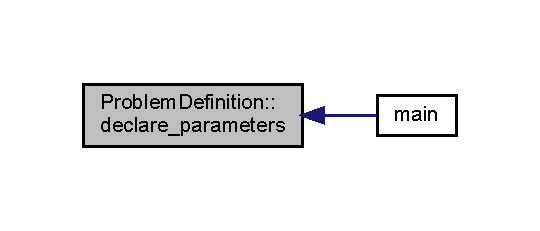
\includegraphics[width=259pt]{class_problem_definition_a0a68b3c08b69729642dcfd37f23e7494_icgraph}
\end{center}
\end{figure}


The documentation for this class was generated from the following files\+:\begin{DoxyCompactItemize}
\item 
src/common/\hyperlink{problem__definition_8h}{problem\+\_\+definition.\+h}\item 
src/common/\hyperlink{problem__definition_8cc}{problem\+\_\+definition.\+cc}\end{DoxyCompactItemize}

\hypertarget{class_source_iteration}{}\section{Source\+Iteration$<$ dim $>$ Class Template Reference}
\label{class_source_iteration}\index{Source\+Iteration$<$ dim $>$@{Source\+Iteration$<$ dim $>$}}


This class provides source iteration scheme for in group solve.  




{\ttfamily \#include $<$ig\+\_\+base.\+h$>$}



Inheritance diagram for Source\+Iteration$<$ dim $>$\+:\nopagebreak
\begin{figure}[H]
\begin{center}
\leavevmode
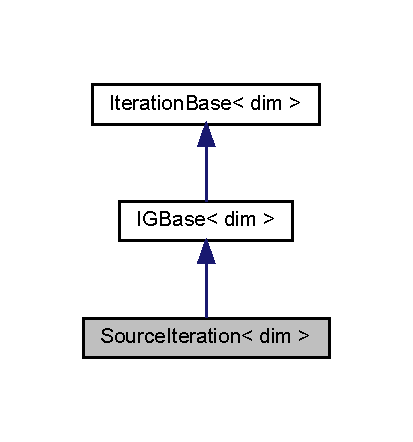
\includegraphics[width=198pt]{class_source_iteration__inherit__graph}
\end{center}
\end{figure}


Collaboration diagram for Source\+Iteration$<$ dim $>$\+:\nopagebreak
\begin{figure}[H]
\begin{center}
\leavevmode
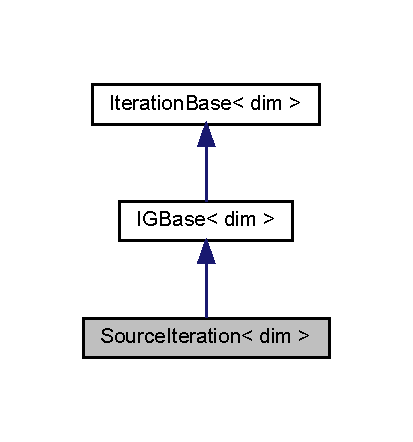
\includegraphics[width=198pt]{class_source_iteration__coll__graph}
\end{center}
\end{figure}
\subsection*{Public Member Functions}
\begin{DoxyCompactItemize}
\item 
\hyperlink{class_source_iteration_a50f7b38da2b8550f069386606026dc19}{Source\+Iteration} (const Parameter\+Handler \&prm)
\item 
\hyperlink{class_source_iteration_ae18057a8b8501d9e89b08ecfb33ef499}{$\sim$\+Source\+Iteration} ()
\begin{DoxyCompactList}\small\item\em Class destructor. \end{DoxyCompactList}\item 
void \hyperlink{class_source_iteration_a6d726b9a581391cc4164c29f4ccd1ca5}{solve\+\_\+in\+\_\+group} (std\+::vector$<$ Vector$<$ double $>$ $>$ \&sflxes\+\_\+proc, std\+\_\+cxx11\+::shared\+\_\+ptr$<$ \hyperlink{class_equation_base}{Equation\+Base}$<$ dim $>$ $>$ equ\+\_\+ptr, unsigned int \&g)
\end{DoxyCompactItemize}
\subsection*{Additional Inherited Members}


\subsection{Detailed Description}
\subsubsection*{template$<$int dim$>$\newline
class Source\+Iteration$<$ dim $>$}

This class provides source iteration scheme for in group solve. 

\begin{DoxyAuthor}{Author}
Weixiong Zheng 
\end{DoxyAuthor}
\begin{DoxyDate}{Date}
2017/08 
\end{DoxyDate}


Definition at line 64 of file ig\+\_\+base.\+h.



\subsection{Constructor \& Destructor Documentation}
\mbox{\Hypertarget{class_source_iteration_a50f7b38da2b8550f069386606026dc19}\label{class_source_iteration_a50f7b38da2b8550f069386606026dc19}} 
\index{Source\+Iteration@{Source\+Iteration}!Source\+Iteration@{Source\+Iteration}}
\index{Source\+Iteration@{Source\+Iteration}!Source\+Iteration@{Source\+Iteration}}
\subsubsection{\texorpdfstring{Source\+Iteration()}{SourceIteration()}}
{\footnotesize\ttfamily template$<$int dim$>$ \\
\hyperlink{class_source_iteration}{Source\+Iteration}$<$ dim $>$\+::\hyperlink{class_source_iteration}{Source\+Iteration} (\begin{DoxyParamCaption}\item[{const Parameter\+Handler \&}]{prm }\end{DoxyParamCaption})}

Class constructor.


\begin{DoxyParams}{Parameters}
{\em prm} & Const Parameter\+Handler object. \\
\hline
\end{DoxyParams}


Definition at line 27 of file ig\+\_\+base.\+cc.

\mbox{\Hypertarget{class_source_iteration_ae18057a8b8501d9e89b08ecfb33ef499}\label{class_source_iteration_ae18057a8b8501d9e89b08ecfb33ef499}} 
\index{Source\+Iteration@{Source\+Iteration}!````~Source\+Iteration@{$\sim$\+Source\+Iteration}}
\index{````~Source\+Iteration@{$\sim$\+Source\+Iteration}!Source\+Iteration@{Source\+Iteration}}
\subsubsection{\texorpdfstring{$\sim$\+Source\+Iteration()}{~SourceIteration()}}
{\footnotesize\ttfamily template$<$int dim$>$ \\
\hyperlink{class_source_iteration}{Source\+Iteration}$<$ dim $>$\+::$\sim$\hyperlink{class_source_iteration}{Source\+Iteration} (\begin{DoxyParamCaption}{ }\end{DoxyParamCaption})}



Class destructor. 



Definition at line 34 of file ig\+\_\+base.\+cc.



\subsection{Member Function Documentation}
\mbox{\Hypertarget{class_source_iteration_a6d726b9a581391cc4164c29f4ccd1ca5}\label{class_source_iteration_a6d726b9a581391cc4164c29f4ccd1ca5}} 
\index{Source\+Iteration@{Source\+Iteration}!solve\+\_\+in\+\_\+group@{solve\+\_\+in\+\_\+group}}
\index{solve\+\_\+in\+\_\+group@{solve\+\_\+in\+\_\+group}!Source\+Iteration@{Source\+Iteration}}
\subsubsection{\texorpdfstring{solve\+\_\+in\+\_\+group()}{solve\_in\_group()}}
{\footnotesize\ttfamily template$<$int dim$>$ \\
void \hyperlink{class_source_iteration}{Source\+Iteration}$<$ dim $>$\+::solve\+\_\+in\+\_\+group (\begin{DoxyParamCaption}\item[{std\+::vector$<$ Vector$<$ double $>$ $>$ \&}]{sflxes\+\_\+proc,  }\item[{std\+\_\+cxx11\+::shared\+\_\+ptr$<$ \hyperlink{class_equation_base}{Equation\+Base}$<$ dim $>$ $>$}]{equ\+\_\+ptr,  }\item[{unsigned int \&}]{g }\end{DoxyParamCaption})\hspace{0.3cm}{\ttfamily [virtual]}}

A function to solve SN in group using source iteration scheme.


\begin{DoxyParams}{Parameters}
{\em sflxes\+\_\+proc} & Scalar fluxes for all groups living on current processor. \\
\hline
{\em equ\+\_\+ptr} & A pointer to the equation of interest. \\
\hline
{\em g} & Group index. \\
\hline
\end{DoxyParams}


Reimplemented from \hyperlink{class_i_g_base_a902e919f8b0283be467261f94f79b2c4}{I\+G\+Base$<$ dim $>$}.



Definition at line 40 of file ig\+\_\+base.\+cc.



The documentation for this class was generated from the following files\+:\begin{DoxyCompactItemize}
\item 
src/iteration/\hyperlink{ig__base_8h}{ig\+\_\+base.\+h}\item 
src/iteration/\hyperlink{ig__base_8cc}{ig\+\_\+base.\+cc}\end{DoxyCompactItemize}

\chapter{File Documentation}
\hypertarget{aq__base_8cc}{}\section{src/aqdata/aq\+\_\+base.cc File Reference}
\label{aq__base_8cc}\index{src/aqdata/aq\+\_\+base.\+cc@{src/aqdata/aq\+\_\+base.\+cc}}
{\ttfamily \#include $<$deal.\+I\+I/base/numbers.\+h$>$}\newline
{\ttfamily \#include $<$fstream$>$}\newline
{\ttfamily \#include \char`\"{}aq\+\_\+base.\+h\char`\"{}}\newline
Include dependency graph for aq\+\_\+base.\+cc\+:\nopagebreak
\begin{figure}[H]
\begin{center}
\leavevmode
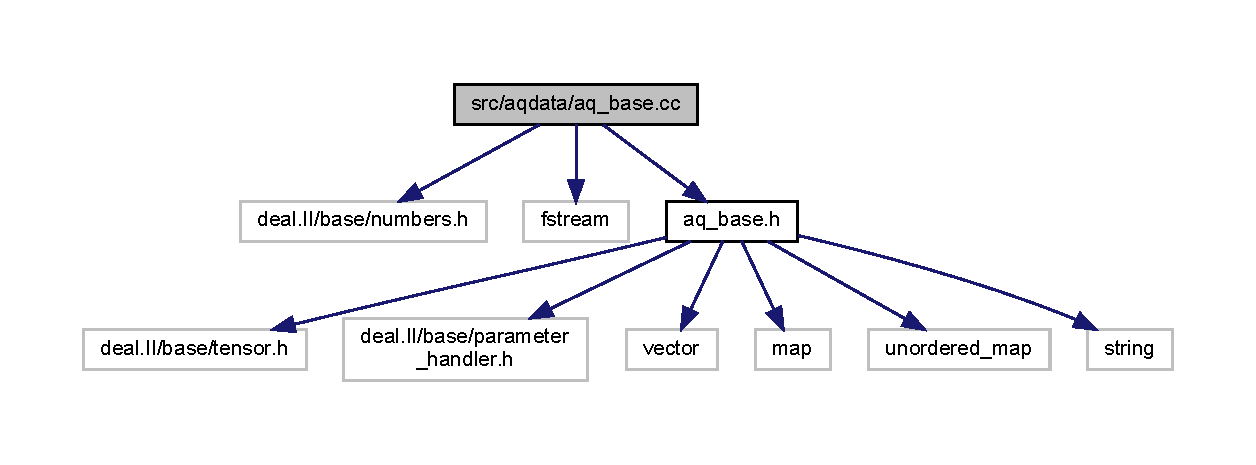
\includegraphics[width=350pt]{aq__base_8cc__incl}
\end{center}
\end{figure}

\hypertarget{aq__base_8h}{}\section{src/aqdata/aq\+\_\+base.h File Reference}
\label{aq__base_8h}\index{src/aqdata/aq\+\_\+base.\+h@{src/aqdata/aq\+\_\+base.\+h}}
{\ttfamily \#include $<$deal.\+I\+I/base/tensor.\+h$>$}\newline
{\ttfamily \#include $<$deal.\+I\+I/base/parameter\+\_\+handler.\+h$>$}\newline
{\ttfamily \#include $<$vector$>$}\newline
{\ttfamily \#include $<$map$>$}\newline
{\ttfamily \#include $<$unordered\+\_\+map$>$}\newline
{\ttfamily \#include $<$string$>$}\newline
Include dependency graph for aq\+\_\+base.\+h\+:\nopagebreak
\begin{figure}[H]
\begin{center}
\leavevmode
\includegraphics[width=350pt]{aq__base_8h__incl}
\end{center}
\end{figure}
This graph shows which files directly or indirectly include this file\+:\nopagebreak
\begin{figure}[H]
\begin{center}
\leavevmode
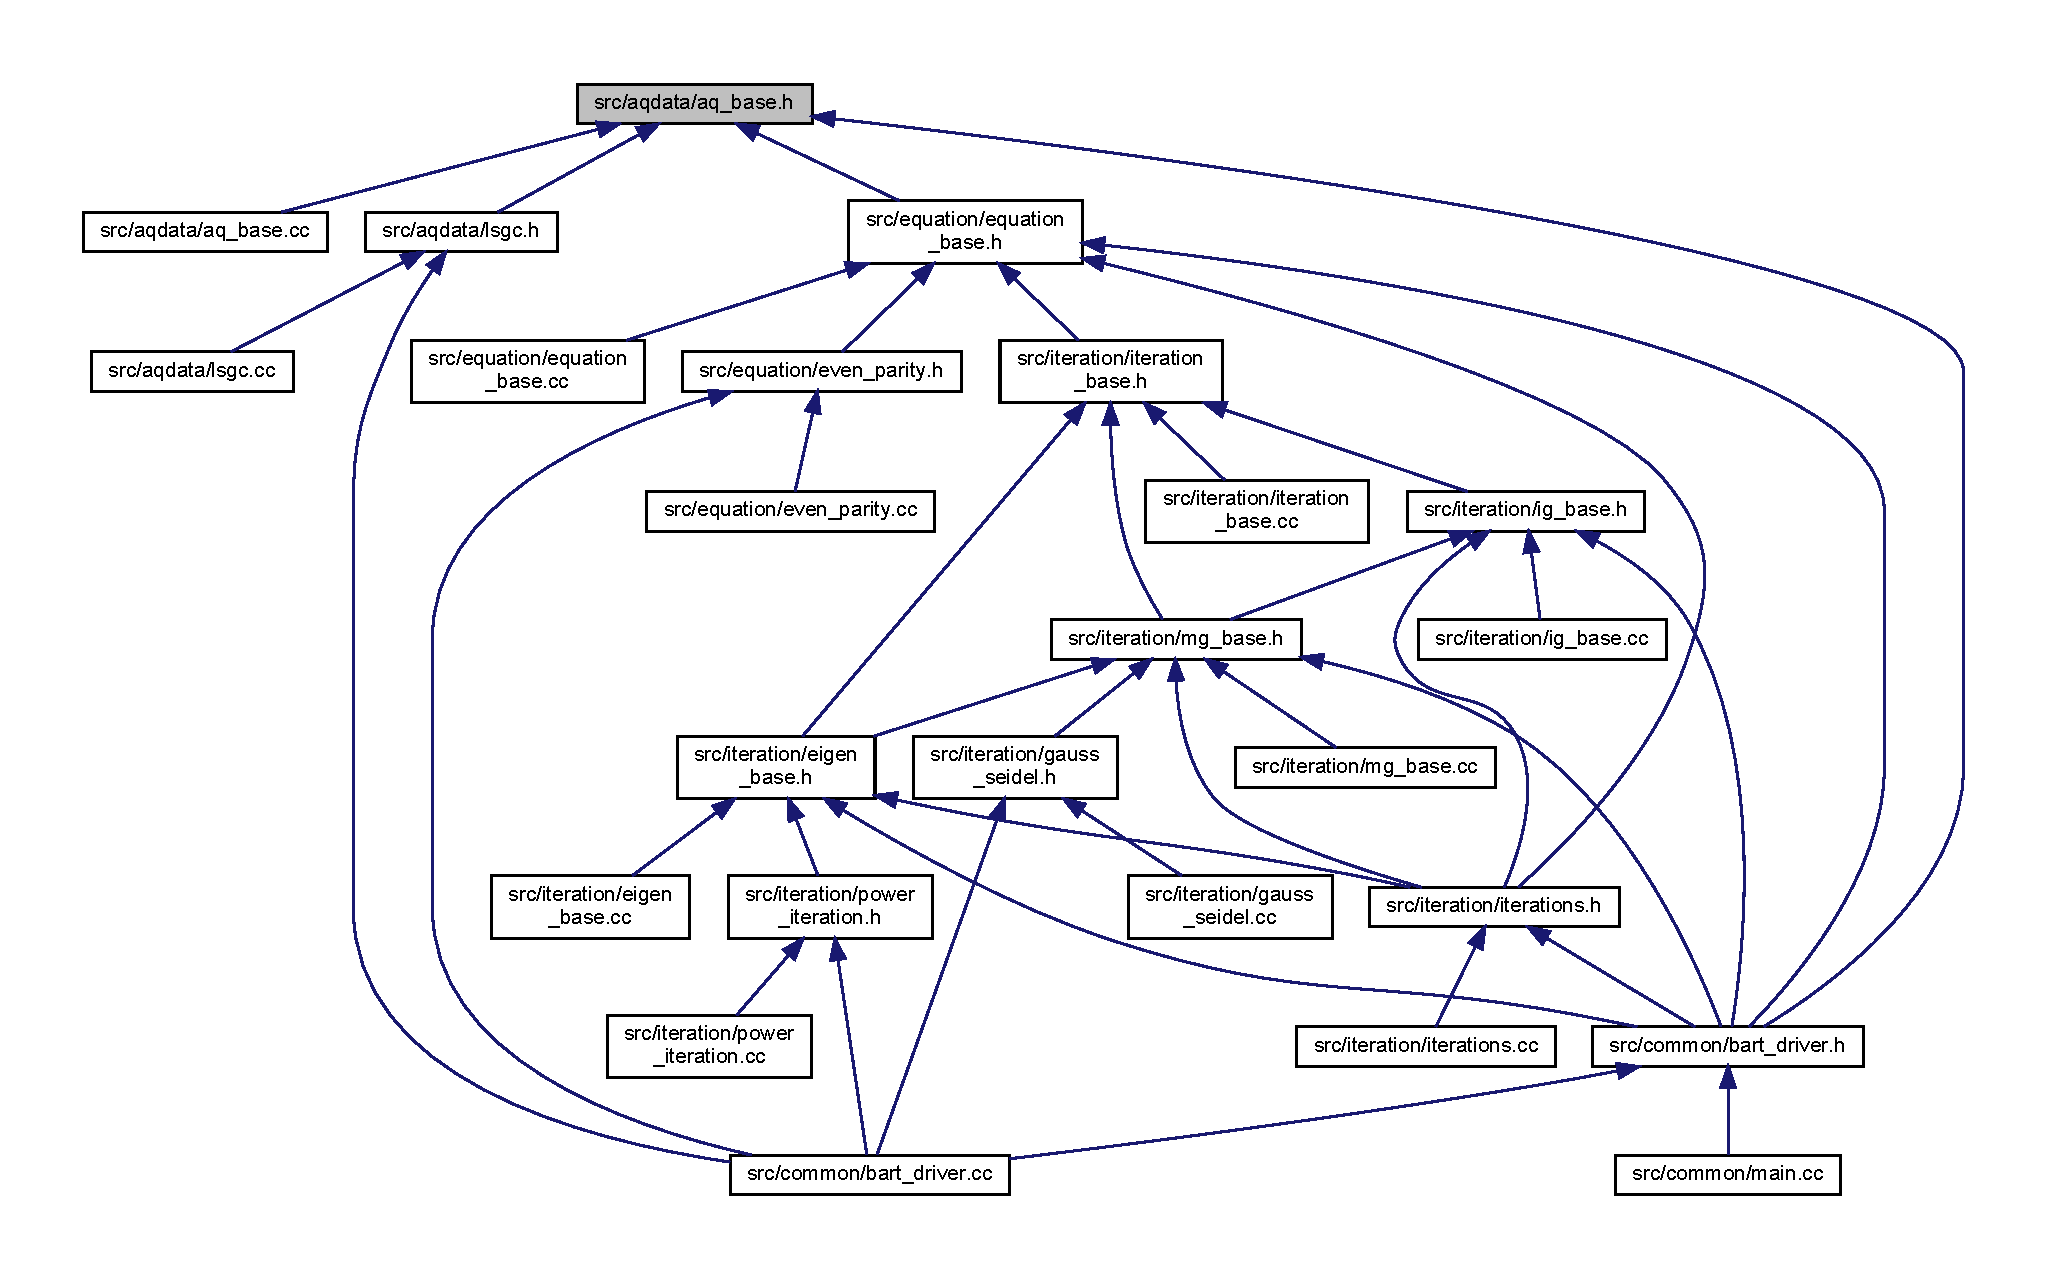
\includegraphics[width=350pt]{aq__base_8h__dep__incl}
\end{center}
\end{figure}
\subsection*{Classes}
\begin{DoxyCompactItemize}
\item 
class \hyperlink{class_a_q_base}{A\+Q\+Base$<$ dim $>$}
\begin{DoxyCompactList}\small\item\em This class provides AQ data, component indices and reflective directions. \end{DoxyCompactList}\end{DoxyCompactItemize}

\hypertarget{lsgc_8cc}{}\section{src/aqdata/lsgc.cc File Reference}
\label{lsgc_8cc}\index{src/aqdata/lsgc.\+cc@{src/aqdata/lsgc.\+cc}}
{\ttfamily \#include $<$deal.\+I\+I/base/quadrature\+\_\+lib.\+h$>$}\newline
{\ttfamily \#include $<$iostream$>$}\newline
{\ttfamily \#include \char`\"{}lsgc.\+h\char`\"{}}\newline
Include dependency graph for lsgc.\+cc\+:\nopagebreak
\begin{figure}[H]
\begin{center}
\leavevmode
\includegraphics[width=350pt]{lsgc_8cc__incl}
\end{center}
\end{figure}

\hypertarget{lsgc_8h}{}\section{src/aqdata/lsgc.h File Reference}
\label{lsgc_8h}\index{src/aqdata/lsgc.\+h@{src/aqdata/lsgc.\+h}}
{\ttfamily \#include \char`\"{}aq\+\_\+base.\+h\char`\"{}}\newline
Include dependency graph for lsgc.\+h\+:\nopagebreak
\begin{figure}[H]
\begin{center}
\leavevmode
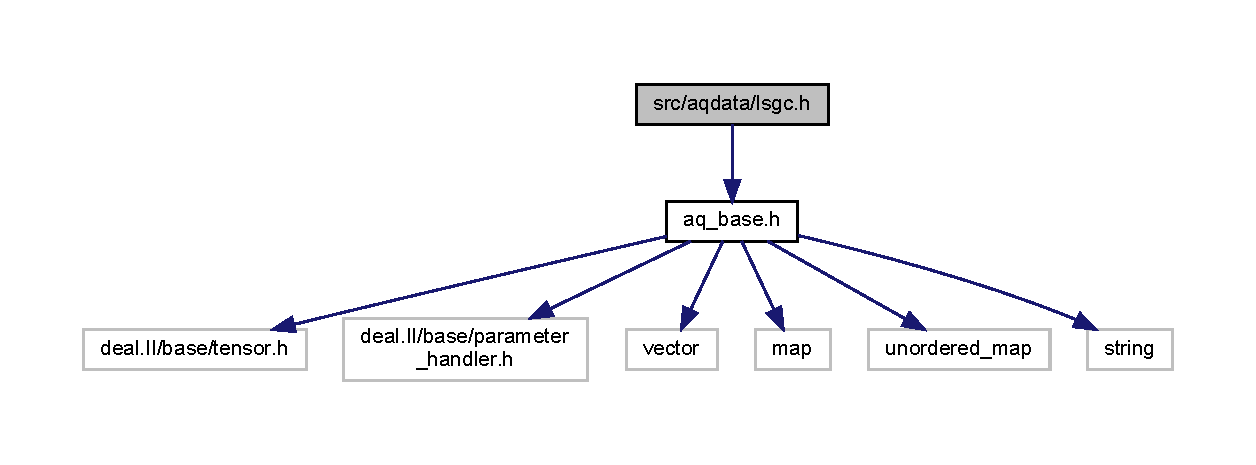
\includegraphics[width=350pt]{lsgc_8h__incl}
\end{center}
\end{figure}
This graph shows which files directly or indirectly include this file\+:\nopagebreak
\begin{figure}[H]
\begin{center}
\leavevmode
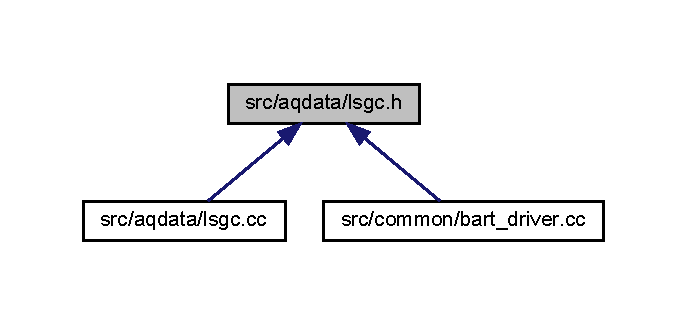
\includegraphics[width=330pt]{lsgc_8h__dep__incl}
\end{center}
\end{figure}
\subsection*{Classes}
\begin{DoxyCompactItemize}
\item 
class \hyperlink{class_l_s_g_c}{L\+S\+G\+C$<$ dim $>$}
\begin{DoxyCompactList}\small\item\em This class produces level-\/symmetric Gauss-\/\+Chebyshev quadrature. \end{DoxyCompactList}\end{DoxyCompactItemize}

\hypertarget{bart__driver_8cc}{}\section{src/common/bart\+\_\+driver.cc File Reference}
\label{bart__driver_8cc}\index{src/common/bart\+\_\+driver.\+cc@{src/common/bart\+\_\+driver.\+cc}}
{\ttfamily \#include $<$deal.\+I\+I/fe/fe\+\_\+dgq.\+h$>$}\newline
{\ttfamily \#include $<$deal.\+I\+I/fe/fe\+\_\+q.\+h$>$}\newline
{\ttfamily \#include $<$deal.\+I\+I/dofs/dof\+\_\+tools.\+h$>$}\newline
{\ttfamily \#include $<$deal.\+I\+I/base/utilities.\+h$>$}\newline
{\ttfamily \#include $<$algorithm$>$}\newline
{\ttfamily \#include $<$fstream$>$}\newline
{\ttfamily \#include $<$sstream$>$}\newline
{\ttfamily \#include \char`\"{}bart\+\_\+driver.\+h\char`\"{}}\newline
{\ttfamily \#include \char`\"{}../aqdata/lsgc.\+h\char`\"{}}\newline
{\ttfamily \#include \char`\"{}../equation/even\+\_\+parity.\+h\char`\"{}}\newline
{\ttfamily \#include \char`\"{}../iteration/power\+\_\+iteration.\+h\char`\"{}}\newline
{\ttfamily \#include \char`\"{}../iteration/gauss\+\_\+seidel.\+h\char`\"{}}\newline
Include dependency graph for bart\+\_\+driver.\+cc\+:\nopagebreak
\begin{figure}[H]
\begin{center}
\leavevmode
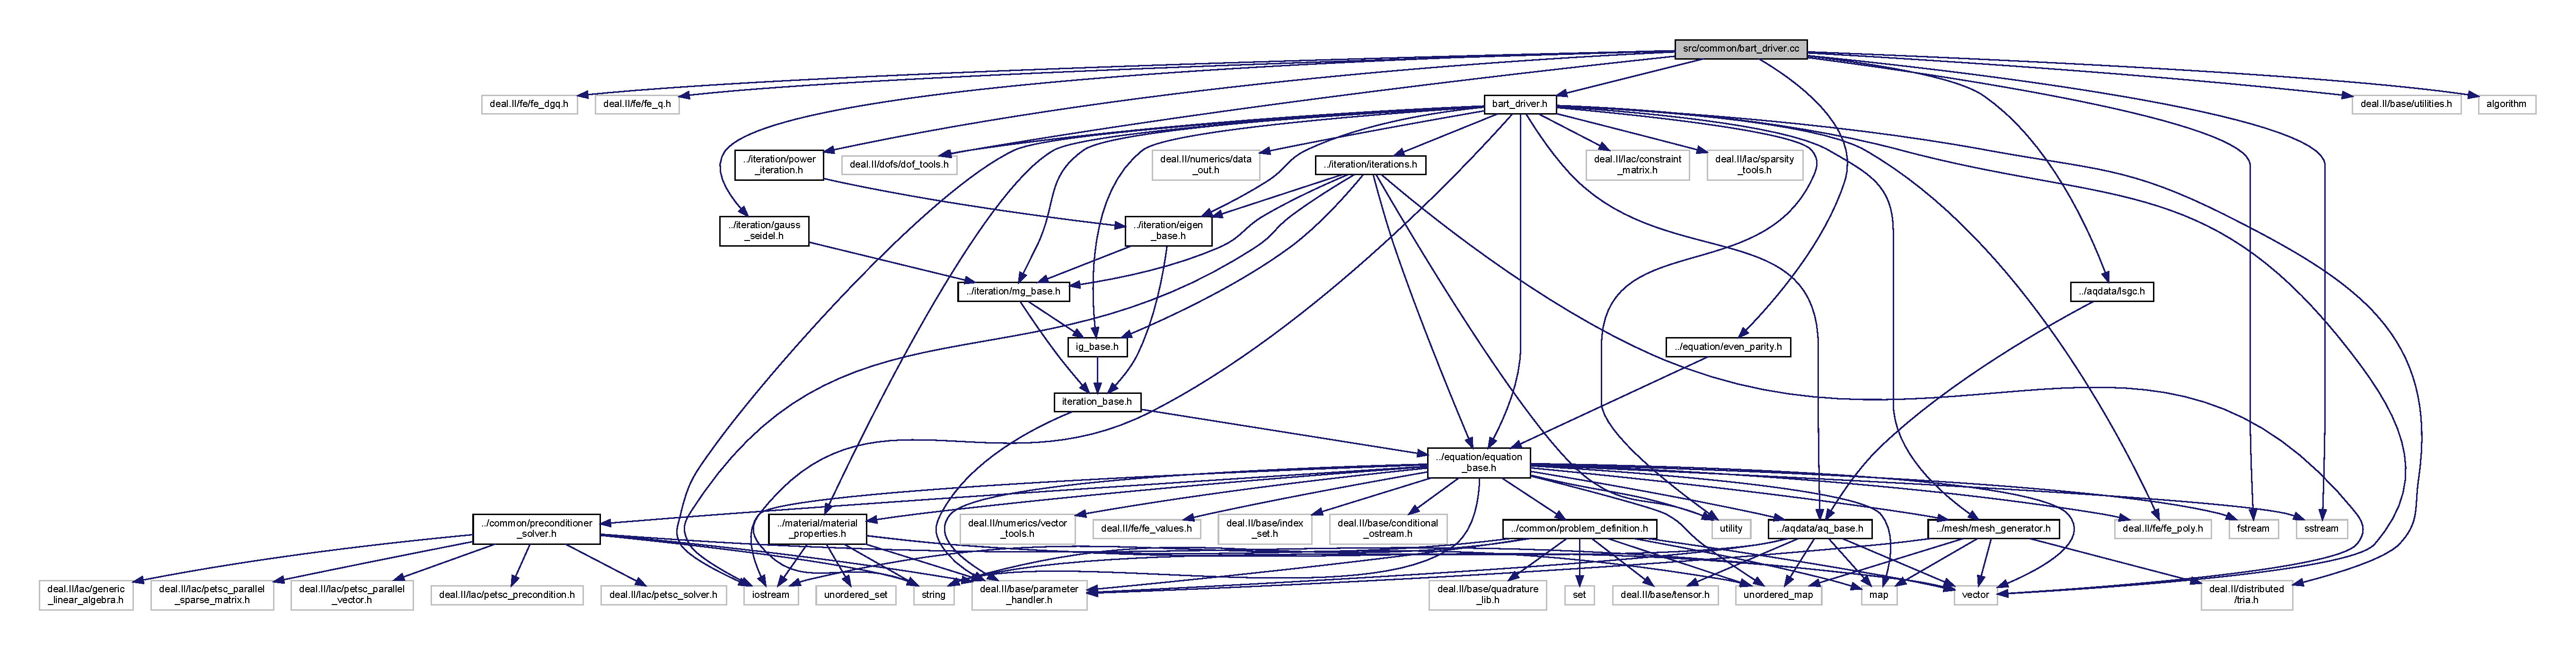
\includegraphics[width=350pt]{bart__driver_8cc__incl}
\end{center}
\end{figure}

\hypertarget{bart__driver_8h}{}\section{src/common/bart\+\_\+driver.h File Reference}
\label{bart__driver_8h}\index{src/common/bart\+\_\+driver.\+h@{src/common/bart\+\_\+driver.\+h}}
{\ttfamily \#include $<$deal.\+I\+I/lac/constraint\+\_\+matrix.\+h$>$}\newline
{\ttfamily \#include $<$deal.\+I\+I/lac/sparsity\+\_\+tools.\+h$>$}\newline
{\ttfamily \#include $<$deal.\+I\+I/fe/fe\+\_\+poly.\+h$>$}\newline
{\ttfamily \#include $<$deal.\+I\+I/dofs/dof\+\_\+tools.\+h$>$}\newline
{\ttfamily \#include $<$deal.\+I\+I/distributed/tria.\+h$>$}\newline
{\ttfamily \#include $<$deal.\+I\+I/numerics/data\+\_\+out.\+h$>$}\newline
{\ttfamily \#include $<$iostream$>$}\newline
{\ttfamily \#include $<$string$>$}\newline
{\ttfamily \#include $<$utility$>$}\newline
{\ttfamily \#include $<$vector$>$}\newline
{\ttfamily \#include \char`\"{}../mesh/mesh\+\_\+generator.\+h\char`\"{}}\newline
{\ttfamily \#include \char`\"{}../material/material\+\_\+properties.\+h\char`\"{}}\newline
{\ttfamily \#include \char`\"{}../aqdata/aq\+\_\+base.\+h\char`\"{}}\newline
{\ttfamily \#include \char`\"{}../equation/equation\+\_\+base.\+h\char`\"{}}\newline
{\ttfamily \#include \char`\"{}../iteration/mg\+\_\+base.\+h\char`\"{}}\newline
{\ttfamily \#include \char`\"{}../iteration/ig\+\_\+base.\+h\char`\"{}}\newline
{\ttfamily \#include \char`\"{}../iteration/eigen\+\_\+base.\+h\char`\"{}}\newline
{\ttfamily \#include \char`\"{}../iteration/iterations.\+h\char`\"{}}\newline
Include dependency graph for bart\+\_\+driver.\+h\+:\nopagebreak
\begin{figure}[H]
\begin{center}
\leavevmode
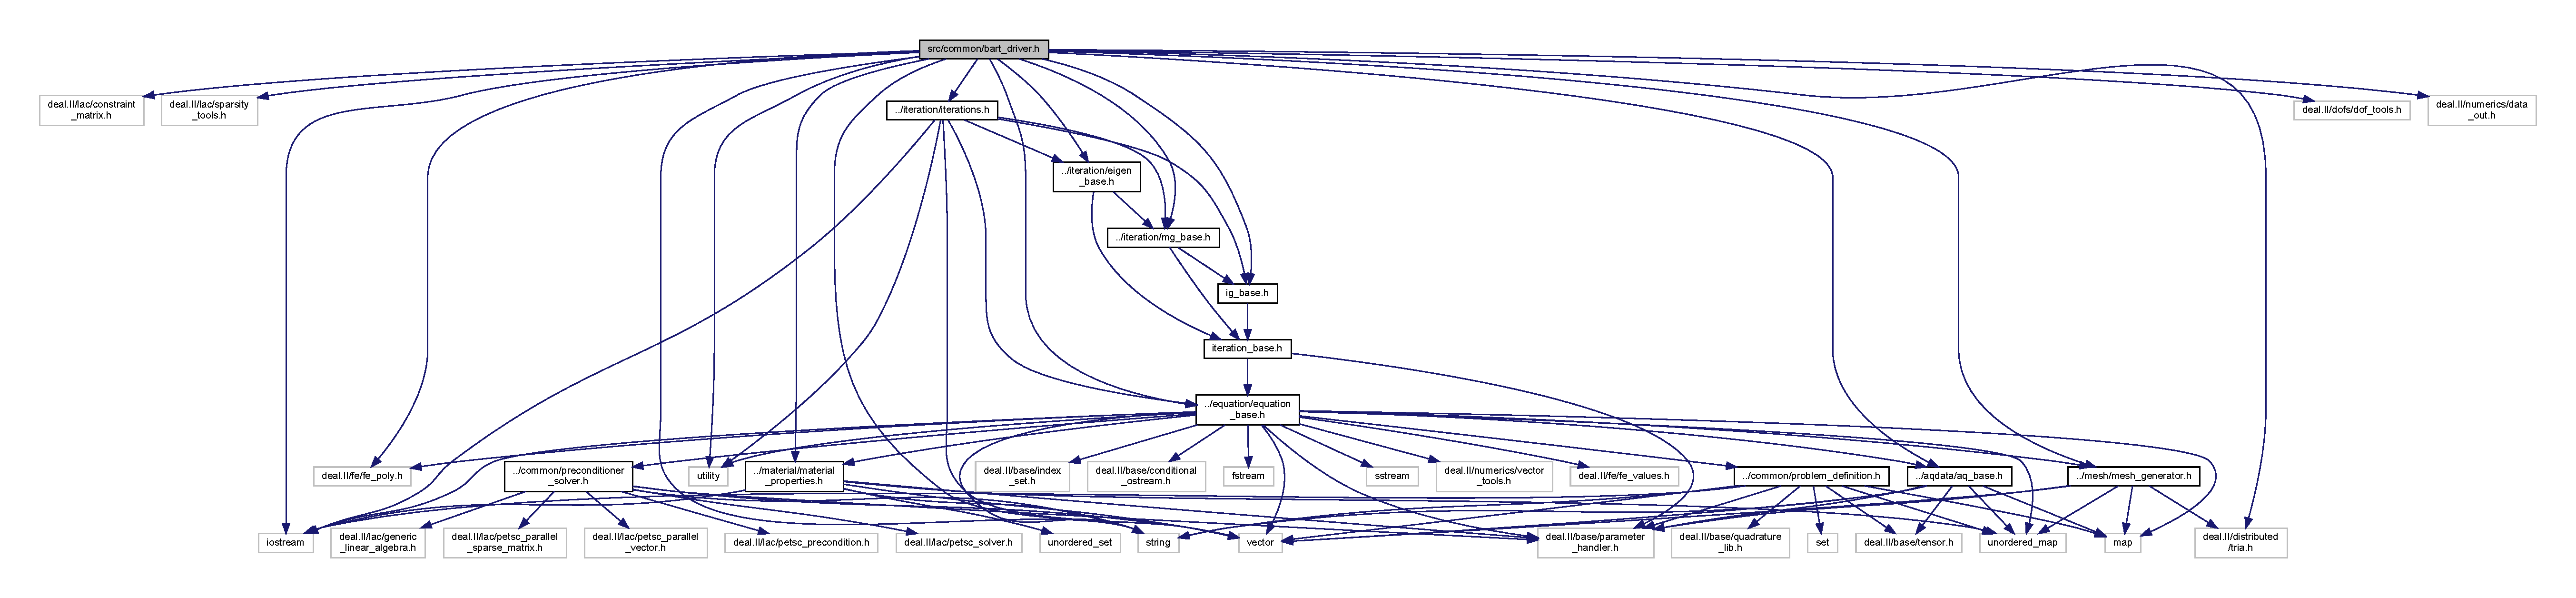
\includegraphics[width=350pt]{bart__driver_8h__incl}
\end{center}
\end{figure}
This graph shows which files directly or indirectly include this file\+:\nopagebreak
\begin{figure}[H]
\begin{center}
\leavevmode
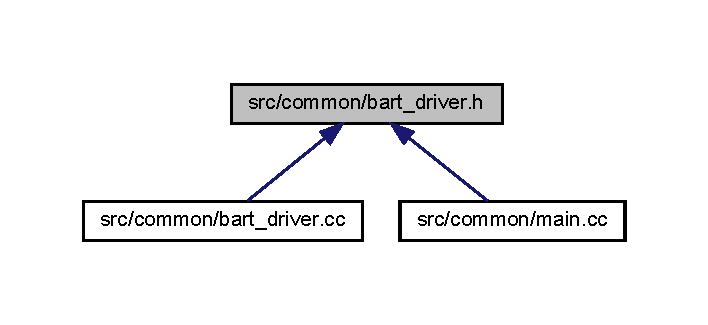
\includegraphics[width=340pt]{bart__driver_8h__dep__incl}
\end{center}
\end{figure}
\subsection*{Classes}
\begin{DoxyCompactItemize}
\item 
class \hyperlink{class_bart_driver}{Bart\+Driver$<$ dim $>$}
\begin{DoxyCompactList}\small\item\em This class provides highest-\/level operations on B\+A\+RT to solve the problems. \end{DoxyCompactList}\end{DoxyCompactItemize}

\hypertarget{main_8cc}{}\section{src/common/main.cc File Reference}
\label{main_8cc}\index{src/common/main.\+cc@{src/common/main.\+cc}}
{\ttfamily \#include $<$deal.\+I\+I/base/utilities.\+h$>$}\newline
{\ttfamily \#include $<$deal.\+I\+I/base/mpi.\+h$>$}\newline
{\ttfamily \#include \char`\"{}problem\+\_\+definition.\+h\char`\"{}}\newline
{\ttfamily \#include \char`\"{}bart\+\_\+driver.\+h\char`\"{}}\newline
Include dependency graph for main.\+cc\+:\nopagebreak
\begin{figure}[H]
\begin{center}
\leavevmode
\includegraphics[width=350pt]{main_8cc__incl}
\end{center}
\end{figure}
\subsection*{Functions}
\begin{DoxyCompactItemize}
\item 
int \hyperlink{main_8cc_a0ddf1224851353fc92bfbff6f499fa97}{main} (int argc, char $\ast$argv\mbox{[}$\,$\mbox{]})
\end{DoxyCompactItemize}


\subsection{Function Documentation}
\mbox{\Hypertarget{main_8cc_a0ddf1224851353fc92bfbff6f499fa97}\label{main_8cc_a0ddf1224851353fc92bfbff6f499fa97}} 
\index{main.\+cc@{main.\+cc}!main@{main}}
\index{main@{main}!main.\+cc@{main.\+cc}}
\subsubsection{\texorpdfstring{main()}{main()}}
{\footnotesize\ttfamily int main (\begin{DoxyParamCaption}\item[{int}]{argc,  }\item[{char $\ast$}]{argv\mbox{[}$\,$\mbox{]} }\end{DoxyParamCaption})}



Definition at line 17 of file main.\+cc.

Here is the call graph for this function\+:\nopagebreak
\begin{figure}[H]
\begin{center}
\leavevmode
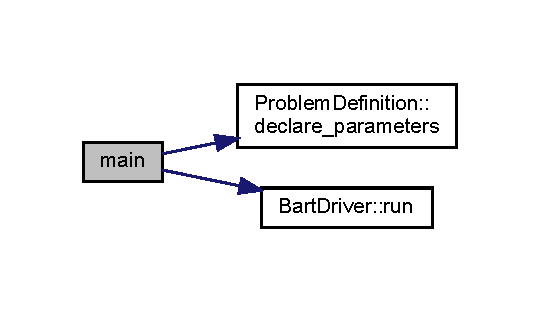
\includegraphics[width=259pt]{main_8cc_a0ddf1224851353fc92bfbff6f499fa97_cgraph}
\end{center}
\end{figure}

\hypertarget{preconditioner__solver_8cc}{}\section{src/common/preconditioner\+\_\+solver.cc File Reference}
\label{preconditioner__solver_8cc}\index{src/common/preconditioner\+\_\+solver.\+cc@{src/common/preconditioner\+\_\+solver.\+cc}}
{\ttfamily \#include \char`\"{}preconditioner\+\_\+solver.\+h\char`\"{}}\newline
Include dependency graph for preconditioner\+\_\+solver.\+cc\+:\nopagebreak
\begin{figure}[H]
\begin{center}
\leavevmode
\includegraphics[width=350pt]{preconditioner__solver_8cc__incl}
\end{center}
\end{figure}

\hypertarget{preconditioner__solver_8h}{}\section{src/common/preconditioner\+\_\+solver.h File Reference}
\label{preconditioner__solver_8h}\index{src/common/preconditioner\+\_\+solver.\+h@{src/common/preconditioner\+\_\+solver.\+h}}
{\ttfamily \#include $<$deal.\+I\+I/lac/generic\+\_\+linear\+\_\+algebra.\+h$>$}\newline
{\ttfamily \#include $<$deal.\+I\+I/lac/petsc\+\_\+parallel\+\_\+sparse\+\_\+matrix.\+h$>$}\newline
{\ttfamily \#include $<$deal.\+I\+I/lac/petsc\+\_\+parallel\+\_\+vector.\+h$>$}\newline
{\ttfamily \#include $<$deal.\+I\+I/lac/petsc\+\_\+precondition.\+h$>$}\newline
{\ttfamily \#include $<$deal.\+I\+I/lac/petsc\+\_\+solver.\+h$>$}\newline
{\ttfamily \#include $<$deal.\+I\+I/base/parameter\+\_\+handler.\+h$>$}\newline
{\ttfamily \#include $<$vector$>$}\newline
{\ttfamily \#include $<$string$>$}\newline
Include dependency graph for preconditioner\+\_\+solver.\+h\+:\nopagebreak
\begin{figure}[H]
\begin{center}
\leavevmode
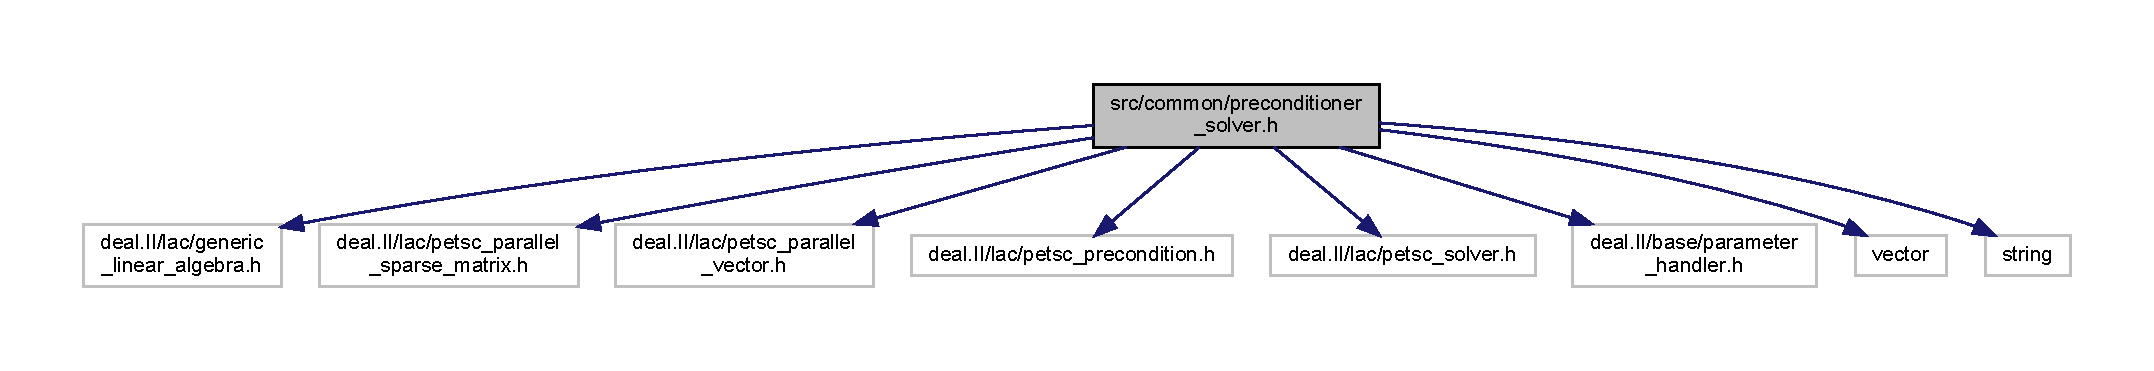
\includegraphics[width=350pt]{preconditioner__solver_8h__incl}
\end{center}
\end{figure}
This graph shows which files directly or indirectly include this file\+:\nopagebreak
\begin{figure}[H]
\begin{center}
\leavevmode
\includegraphics[width=350pt]{preconditioner__solver_8h__dep__incl}
\end{center}
\end{figure}
\subsection*{Classes}
\begin{DoxyCompactItemize}
\item 
class \hyperlink{class_preconditioner_solver}{Preconditioner\+Solver}
\begin{DoxyCompactList}\small\item\em The class provides linear solving functionalities. \end{DoxyCompactList}\end{DoxyCompactItemize}

\hypertarget{problem__definition_8cc}{}\section{src/common/problem\+\_\+definition.cc File Reference}
\label{problem__definition_8cc}\index{src/common/problem\+\_\+definition.\+cc@{src/common/problem\+\_\+definition.\+cc}}
{\ttfamily \#include $<$deal.\+I\+I/base/utilities.\+h$>$}\newline
{\ttfamily \#include $<$sstream$>$}\newline
{\ttfamily \#include $<$utility$>$}\newline
{\ttfamily \#include $<$iomanip$>$}\newline
{\ttfamily \#include \char`\"{}problem\+\_\+definition.\+h\char`\"{}}\newline
Include dependency graph for problem\+\_\+definition.\+cc\+:\nopagebreak
\begin{figure}[H]
\begin{center}
\leavevmode
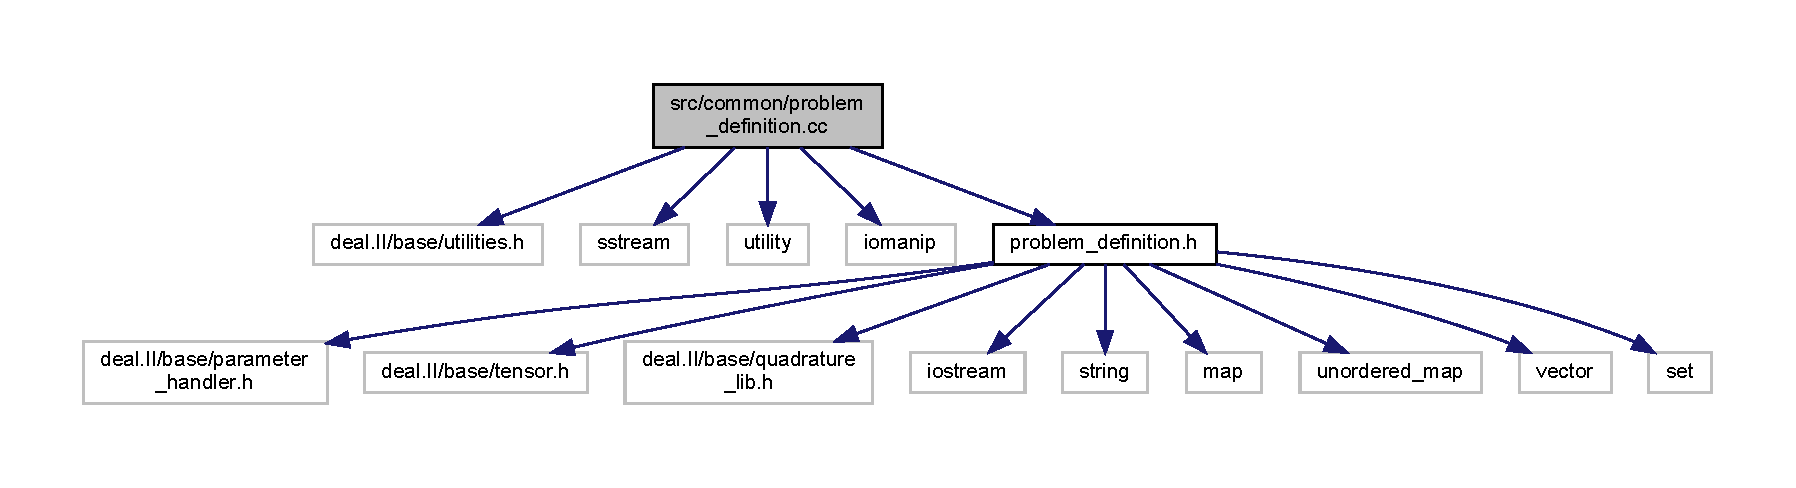
\includegraphics[width=350pt]{problem__definition_8cc__incl}
\end{center}
\end{figure}

\hypertarget{problem__definition_8h}{}\section{src/common/problem\+\_\+definition.h File Reference}
\label{problem__definition_8h}\index{src/common/problem\+\_\+definition.\+h@{src/common/problem\+\_\+definition.\+h}}
{\ttfamily \#include $<$deal.\+I\+I/base/parameter\+\_\+handler.\+h$>$}\newline
{\ttfamily \#include $<$deal.\+I\+I/base/tensor.\+h$>$}\newline
{\ttfamily \#include $<$deal.\+I\+I/base/quadrature\+\_\+lib.\+h$>$}\newline
{\ttfamily \#include $<$iostream$>$}\newline
{\ttfamily \#include $<$string$>$}\newline
{\ttfamily \#include $<$map$>$}\newline
{\ttfamily \#include $<$unordered\+\_\+map$>$}\newline
{\ttfamily \#include $<$vector$>$}\newline
{\ttfamily \#include $<$set$>$}\newline
Include dependency graph for problem\+\_\+definition.\+h\+:\nopagebreak
\begin{figure}[H]
\begin{center}
\leavevmode
\includegraphics[width=350pt]{problem__definition_8h__incl}
\end{center}
\end{figure}
This graph shows which files directly or indirectly include this file\+:\nopagebreak
\begin{figure}[H]
\begin{center}
\leavevmode
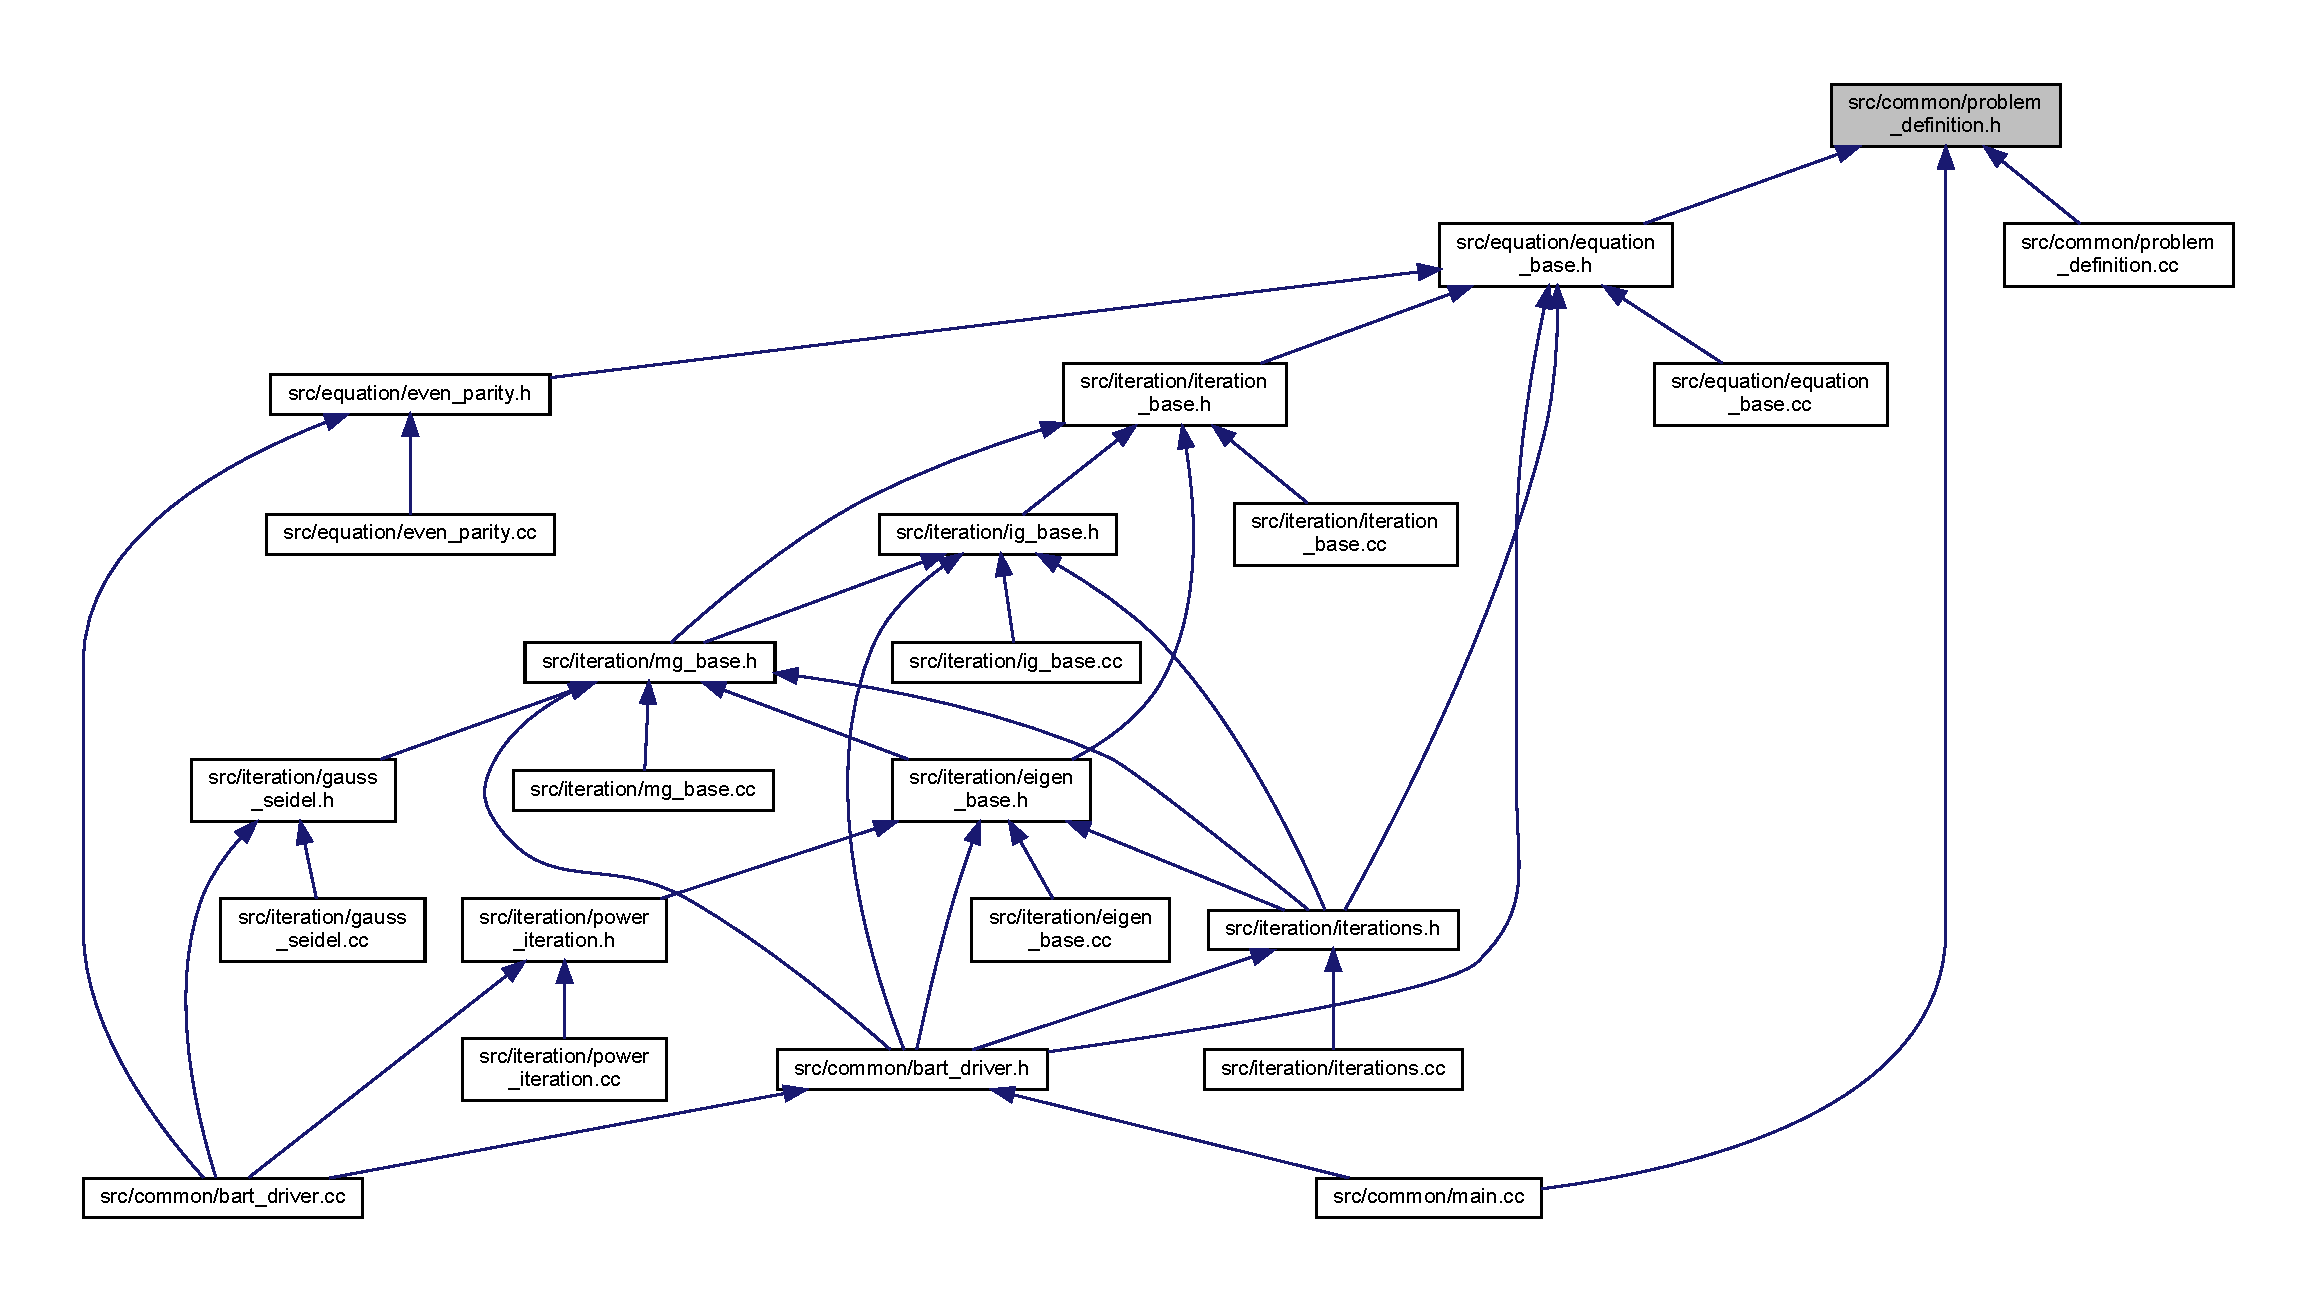
\includegraphics[width=350pt]{problem__definition_8h__dep__incl}
\end{center}
\end{figure}
\subsection*{Classes}
\begin{DoxyCompactItemize}
\item 
class \hyperlink{class_problem_definition}{Problem\+Definition}
\begin{DoxyCompactList}\small\item\em This class performs parameter parsing. \end{DoxyCompactList}\end{DoxyCompactItemize}
\subsection*{Variables}
\begin{DoxyCompactItemize}
\item 
const unsigned int \hyperlink{problem__definition_8h_a39bfd9bc6997aad2801f2fde347a16f1}{nmat} = 50
\item 
const unsigned int \hyperlink{problem__definition_8h_a0dbbc66524fa33586544e439fe513771}{ngrp} = 30
\item 
const unsigned int \hyperlink{problem__definition_8h_a36fc3e04ecb4cc483c34cb452808b403}{z\+\_\+levels} = 30
\item 
const unsigned int \hyperlink{problem__definition_8h_af4a3617b651fff9cd04a28e714263b80}{y\+\_\+levels} = 100
\end{DoxyCompactItemize}


\subsection{Variable Documentation}
\mbox{\Hypertarget{problem__definition_8h_a0dbbc66524fa33586544e439fe513771}\label{problem__definition_8h_a0dbbc66524fa33586544e439fe513771}} 
\index{problem\+\_\+definition.\+h@{problem\+\_\+definition.\+h}!ngrp@{ngrp}}
\index{ngrp@{ngrp}!problem\+\_\+definition.\+h@{problem\+\_\+definition.\+h}}
\subsubsection{\texorpdfstring{ngrp}{ngrp}}
{\footnotesize\ttfamily const unsigned int ngrp = 30}



Definition at line 18 of file problem\+\_\+definition.\+h.

\mbox{\Hypertarget{problem__definition_8h_a39bfd9bc6997aad2801f2fde347a16f1}\label{problem__definition_8h_a39bfd9bc6997aad2801f2fde347a16f1}} 
\index{problem\+\_\+definition.\+h@{problem\+\_\+definition.\+h}!nmat@{nmat}}
\index{nmat@{nmat}!problem\+\_\+definition.\+h@{problem\+\_\+definition.\+h}}
\subsubsection{\texorpdfstring{nmat}{nmat}}
{\footnotesize\ttfamily const unsigned int nmat = 50}



Definition at line 17 of file problem\+\_\+definition.\+h.

\mbox{\Hypertarget{problem__definition_8h_af4a3617b651fff9cd04a28e714263b80}\label{problem__definition_8h_af4a3617b651fff9cd04a28e714263b80}} 
\index{problem\+\_\+definition.\+h@{problem\+\_\+definition.\+h}!y\+\_\+levels@{y\+\_\+levels}}
\index{y\+\_\+levels@{y\+\_\+levels}!problem\+\_\+definition.\+h@{problem\+\_\+definition.\+h}}
\subsubsection{\texorpdfstring{y\+\_\+levels}{y\_levels}}
{\footnotesize\ttfamily const unsigned int y\+\_\+levels = 100}



Definition at line 20 of file problem\+\_\+definition.\+h.

\mbox{\Hypertarget{problem__definition_8h_a36fc3e04ecb4cc483c34cb452808b403}\label{problem__definition_8h_a36fc3e04ecb4cc483c34cb452808b403}} 
\index{problem\+\_\+definition.\+h@{problem\+\_\+definition.\+h}!z\+\_\+levels@{z\+\_\+levels}}
\index{z\+\_\+levels@{z\+\_\+levels}!problem\+\_\+definition.\+h@{problem\+\_\+definition.\+h}}
\subsubsection{\texorpdfstring{z\+\_\+levels}{z\_levels}}
{\footnotesize\ttfamily const unsigned int z\+\_\+levels = 30}



Definition at line 19 of file problem\+\_\+definition.\+h.


\hypertarget{equation__base_8cc}{}\section{src/equation/equation\+\_\+base.cc File Reference}
\label{equation__base_8cc}\index{src/equation/equation\+\_\+base.\+cc@{src/equation/equation\+\_\+base.\+cc}}
{\ttfamily \#include $<$deal.\+I\+I/dofs/dof\+\_\+tools.\+h$>$}\newline
{\ttfamily \#include $<$deal.\+I\+I/grid/cell\+\_\+id.\+h$>$}\newline
{\ttfamily \#include $<$deal.\+I\+I/base/utilities.\+h$>$}\newline
{\ttfamily \#include $<$algorithm$>$}\newline
{\ttfamily \#include $<$fstream$>$}\newline
{\ttfamily \#include \char`\"{}equation\+\_\+base.\+h\char`\"{}}\newline
Include dependency graph for equation\+\_\+base.\+cc\+:\nopagebreak
\begin{figure}[H]
\begin{center}
\leavevmode
\includegraphics[width=350pt]{equation__base_8cc__incl}
\end{center}
\end{figure}

\hypertarget{equation__base_8h}{}\section{src/equation/equation\+\_\+base.h File Reference}
\label{equation__base_8h}\index{src/equation/equation\+\_\+base.\+h@{src/equation/equation\+\_\+base.\+h}}
{\ttfamily \#include $<$deal.\+I\+I/numerics/vector\+\_\+tools.\+h$>$}\newline
{\ttfamily \#include $<$deal.\+I\+I/fe/fe\+\_\+poly.\+h$>$}\newline
{\ttfamily \#include $<$deal.\+I\+I/fe/fe\+\_\+values.\+h$>$}\newline
{\ttfamily \#include $<$deal.\+I\+I/base/parameter\+\_\+handler.\+h$>$}\newline
{\ttfamily \#include $<$deal.\+I\+I/base/index\+\_\+set.\+h$>$}\newline
{\ttfamily \#include $<$deal.\+I\+I/base/conditional\+\_\+ostream.\+h$>$}\newline
{\ttfamily \#include $<$fstream$>$}\newline
{\ttfamily \#include $<$iostream$>$}\newline
{\ttfamily \#include $<$sstream$>$}\newline
{\ttfamily \#include $<$string$>$}\newline
{\ttfamily \#include $<$map$>$}\newline
{\ttfamily \#include $<$unordered\+\_\+map$>$}\newline
{\ttfamily \#include $<$utility$>$}\newline
{\ttfamily \#include $<$vector$>$}\newline
{\ttfamily \#include \char`\"{}../common/problem\+\_\+definition.\+h\char`\"{}}\newline
{\ttfamily \#include \char`\"{}../common/preconditioner\+\_\+solver.\+h\char`\"{}}\newline
{\ttfamily \#include \char`\"{}../mesh/mesh\+\_\+generator.\+h\char`\"{}}\newline
{\ttfamily \#include \char`\"{}../material/material\+\_\+properties.\+h\char`\"{}}\newline
{\ttfamily \#include \char`\"{}../aqdata/aq\+\_\+base.\+h\char`\"{}}\newline
Include dependency graph for equation\+\_\+base.\+h\+:\nopagebreak
\begin{figure}[H]
\begin{center}
\leavevmode
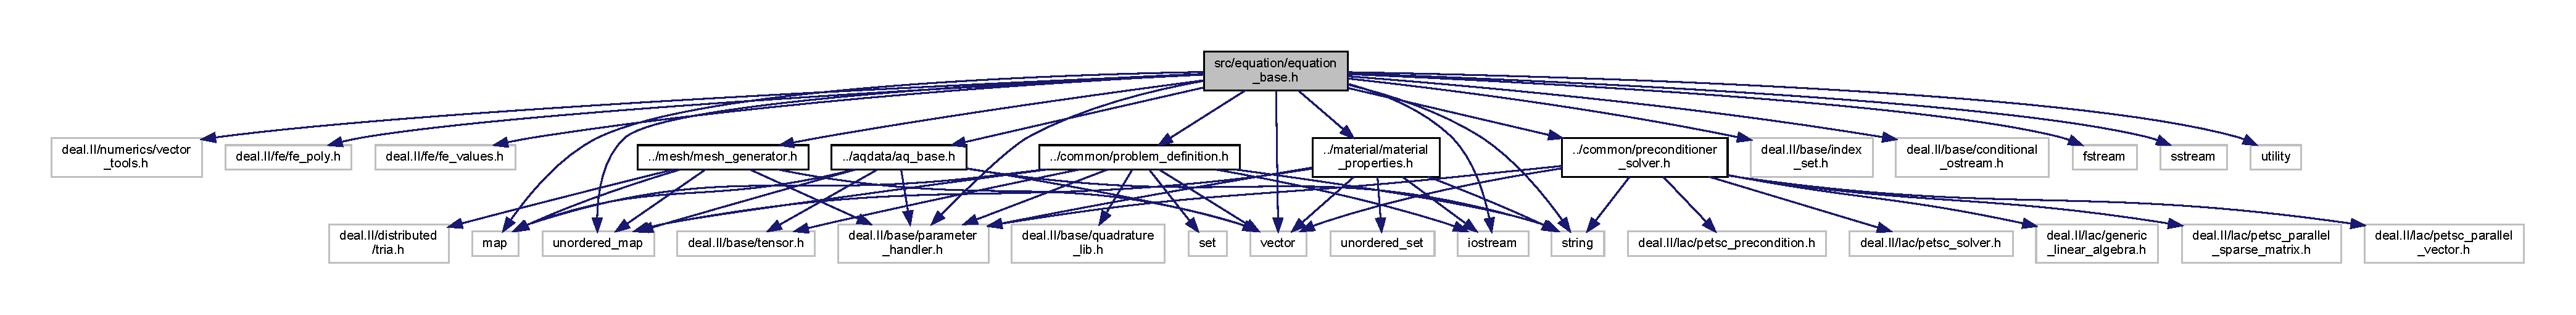
\includegraphics[width=350pt]{equation__base_8h__incl}
\end{center}
\end{figure}
This graph shows which files directly or indirectly include this file\+:\nopagebreak
\begin{figure}[H]
\begin{center}
\leavevmode
\includegraphics[width=350pt]{equation__base_8h__dep__incl}
\end{center}
\end{figure}
\subsection*{Classes}
\begin{DoxyCompactItemize}
\item 
class \hyperlink{class_equation_base}{Equation\+Base$<$ dim $>$}
\begin{DoxyCompactList}\small\item\em This class provides weak form assembly and physical quantity computation functionalities. \end{DoxyCompactList}\end{DoxyCompactItemize}

\hypertarget{even__parity_8cc}{}\section{src/equation/even\+\_\+parity.cc File Reference}
\label{even__parity_8cc}\index{src/equation/even\+\_\+parity.\+cc@{src/equation/even\+\_\+parity.\+cc}}
{\ttfamily \#include \char`\"{}even\+\_\+parity.\+h\char`\"{}}\newline
Include dependency graph for even\+\_\+parity.\+cc\+:\nopagebreak
\begin{figure}[H]
\begin{center}
\leavevmode
\includegraphics[width=350pt]{even__parity_8cc__incl}
\end{center}
\end{figure}

\hypertarget{even__parity_8h}{}\section{src/equation/even\+\_\+parity.h File Reference}
\label{even__parity_8h}\index{src/equation/even\+\_\+parity.\+h@{src/equation/even\+\_\+parity.\+h}}
{\ttfamily \#include \char`\"{}equation\+\_\+base.\+h\char`\"{}}\newline
Include dependency graph for even\+\_\+parity.\+h\+:\nopagebreak
\begin{figure}[H]
\begin{center}
\leavevmode
\includegraphics[width=350pt]{even__parity_8h__incl}
\end{center}
\end{figure}
This graph shows which files directly or indirectly include this file\+:\nopagebreak
\begin{figure}[H]
\begin{center}
\leavevmode
\includegraphics[width=350pt]{even__parity_8h__dep__incl}
\end{center}
\end{figure}
\subsection*{Classes}
\begin{DoxyCompactItemize}
\item 
class \hyperlink{class_even_parity}{Even\+Parity$<$ dim $>$}
\begin{DoxyCompactList}\small\item\em This class provides weak formulation for even-\/parity equation. \end{DoxyCompactList}\end{DoxyCompactItemize}

\hypertarget{eigen__base_8cc}{}\section{src/iteration/eigen\+\_\+base.cc File Reference}
\label{eigen__base_8cc}\index{src/iteration/eigen\+\_\+base.\+cc@{src/iteration/eigen\+\_\+base.\+cc}}
{\ttfamily \#include \char`\"{}eigen\+\_\+base.\+h\char`\"{}}\newline
Include dependency graph for eigen\+\_\+base.\+cc\+:\nopagebreak
\begin{figure}[H]
\begin{center}
\leavevmode
\includegraphics[width=350pt]{eigen__base_8cc__incl}
\end{center}
\end{figure}

\hypertarget{eigen__base_8h}{}\section{src/iteration/eigen\+\_\+base.h File Reference}
\label{eigen__base_8h}\index{src/iteration/eigen\+\_\+base.\+h@{src/iteration/eigen\+\_\+base.\+h}}
{\ttfamily \#include \char`\"{}iteration\+\_\+base.\+h\char`\"{}}\newline
{\ttfamily \#include \char`\"{}mg\+\_\+base.\+h\char`\"{}}\newline
Include dependency graph for eigen\+\_\+base.\+h\+:\nopagebreak
\begin{figure}[H]
\begin{center}
\leavevmode
\includegraphics[width=350pt]{eigen__base_8h__incl}
\end{center}
\end{figure}
This graph shows which files directly or indirectly include this file\+:\nopagebreak
\begin{figure}[H]
\begin{center}
\leavevmode
\includegraphics[width=350pt]{eigen__base_8h__dep__incl}
\end{center}
\end{figure}
\subsection*{Classes}
\begin{DoxyCompactItemize}
\item 
class \hyperlink{class_eigen_base}{Eigen\+Base$<$ dim $>$}
\begin{DoxyCompactList}\small\item\em This class provides eigenvalue calculations foundations. \end{DoxyCompactList}\end{DoxyCompactItemize}

\hypertarget{gauss__seidel_8cc}{}\section{src/iteration/gauss\+\_\+seidel.cc File Reference}
\label{gauss__seidel_8cc}\index{src/iteration/gauss\+\_\+seidel.\+cc@{src/iteration/gauss\+\_\+seidel.\+cc}}
{\ttfamily \#include \char`\"{}gauss\+\_\+seidel.\+h\char`\"{}}\newline
Include dependency graph for gauss\+\_\+seidel.\+cc\+:\nopagebreak
\begin{figure}[H]
\begin{center}
\leavevmode
\includegraphics[width=350pt]{gauss__seidel_8cc__incl}
\end{center}
\end{figure}

\hypertarget{gauss__seidel_8h}{}\section{src/iteration/gauss\+\_\+seidel.h File Reference}
\label{gauss__seidel_8h}\index{src/iteration/gauss\+\_\+seidel.\+h@{src/iteration/gauss\+\_\+seidel.\+h}}
{\ttfamily \#include \char`\"{}mg\+\_\+base.\+h\char`\"{}}\newline
Include dependency graph for gauss\+\_\+seidel.\+h\+:\nopagebreak
\begin{figure}[H]
\begin{center}
\leavevmode
\includegraphics[width=350pt]{gauss__seidel_8h__incl}
\end{center}
\end{figure}
This graph shows which files directly or indirectly include this file\+:\nopagebreak
\begin{figure}[H]
\begin{center}
\leavevmode
\includegraphics[width=330pt]{gauss__seidel_8h__dep__incl}
\end{center}
\end{figure}
\subsection*{Classes}
\begin{DoxyCompactItemize}
\item 
class \hyperlink{class_gauss_seidel}{Gauss\+Seidel$<$ dim $>$}
\begin{DoxyCompactList}\small\item\em This class provides Gauss-\/\+Seidel scheme for MG calculations. \end{DoxyCompactList}\end{DoxyCompactItemize}

\hypertarget{ig__base_8cc}{}\section{src/iteration/ig\+\_\+base.cc File Reference}
\label{ig__base_8cc}\index{src/iteration/ig\+\_\+base.\+cc@{src/iteration/ig\+\_\+base.\+cc}}
{\ttfamily \#include \char`\"{}ig\+\_\+base.\+h\char`\"{}}\newline
Include dependency graph for ig\+\_\+base.\+cc\+:\nopagebreak
\begin{figure}[H]
\begin{center}
\leavevmode
\includegraphics[width=350pt]{ig__base_8cc__incl}
\end{center}
\end{figure}

\hypertarget{ig__base_8h}{}\section{src/iteration/ig\+\_\+base.h File Reference}
\label{ig__base_8h}\index{src/iteration/ig\+\_\+base.\+h@{src/iteration/ig\+\_\+base.\+h}}
{\ttfamily \#include \char`\"{}iteration\+\_\+base.\+h\char`\"{}}\newline
Include dependency graph for ig\+\_\+base.\+h\+:\nopagebreak
\begin{figure}[H]
\begin{center}
\leavevmode
\includegraphics[width=350pt]{ig__base_8h__incl}
\end{center}
\end{figure}
This graph shows which files directly or indirectly include this file\+:\nopagebreak
\begin{figure}[H]
\begin{center}
\leavevmode
\includegraphics[width=350pt]{ig__base_8h__dep__incl}
\end{center}
\end{figure}
\subsection*{Classes}
\begin{DoxyCompactItemize}
\item 
class \hyperlink{class_i_g_base}{I\+G\+Base$<$ dim $>$}
\begin{DoxyCompactList}\small\item\em This class provides in-\/group solving scheme. \end{DoxyCompactList}\item 
class \hyperlink{class_source_iteration}{Source\+Iteration$<$ dim $>$}
\begin{DoxyCompactList}\small\item\em This class provides source iteration scheme for in group solve. \end{DoxyCompactList}\end{DoxyCompactItemize}

\hypertarget{iteration__base_8cc}{}\section{src/iteration/iteration\+\_\+base.cc File Reference}
\label{iteration__base_8cc}\index{src/iteration/iteration\+\_\+base.\+cc@{src/iteration/iteration\+\_\+base.\+cc}}
{\ttfamily \#include \char`\"{}iteration\+\_\+base.\+h\char`\"{}}\newline
Include dependency graph for iteration\+\_\+base.\+cc\+:\nopagebreak
\begin{figure}[H]
\begin{center}
\leavevmode
\includegraphics[width=350pt]{iteration__base_8cc__incl}
\end{center}
\end{figure}

\hypertarget{iteration__base_8h}{}\section{src/iteration/iteration\+\_\+base.h File Reference}
\label{iteration__base_8h}\index{src/iteration/iteration\+\_\+base.\+h@{src/iteration/iteration\+\_\+base.\+h}}
{\ttfamily \#include $<$deal.\+I\+I/base/parameter\+\_\+handler.\+h$>$}\newline
{\ttfamily \#include \char`\"{}../equation/equation\+\_\+base.\+h\char`\"{}}\newline
Include dependency graph for iteration\+\_\+base.\+h\+:\nopagebreak
\begin{figure}[H]
\begin{center}
\leavevmode
\includegraphics[width=350pt]{iteration__base_8h__incl}
\end{center}
\end{figure}
This graph shows which files directly or indirectly include this file\+:\nopagebreak
\begin{figure}[H]
\begin{center}
\leavevmode
\includegraphics[width=350pt]{iteration__base_8h__dep__incl}
\end{center}
\end{figure}
\subsection*{Classes}
\begin{DoxyCompactItemize}
\item 
class \hyperlink{class_iteration_base}{Iteration\+Base$<$ dim $>$}
\begin{DoxyCompactList}\small\item\em This class provides common functionalities for iteration related classes. \end{DoxyCompactList}\end{DoxyCompactItemize}

\hypertarget{iterations_8cc}{}\section{src/iteration/iterations.cc File Reference}
\label{iterations_8cc}\index{src/iteration/iterations.\+cc@{src/iteration/iterations.\+cc}}
{\ttfamily \#include \char`\"{}iterations.\+h\char`\"{}}\newline
Include dependency graph for iterations.\+cc\+:\nopagebreak
\begin{figure}[H]
\begin{center}
\leavevmode
\includegraphics[width=350pt]{iterations_8cc__incl}
\end{center}
\end{figure}

\hypertarget{iterations_8h}{}\section{src/iteration/iterations.h File Reference}
\label{iterations_8h}\index{src/iteration/iterations.\+h@{src/iteration/iterations.\+h}}
{\ttfamily \#include $<$iostream$>$}\newline
{\ttfamily \#include $<$utility$>$}\newline
{\ttfamily \#include $<$vector$>$}\newline
{\ttfamily \#include \char`\"{}eigen\+\_\+base.\+h\char`\"{}}\newline
{\ttfamily \#include \char`\"{}mg\+\_\+base.\+h\char`\"{}}\newline
{\ttfamily \#include \char`\"{}ig\+\_\+base.\+h\char`\"{}}\newline
{\ttfamily \#include \char`\"{}../equation/equation\+\_\+base.\+h\char`\"{}}\newline
Include dependency graph for iterations.\+h\+:\nopagebreak
\begin{figure}[H]
\begin{center}
\leavevmode
\includegraphics[width=350pt]{iterations_8h__incl}
\end{center}
\end{figure}
This graph shows which files directly or indirectly include this file\+:\nopagebreak
\begin{figure}[H]
\begin{center}
\leavevmode
\includegraphics[width=350pt]{iterations_8h__dep__incl}
\end{center}
\end{figure}
\subsection*{Classes}
\begin{DoxyCompactItemize}
\item 
class \hyperlink{class_iterations}{Iterations$<$ dim $>$}
\begin{DoxyCompactList}\small\item\em This class provide an interface between Bart\+Driver and specific iteration schemes. \end{DoxyCompactList}\end{DoxyCompactItemize}

\hypertarget{mg__base_8cc}{}\section{src/iteration/mg\+\_\+base.cc File Reference}
\label{mg__base_8cc}\index{src/iteration/mg\+\_\+base.\+cc@{src/iteration/mg\+\_\+base.\+cc}}
{\ttfamily \#include \char`\"{}mg\+\_\+base.\+h\char`\"{}}\newline
Include dependency graph for mg\+\_\+base.\+cc\+:\nopagebreak
\begin{figure}[H]
\begin{center}
\leavevmode
\includegraphics[width=350pt]{mg__base_8cc__incl}
\end{center}
\end{figure}

\hypertarget{mg__base_8h}{}\section{src/iteration/mg\+\_\+base.h File Reference}
\label{mg__base_8h}\index{src/iteration/mg\+\_\+base.\+h@{src/iteration/mg\+\_\+base.\+h}}
{\ttfamily \#include \char`\"{}iteration\+\_\+base.\+h\char`\"{}}\newline
{\ttfamily \#include \char`\"{}ig\+\_\+base.\+h\char`\"{}}\newline
Include dependency graph for mg\+\_\+base.\+h\+:\nopagebreak
\begin{figure}[H]
\begin{center}
\leavevmode
\includegraphics[width=350pt]{mg__base_8h__incl}
\end{center}
\end{figure}
This graph shows which files directly or indirectly include this file\+:\nopagebreak
\begin{figure}[H]
\begin{center}
\leavevmode
\includegraphics[width=350pt]{mg__base_8h__dep__incl}
\end{center}
\end{figure}
\subsection*{Classes}
\begin{DoxyCompactItemize}
\item 
class \hyperlink{class_m_g_base}{M\+G\+Base$<$ dim $>$}
\begin{DoxyCompactList}\small\item\em This class provides abstract functionalities for MG calculations. \end{DoxyCompactList}\end{DoxyCompactItemize}

\hypertarget{power__iteration_8cc}{}\section{src/iteration/power\+\_\+iteration.cc File Reference}
\label{power__iteration_8cc}\index{src/iteration/power\+\_\+iteration.\+cc@{src/iteration/power\+\_\+iteration.\+cc}}
{\ttfamily \#include \char`\"{}power\+\_\+iteration.\+h\char`\"{}}\newline
Include dependency graph for power\+\_\+iteration.\+cc\+:\nopagebreak
\begin{figure}[H]
\begin{center}
\leavevmode
\includegraphics[width=350pt]{power__iteration_8cc__incl}
\end{center}
\end{figure}

\hypertarget{power__iteration_8h}{}\section{src/iteration/power\+\_\+iteration.h File Reference}
\label{power__iteration_8h}\index{src/iteration/power\+\_\+iteration.\+h@{src/iteration/power\+\_\+iteration.\+h}}
{\ttfamily \#include \char`\"{}eigen\+\_\+base.\+h\char`\"{}}\newline
Include dependency graph for power\+\_\+iteration.\+h\+:\nopagebreak
\begin{figure}[H]
\begin{center}
\leavevmode
\includegraphics[width=350pt]{power__iteration_8h__incl}
\end{center}
\end{figure}
This graph shows which files directly or indirectly include this file\+:\nopagebreak
\begin{figure}[H]
\begin{center}
\leavevmode
\includegraphics[width=330pt]{power__iteration_8h__dep__incl}
\end{center}
\end{figure}
\subsection*{Classes}
\begin{DoxyCompactItemize}
\item 
class \hyperlink{class_power_iteration}{Power\+Iteration$<$ dim $>$}
\begin{DoxyCompactList}\small\item\em This class provides power iteration scheme. \end{DoxyCompactList}\end{DoxyCompactItemize}

\hypertarget{material__properties_8cc}{}\section{src/material/material\+\_\+properties.cc File Reference}
\label{material__properties_8cc}\index{src/material/material\+\_\+properties.\+cc@{src/material/material\+\_\+properties.\+cc}}
{\ttfamily \#include $<$deal.\+I\+I/base/numbers.\+h$>$}\newline
{\ttfamily \#include $<$deal.\+I\+I/base/utilities.\+h$>$}\newline
{\ttfamily \#include \char`\"{}material\+\_\+properties.\+h\char`\"{}}\newline
Include dependency graph for material\+\_\+properties.\+cc\+:\nopagebreak
\begin{figure}[H]
\begin{center}
\leavevmode
\includegraphics[width=350pt]{material__properties_8cc__incl}
\end{center}
\end{figure}

\hypertarget{material__properties_8h}{}\section{src/material/material\+\_\+properties.h File Reference}
\label{material__properties_8h}\index{src/material/material\+\_\+properties.\+h@{src/material/material\+\_\+properties.\+h}}
{\ttfamily \#include $<$deal.\+I\+I/base/parameter\+\_\+handler.\+h$>$}\newline
{\ttfamily \#include $<$iostream$>$}\newline
{\ttfamily \#include $<$string$>$}\newline
{\ttfamily \#include $<$unordered\+\_\+map$>$}\newline
{\ttfamily \#include $<$vector$>$}\newline
{\ttfamily \#include $<$unordered\+\_\+set$>$}\newline
Include dependency graph for material\+\_\+properties.\+h\+:\nopagebreak
\begin{figure}[H]
\begin{center}
\leavevmode
\includegraphics[width=350pt]{material__properties_8h__incl}
\end{center}
\end{figure}
This graph shows which files directly or indirectly include this file\+:\nopagebreak
\begin{figure}[H]
\begin{center}
\leavevmode
\includegraphics[width=350pt]{material__properties_8h__dep__incl}
\end{center}
\end{figure}
\subsection*{Classes}
\begin{DoxyCompactItemize}
\item 
class \hyperlink{class_material_properties}{Material\+Properties}
\begin{DoxyCompactList}\small\item\em This class read in and pre-\/process material properties. \end{DoxyCompactList}\end{DoxyCompactItemize}

\hypertarget{mesh__generator_8cc}{}\section{src/mesh/mesh\+\_\+generator.cc File Reference}
\label{mesh__generator_8cc}\index{src/mesh/mesh\+\_\+generator.\+cc@{src/mesh/mesh\+\_\+generator.\+cc}}
{\ttfamily \#include $<$deal.\+I\+I/grid/grid\+\_\+generator.\+h$>$}\newline
{\ttfamily \#include $<$deal.\+I\+I/grid/grid\+\_\+tools.\+h$>$}\newline
{\ttfamily \#include $<$deal.\+I\+I/grid/tria\+\_\+accessor.\+h$>$}\newline
{\ttfamily \#include $<$deal.\+I\+I/grid/tria\+\_\+iterator.\+h$>$}\newline
{\ttfamily \#include $<$deal.\+I\+I/grid/grid\+\_\+in.\+h$>$}\newline
{\ttfamily \#include $<$fstream$>$}\newline
{\ttfamily \#include \char`\"{}mesh\+\_\+generator.\+h\char`\"{}}\newline
Include dependency graph for mesh\+\_\+generator.\+cc\+:\nopagebreak
\begin{figure}[H]
\begin{center}
\leavevmode
\includegraphics[width=350pt]{mesh__generator_8cc__incl}
\end{center}
\end{figure}

\hypertarget{mesh__generator_8h}{}\section{src/mesh/mesh\+\_\+generator.h File Reference}
\label{mesh__generator_8h}\index{src/mesh/mesh\+\_\+generator.\+h@{src/mesh/mesh\+\_\+generator.\+h}}
{\ttfamily \#include $<$deal.\+I\+I/distributed/tria.\+h$>$}\newline
{\ttfamily \#include $<$deal.\+I\+I/base/parameter\+\_\+handler.\+h$>$}\newline
{\ttfamily \#include $<$unordered\+\_\+map$>$}\newline
{\ttfamily \#include $<$map$>$}\newline
{\ttfamily \#include $<$vector$>$}\newline
Include dependency graph for mesh\+\_\+generator.\+h\+:\nopagebreak
\begin{figure}[H]
\begin{center}
\leavevmode
\includegraphics[width=350pt]{mesh__generator_8h__incl}
\end{center}
\end{figure}
This graph shows which files directly or indirectly include this file\+:\nopagebreak
\begin{figure}[H]
\begin{center}
\leavevmode
\includegraphics[width=350pt]{mesh__generator_8h__dep__incl}
\end{center}
\end{figure}
\subsection*{Classes}
\begin{DoxyCompactItemize}
\item 
class \hyperlink{class_mesh_generator}{Mesh\+Generator$<$ dim $>$}
\begin{DoxyCompactList}\small\item\em This class provides functionalities to generate a distributed mesh. \end{DoxyCompactList}\end{DoxyCompactItemize}

%--- End generated contents ---

% Index
\backmatter
\newpage
\phantomsection
\clearemptydoublepage
\addcontentsline{toc}{chapter}{Index}
\printindex

\end{document}
